\documentclass[10pt,a4paper,final]{book}
\usepackage[utf8]{inputenc}
\usepackage{array, xcolor, lipsum, bibentry}
\usepackage{tikz}
\usepackage{amsmath}
\usepackage{amsfonts}
\usepackage{amssymb}
\usepackage{graphicx}
\usepackage{lmodern}
\usepackage{xcolor}
\usepackage{titlesec, blindtext, color}
\definecolor{darkblue}{rgb}{0.089,0.21,0.363}
\definecolor{gray75}{gray}{0.75}
\newcommand{\hsp}{\hspace{20pt}}
\titleformat{\chapter}[hang]{\Huge\bfseries}{\thechapter\hsp\textcolor{gray75}{|}\hsp}{0pt}{\Huge\bfseries}

\usepackage{listings}
\usepackage{color} %red, green, blue, yellow, cyan, magenta, black, white
\definecolor{mygreen}{RGB}{28,172,0} % color values Red, Green, Blue
\definecolor{mylilas}{RGB}{170,55,241}
\colorlet{light-gray}{gray!20}

\usepackage[left=2cm,right=2cm,top=2cm,bottom=2cm]{geometry}
\usepackage{eso-pic}
\par\normalfont\fontsize{12}{12}\sffamily\selectfont
\definecolor{lightgray}{gray}{0.8}
\newcolumntype{L}{p{0.14\textwidth}}
\newcolumntype{R}{p{0.9\textwidth}}
\newcommand\VRule{\color{lightgray}\vrule width 0.5pt}
\renewcommand*\contentsname{Contenido}
\newcommand{\thechapterimage}{}
\newcommand{\chapterimage}[1]{\renewcommand{\thechapterimage}{#1}}
\usepackage{fancyhdr}

\begin{document}

\lstset{language=Matlab,%
    %basicstyle=\color{red},
    breaklines=true,%
    morekeywords={matlab2tikz},
    keywordstyle=\color{blue},%
    morekeywords=[2]{1}, keywordstyle=[2]{\color{black}},
    identifierstyle=\color{black},%
    stringstyle=\color{mylilas},
    commentstyle=\color{mygreen},%
    showstringspaces=false,%without this there will be a symbol in the places where there is a space
    numbers=left,%
    numberstyle={\tiny \color{black}},% size of the numbers
    numbersep=9pt, % this defines how far the numbers are from the text
    emph=[1]{for,end,break},emphstyle=[1]\color{red}, %some words to emphasise
    %emph=[2]{word1,word2}, emphstyle=[2]{style},    
}



\fancypagestyle{plain}{
\fancyhf{} % clear all header and footer fields
\fancyhead[l]{} % except the center
\fancyfoot[RO,LE]{\thepage} % except the center
\renewcommand{\headrulewidth}{0pt}
\renewcommand{\footrulewidth}{0pt}}

\pagestyle{plain}

\begingroup
\thispagestyle{empty}
\begin{tikzpicture}[remember picture,overlay]
\coordinate [below=12cm] (midpoint) at (current page.north);
\node at (current page.north west)
{\begin{tikzpicture}[remember picture,overlay]
\node[anchor=north west,inner sep=0pt] at (0,0) {
\includegraphics[width=\paperwidth]{Imagenes/back}}; % Background image
\draw[anchor=north] (midpoint) node [fill=white,fill opacity=0.6,text opacity=1,inner sep=1cm]{\Huge\centering\bfseries\sffamily\parbox[c][][t]{\paperwidth}{\centering Introduccion a Matlab\\[15pt] % Book title
{\Large Ejemplos practicos para analisis matematico, control y simulacion}\\[20pt] % Subtitle
{\huge dt}}}; % Author name
\end{tikzpicture}};
\end{tikzpicture}
\vfill
\endgroup

\newpage

dt (David Alejandro Trejo Pizzo)\\

dtrejopizzo@gmail.com\\

\url{www.dtrejo.com.ar}

\newpage


\par\normalfont\fontsize{12}{12}\sffamily\selectfont

\tableofcontents
\addtocontents{toc}{~\hfill\textbf{Pagina}\par}

\chapter{Introduccion a Matlab}

\textbf{MATLAB} (MATrix LABoratory) es un paquete interactivo para calculo científico (aritmético y simbólico), basado en matrices. \textbf{MATLAB} es fácil de emplear y, en principio, no requiere del conocimiento de un lenguaje de programación. \textbf{MATLAB} concentra en un solo programa un buen número de posibilidades de cálculo científico y es, hoy por hoy, uno de los entornos de trabajo más empleados en muy distintos campos de la Ingeniera. \textbf{MATLAB} sirve para:
\begin{itemize}
\item Realizar cálculos aritméticos (como una calculadora).
\item Realizar calculo simbólico (con la posibilidad de hacer operaciones como derivar funciones, calcular primitivas, realizar transformaciones, entre otras).
\item Programar en un lenguaje no compilado.
\item Realizar gráficos en 2 y 3 dimensiones.
\item Acceder a paquetes con aplicaciones tan diversas como el tratamiento de señales, simulación de redes neuronales, o métodos numéricos avanzados.
\end{itemize}

Hay dos modos de trabajo con \textbf{MATLAB}:
\begin{itemize}
\item Trabajo interactivo (Workspace), donde el usuario realiza una consulta (escribe una operación) y el programa la ejecuta.
\item Trabajo programado (M-files), donde el usuario genera uno o varios ficheros con conjuntos
de instrucciones \textbf{MATLAB}, que se pueden ejecutar repetidas veces (con distintos datos)
desde el modo interactivo. De esta forma, el usuario puede incrementar las funciones disponibles en \textbf{MATLAB}, añadiendo las suyas propias.
\end{itemize}

\section{Características}

\textbf{MATLAB} es un paquete de software orientado hacia el calculo numérico científico e ingenieril. Integra calculo numérico, computación de matrices y gráficos en un entorno de trabajo cómodo para el usuario. Su nombre significa Laboratorio de Matrices y fue escrito inicialmente en base a los ya existentes paquetes de calculo matricial LINPACK y EISPACK. Posteriormente se han añadido librerías, denominadas Toolboxes, especializadas en diferentes áreas científicas. De entre ellas podemos destacar:
\begin{itemize}
\item Simulink Toolbox
\item Control System Toolbox
\item System Identication Toolbox
\item Robust Conntrol Toolbox
\item Signal Processing Toolbox
\item Filter Design Toolbox
\item Symbolic Math Toolbox
\item Fuzzy Logic Toolbox
\item Partial Differential Equation Toolbox, entre otros
\end{itemize}

\textbf{MATLAB} ha evolucionado y crecido con las aportaciones de muchos usuarios. En entornos universitarios se ha convertido, junto con \textbf{Mathematica} y \textbf{Maple}, en una herramienta instructora básica para cursos de matemáticas aplicadas así como para cursos avanzados en otras áreas. En entornos industriales se utiliza para investigar y resolver problemás prácticos y cálculos de ingeniería. Son aplicaciones típicas el cálculo numérico, la realización de algoritmos, la resolución de problemás con formulación matricial, la estadística, la optimización, etc. Es de destacar la aplicación en el estudio, simulación y diseño de los sistemás dinámicos y de control. \textbf{MATLAB} también permite escribir funciones y exportar código a otros lenguajes como C y Java, entre otros.

\section{Funcionamiento}

\textbf{MATLAB} es un programa interprete de comandos. Esto quiere decir que es capaz de procesar de modo secuencial una serie de comandos previamente definidos, obteniendo de forma inmediata los resultados. Los comandos pueden estar ya definidos en el propio \textbf{MATLAB} y pueden también ser definidos por el usuario. Para que \textbf{MATLAB} pueda realizar este proceso el usuario ha de escribir la lista de comandos en la ventana de comandos, si su numero es reducido, o en un fichero con extensión .m, constituyendo entonces un programa.

El método que debe seguirse para procesar los datos es muy simple:
\begin{enumerate}
\item El usuario escribe expresiones en la ventana de comandos, o bien en un archivo de
texto apropiado (archivo.m).
\item Tras la orden de ejecución enter (o escribir el nombre del fichero), \textbf{MATLAB} procesa
la información.
\item \textbf{MATLAB} Escribe los resultados en la ventana de comandos y los gráficos (si los hubiere) en otras ventanas gráficas.
\end{enumerate}

\section{Generalidades}

Antes de adentrarnos en la sintaxis de \textbf{MATLAB} es conveniente hacer algunas consideraciones:

\begin{itemize}
\item \textbf{MATLAB} distingue entre mayúsculas y minúsculas, cuestión que habrá que tener en cuenta cuando se adjudiquen nombres a variables ó funciones.
\item El símbolo $\div$ precede a todo comentario de texto, \textbf{MATLAB} ignora (y no interpreta por consiguiente) todo lo que vaya precedido por este símbolo.
\item La ayuda de \textbf{MATLAB} es muy útil, basta con teclear en la línea de comando $help$ para poder ver el listado completo de funciones disponibles, comandos y variables predefinidas. La sintaxis de una función en particular, por ejemplo $rem$, se puede obtener tecleando $help rem$.
\end{itemize}

\section{Sintaxis}

Para escribir las expresiones es preciso respetar ciertas reglas sintácticas propias de \textbf{MATLAB}. Algunas se parecen bastante a las de otros lenguajes de programación por lo que no resultarán complejas al conocedor de algún lenguaje de programación.

\subsection{Expresiones en Matlab: noción general}

Están formadas por cadenas de caracteres, números y operadores algebraicos. Las cadenas de caracteres pueden ser símbolos
de variables (matrices) o funciones de \textbf{MATLAB}. Las mayúsculas y minúsculas son distintas. Podemos distinguir dos
tipos de expresiones: numéricas (propias de \textbf{MATLAB}) y simbólicas (propias de Maple). Una expresión numérica puede
contener símbolos (nombres de variables) pero estos han de estar previamente asignadas a valores numéricos. Las expresiones
del tipo:
\begin{lstlisting}[language=Matlab]
>> a = 2; b = 3;
>> a + b
\end{lstlisting}

son numéricas; el valor de a + b es hallado y mostrado por \textbf{MATLAB} inmediatamente:
\begin{lstlisting}[language=Matlab]
ans = 5. 
\end{lstlisting}

Sin embargo, una expresión simbólica puede contener símbolos sin valor numérico asignado. Si escribimos:
\begin{lstlisting}[language=Matlab]
>> syms x
>> p = 2*x^2 - 7;
\end{lstlisting}

la primer sentencia genera una variable simbólica, y en la segunda sentencia se almacena una función bajo el nombre p. Con la siguiente sentencia se reemplaza en la función p, el valor de  x por 1 y se resuelve (siempre que se pueda)
\begin{lstlisting}[language=Matlab]
>> subs(p,x,1)
\end{lstlisting}

que dará como resultado:
\begin{lstlisting}[language=Matlab]
ans = 5.
\end{lstlisting}

\subsection{Operadores}

Hay operadores para números (reales o complejos) y para matrices:
\begin{itemize}
\item operadores numéricos: 
\begin{lstlisting}[language=Matlab]
+ - * / ^
\end{lstlisting}
\item Números complejos: Esta definida la unidad imaginaria, $\sqrt{-1}$, que se denota indistintamente por los símbolos i y j
\item operadores matriciales:
\begin{lstlisting}[language=Matlab]
 + - * / \ ^
\end{lstlisting}
\item Para matrices elemento por elemento: 
\begin{lstlisting}[language=Matlab]
.+ .- .* ./ .^
\end{lstlisting}
\end{itemize} 

Los operadores para números se colocan entre dos números y dan como resultado otro numero. Por ejemplo 2 + 3 o a + b, si a y b han sido asignadas previamente a números. Los operadores para matrices se colocan entre dos matrices y dan como resultado otra matriz. Los operadores de relación son para números reales, se colocan entre dos números y dan como resultado 1, que significa cierto, o 0, que significa falso. El significado de todos ellos resulta obvio, si bien conviene aclarar que el operador == significa igual, en el sentido de condición (por ejemplo a==b puede ser cierto o falso), y es diferente del operador = que sirve para asignar un valor a una variable (por ejemplo a=3) significa dar a la variable a el valor de 3. El operador $\backsim=$ significa distinto, también en el sentido de condición. Los operadores de condición se utilizan, sobre todo, en las estructuras de programación if-then-else, for, y while. Para delimitar las matrices se utilizan los corchetes [ ]. Para separar elementos consecutivos,
 el espacio en blanco (barra espaciadora) o la coma, y para pasar de fila la tecla enter o el punto y coma (;). La traspuesta conjugada de una matriz de números complejos A se representa por A'. Otros operadores, para usos varios, son:
\begin{itemize}
\item Ayudas al usuario: who (sirve para ver las variables que se han usado), help (ver la ayuda de \textbf{MATLAB}), save (guardar un archivo, un fichero .m o una variable), load (cargar un archivo).
\item Operaciones lógicas: 
\begin{lstlisting}[language=Matlab]
& (AND), ! (OR), ~ (NOT)
\end{lstlisting}
\end{itemize}

\subsection{Formatos}

Cuando \textbf{MATLAB} nos muestra un valor real, por defecto nos muestra solo 5 cifras significativas (formato corto). S puede modificar la forma de mostrar los valores mediante el comando \textbf{format}. A continuación se brinda una lista de los comandos usados para modificar el formato de la cantidad de cifras significativas, y un ejemplo:

\begin{itemize}
\item \textbf{format long}: 14 cifras significativas
\item \textbf{format short}: formato corto de 5 cifras significativas
\item \textbf{format}: formato por defecto, igual a \textbf{format short}
\item \textbf{format short e}: formato corto y notación exponencial
\item \textbf{format long e}: formato largo y notación exponencial
\item \textbf{format rat}: formato racional, aproximación en forma de fracción
\end{itemize}

\noindent
Pruebe el siguiente ejemplo \texttt{ejemplo1.m}:

\begin{lstlisting}[language=Matlab]
>> a = .0001234567

a =
  1.2346e-004

>> format long
>> a

a =
    1.234567000000000e-004

>> format rat
>> a

a =
       1/8100  
>> 
\end{lstlisting}

\subsection{Variables predefinidas}

Hay algunos nombres que están predefinidos en \textbf{MATLAB}:

\begin{itemize}
\item \textbf{ans}: variable del sistema para almacenar el resultado de evaluar expresiones
\item \textbf{i,j}: unidad imaginaria
\item \textbf{pi}: número $\pi$
\item \textbf{Inf}: Infinito, número mayor que el más grande que se puede almacenar
\item \textbf{NaN}: "Not a Number", magnitud no numérica resultado de cálculos indefinidos
\end{itemize}

\begin{lstlisting}[language=Matlab]
>> 6/5

ans =
    1.2000

>> b = 5/0

b =
   Inf

>> b/b

ans =
   NaN
>> 
\end{lstlisting}

\subsection{Comandos utilitarios y de ayuda}

MATLAB dispone de algunos comandos que son muy útiles para acceder a la ayuda del programa o para pedir ayuda especifica sobre un comando:

\begin{itemize}
\item \textbf{help}: Lista todos los tópicos de ayuda.
\item \textbf{help ops}: Lista de operadores y caracteres especiales.
\item \textbf{help lang}: Lista de comandos de programación.
\item \textbf{help clear}: Ayuda sobre el comando clear. Si utilizamos el comando \textbf{help} seguido de un comando especifico, accederemos a la ayuda para ese comando.
\item \textbf{lookfor texto}: Lista de los comandos/funciones en cuyas explicaciones aparece la cadena de texto.
\item \textbf{clc}: Limpia la ventana de comandos.
\end{itemize}

\subsection{Comandos sobre ficheros}

Los ficheros se pueden utilizar para guardar el valor de todas o algunas de las variables usadas en una sesión, agrupar un conjunto de sentencias que puedan utilizarse en cualquier momento, almacenar todas las sentencias ejecutadas durante una sesión de trabajo, definir nuevas funciones, entre otras. Los comandos más usados son:

\begin{itemize}
\item \textbf{save fich v1,v2}: guarda en el fichero \textbf{fich.mat} los nombrs y los valores de las variables especificadas. Los ficheros creados por este sistema son ficheros binarios, no de texto.
\item \textbf{load fichero.mat}: recupera las variables almacenadas en un fichero ***.mat
\item \textbf{diary fichero ... comandos ... diary off}: Hace que se guarden en el fichero \textbf{fichero} todas las ordenes, con sus resultados, entre las ordenes diary. l fichero obtenido es ASCII, por lo tanto, se puede editar e imprimir.
\item \textbf{dir}: lista todos los ficheros del directorio actual.
\item \textbf{type fichero}: muestra por pantalla el contenido del fichero indicado.
\item \textbf{delete fichero}: borra el fichero especificado.
\item \textbf{cd path}: cambia el directorio actual al indicado mediante path.
\item \textbf{pwd}: indica el directorio actual.
\end{itemize}

\section{Funciones elementales}

\textbf{MATLAB} dispone de las funciones elementales más comunes (las que tienen las calculadoras de bolsillo) y otras especiales, propias. Realizan una operación sobre un argumento numérico dado de tipo matriz y operan elemento por elemento. Las más usuales son:
\begin{itemize}
\item Trigonométricas: sin (seno), cos (coseno), tan (tangente), asin (inversa), acos, atan, sinh (seno hiperbólico), cosh (coseno hiperbólico), tanh (tangente hiperbólica), asinh, acosh, atanh.
\item Lógicas: any, all, and, exist, isnan, finite, isempty, isstr, strcomp.
\item Otras: abs (valor absoluto), angle (angulo), sqrt (raiz cuadrada), real (parte real), imag (parte imaginaria), conj (conjugado), round (redondeo), fix (redondeo a cero), floor (aproximar al infinito negativo), ceil (aproximar al infinito positivo), sign (funcion signo), rem (resto), exp (exponencial), log (logaritmo natural), log10 (logaritmo en base 10).
\item Especiales: bessel, gamma, rat, ert, invertf, ellipk, ellipj
\end{itemize}



\section{Entorno de trabajo}

Los manuales de \textbf{MATLAB} explican detalladamente los conceptos, comandos y procedimientos del programa. Aquí vamos realizar una introducción a su manejo mediante algunos ejemplos. Se recomienda que el alumno realice por su cuenta otros ejercicios parecidos y trate de utilizar \textbf{MATLAB} para resolver problemás de Matemáticas, Física y otras asignaturas. La instalación se realiza automáticamente con el CD de \textbf{MATLAB}. Una vez instalado el programa, al picar con el ratón en el icono de \textbf{MATLAB} aparece en la pantalla la ventana:

\includegraphics[width=400pt]{./Imagenes/ventana.png} 

Esta ventana se llama \textbf{MATLAB} command window y es en la que el usuario opera. En la primera linea aparecen las opciones disponibles.
\chapter{Operaciones numericas}

\textbf{MATLAB} puede operar como una calculadora: si el usuario escribe las ordenes apropiadas, los resultados aparecen en la ventana de comandos (Command Window). Observe que si se coloca $;$ (punto y coma) al final de la expresión el resultado no se escribe en la pantalla. Es capaz de realizar las operaciones aritméticas suma, resta, multiplicación, división y potenciación, con números (reales y complejos), con vectores (polinomios) y con matrices. Además, mediante la librería Symbolic Math Toolbox, se puede también operar con expresiones simbólicas.

\section{Operaciones aritméticas}

Las operaciones aritméticas con números son, quizás, las más sencillas que pueden efectuarse. Para ilustrar su realización, a continuación se muestran una serie de líneas que comienzan con $>>$, indicativo (o prompt) de la pantalla de comandos en una sesión de $Matlab$, seguido de una orden y del resultado que aparecerá inmediatamente en la pantalla si se ejecutara. Para comenzar...

\paragraph{Operar sin asignar el resultado a una variable:}si el usuario no ha asignado el resultado a una variable, \textbf{MATLAB} lo hace utilizando la
variable $ans$.
\begin{lstlisting}[language=Matlab]
>> 2 + 2 % y luego hacer ENTER
\end{lstlisting}

... y el resultado es...

\begin{lstlisting}[language=Matlab]
>> 2 + 7
ans = 9
\end{lstlisting}

\paragraph{Asignar el resultado a una variable:}si el calculo se asigna a una variable, este queda guardado en dicha variable:
\begin{lstlisting}[language=Matlab]
>> a = 2 + 7
a = 9
\end{lstlisting}

\paragraph{Conocer el valor de una variable:}para conocer el valor de una variable, solo debemos teclear el nombre de dicha variable:
\begin{lstlisting}[language=Matlab]
>> a
a = 9
\end{lstlisting}

\paragraph{Como evitar mostrar siempre el resultado:}si se añade un punto y coma ( ; ) al finalizar un renglón de la línea de comando, el programa no muestra la respuesta...
\begin{lstlisting}[language=Matlab]
>> j = 2 + 6;
\end{lstlisting}

... pero de igual forma la realiza, aunque no muestre el resultado:
\begin{lstlisting}[language=Matlab]
>> j
j = 8
\end{lstlisting}

\paragraph{Orden de las operaciones a evaluar:}las operaciones se evalúan por el orden usual de prioridad: primero las potencias, después las multiplicaciones y divisiones y, finalmente, las sumás y restas. Las operaciones de igual prioridad se evalúan de izquierda a derecha:
\begin{lstlisting}[language=Matlab]
>> 2/4*3
ans = 1.500
>> 2/(4*3)
ans = 0.1.667
\end{lstlisting}

\paragraph{Algunas funciones matemáticas:}las funciones matemáticas usuales están disponibles (llamadas built-in functions) y su sintaxis es la habitual en matemática. Por ejemplo:
\begin{lstlisting}[language=Matlab]
>> cos(pi)
ans = -1
\end{lstlisting}

La función exponencial es $exp$:
\begin{lstlisting}[language=Matlab]
>> exp(1)
ans = 2.7183
\end{lstlisting}


\paragraph{Variables con valor predeterminado:}$\pi$ es una variable con valor predeterminado que en el formato de números por defecto al iniciar la sesión de \textbf{MATLAB} es:
\begin{lstlisting}[language=Matlab]
>> pi
pi = 3.1416
\end{lstlisting}

Hay muchas otras variables con valor predeterminado, que se pierde si se les asigna otro valor. Por ejemplo, el epsilon de la máquina es $eps$:
\begin{lstlisting}[language=Matlab]
>> eps
eps = 2.2204e-16
\end{lstlisting}

\paragraph{Cantidad de decimales:}desde la línea de comando se puede controlar el número de decimales con que se muestra el valor de las variables o cálculos. Esto no determina la precisión con que se realizan los cálculos sino el formato con que se muestran en pantalla.
\begin{lstlisting}[language=Matlab]
>> 1/6
ans = 0.1667
>>
>> format long
>> 1/6
ans = 0.166666666666667
\end{lstlisting}

Se sugiere mirar la ayuda de format (en la línea de comando teclear help format ) para mirar la variedad de formatos de salida para números en la pantalla. Para retornar al modo de visualización por defecto (format short) teclear format en la línea de comando.

\paragraph{Conocer las variables que hemos usado:}en muchas oportunidades resulta de interés conocer las variables que están definidas hasta una determinada instancia de la sesión. Si usamos el comando $who$ veremos las variables usadas.
\begin{lstlisting}[language=Matlab]
>> who
a j
\end{lstlisting}

\paragraph{Dejar en cero una variable:}como método rápido para borrar todos los datos de una variable podemos hacer:
\begin{lstlisting}[language=Matlab]
>> a = [1 2];
>> a = 0;
\end{lstlisting}

\paragraph{Eliminar una variable:}para eliminar una variable, utilizamos el comando $clear$:
\begin{lstlisting}[language=Matlab]
>> clear a
>> who
j
\end{lstlisting}


\section{Números complejos}

La forma de operar con números complejos es igual que para los reales. Veamos un ejemplo aplicando la formula para obtener las raíces de una función cuadrática.

\begin{lstlisting}[language=Matlab]
>> a=1; b=2; c=3;
>> x1=(-b+sqrt(b^2-4*a*c))/(2*a)
x1 =
-1.0000 + 1.4142i
>> x2=(-b-sqrt(b^2-4*a*c))/(2*a)
x2 =
-1.0000 - 1.4142i
>> a*x1^2+b*x1+c
ans =
0
\end{lstlisting}

\paragraph{Escribir un complejo:}
\begin{lstlisting}[language=Matlab]
>> c1=1+2*i
c1 =
1.0000 + 2.0000i
>> c2=1-2*i
c2 =
1.0000 - 2.0000i
\end{lstlisting}




\section{Operaciones con variables lógicas:}

Las variables lógicas son vectores ó matrices cuyos elementos toman los valores 0 $falso$ ó 1 $verdadero$. Por ejemplo:
\begin{lstlisting}[language=Matlab]
>> v3=[10 4 8];
>> compara = v3>5
compara =
		1 0 1
\end{lstlisting}

La variable $compara$ es un vector que indica que las componentes 1 y 3 cumplen la condición de ser mayores que 5. Si se desease obtener un vector solo con las componentes que cumplen la condición:
\begin{lstlisting}[language=Matlab]
>> v4=v3(v3>5);
>> v4
v4 =
		10 8
\end{lstlisting}

\paragraph{Comparar dos vectores:} si se comparan dos vectores:
\begin{lstlisting}[language=Matlab]
>> v5=[4 5 8];
>> iguales = v3 ==v5
iguales =
		0 0 1
\end{lstlisting}
hay coincidencia en la tercera componente.

\paragraph{Encontrar elementos que cumplan una condición:}las variables lógicas pueden ser usadas para realizar búsquedas dentro de vectores y matrices. El comando $find$ permite buscar dentro de vectores y matrices los elementos que cumplan con alguna condición requerida. Por ejemplo:
\begin{lstlisting}[language=Matlab]
>> x=sin(2*pi/5*(0:4))
x =
		0.00000 0.95106 0.58779 -0.58779 -0.95106
>> find(x<0.5)
ans =
		1 4 5
\end{lstlisting}
\chapter{Vectores}

\section{Operaciones con vectores}

En \textbf{MATLAB} todos los datos son matrices. Los vectores y escalares son casos particulares de matrices. No es necesario especificar previamente las dimensiones de un vector o de una matriz, se definen de forma interactiva al crearse. \textbf{MATLAB} introduce de manera muy natural el manejo de vectores a través del uso de corchetes. Un vector-fila de dimension \textbf{n} se pude definir  escribiendo sus componentes entre corchetes, separándolos por comas o espacios en blanco. Para comenzar, vamos a definir un vector:

\paragraph{Definir un vector:}
\begin{lstlisting}[language=Matlab]
>> a = [1 2 3 4 6 4 3 4 5]
a =
1 2 3 4 6 4 3 4 5
\end{lstlisting}

Otras ordenes para definir vectores son:

\begin{itemize}
\item \textbf{v1 = a:h:b}: define un vector-fila cuyas componentes van desde a hasta un número c<b, en incrementos de h.
\item \textbf{v2 = linspace(a,b,n)}: define un vector de longitud \textbf{n}, partición regular en el intervalo [a,b].
\end{itemize}

\subsection{Operaciones con vectores}

\paragraph{Sumar un escalar a un vector:}
\begin{lstlisting}[language=Matlab]
>> b = a + 2
b =
3 4 5 6 8 6 5 6 7
\end{lstlisting}

\paragraph{Sumar dos vectores:}
\begin{lstlisting}[language=Matlab]
>> c = a + b
c =
4 6 8 10 14 10 8 10 12
\end{lstlisting}

\paragraph{Multiplicar dos vectores:}
\begin{lstlisting}[language=Matlab]
>> d = a .* b
d =
3 8 15 24 48 24 15 24 35
\end{lstlisting}

\paragraph{Trasponer un vector:} se hace por medio del uso de un apostrofe.
\begin{lstlisting}[language=Matlab]
>> d'
d =
	3 
	8 
	15 
	24 
	48 
	24 
	15 
	24 
	35
\end{lstlisting}


\paragraph{Vectores cuyos elementos están igualmente espaciados:}si se quiere introducir un vector cuyos elementos tengan valores igualmente espaciados se usa el operador $:$ (dos puntos). Por ejemplo, queremos definir un vector D cuyas componentes sean 1, 2, 3 y 4, entonces:
\begin{lstlisting}[language=Matlab]
>> D=1:4
\end{lstlisting}

Esto es muy útil para tabular funciones donde es necesario que la variable independiente x tome valores entre un valor inicial y otro final, por ejemplo:
\begin{lstlisting}[language=Matlab]
x=0:0.1:3
\end{lstlisting}

Aquí, el vector v tiene componentes 0, 0.1, 0.2,...,3 lo que es equivalente a que la variable x tome valores desde 0 hasta 3 separados en 0.1, los que quedan almacenados en un vector llamado x.

\paragraph{Acceder a una posición del vector:}para poder tener acceso a una componente de un vector:
\begin{lstlisting}[language=Matlab]
>> x(3)
ans = 0.200
\end{lstlisting}

\paragraph{Extraer sub vectores:} se puede extraer un vector de otro dado de la siguiente forma:
\begin{lstlisting}[language=Matlab]
>> x(3:7)
ans =
	0.2000	0.3000	0.4000	0.5000	0.6000
\end{lstlisting}

\subsection{Resumen de operaciones}

\begin{itemize}
\item Operaciones con vectores y escalares
\begin{itemize}
\item \textbf{v+k}
\item \textbf{v-k}
\item \textbf{k*v}
\item \textbf{v/k}
\item \textbf{k./v}
\item \textbf{$v.^k$}
\item \textbf{$k.^v$}
\end{itemize}

\item Operaciones entre vectores
\begin{itemize}
\item \textbf{v+w}
\item \textbf{v-w}
\item \textbf{v.*w}: producto componente a componente
\item \textbf{c./w}: división componente a componente
\item \textbf{$v.^w$}: exponente componente a componente
\item \textbf{v*w}: si \textbf{v} es un vector-fila de dimension \textbf{n} y \textbf{w} es un vector columna de dimension \textbf{n}, es el producto escalar de v y w.
\end{itemize}
\end{itemize}

\subsection{Funciones especificas de vectores}

Las funciones matematicas lementales admiten vectores como argumentos y se interpretan componente a componente. Algunas funciones son:

\begin{itemize}
\item \textbf{sun(v)}: suma de las componentes del vector v.
\item \textbf{prod(v)}: producto de las componentes del vector v.
\item \textbf{dot(v,w)}: producto escalar de dos vectores del mismo tipo y dimensiones.
\item \textbf{cross(v,w)}: producto vectorial de dos vectores del mismo tipo y dimension 3.
\item \textbf{max(v)}: máximo d las componentes del vector v. No contempla valor absoluto.
\item \textbf{norm(v)}: norma euclidea del vector v.
\item \textbf{norm(v,p)}: norma-p del vector v: $sum(abs(v)^p)^(1/p)$
\item \textbf{norm(v,inf)}: norma infinito del vector v.
\end{itemize}

\section{Operaciones con polinomios}

Los polinomios se representan en \textbf{MATLAB} como vectores fila. Por ejemplo, el polinomio
$3s^3  -5s^2 + 7s + 3$ se representa por

\begin{lstlisting}[language=Matlab]
>> p=[3 -5 7 3]
\end{lstlisting}

\paragraph{Raíces de un polinomio:}las raíces de un polinomio se hallan mediante la función $roots$:
\begin{lstlisting}[language=Matlab]
>> r=roots(p)
\end{lstlisting}

\paragraph{Producto de dos polinomios:}
El producto de dos polinomios se realiza a través de la convolución de los vectores de sus coeficientes, mediante la función $conv$. Por ejemplo:
\begin{lstlisting}[language=Matlab]
>> p1=[-1 -3 3 4];
>> p2=[1 2 4 0];
>> p=conv(p1,p2);
\end{lstlisting}

\paragraph{División de polinomios:}
Para la división se usa la deconvolución. Mediante la función $deconv$ se obtiene el cociente q y el resto r de la división.
\begin{lstlisting}[language=Matlab]
>> [c,r]=deconv(p,p1);
\end{lstlisting}

La función $polyval$ sirve para hallar el valor de un polinomio. Si el parámetro que le pasamos es un vector, calcula otro vector con los valores del polinomio para cada uno de los del vector. La función $polyfit$ sirve para hacer ajustes polinómicos de una secuencia de datos dada por dos vectores X e Y. Se puede elegir el grado del polinomio. En el siguiente ejemplo se utilizan estas dos funciones:
\begin{lstlisting}[language=Matlab]
>> x=[0:10];
>> y=rand(x);
>> plot(x,y)
>> p=polyfit(x,y,3); % Elegimos grado 3
>> z=polyval(p,x);
>> hold
>> plot(x,z)
\end{lstlisting}

Citaremos por ultimo la función $residue$ que sirve para hallar los residuos de una función racional en los polos de la misma (o coeficientes de su expansión en fracciones simples), bajo el supuesto de que los polos sean simples. Además, dicha función calcula también los polos y el termino directo.
\begin{lstlisting}[language=Matlab]
>> B = [1 2 3 4];
>> A = [1 2 3 4 5 6 7];
>> [r,p,k] = residue(B,A)

r =

   0.1502 - 0.0022i
   0.1502 + 0.0022i
  -0.0314 - 0.0725i
  -0.0314 + 0.0725i
  -0.1187 - 0.1531i
  -0.1187 + 0.1531i


p =

  -1.3079 + 0.5933i
  -1.3079 - 0.5933i
  -0.4025 + 1.3417i
  -0.4025 - 1.3417i
   0.7104 + 1.1068i
   0.7104 - 1.1068i

\end{lstlisting}
\chapter{Matrices}

\textbf{MATLAB} trabaja esencialmente con matrices de números reales o complejos. Las matrices 1 x 1 son interpretadas como escalares y las matrices fila o columna como vectores. Por defecto todas las variables son matriciales y nos podemos referir a un elemento con dos índices. Aun así, conviene saber que la matriz esta guardada por columnas y que nos podemos referir a un elemento empleando solo un índice, siempre que contemos por columnas. Insistiremos bastante en este detalle, porque tiene fuertes implicaciones para entender el funcionamiento de bastantes aspectos de \textbf{MATLAB}

\section{Definición de matrices y sub-matrices}
Para definir una matriz hay que darle un nombre, y agregar los datos entre corchetes, separando cada valor por un espacio o una coma, y cada final con punto y coma.
\begin{lstlisting}[language=Matlab]

>> A = [1 2 3; 4 5 6; 7 8 9]

A =

     1     2     3
     4     5     6
     7     8     9

\end{lstlisting}

Si queremos acceder a un elemento de alguna matriz que hallamos definido anteriormente, solo debemos escribir el nombre de la matriz, y entre paréntesis la fila y la columna del elemento, como se ve a continuación.
\begin{lstlisting}[language=Matlab]
>> A(1,2)

ans =

     2

\end{lstlisting}

Si queremos acceder a una fila de alguna matriz que hallamos definido anteriormente, debemos escribir $f$ seguido del número de fila, indicar el nombre de la matriz y entre paréntesis, colocar el número de la fila en el campo correspondiente, en el campo de la columna debemos poner $:$.
\begin{lstlisting}[language=Matlab]
>> f1=A(1,:)

f1 =

     1     2     3

\end{lstlisting}

Si queremos acceder a una columna de alguna matriz que hallamos definido anteriormente, debemos escribir $c$ seguido del número de columna, indicar el nombre de la matriz y entre paréntesis, colocar el número de la columna en el campo correspondiente, en el campo de la fila debemos poner $:$.
\begin{lstlisting}[language=Matlab]
>> c1=A(:,1)

c1 =

     1
     4
     7

>> 
\end{lstlisting}

\section{Operaciones}
Con las operaciones suma (+) y producto (*) entre matrices hay que poner atención en que las
dimensiones de las matrices sean las adecuadas para realizar dichas operaciones. Si las operaciones se realizan con matrices de tamaño incompatible se obtiene un mensaje de error.

\paragraph{Suma:} para sumar dos matrices, solo basta con escribir el nombre de las matrices con un signo (+) entre ambas (colocadas en el orden en que se desea realizar la operación).
\begin{lstlisting}[language=Matlab]
>> A+B

ans =

     1     4     6
     5    10    10
    13    15    12

\end{lstlisting}

\paragraph{Resta:} para restar dos matrices, solo basta con escribir el nombre de las matrices con un signo (-) entre ambas (colocadas en el orden en que se desea realizar la operación).
\begin{lstlisting}[language=Matlab]
>> A-B

ans =

     1     0     0
     3     0     2
     1     1     6

\end{lstlisting}

\paragraph{Multiplicación de un escalar por una matriz:} se debe indicar un valor (real), y la matriz que se desea multiplicar, con un signo (*) entre ambos.
\begin{lstlisting}[language=Matlab]
>> 3*A

ans =

     3     6     9
    12    15    18
    21    24    27

\end{lstlisting}

\paragraph{Multiplicación de dos matrices:} se deben indicar las dos matrices, con un signo (*) entre ambas. Si las dos matrices son de igual cantidad de filas y columnas, la matriz resultado sera de igual cantidad de filas y columnas que estas.
\begin{lstlisting}[language=Matlab]
>> A*B

ans =

    20    33    20
    41    75    50
    62   117    80

\end{lstlisting}

En cambio, si las matrices son distintas, se deberá tener en cuenta la cantidad de columnas de la primer matriz y la cantidad de filas de la segunda matriz, si ambos son iguales entonces se puede realizar la multiplicación y la matriz resultado tendrá la cantidad de filas de la primer matriz y la cantidad de columnas de la segunda matriz. Si no son iguales, obtendremos un mensaje de error. Definamos una matriz C, de 3 filas y 2 columnas, y una matriz D de 2 filas y 3 columnas.

\begin{lstlisting}[language=Matlab]
>> C = [2 4; 6 3; 7 8]

C =

     2     4
     6     3
     7     8

>> D = [2 4 5; 2 6 1]

D =

     2     4     5
     2     6     1

\end{lstlisting}

A es una matriz de 3 filas y 3 columnas, por lo tanto, el resultado de $A*C$ sera:
\begin{lstlisting}[language=Matlab]
>> A*C

ans =

    35    34
    80    79
   125   124

\end{lstlisting}

Ahora, si multiplicamos A con D, recibiremos un mensaje de error, debido a que la cantidad de columnas de A no coincide con la cantidad de filas de D.
\begin{lstlisting}[language=Matlab]
>> A*D
??? Error using ==> mtimes
Inner matrix dimensions must agree.
 
\end{lstlisting}

\paragraph{Multiplicar componente a componente:} si deseamos multiplicar componente a componente, debemos escribir el nombre de las dos matrices a multiplicar, escribiendo (.*) entre ambas.
\begin{lstlisting}[language=Matlab]
>> A.*B

ans =

     0     4     9
     4    25    24
    42    56    27

\end{lstlisting}

\paragraph{Potencia de una matriz:} se puede calcular la potencia enésima de una matriz solo si esta es cuadrada y si la potencia es un número entero, debemos escribir la matriz, seguida del símbolo $(^)$y la potencia deseada. Calculemos el cuadrado de la matriz A.
\begin{lstlisting}[language=Matlab]
>> A^2

ans =

    30    36    42
    66    81    96
   102   126   150

\end{lstlisting}

\section{Funciones matriciales}

\subsection{Determinante}

El determinante de una matriz se calcula usando la instrucción $det$. Determinemos una matriz E de 5 filas y 5 columnas, luego calcularemos su determinante.
\begin{lstlisting}[language=Matlab]
>> E = [4 5 2 1 3; 2 2 2 4 2; 8 4 2 1 2; 6 4 4 8 10; 2 0 0 0 2]

E =

     4     5     2     1     3
     2     2     2     4     2
     8     4     2     1     2
     6     4     4     8    10
     2     0     0     0     2

>> det(E)

ans =

  -48.0000

\end{lstlisting}

\subsection{Matriz inversa}

Para calcular la inversa de una matriz, primero debemos asegurarnos de que sea una matriz cuadrada, y luego de que el determinante de esta sea distinto de 0. Calculamos a continuación la inversa de la matriz E definida en el punto anterior.
\begin{lstlisting}[language=Matlab]

>> inv(E)

ans =

    0.0000    0.5000   -0.0000   -0.2500    0.7500
    1.0000    2.5000   -1.0000   -1.2500    3.2500
   -2.3333   -8.0000    3.0000    3.9167  -11.0833
    0.6667    3.0000   -1.0000   -1.3333    3.6667
   -0.0000   -0.5000    0.0000    0.2500   -0.2500

\end{lstlisting}



\subsection{Transpuesta de una matriz}

Para obtener la traspuesta de una matriz, debemos escribir el nombre de la matriz y un apostrofe a continuación. Ejemplo de transposición de la matriz A.
\begin{lstlisting}[language=Matlab]
>> A'

ans =

     1     4     7
     2     5     8
     3     6     9

\end{lstlisting}



\subsection{Rango de una matriz}

Para calcular el rango de una matriz, debemos usar la instrucción $rank()$ y el nombre de la matriz entre paréntesis. A continuación calculamos el rango de la matriz A.
\begin{lstlisting}[language=Matlab]
>> rank(A)

ans =

     2

\end{lstlisting}


\subsection{Traza de una matriz}

Para obtener la traza de una matriz debemos usar la instrucción $trace()$, con el nombre de la matriz entre paréntesis. Como ejemplo, calculamos la traza de la matriz A.
\begin{lstlisting}[language=Matlab]
>> trace(A)

ans =

    15

\end{lstlisting}


\subsection{Polinomio característico y raíces o espectro:}
En álgebra lineal, se asocia un polinomio a cada matriz cuadrada llamado polinomio característico. Dicho polinomio contiene una gran cantidad de información sobre la matriz, los más significativos son los valores propios, su determinante y su traza.


Definamos una matriz F de 2x2 y calculemos su polinomio característico mediante el comando $poly()$.
\begin{lstlisting}[language=Matlab]
>> F = [-17 9; -30 16]

F =

   -17     9
   -30    16

>> p = poly(F)

p =

     1     1    -2

\end{lstlisting}
Este comando nos devuelve los coeficientes del polinomio ordenado y completo, dicho polinomio es: $$p(\lambda) = \lambda^{2} + \lambda - 2$$

Para calcular las raíces del polinomio o espectro, utilizamos:
\begin{lstlisting}[language=Matlab]
>> roots(p)

ans =

    -2
     1
\end{lstlisting}


\subsection{Auto-valores y Auto-vectores}
Siguiendo con la matriz F de 2x2, ahora vamos a calcular sus auto-valores mediante el comando $eig()$ y sus correspondientes auto-vectores. La matriz $evas$ contiene los auto-valores, y la matriz $eves$ contiene los auto-vectores (la primer columna de $eves$ es el auto-vector correspondiente al auto-valor de la primer columna de $evas$, y la segunda columna de $eves$ contiene el auto-vector correspondiente al auto-valor de la segunda columna de $evas$):
\begin{lstlisting}[language=Matlab]
>> eig(F)

ans =

    -2
     1

>> [eves,evas]=eig(F)

eves =

   -0.5145   -0.4472
   -0.8575   -0.8944


evas =

    -2     0
     0     1

\end{lstlisting}


\subsection{Exponenciacion matricial}
Esta operación lo que hace es elevar $e$ por una matriz, en concreto si utilizamos la matriz F estaríamos haciendo lo siguiente: $e^{F}$ (miembro a miembro). Se utiliza el comando $expm()$, el resultado de esta operación es:
\begin{lstlisting}[language=Matlab]
>>  expm(F)

ans =

  -12.7794    7.7488
  -25.8295   15.6330

\end{lstlisting}


\section{Matrices especiales}

\paragraph{Matriz identidad:} para construir una matriz identidad, debemos usar el comando $eye()$ especificando el tamaño de la matriz entre paréntesis. A continuación, generamos la matriz identidad de 3x3.
\begin{lstlisting}[language=Matlab]
>> eye(3)

ans =

     1     0     0
     0     1     0
     0     0     1

\end{lstlisting}

\paragraph{Matriz nula:} para construir una matriz nula de $m~x~n$ filas y columnas, debemos usar el comando $zeros(m,n)$. A continuación, se muestra una matriz nula de 2 filas y 3 columnas.
\begin{lstlisting}[language=Matlab]
>> zeros(2,3)

ans =

     0     0     0
     0     0     0

\end{lstlisting}

\paragraph{Matriz de unos:} para generar una matriz de unos de $m~x~n$ filas y columnas, debemos utilizar el comando $ones(m,n)$. A continuación, se muestra una matriz de unos de 2 filas y 3 columnas.
\begin{lstlisting}[language=Matlab]
>> ones(2,3)

ans =

     1     1     1
     1     1     1

\end{lstlisting}

\paragraph{Matriz diagonal inferior:}
\begin{lstlisting}[language=Matlab]
>> tril(R) % matriz con la parte triangular inferior de R
ans =
1 0
6 9
\end{lstlisting}

\paragraph{Matriz diagonal superior:}
\begin{lstlisting}[language=Matlab]
>> triu(R) % matriz con la parte triangular superior de R
ans =
1 5
0 9
\end{lstlisting}

\section{Matrices sparse (ralas)}

Hay un sistema especial de almacenamiento y manipulación de matrices ralas. La función genera una matriz rala de dimension \textbf{n}x\textbf{m}, cuyos únicos elementos no nulos son los de sub-indices $(i_{k},j_{k})$, de valor \textbf{$c_{k}$}. La sintaxis de la función es:

\begin{lstlisting}[language=Matlab]
>> sparse(i,j,c,m,n)
\end{lstlisting}
donde:
\begin{itemize}
\item i,j: son vectores de subintrares, de la misma longitud.
\item c: es un vector de la misma longitud que los anteriores.
\item n,m: son números naturales.
\end{itemize}

Ejemplo:
\begin{lstlisting}[language=Matlab]
>> fil = [1,1,2,3,4];
>> col = [1,3,2,4,1];
>> val = [1,2,5,3,4];
>> M = sparse(fil,col,val,4,4)

M =

   (1,1)        1
   (4,1)        4
   (2,2)        5
   (1,3)        2
   (3,4)        3
\end{lstlisting}
\chapter{Archivos en Matlab}

En muchas situaciones se necesita grabar datos a un archivo o bien leerlos desde un archivo. Los comandos save y load permiten escribir o leer, respectivamente, datos (matrices en general) en o desde el disco. Hay muchas opciones disponibles pero solo detallaremos el formato ASCII o de texto en \textbf{MATLAB}.

Si el vector o matriz x se graba en un archivo en formato ASCII con el nombre datos.dat bastará con escribir en la línea de comando:
\begin{lstlisting}[language=Matlab]
>> save -ascii datos.dat x
\end{lstlisting}

Por ejemplo:
\begin{lstlisting}[language=Matlab]
>> x=sin(2*pi*(0:0.1:1));
>> x=x';
>> save seno.dat x -ascii
\end{lstlisting}

El vector x se guardará en un archivo en formato ascii (texto) con el nombre seno.dat. En este caso la variable x es un vector columna y se guarda en esa forma (una línea, salto de fila, otra fila y así sucesivamente). Si se examina el archivo con un editor de texto se ve de la siguiente manera:
\begin{lstlisting}[language=Matlab]
0.0000000e+000
5.8778525e-001
9.5105652e-001
9.5105652e-001
5.8778525e-001
1.2246468e-016
-5.8778525e-001
-9.5105652e-001
-9.5105652e-001
-5.8778525e-001
-2.4492936e-016
\end{lstlisting}

Este archivo se puede leer desde \textbf{MATLAB}, enviar por e-mail, ser importado por alguna aplicación (por ejemplo una planilla electrónica de cálculo), etc. El comando load permite leer archivos desde disco. Hay muchas opciones disponibles pero solo detallaremos la lectura de archivos en el formato ASCII o de texto en \textbf{MATLAB}. Para otros formatos puede consultarse el manual de \textbf{MATLAB}.\\
Por ejemplo:
\begin{lstlisting}[language=Matlab]
>> clear x % se borra la variable x del espacio de trabajo.
>> load seno.dat -ascii
>> who
Your variables are:
	seno
>> seno

seno =
	0
	5.877852500000000e-001
	9.510565200000000e-001
	9.510565200000000e-001
	5.877852500000000e-001
	1.224646800000000e-016
	-5.877852500000000e-001
	-9.510565200000000e-001
	-9.510565200000000e-001
	-5.877852500000000e-001
	-2.449293600000000e-016
>>

\end{lstlisting}

Los valores de la variable seno son los que estaban en el archivo seno.dat. Ahora supongamos que se genera un archivo con el editor de texto. Por ejemplo:
\begin{lstlisting}[language=Matlab]
6801
6802
6803
\end{lstlisting}

y se graba desde el editor con el nombre legajos.txt.
\begin{lstlisting}[language=Matlab]
>> load legajos.txt
>> who
	legajos
>> legajos
legajos =

	6801
	6802
	6803
\end{lstlisting}

La variable legajos se generó en el espacio de trabajo con el contenido del archivo legajos.txt.
\chapter{Vectores}

\section{Operaciones con vectores}

En \textbf{MATLAB} todos los datos son matrices. Los vectores y escalares son casos particulares de matrices. No es necesario especificar previamente las dimensiones de un vector o de una matriz, se definen de forma interactiva al crearse. \textbf{MATLAB} introduce de manera muy natural el manejo de vectores a través del uso de corchetes. Un vector-fila de dimension \textbf{n} se pude definir  escribiendo sus componentes entre corchetes, separándolos por comas o espacios en blanco. Para comenzar, vamos a definir un vector:

\paragraph{Definir un vector:}
\begin{lstlisting}[language=Matlab]
>> a = [1 2 3 4 6 4 3 4 5]
a =
1 2 3 4 6 4 3 4 5
\end{lstlisting}

Otras ordenes para definir vectores son:

\begin{itemize}
\item \textbf{v1 = a:h:b}: define un vector-fila cuyas componentes van desde a hasta un número c<b, en incrementos de h.
\item \textbf{v2 = linspace(a,b,n)}: define un vector de longitud \textbf{n}, partición regular en el intervalo [a,b].
\end{itemize}

\subsection{Operaciones con vectores}

\paragraph{Sumar un escalar a un vector:}
\begin{lstlisting}[language=Matlab]
>> b = a + 2
b =
3 4 5 6 8 6 5 6 7
\end{lstlisting}

\paragraph{Sumar dos vectores:}
\begin{lstlisting}[language=Matlab]
>> c = a + b
c =
4 6 8 10 14 10 8 10 12
\end{lstlisting}

\paragraph{Multiplicar dos vectores:}
\begin{lstlisting}[language=Matlab]
>> d = a .* b
d =
3 8 15 24 48 24 15 24 35
\end{lstlisting}

\paragraph{Trasponer un vector:} se hace por medio del uso de un apostrofe.
\begin{lstlisting}[language=Matlab]
>> d'
d =
	3 
	8 
	15 
	24 
	48 
	24 
	15 
	24 
	35
\end{lstlisting}


\paragraph{Vectores cuyos elementos están igualmente espaciados:}si se quiere introducir un vector cuyos elementos tengan valores igualmente espaciados se usa el operador $:$ (dos puntos). Por ejemplo, queremos definir un vector D cuyas componentes sean 1, 2, 3 y 4, entonces:
\begin{lstlisting}[language=Matlab]
>> D=1:4
\end{lstlisting}

Esto es muy útil para tabular funciones donde es necesario que la variable independiente x tome valores entre un valor inicial y otro final, por ejemplo:
\begin{lstlisting}[language=Matlab]
x=0:0.1:3
\end{lstlisting}

Aquí, el vector v tiene componentes 0, 0.1, 0.2,...,3 lo que es equivalente a que la variable x tome valores desde 0 hasta 3 separados en 0.1, los que quedan almacenados en un vector llamado x.

\paragraph{Acceder a una posición del vector:}para poder tener acceso a una componente de un vector:
\begin{lstlisting}[language=Matlab]
>> x(3)
ans = 0.200
\end{lstlisting}

\paragraph{Extraer sub vectores:} se puede extraer un vector de otro dado de la siguiente forma:
\begin{lstlisting}[language=Matlab]
>> x(3:7)
ans =
	0.2000	0.3000	0.4000	0.5000	0.6000
\end{lstlisting}

\subsection{Resumen de operaciones}

\begin{itemize}
\item Operaciones con vectores y escalares
\begin{itemize}
\item \textbf{v+k}
\item \textbf{v-k}
\item \textbf{k*v}
\item \textbf{v/k}
\item \textbf{k./v}
\item \textbf{$v.^k$}
\item \textbf{$k.^v$}
\end{itemize}

\item Operaciones entre vectores
\begin{itemize}
\item \textbf{v+w}
\item \textbf{v-w}
\item \textbf{v.*w}: producto componente a componente
\item \textbf{c./w}: división componente a componente
\item \textbf{$v.^w$}: exponente componente a componente
\item \textbf{v*w}: si \textbf{v} es un vector-fila de dimension \textbf{n} y \textbf{w} es un vector columna de dimension \textbf{n}, es el producto escalar de v y w.
\end{itemize}
\end{itemize}

\subsection{Funciones especificas de vectores}

Las funciones matematicas lementales admiten vectores como argumentos y se interpretan componente a componente. Algunas funciones son:

\begin{itemize}
\item \textbf{sun(v)}: suma de las componentes del vector v.
\item \textbf{prod(v)}: producto de las componentes del vector v.
\item \textbf{dot(v,w)}: producto escalar de dos vectores del mismo tipo y dimensiones.
\item \textbf{cross(v,w)}: producto vectorial de dos vectores del mismo tipo y dimension 3.
\item \textbf{max(v)}: máximo d las componentes del vector v. No contempla valor absoluto.
\item \textbf{norm(v)}: norma euclidea del vector v.
\item \textbf{norm(v,p)}: norma-p del vector v: $sum(abs(v)^p)^(1/p)$
\item \textbf{norm(v,inf)}: norma infinito del vector v.
\end{itemize}

\section{Operaciones con polinomios}

Los polinomios se representan en \textbf{MATLAB} como vectores fila. Por ejemplo, el polinomio
$3s^3  -5s^2 + 7s + 3$ se representa por

\begin{lstlisting}[language=Matlab]
>> p=[3 -5 7 3]
\end{lstlisting}

\paragraph{Raíces de un polinomio:}las raíces de un polinomio se hallan mediante la función $roots$:
\begin{lstlisting}[language=Matlab]
>> r=roots(p)
\end{lstlisting}

\paragraph{Producto de dos polinomios:}
El producto de dos polinomios se realiza a través de la convolución de los vectores de sus coeficientes, mediante la función $conv$. Por ejemplo:
\begin{lstlisting}[language=Matlab]
>> p1=[-1 -3 3 4];
>> p2=[1 2 4 0];
>> p=conv(p1,p2);
\end{lstlisting}

\paragraph{División de polinomios:}
Para la división se usa la deconvolución. Mediante la función $deconv$ se obtiene el cociente q y el resto r de la división.
\begin{lstlisting}[language=Matlab]
>> [c,r]=deconv(p,p1);
\end{lstlisting}

La función $polyval$ sirve para hallar el valor de un polinomio. Si el parámetro que le pasamos es un vector, calcula otro vector con los valores del polinomio para cada uno de los del vector. La función $polyfit$ sirve para hacer ajustes polinómicos de una secuencia de datos dada por dos vectores X e Y. Se puede elegir el grado del polinomio. En el siguiente ejemplo se utilizan estas dos funciones:
\begin{lstlisting}[language=Matlab]
>> x=[0:10];
>> y=rand(x);
>> plot(x,y)
>> p=polyfit(x,y,3); % Elegimos grado 3
>> z=polyval(p,x);
>> hold
>> plot(x,z)
\end{lstlisting}

Citaremos por ultimo la función $residue$ que sirve para hallar los residuos de una función racional en los polos de la misma (o coeficientes de su expansión en fracciones simples), bajo el supuesto de que los polos sean simples. Además, dicha función calcula también los polos y el termino directo.
\begin{lstlisting}[language=Matlab]
>> B = [1 2 3 4];
>> A = [1 2 3 4 5 6 7];
>> [r,p,k] = residue(B,A)

r =

   0.1502 - 0.0022i
   0.1502 + 0.0022i
  -0.0314 - 0.0725i
  -0.0314 + 0.0725i
  -0.1187 - 0.1531i
  -0.1187 + 0.1531i


p =

  -1.3079 + 0.5933i
  -1.3079 - 0.5933i
  -0.4025 + 1.3417i
  -0.4025 - 1.3417i
   0.7104 + 1.1068i
   0.7104 - 1.1068i

\end{lstlisting}
\chapter{Dibujos bidimensionales}

Dentro de esta sección vamos a estudiar como graficar funciones de 1 variable, funciones de varias variables, campos vectoriales y superficies. Se mostrara un ejemplo de las funciones más comunes con sus respectivos comandos.

Hay muchas formas de representar datos en 2 dimensiones. Podemos utilizar histogramas, gráficos de torta, área, barras, barras de error, entre otros. Los tipos de gráficos que \textbf{MATLAB} nos permite son:
\begin{center}
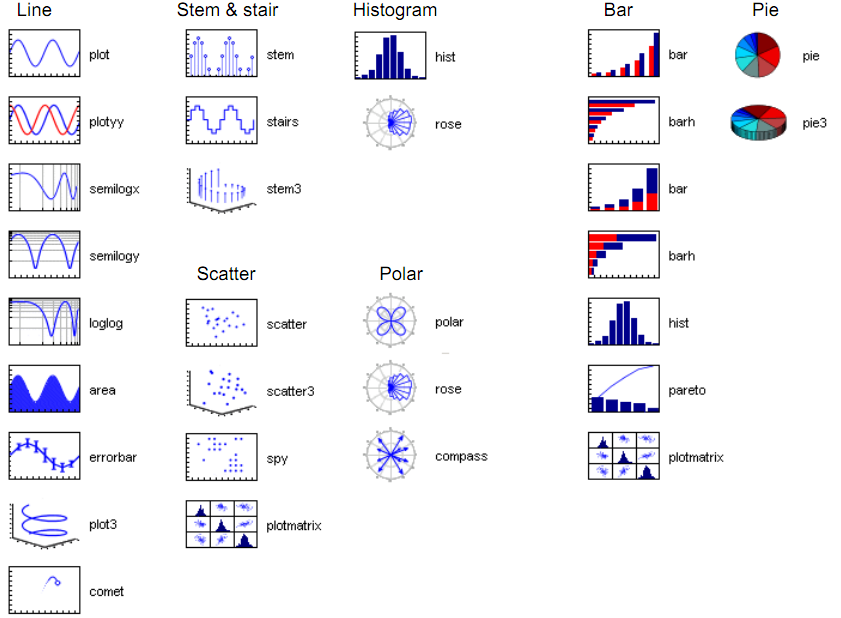
\includegraphics[width=450pt]{./Imagenes/graficos2d.png}
\end{center}

\section{Curvas en el plano}

Al construir la gráfica de una función $y=f(x)$ en el intervalo [a, b], se debe tener presente que \textbf{MATLAB} dibuja las curvas punto a punto; es decir, calcula los puntos $(x; f(x))$, para los valores de x que se le indique y representa dichos puntos unidos por un segmento. Por ello, se empieza estableciendo la matriz fila \textbf{x} cuyos elementos son los valores de \textbf{x} para los que se calculará el valor correspondiente de \textbf{f(x)}.

Para crear otros gráficos bi-dimensionales también se usa l comando \textbf{plot(x,y)}, donde los argumentos \textbf{x} e \textbf{y} son vectores con el mismo número de elementos.

Para representar una función del tipo $y=f(x)$ con el comando \textbf{plot}, el usuario necesita crear primero un vector con los valores de \textbf{x} del dominio de la función. En seguida, crear el vector $y=f(x)$ con los correspondientes valores de $f(x)$ y finalmente graficar la función $f$ con plot.

En el espacio de tres dimensiones la forma más sencilla de crear un gráfico 3D es mediante la 
función \textbf{plot3}, cuya sintaxis es bastante similar a la de la función \textbf{plot}. El comando \textbf{x=linspace(a,b,n)} crea el vector \textbf{x} de \textbf{n} elementos en el cual el primer elemento es \textbf{a} y el último es \textbf{b}, todos igualmente espaciados.

En \textbf{MATLAB} se usa el signo $\div$ para escribir los comentarios. Toda expresión después del signo $\div$ es ignorado por \textbf{MATLAB}. También usaremos los comandos \textbf{subplot}, \textbf{contour}, \textbf{contour3}, \textbf{quiver}, \textbf{comet}, etc.

Empezamos graficando funciones reales continuas definidas en un intervalo. Si $f$ es una función real de variable real, su gráfica es el conjunto $G(f)={(x;y)/y=f(x), x \in Dom(f)}$. Para comenzar vamos a estudiar en profundidad el comando \textbf{plot}, vamos ver algunos ejemplos con este comando y finalmente vamos a usar otros comandos que también sirven para representar curvas en el plano.

\section{El comando plot}

Los comandos de \textbf{MATLAB} cuentan con varios niveles de manipulación, y este es el caso del comando \textbf{plot}, el cual será fundamental para esta parte del curso. Los niveles iniciales son simples y por lo tanto fáciles de aprender y utilizar. El acceso a niveles finos exige trabajar con argumentos nuevos, más instrucciones y el manejo de una sintaxis más complicada. Comenzaremos viendo los diferentes niveles de forma gradual.

\subsection{Primer nivel}
El primer comando que trataremos es plot. Es una instrucción muy versátil y la más indicada para dibujar gráficas de funciones y curvas en el plano. Su sintaxis básica es

\begin{lstlisting}[language=Matlab]
>> plot(x,y)
\end{lstlisting}

que dibuja el vector y versus el vector x. Más en concreto une los puntos $(x_{i}, y_{i})$ mediante segmentos. Tomando un número suficientemente elevado de puntos trazamos con ello una gráfica suave, sin esquinas visibles.

Al ejecutar este comando se abre una ventana, \textbf{figure} en el vocabulario de \textbf{MATLAB}, donde se traza la correspondiente figura. Si \textbf{y} es real, \textbf{plot(y)} toma x=1:n donde n es la longitud de \textbf{y}. Si, por otro lado, y es un vector de números complejos, dibuja la parte imaginaria versus la parte real. Es decir, es equivalente a \textbf{plot(real(y),imag(y))}.

Las siguientes instrucciones utilizan el operador ":" (dos puntos) para crear un vector de los valores de \textbf{x} variando desde cero hasta 2 $\pi$ , para calcular el seno de estos valores y graficar el resultado.

\begin{lstlisting}[language=Matlab]
>> x = 0: pi/100 : 2*pi; 
>> y = sin(x); 
>> plot(x,y)
\end{lstlisting}

\begin{center}
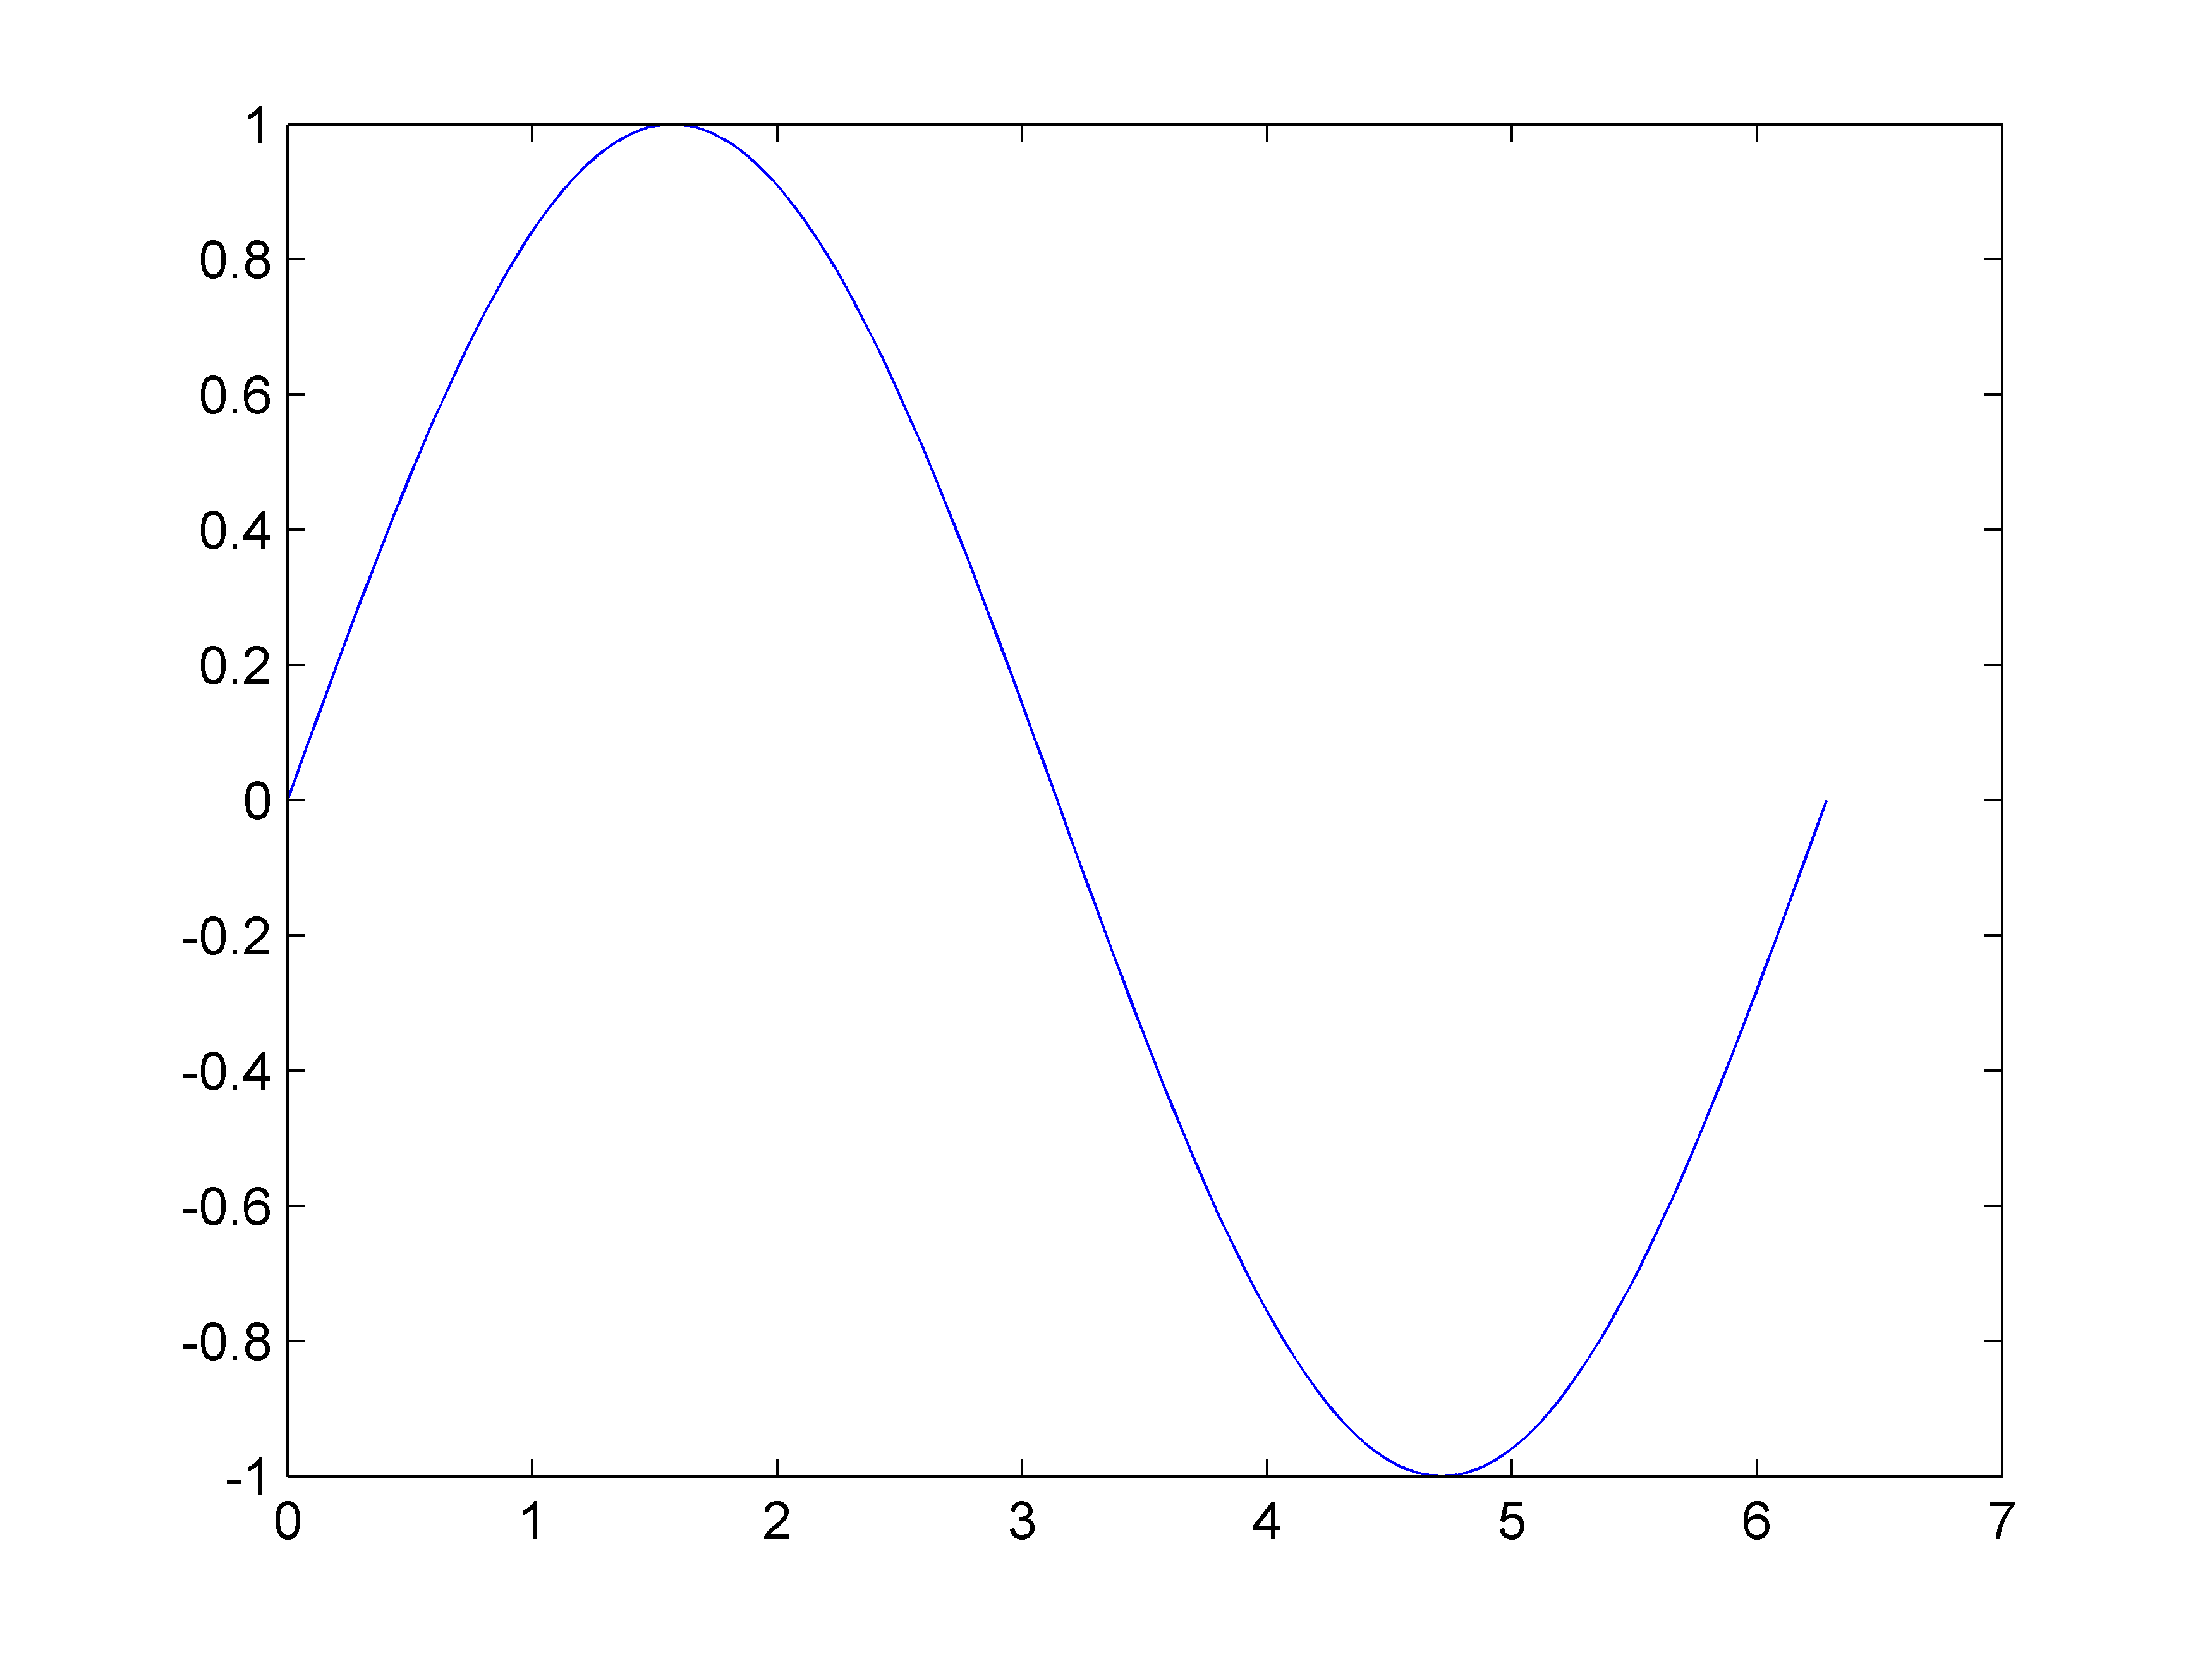
\includegraphics[width=300pt]{./Imagenes/seno1.png}
\end{center}

\subsubsection{Varias graficas en la misma imagen}

Múltiples pares de vectores x-y crean múltiples gráficos con una simple llamada a la sentencia 
plot. \textbf{MATLAB} les asigna automáticamente a través de una lista de colores predefinida (pero configurable por el usuario) para permitir la discriminación entre cada conjunto de datos. Por ejemplo, estas instrucciones grafican tres funciones de x, cada una con un color separado que las distingue. El comando \textbf{legend} provee una forma clara de identificar los gráficos individuales. 


\begin{lstlisting}[language=Matlab]
>> x = 0: pi/100 : 2*pi; 
>> y = sin(x);
>> y2 = sin(x-.25); 
>> y3 = sin(x-.5); 
>> plot(x,y,x,y2,x,y3)
>> legend('sin(x)','sin(x-.25)','sin(x-.5)'
\end{lstlisting}
\begin{center}
\includegraphics[width=300pt]{./Imagenes/senovarios.png}
\end{center}


\subsection{Segundo nivel}

El comando además acepta una serie de argumentos que, entre otras cosas, permiten controlar el color, el tipo de marcas sobre los puntos $(x_{i}, y_{i})$ y el formato de las líneas que los unen. Así, en su aspecto más general,

\begin{lstlisting}[language=Matlab]
>> plot(x,y,S)
\end{lstlisting}

dibuja y versus x, con S una cadena de caracteres que se construye con la primera columna especifica el color utilizado, la segunda la marca sobre cada punto y la tercera el patrón que siguen las líneas utilizadas para unir los puntos.

\begin{center}
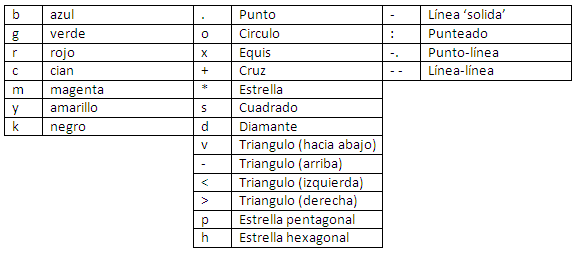
\includegraphics[width=300pt]{./Imagenes/comandosbasicos1.png}
\end{center}

La primer columna especifica el color utilizado, la segunda que tipo de marca se utilizara en cada punto y la tercer columna especifica el patrón que siguen las líneas utilizadas para unir los puntos.

\subsubsection{Líneas en gráficos}

En el caso de desearse una gráfica destinada a ser observada en blanco y negro, como por ejemplo  en fotocopias, conviene trazar líneas distintas en lugar de un tipo de línea y 
distintos colores. Por ejemplo, si la sentencia a usar es:

\begin{lstlisting}[language=Matlab]
>> x = 0: pi/100 : 2*pi; 
>> y = sin(x) 
>> y2 = sin(x-0.25) 
>> y3 = sin(x-0.5) 
>> plot (x,y,x,y2,':', x,y3,'--')
>> legend('sin(x)','sin(x-.25)','sin(x-.5)')
\end{lstlisting}
\begin{center}
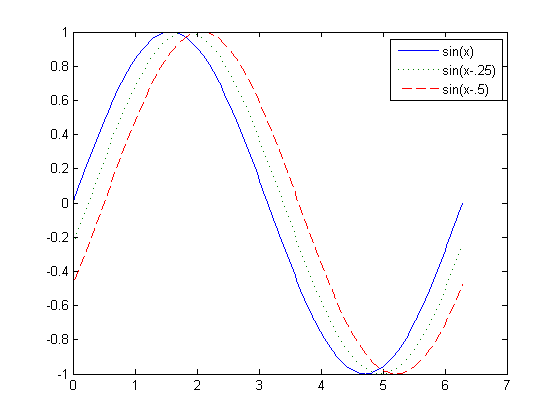
\includegraphics[width=300pt]{./Imagenes/senovariosmarca.png}
\end{center}

\subsubsection{Símbolos}

Si se especifica un tipo de símbolo pero no un estilo de línea, \textbf{MATLAB} exhibirá sólo el primero. Por ejemplo:

\begin{lstlisting}[language=Matlab]
>> clear 
>> x=0:0.02:2; 
>> y = 1 ./ ((x-.3).^2 + .01) + 1 ./ ((x-.9).^2 + .04) - 6; 
>> plot(x,y,'ks') 
\end{lstlisting}
\begin{center}
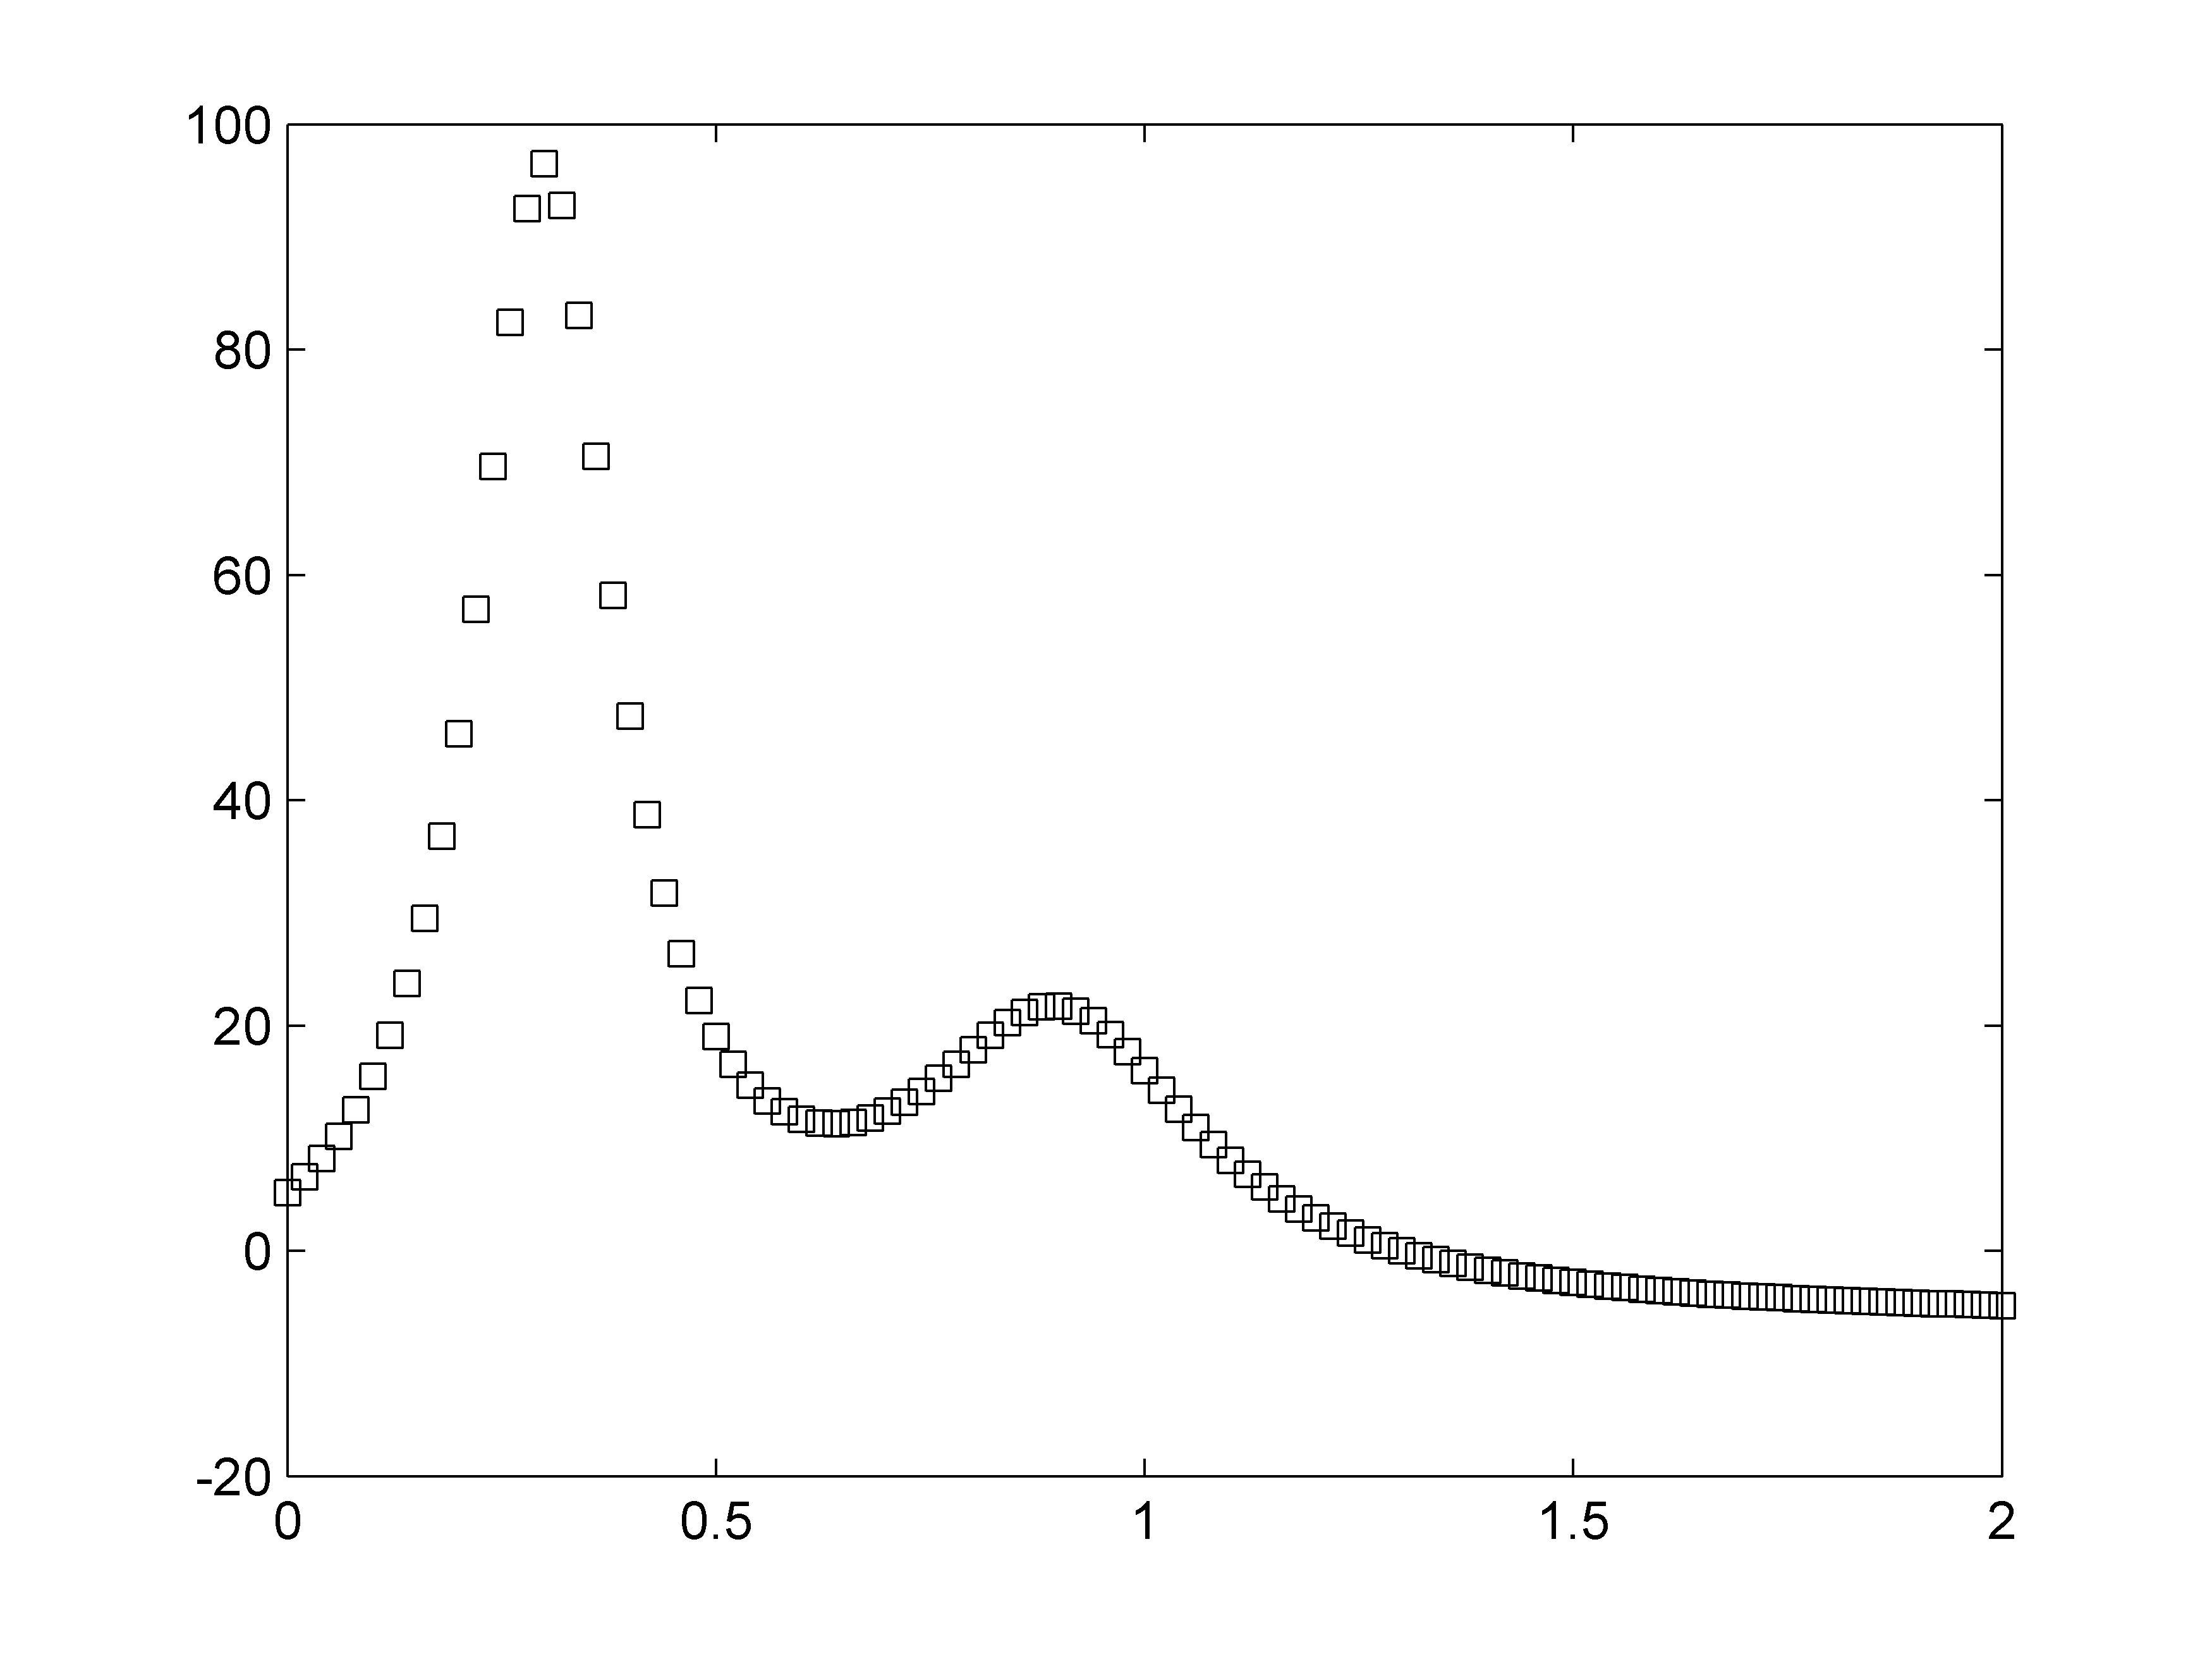
\includegraphics[width=300pt]{./Imagenes/simbolo1.png}
\end{center}

Si deseamos que aparezcan líneas con símbolos, se puede escribir, por ejemplo $plot(x,y,'r:+')$ 
que gráfica una línea roja de puntos y coloca marcadores de signo más en cada punto.:

\begin{lstlisting}[language=Matlab]
>> clear 
>> x=0:0.02:2; 
>> y = 1 ./ ((x-.3).^2 + .01) + 1 ./ ((x-.9).^2 + .04) - 6;
>> plot(x,y,'r:+')
\end{lstlisting}
\begin{center}
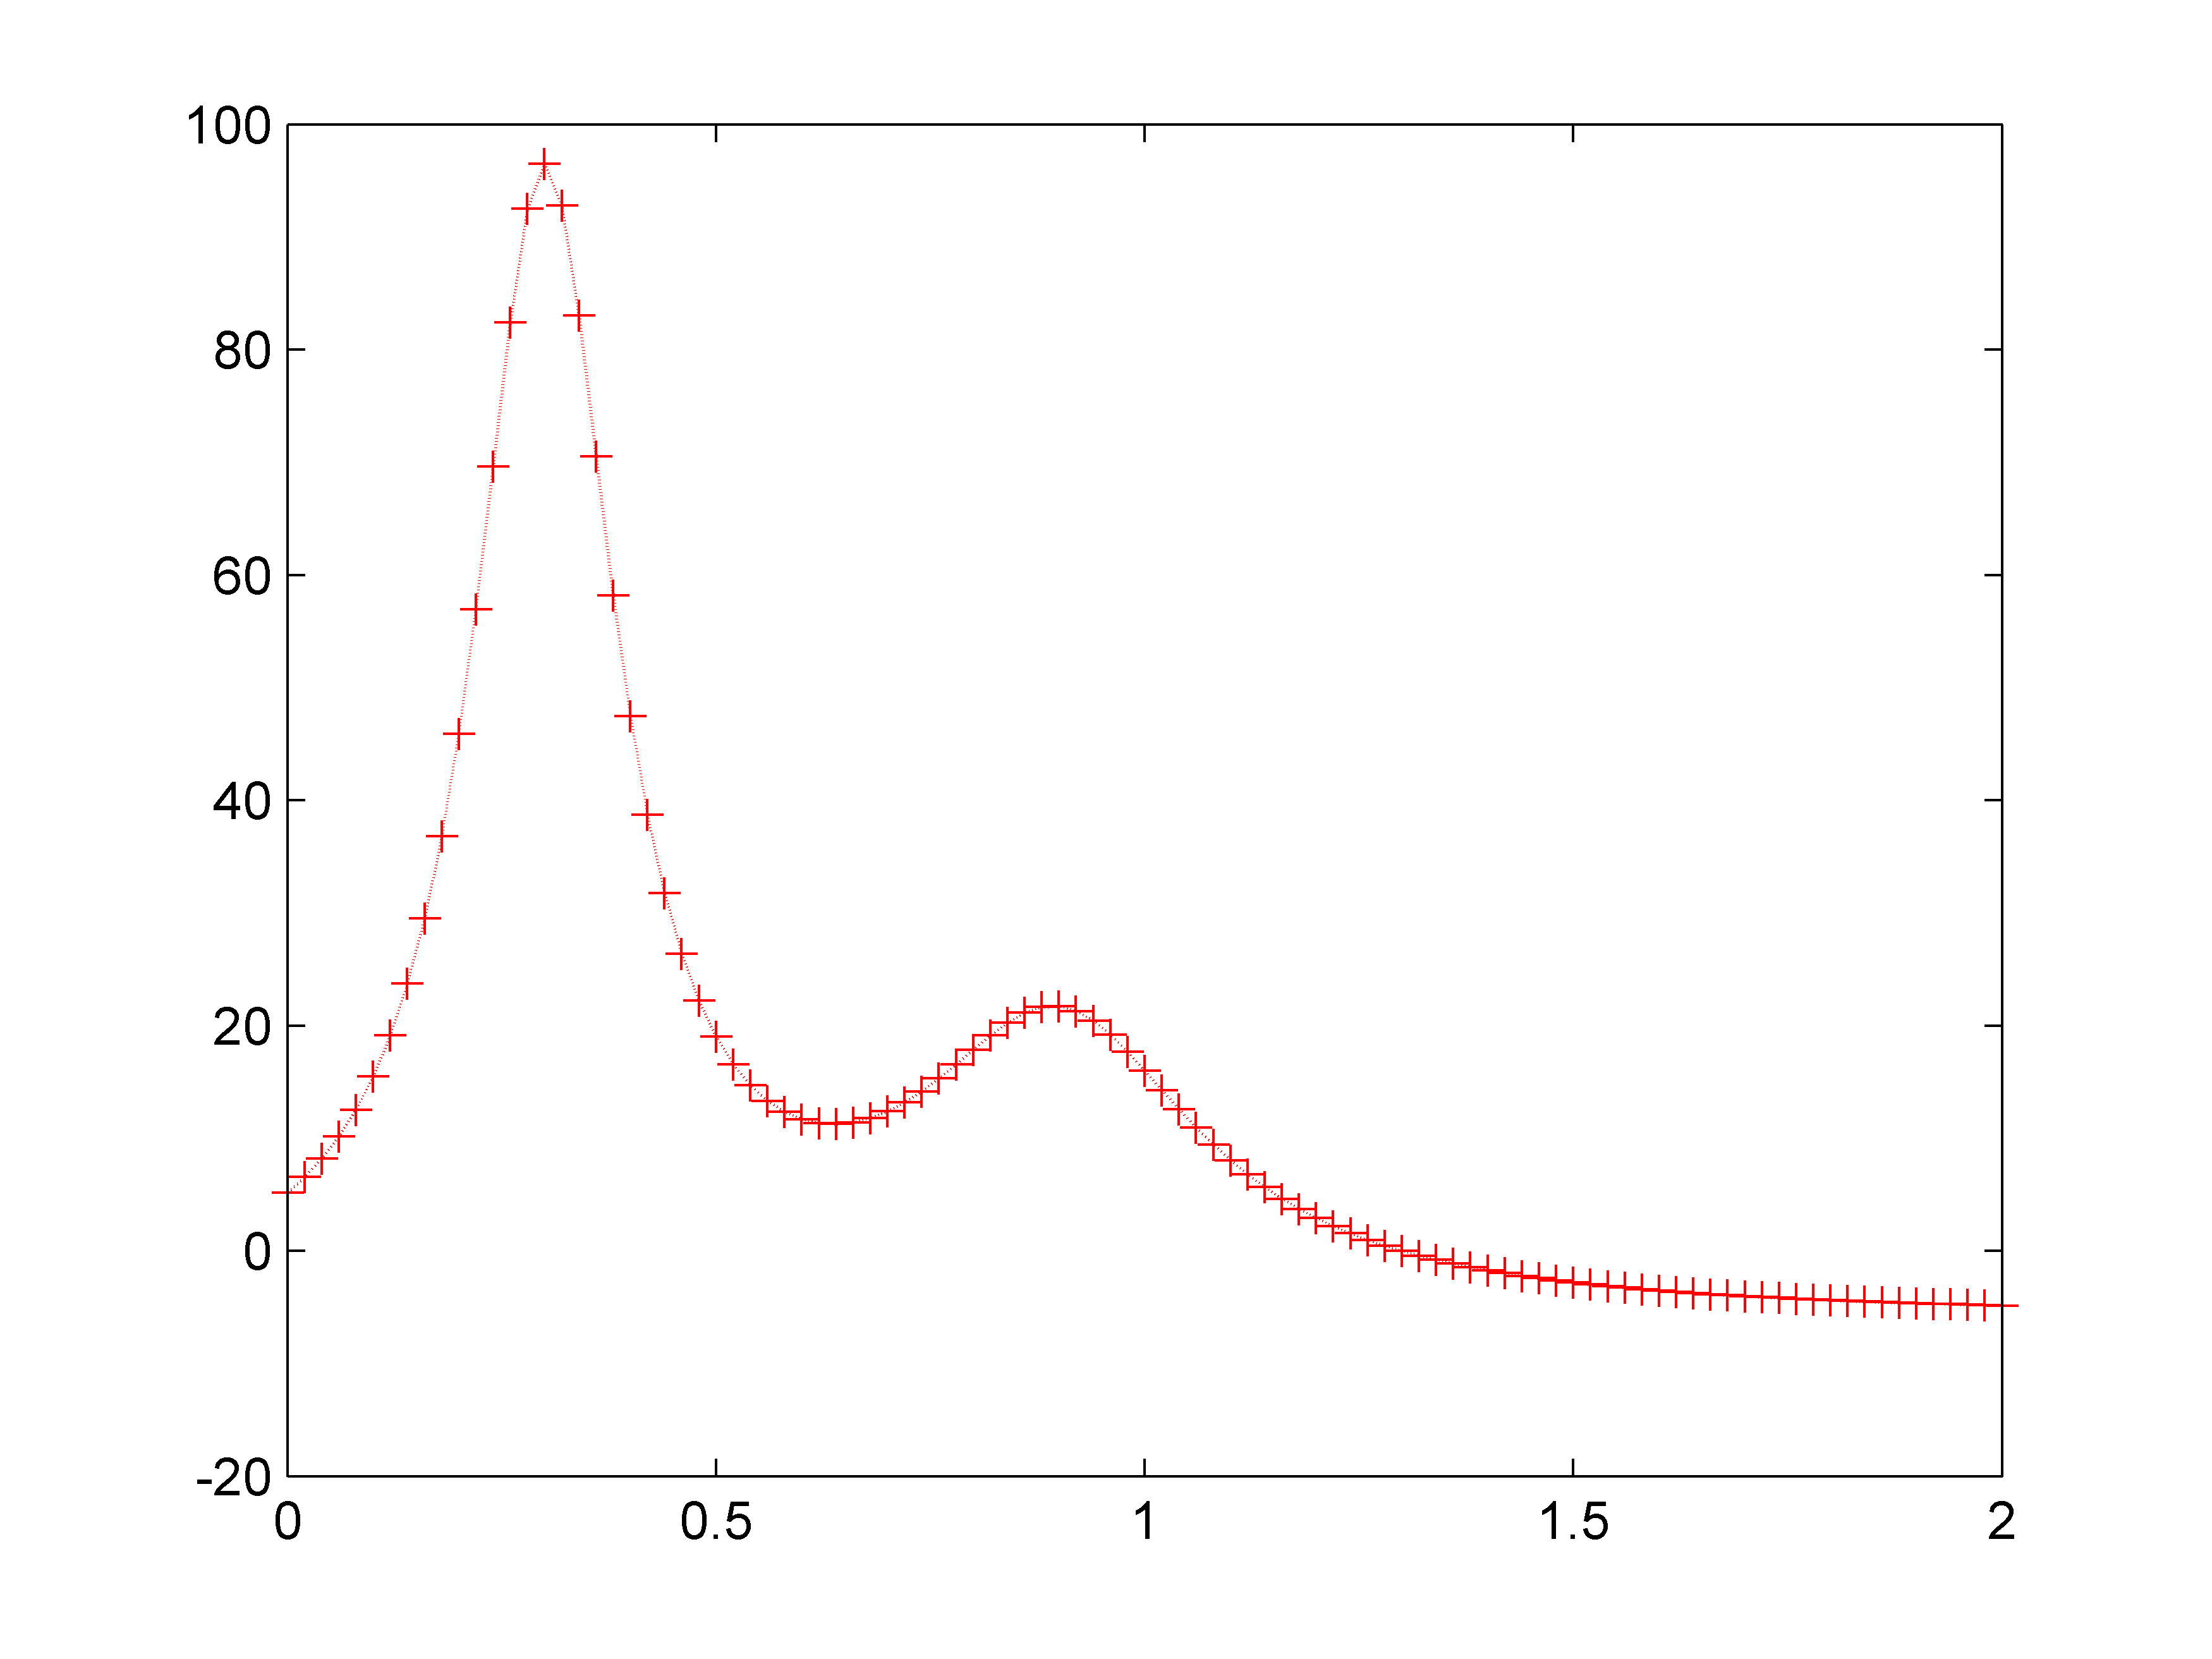
\includegraphics[width=300pt]{./Imagenes/simbolo2.png}
\end{center}

\subsubsection{Comandos hold on y hold off}

Normalmente, si se ejecuta una sentencia \textbf{plot}, y luego otra, en el curso de una sesión o 
programa, la ultima es la única que puede verse pues cada sentencia plot borra las anteriores. 
Por ejemplo:

\begin{lstlisting}[language=Matlab]
>> alfa = 0:0.02:2*pi; 
>> y = sin(alfa); 
>> plot (alfa,y) 
>> z = cos(alfa) 
>> plot(alfa,z)
\end{lstlisting}
 
permitiría visualizar sólo el gráfico del coseno, pero no el del seno. Una opción sería, como ya se vio, graficar conjuntamente las dos funciones, pero por distintas razones, surge a veces la necesidad de realizar una construcción secuencial de un gráfico para adicionar curvas 
gradualmente.  Esto se puede hacer mediante el uso de la sentencia \textbf{hold on} (sostener o mantener activo).

\begin{lstlisting}[language=Matlab]
>> x=0:0.02:2*pi; 
>> y = sin(x) 
>> plot(x,y) 
>> hold on 
>> z = cos(x) 
>> plot(x,z,':') 
>> hold off
\end{lstlisting}
\begin{center}
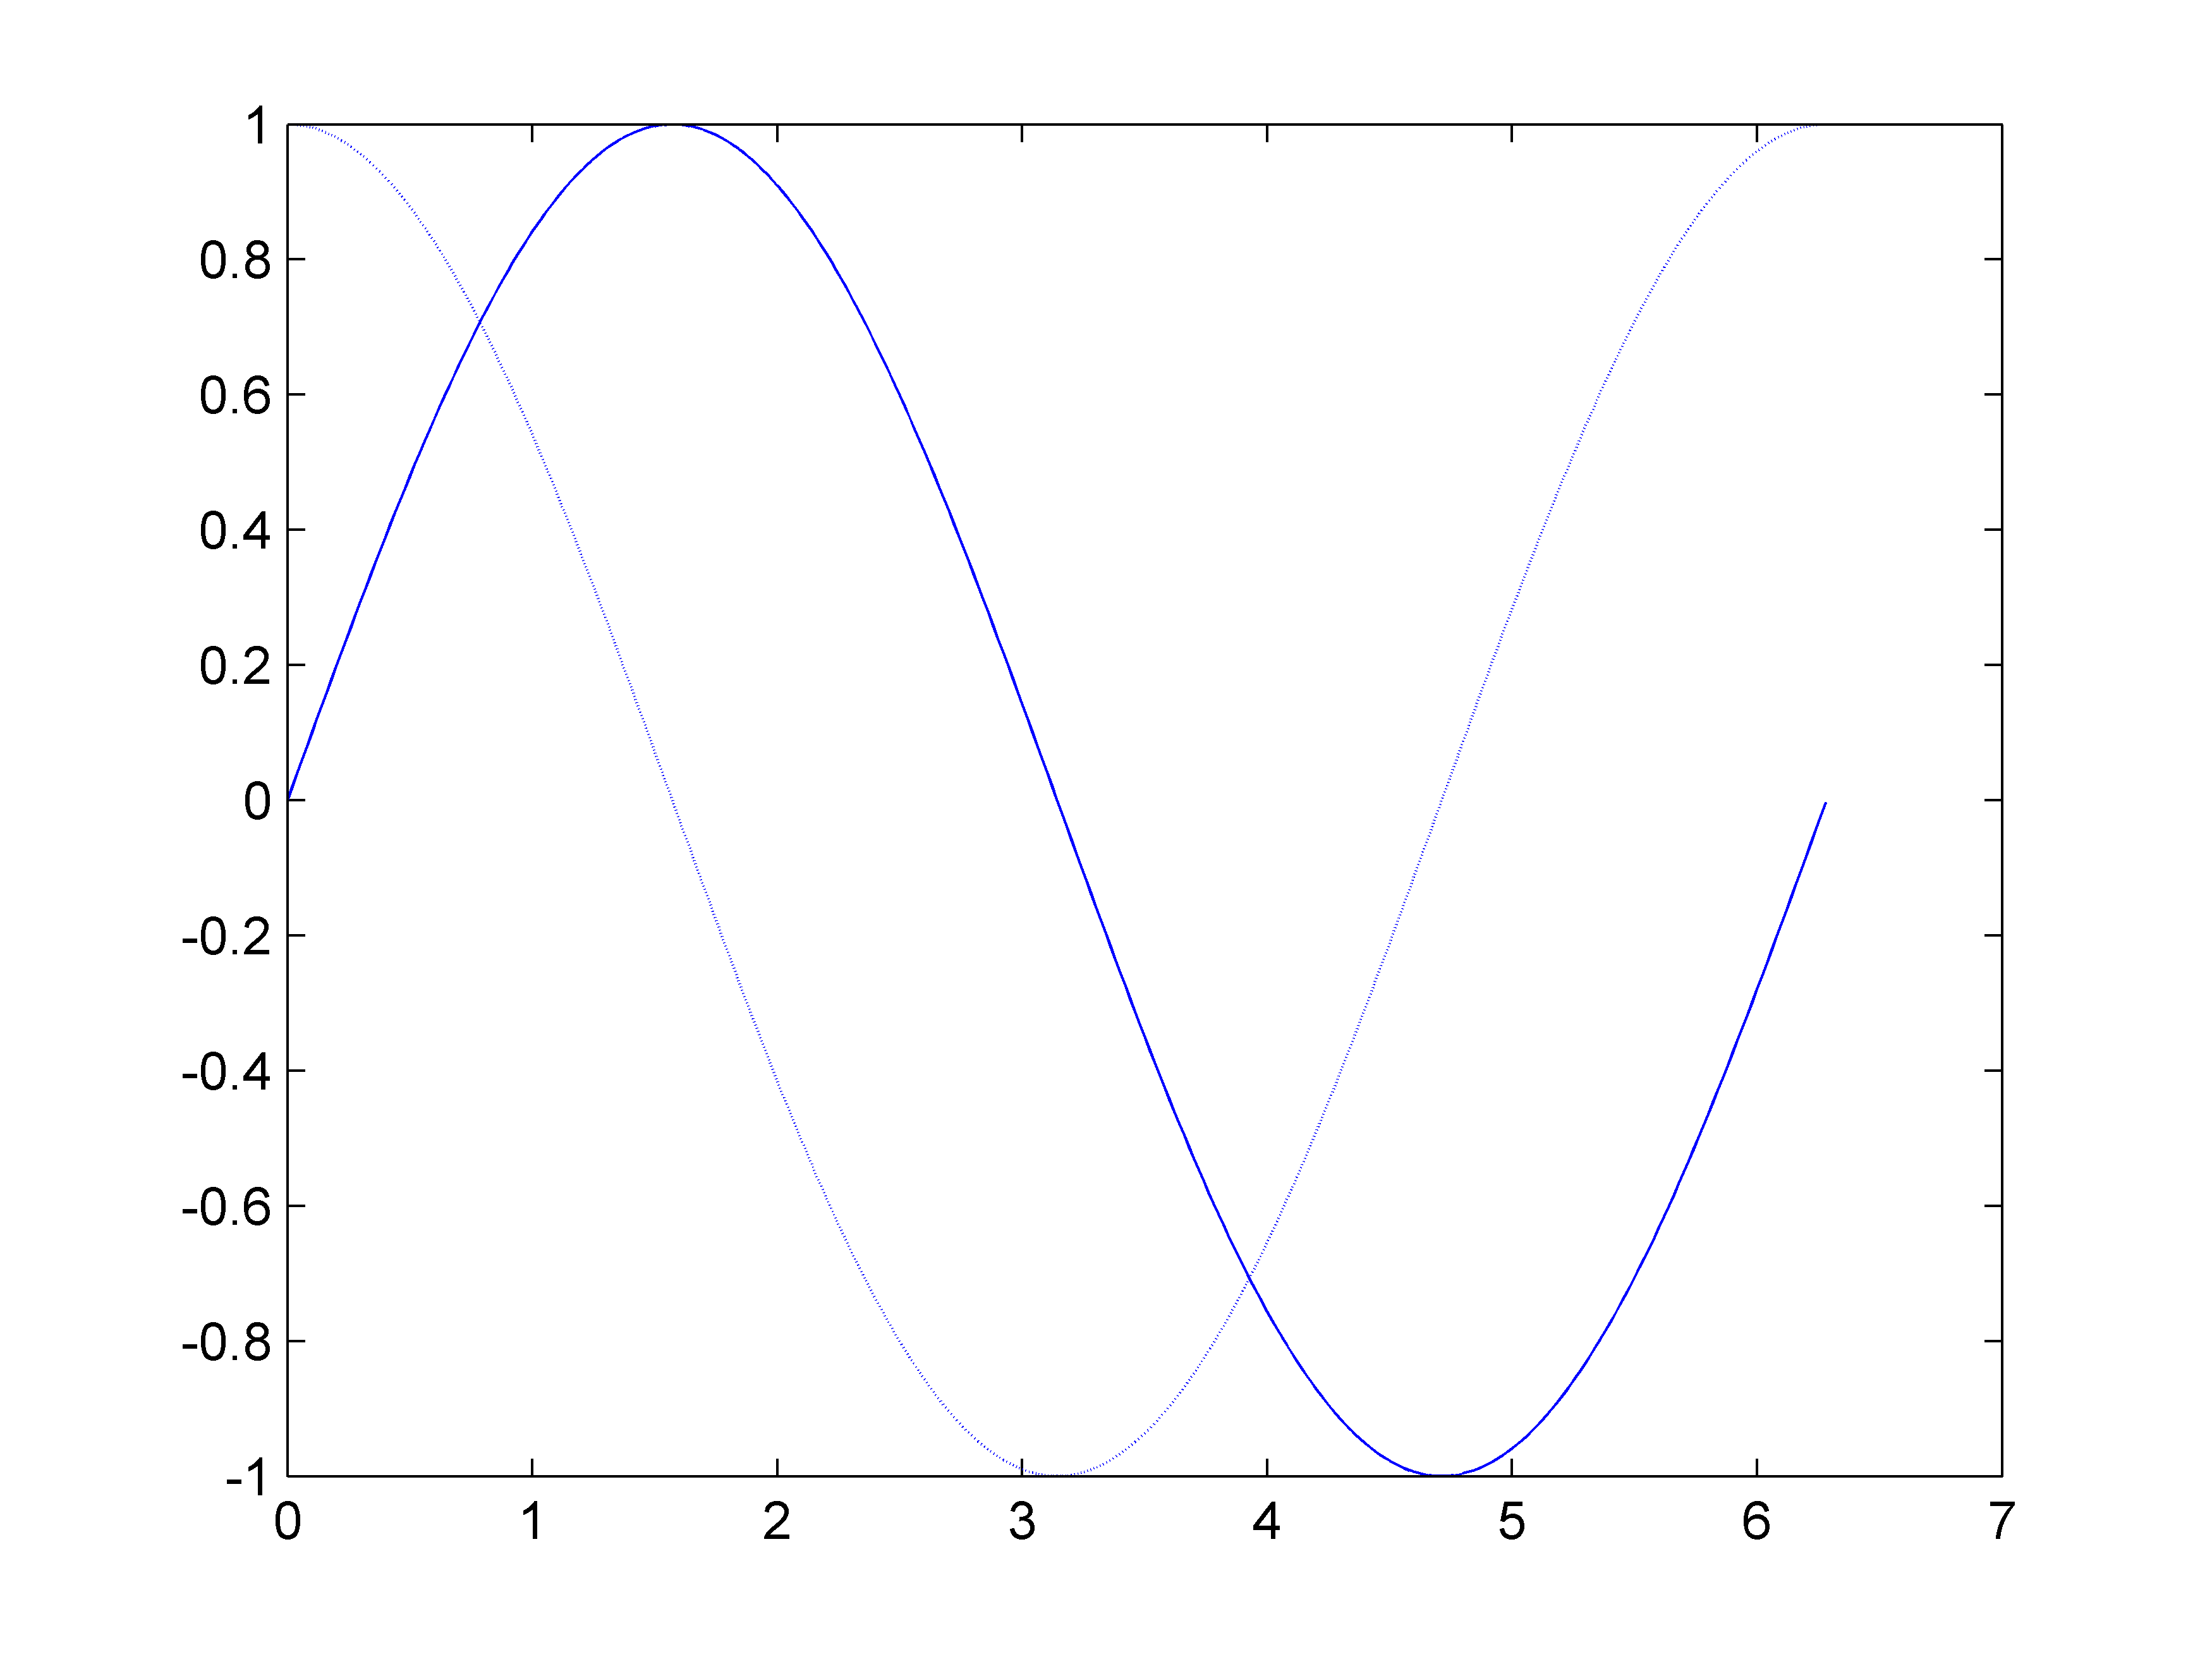
\includegraphics[width=300pt]{./Imagenes/holdon.png}
\end{center}

\subsubsection{Comando figure}

El comando \textbf{figure} permite mantener simultáneamente varias figuras para su observación, lo que resulta sumamente útil para evaluar los resultados de un programa. Por ejemplo:

\begin{lstlisting}[language=Matlab]
>> x = 0:0.02:2*pi; 
>> y = cos(x) 
>> z = exp(-x).*cos(x); 
>> plot(x,y) 
>> figure(2) 
>> plot(x,z) 
\end{lstlisting}

\subsubsection{Subdivisión de la ventana de gráficos}

A efectos de exhibir simultáneamente varias figuras sin solapamientos, se puede subdividir la 
ventana gráfica con la función subplot() en m particiones horizontales y n verticales. Cada una de esas particiones se puede llamar sub-gráfico. El subíndice \textit{i} identifica la subdivisión que se convierte en activa.

\begin{lstlisting}[language=Matlab]
>> x=0:0.1:10;
>> subplot(2,1,1), plot(x,sin(x));
>> subplot (2,1,2), plot(x,log(x))
\end{lstlisting}
\begin{center}
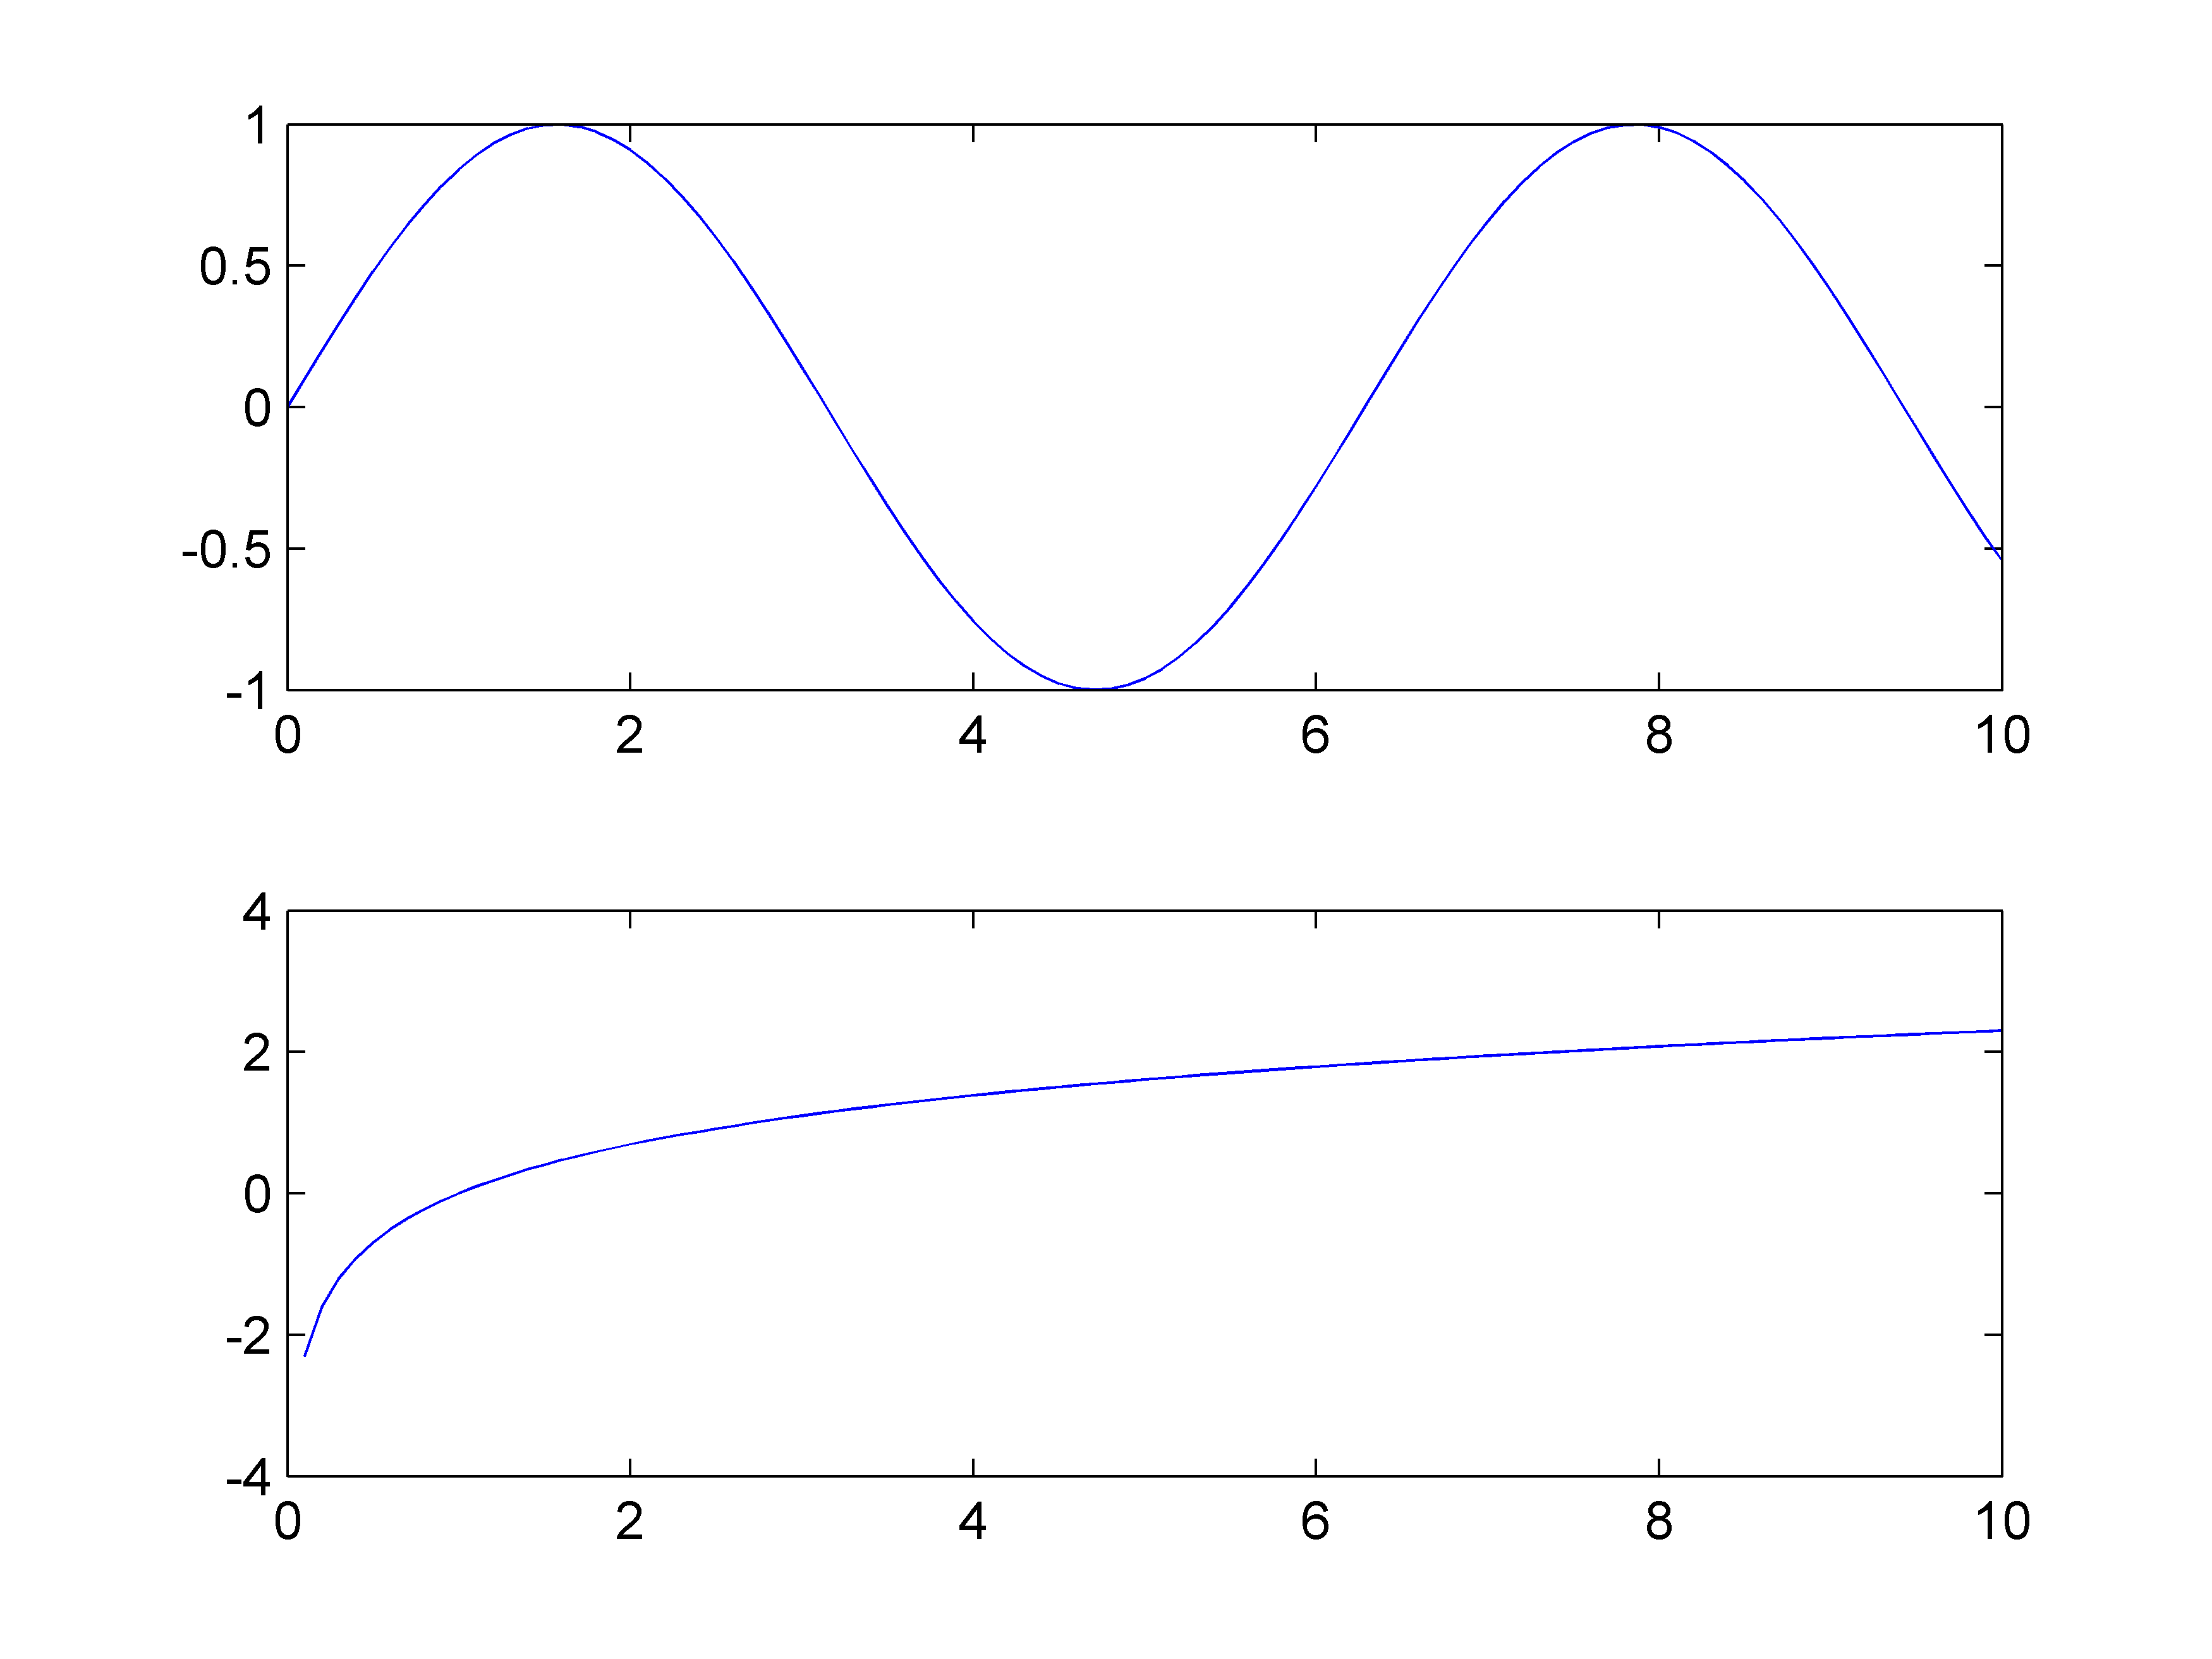
\includegraphics[width=300pt]{./Imagenes/subplot.png}
\end{center}

Ejemplo de subdivisión en dos filas y dos columnas:

\begin{lstlisting}[language=Matlab]
>> x=0: pi/25: 6*pi;  
>> y= cos(x); 
>> z= abs(cos(x))+1;  
>> w=exp(-0.2.*x).*y+ 2; 
>> v= exp(+0.2.*x).*y +2;  
>> subplot(2,2,1), plot(x,y); xlabel ('x', 'Fontsize', 18);ylabel('y','Fontsize', 18)  
>> subplot(2,2,2), plot(x,z); xlabel ('x', 'Fontsize', 18);ylabel('z', 'Fontsize', 18) 
>> subplot(2,2,3), plot(x,w);xlabel ('x', 'Fontsize', 18');ylabel('w','Fontsize', 18) 
>> subplot(2,2,4), plot(x,v); xlabel ('x', 'Fontsize', 18);ylabel('v', 'Fontsize', 18)
\end{lstlisting}
\begin{center}
\includegraphics[width=300pt]{./Imagenes/subplot2.png}
\end{center}


\subsection{Tercer nivel}

En este nivel se puede acceder a detalles concretos del gráfico como son el tamaño y el color de las marcas y el ancho de una linea entre otras cosas. Las diferentes opciones son:

\begin{itemize}
\item \textbf{color}: color de la linea.
\item \textbf{LineWidth}: ancho de una linea.
\item \textbf{Marker}: marca que se coloca en los puntos evaluados.
\item \textbf{MarkerEdgeColor}: color del borde de las marcas.
\item \textbf{MarkerFaceColor}: color de la marca.
\item \textbf{MarkerSize}: tamanio de la marca
\end{itemize}

Para especificar un color, se pueden utilizar los caracteres {b,g,r,c,m,y,k} o bien un vector con tres componentes con valores entre 0 y 1 que especifica un color según el estándar RGB. Un ejemplo del uso de estos comandos:

\begin{lstlisting}[language=Matlab]
>> x=0.01:0.2:2;
>> y=sin(x)./x;
>> plot(x,y,'o-.','color',[0.2 0.4 0.6],'linewidth',2,'markeredgecolor',...
'k','markerfacecolor',[0.9 0.6 0.4],'markersize',9)
\end{lstlisting}
\begin{center}
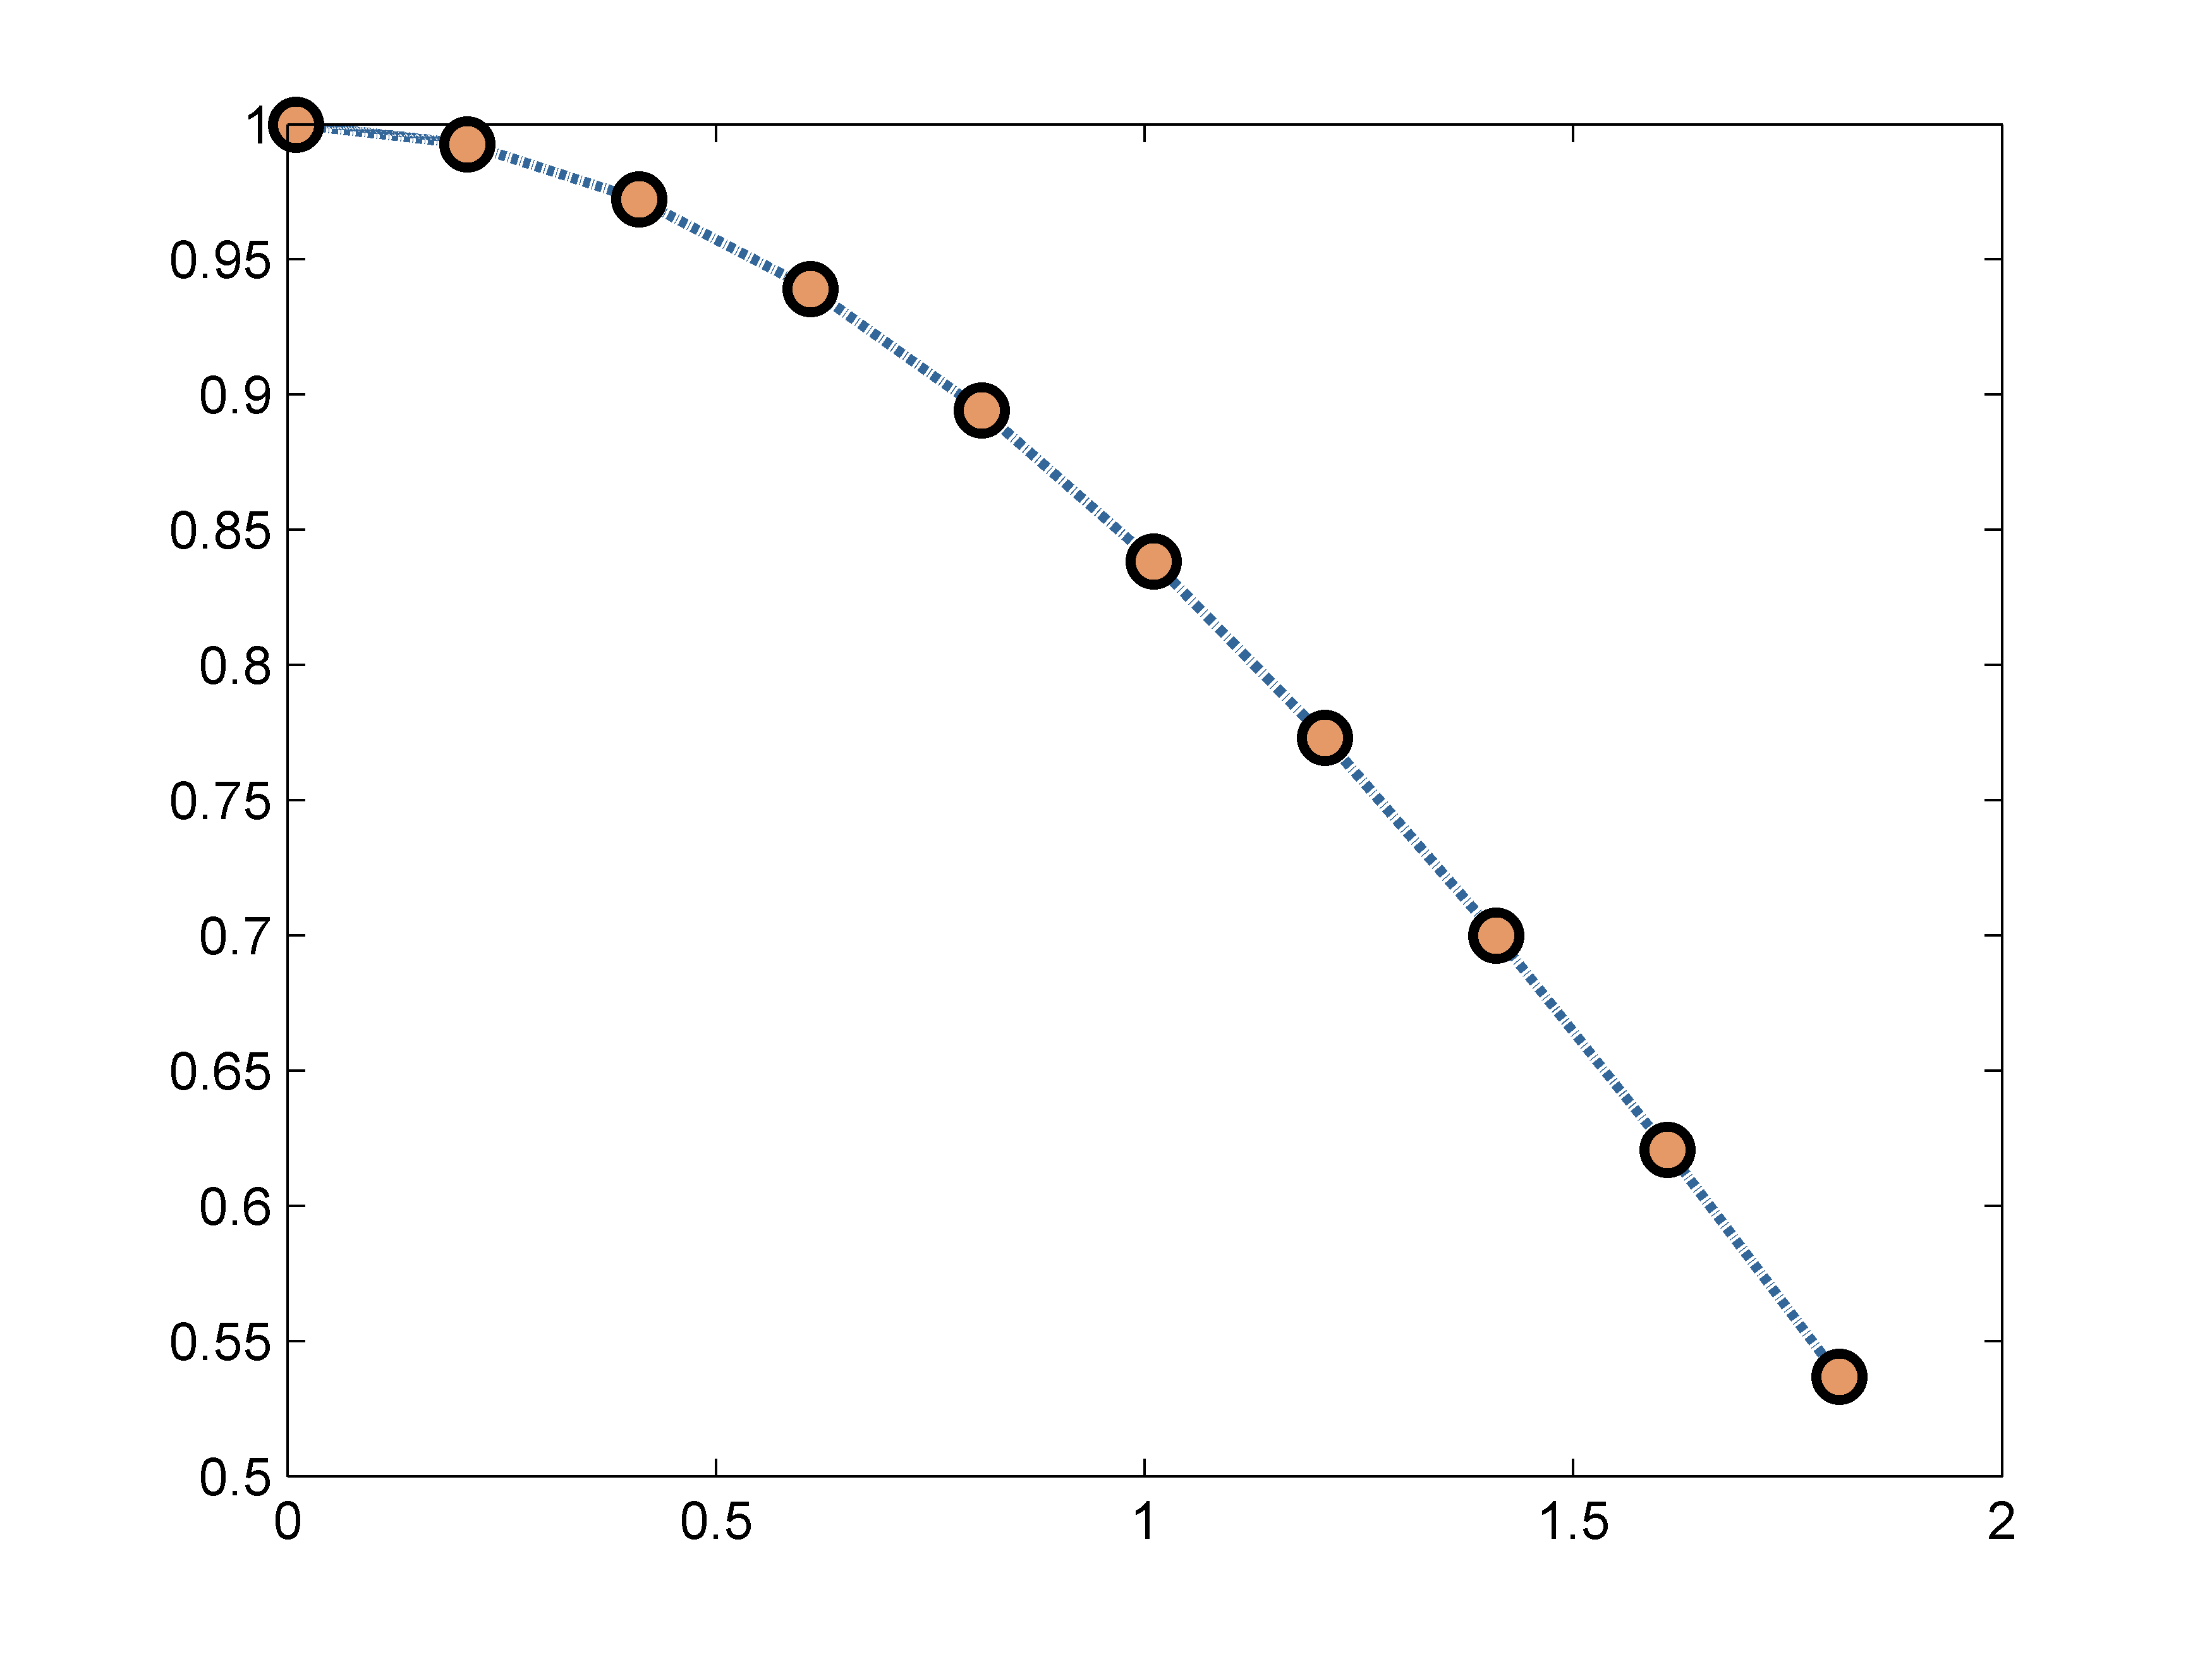
\includegraphics[width=300pt]{./Imagenes/tercernivel.png}
\end{center}

\section{Comandos asociados a plot}

Hay comandos que nos permiten controlar la ventana donde se mostraran los gráficos. Entre los más usados están:

\begin{itemize}
\item \textbf{clf}: borra la ventana actual (figure) de gráficos.
\item \textbf{cla}: borra los ejes.
\item \textbf{hold}: nos permite solapar varias gráficas en una misma ventana.
\item \textbf{axis}: puede controlar los ejes X e Y.
\item \textbf{xlim,ylim}: especifica los limites del dibujo. Se pueden utilizar para centrarlo.
\item \textbf{grid}: grid on muestra una malla en pantalla, y grid off la borra.
\item \textbf{legend}: despliega una leyenda, esto es, un cuadro detallando las gráficas.
\item \textbf{text}: ingresar un texto
\item \textbf{xlabel,ylabel}: etiqueta los ejes X e Y.
\item \textbf{title}: coloca un titulo en la cabecera del dibujo.
\item \textbf{whitebg}: asigna un color al fondo de la figura.
\end{itemize}

A continuación vamos a ver un ejemplo donde representamos 4 funciones, y usamos varios de los comandos antes mencionados para tratar los datos de la ventana y de los gráficos en si:

\begin{lstlisting}[language=Matlab]
>> figure(1) % desplegamos ventana 1
>> clf % borramos todo
>> x=linspace(0,5,100);
>> f=inline('exp(-n*x).*cos(x)','n','x'); % funciones vectorizadas
>> hold on % solapamiento de graficas
>> y=f(1/3,x);
>> plot(x,y,'k--','linewidth',2)
>> y=f(1,x);
>> plot(x,y,'r-.','linewidth',2)
>> y=f(3,x);
>> plot(x,y,':','color',[0.0,0.0,0.5],'linewidth',2)
>> y=f(9,x);
>> plot(x,y,'-','color',[0.0,0.3,0.0],'linewidth',2)
>> grid on % desplegamos la red
>> xlim([-0.5,6]), ylim([-0.25,0.5]) % rango de los graficos
>> xlabel('Eje X','fontname', 'Comic Sans Ms', 'fontsize',12)
>> ylabel('Eje Y','fontname', 'Comic Sans Ms', 'fontsize',12)
>> title('Graficas de ejemplo','fontsize',16,'fontname','Times new roman')
>> legend('exp(-x/3).*cos(x)', 'exp(-x).*cos(x)','exp(-3x)*cos(x)', 'exp(-9x).*cos(x)');
\end{lstlisting}
\begin{center}
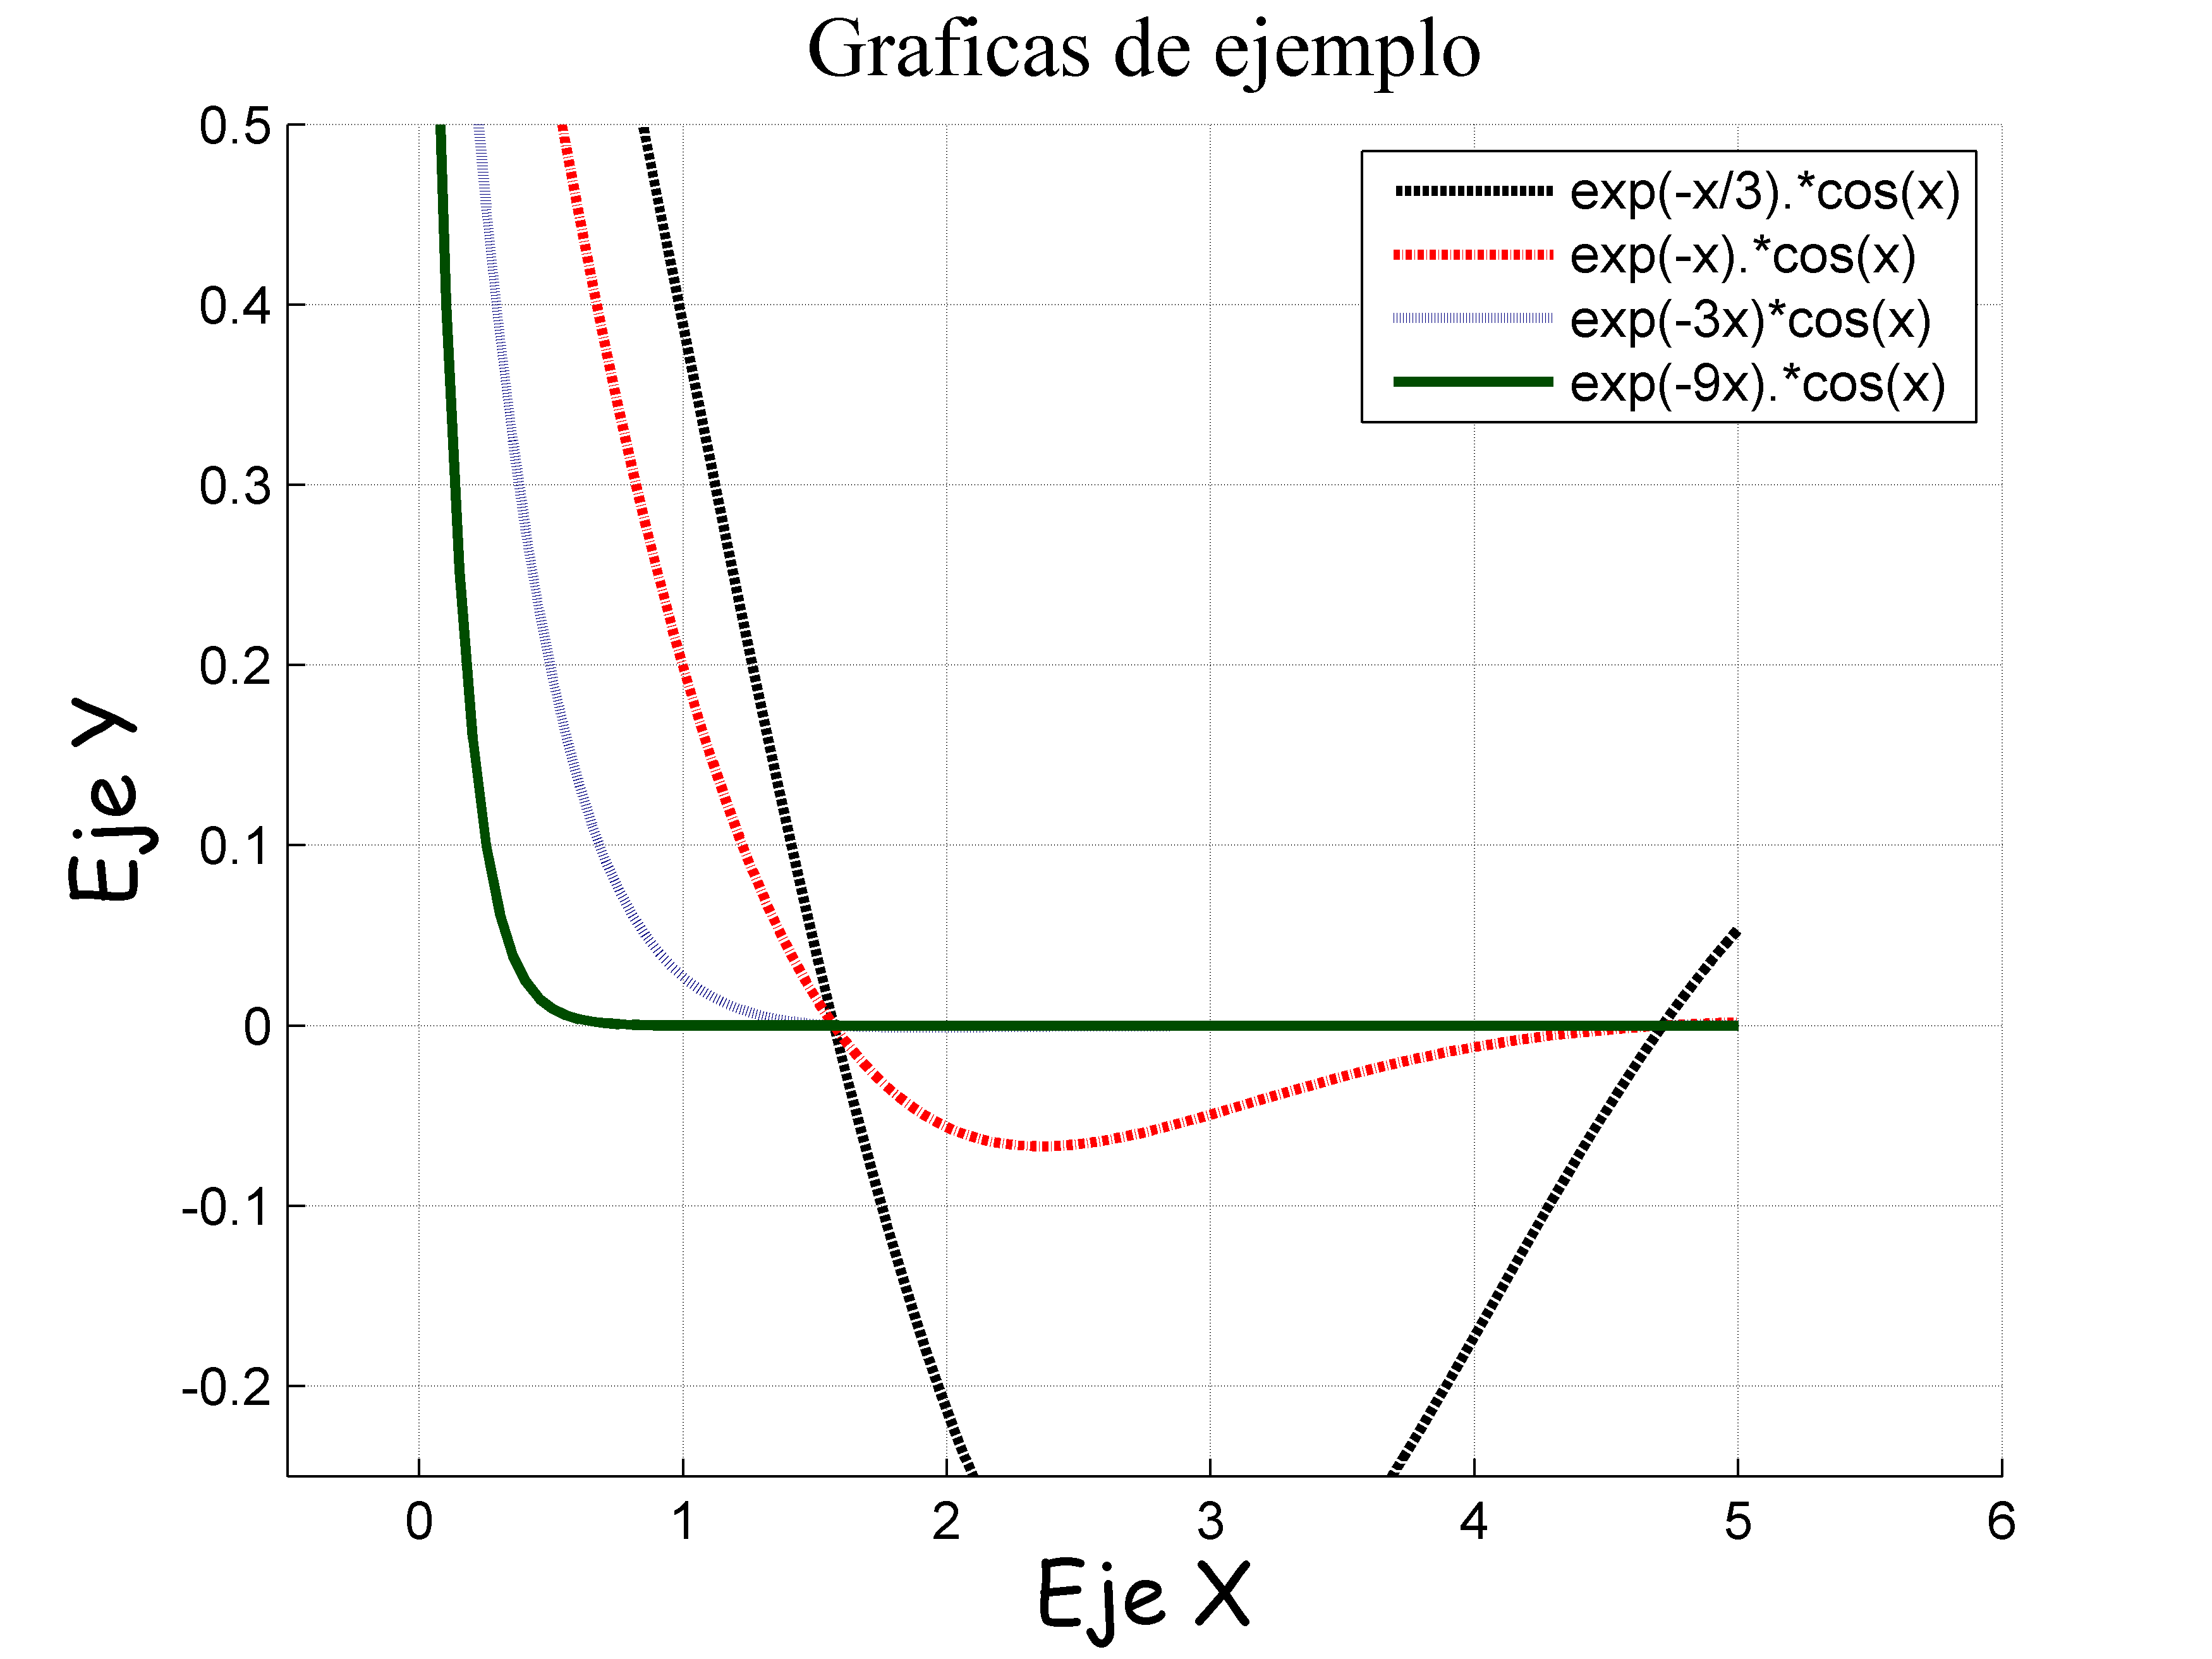
\includegraphics[width=300pt]{./Imagenes/plotas.png}
\end{center}





\section{Otros tipos de salidas gráficas}

Además del comando \textbf{plot}, hay otros comandos que permiten realizar gráficos bi-dimensionales, y que tienen un manejo similar al de este comando. Estos comandos son:

\begin{itemize}
\item \textbf{plotyy}: permite mostrar dos gráficos en la misma ventana con dos ejes Y a la izquierda y a la derecha.
\item \textbf{polar}: curvas en polares
\item \textbf{semilogx, semilogy}: similar a plot, pero usando una escala logarítmica en los ejes X e Y.
\item \textbf{loglog}: escala logarítmica en ambos ejes.
\item \textbf{stem}: dibuja uniéndolos con una linea vertical al eje X.
\item \textbf{stairs}: traza una gráfica en forma de escalera.
\item \textbf{bar, barh, bar3}: despliega gráficas en forma de barras. Útil para representar datos estadísticos.
\item \textbf{area}: muestra los datos en una gráfica d forma acumulada. El color se controla con el comando colormap. 
\item \textbf{line}: un puntos mediante líneas. Instrucción de bajo nivel que da origen a plot.
\item \textbf{fill}: dibuja polígonos cerrados y colora su interior.
\item \textbf{patch}: construye polígonos o caras en 3 dimensiones y asigna un color a la cara definida.
\end{itemize}

\section{Gráficos de funciones}

\textbf{MATLAB} tiene una serie de comandos asociados al Toolbox de calculo simbólico, los cuales nos permiten obtener la gráfica  d las funciones más conocidas. En esa sección podremos observar como quedan representadas las funciones más comunes.

\subsubsection{Función lineal}

\begin{enumerate}

\item \textbf{Ejemplo 1}: función $y = x + 2$
\begin{lstlisting}[language=Matlab]
>> x = [1:1:10]

x =

     1     2     3     4     5     6     7     8     9    10

>> y = x+2;
>> plot(y)
\end{lstlisting}
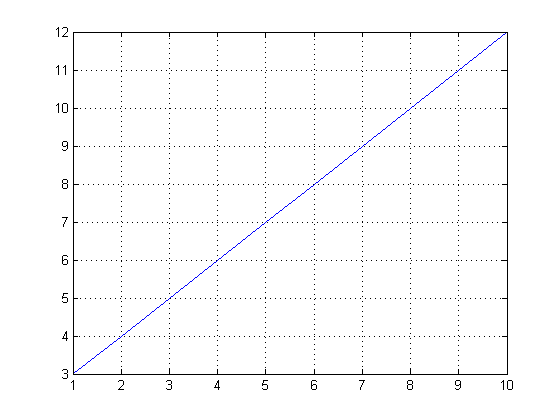
\includegraphics[width=300pt]{./Imagenes/ejem1.png}

\item \textbf{Ejemplo 2}: función $y = -x + 2$
\begin{lstlisting}[language=Matlab]
>> y = -x+2;
>> plot(y)
>> grid
\end{lstlisting}
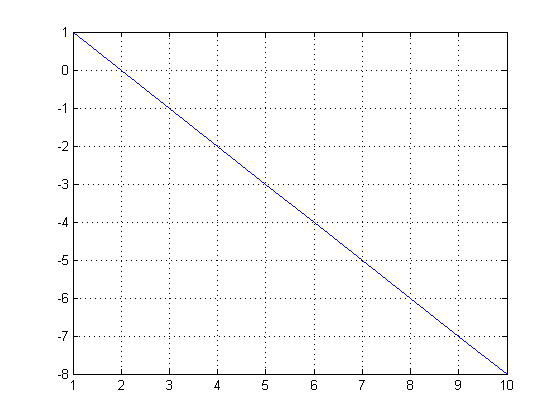
\includegraphics[width=300pt]{./Imagenes/ejem2.png}
\end{enumerate}

\subsubsection{Función raíz cuadrada}

\begin{enumerate}
\item \textbf{Ejemplo 1}: función $y = \sqrt{t}$
\begin{lstlisting}[language=Matlab]
>> t = 0:.05:4*pi;
>> y = sqrt(t);
>> plot(t,y)
>> grid
\end{lstlisting}
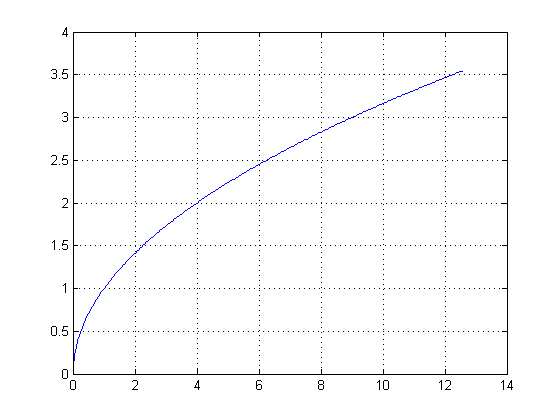
\includegraphics[width=300pt]{./Imagenes/ejem13.png}
\end{enumerate}


\subsubsection{Función exponencial}

\begin{enumerate}

\item \textbf{Ejemplo 1}: función $y = 2^{t}$
\begin{lstlisting}[language=Matlab]
>> t = 0:.05:4*pi;
>> y = 2.^(t);
>> plot(t,y)
>> grid
\end{lstlisting}
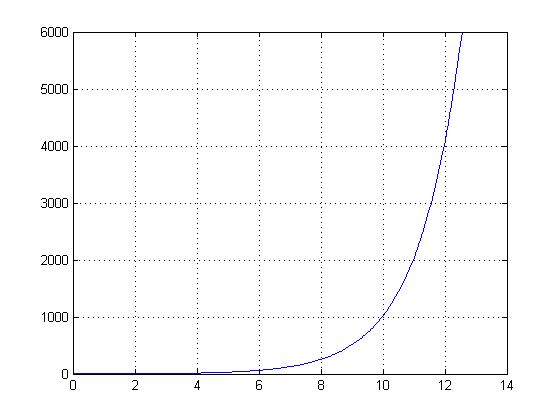
\includegraphics[width=300pt]{./Imagenes/ejem14.png}
\end{enumerate}



\section{Graficar observaciones y predicciones}

Es muy frecuente en ingeniería comparar las observaciones medidas (por ejemplo la temperatura 
ambiente) con los cálculos realizados mediante un modelo matemático (sea éste meramente una 
función algebraica ajustada previamente a los datos, o un modelo teórico que interprete la física del sistema). El siguiente programa ilustra un ejercicio, donde se comparan datos de un día lluvioso, con un polinomio de grado 5 ajustado a ellos. Incidentalmente se muestran las útiles funciones pre-programadas de \textbf{MATLAB}, \textbf{polyfit} que devuelve el vector de coeficientes del polinomio ajustado según el método de los cuadrados mínimos y \textbf{polyval} que calcula los valores del polinomio dado el vector de coeficientes y el vector de la variable 
independiente, t.

\begin{lstlisting}[language=Matlab]
>> clear 
>> t = 0:1:23; 
>> T = [12 11.5 10.9 9.8 9.4 8.7 8.5 8.9 10.1 11.3 12.1 13 14 14.5 14.8 15.1 15.4 15.2... 
        15.1 14.7 14.2 13.9 13.6 12.8 ]; 
>> p = polyfit (t, T,5) 
>  Tp = polyval(p,t) 
>> plot (t,T, 'o', t, Tp, 'Linewidth', 1); 
>> Title ('DIA LLUVIOSO', 'Fontsize', 25) 
>> xlabel ('Hora', 'Fontsize', 20) 
>> ylabel ('Temperatura', 'Fontsize', 20) 
>> legend ('Datos del SMN', 'Polynomio grado 5') 
\end{lstlisting}
\begin{center}
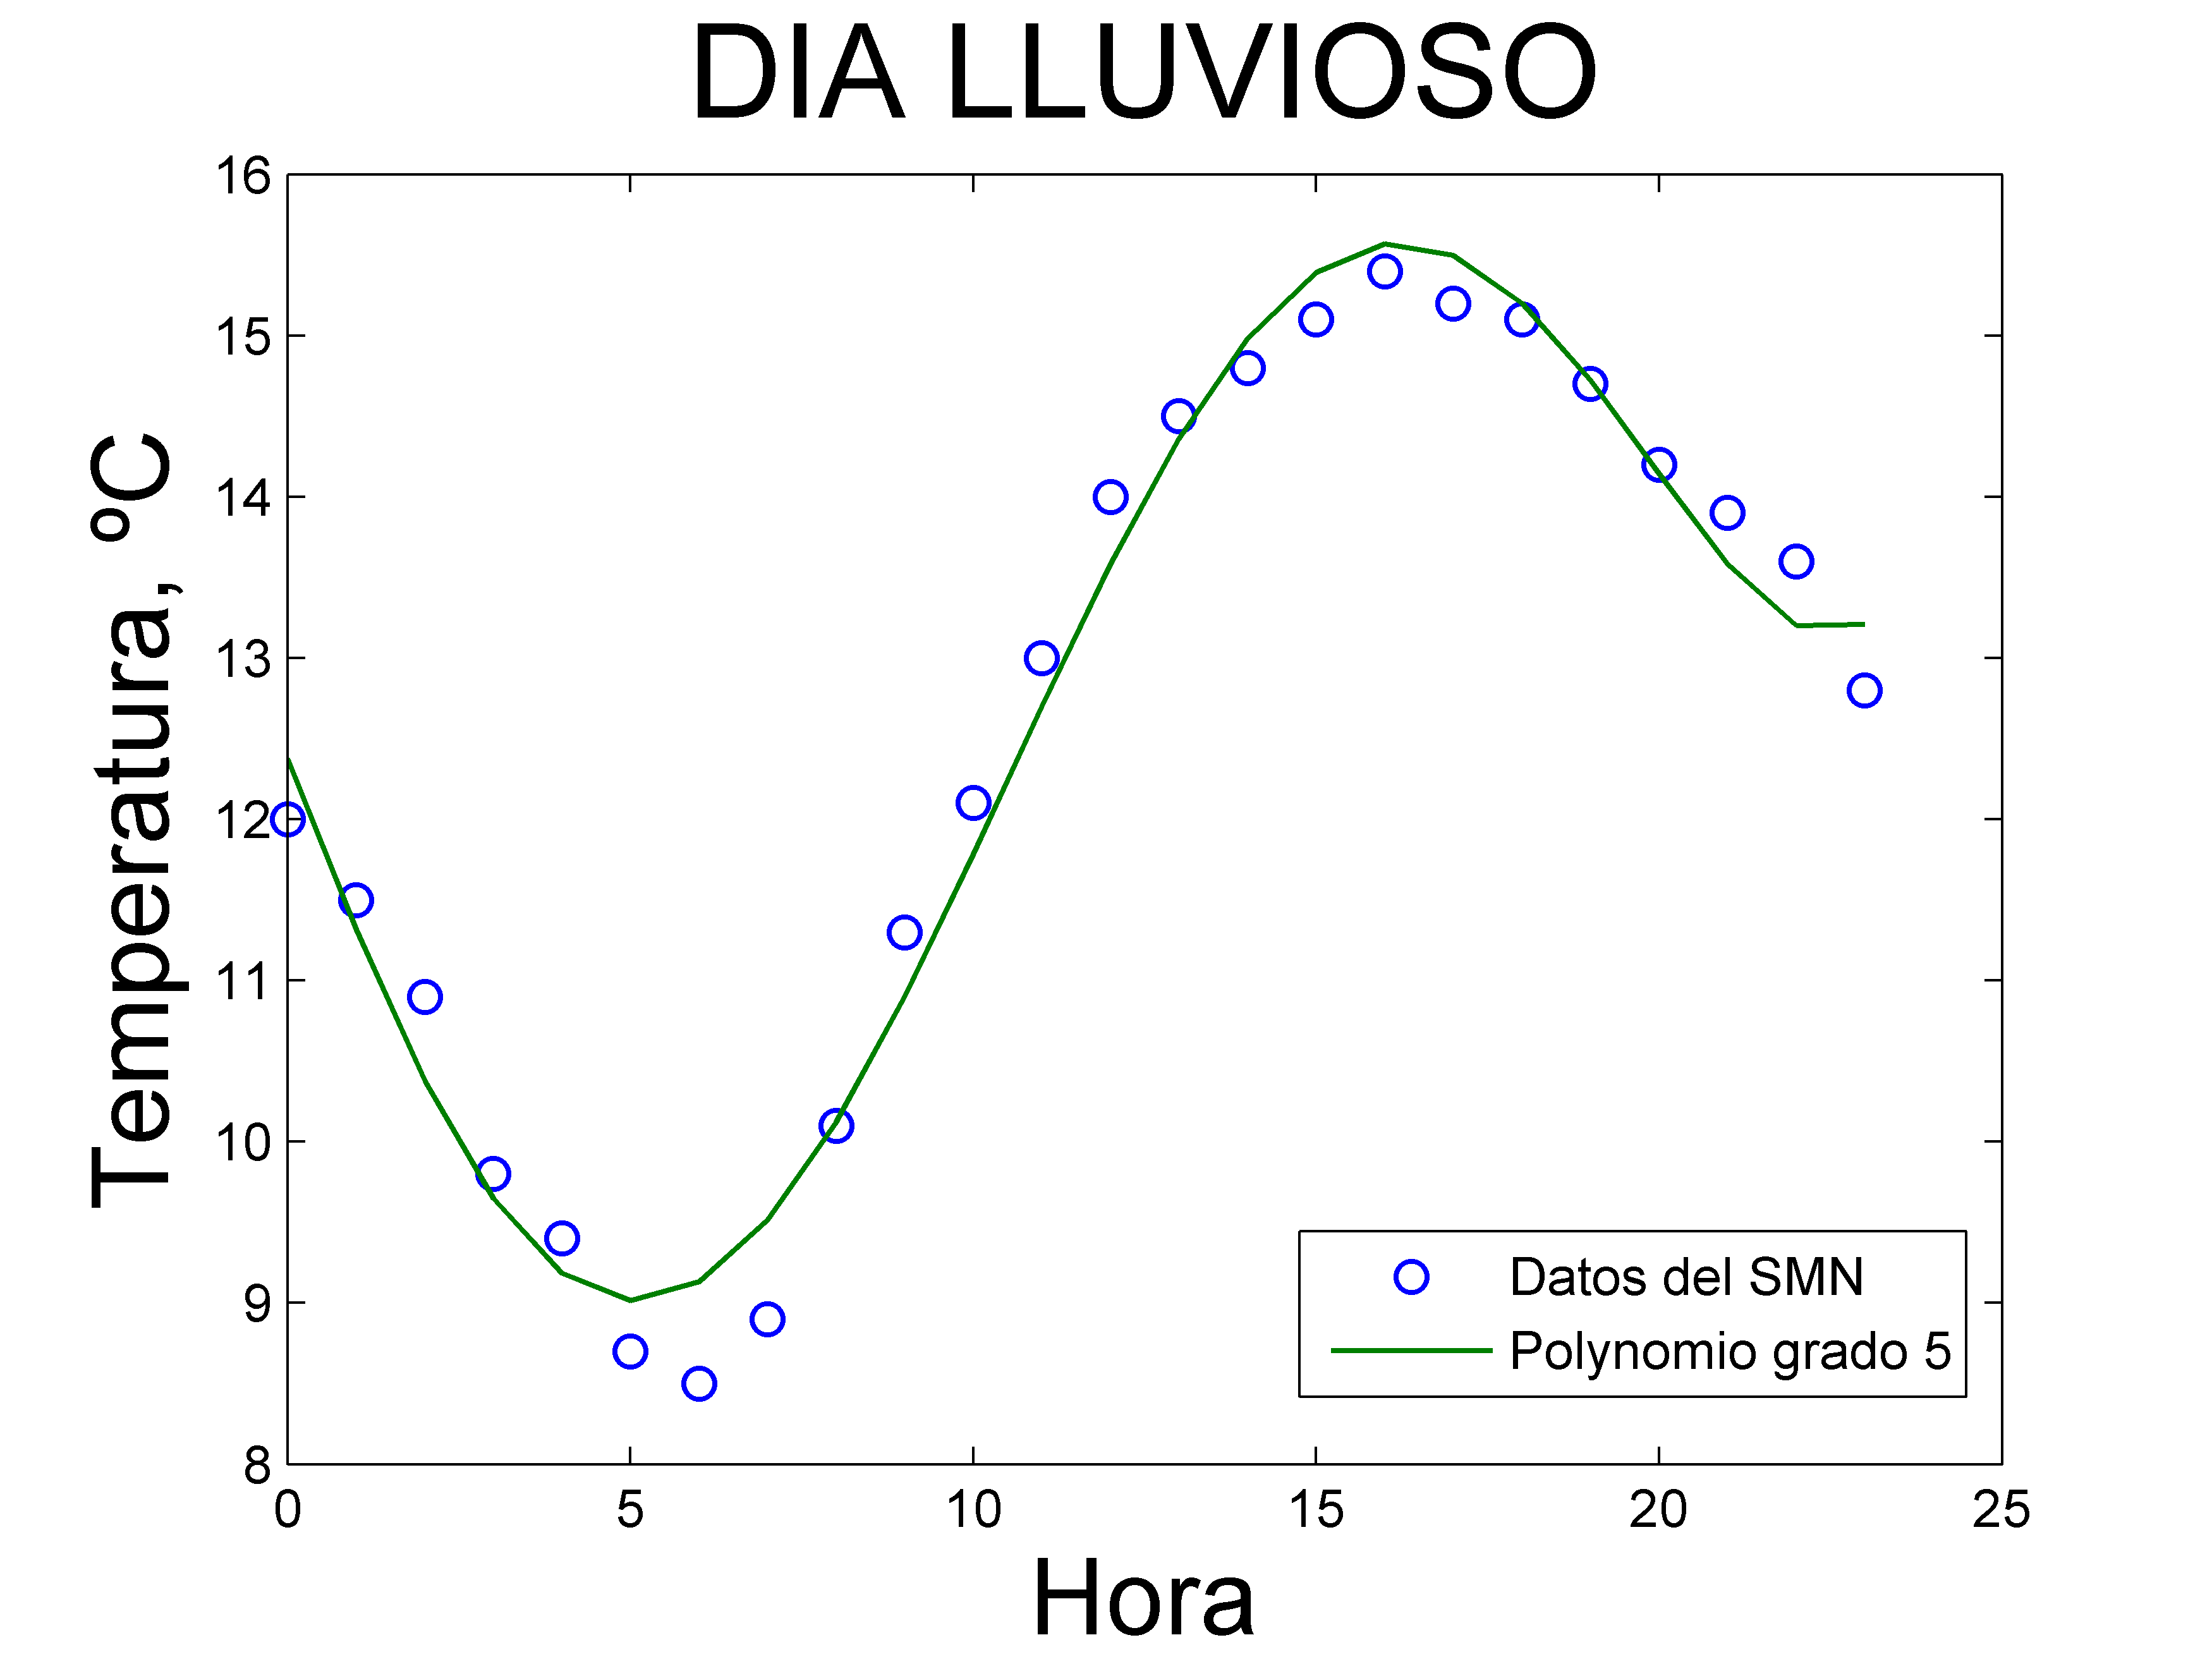
\includegraphics[width=300pt]{./Imagenes/polyfit.png}
\end{center}

\section{Otros comandos}

\begin{enumerate}

\item \textbf{linspace} y \textbf{fplot}: sea la función $f(x)=e^{-x}$, si $-2 \leq x \leq 3$. La gráfica en \textbf{MATLAB} de esta función se obtiene en tres pasos. Primero, mediante el comando \textbf{linspace} se divide el intervalo [-2,3] en 3000 partes. Luego definimos la función y finalmente utilizamos el comando \textbf{plot}.

\begin{lstlisting}[language=Matlab]
>> x=linspace(-2,3,3000);
>> y=exp(-x);
>> plot(x,y);
>> grid on;
\end{lstlisting}
\begin{center}
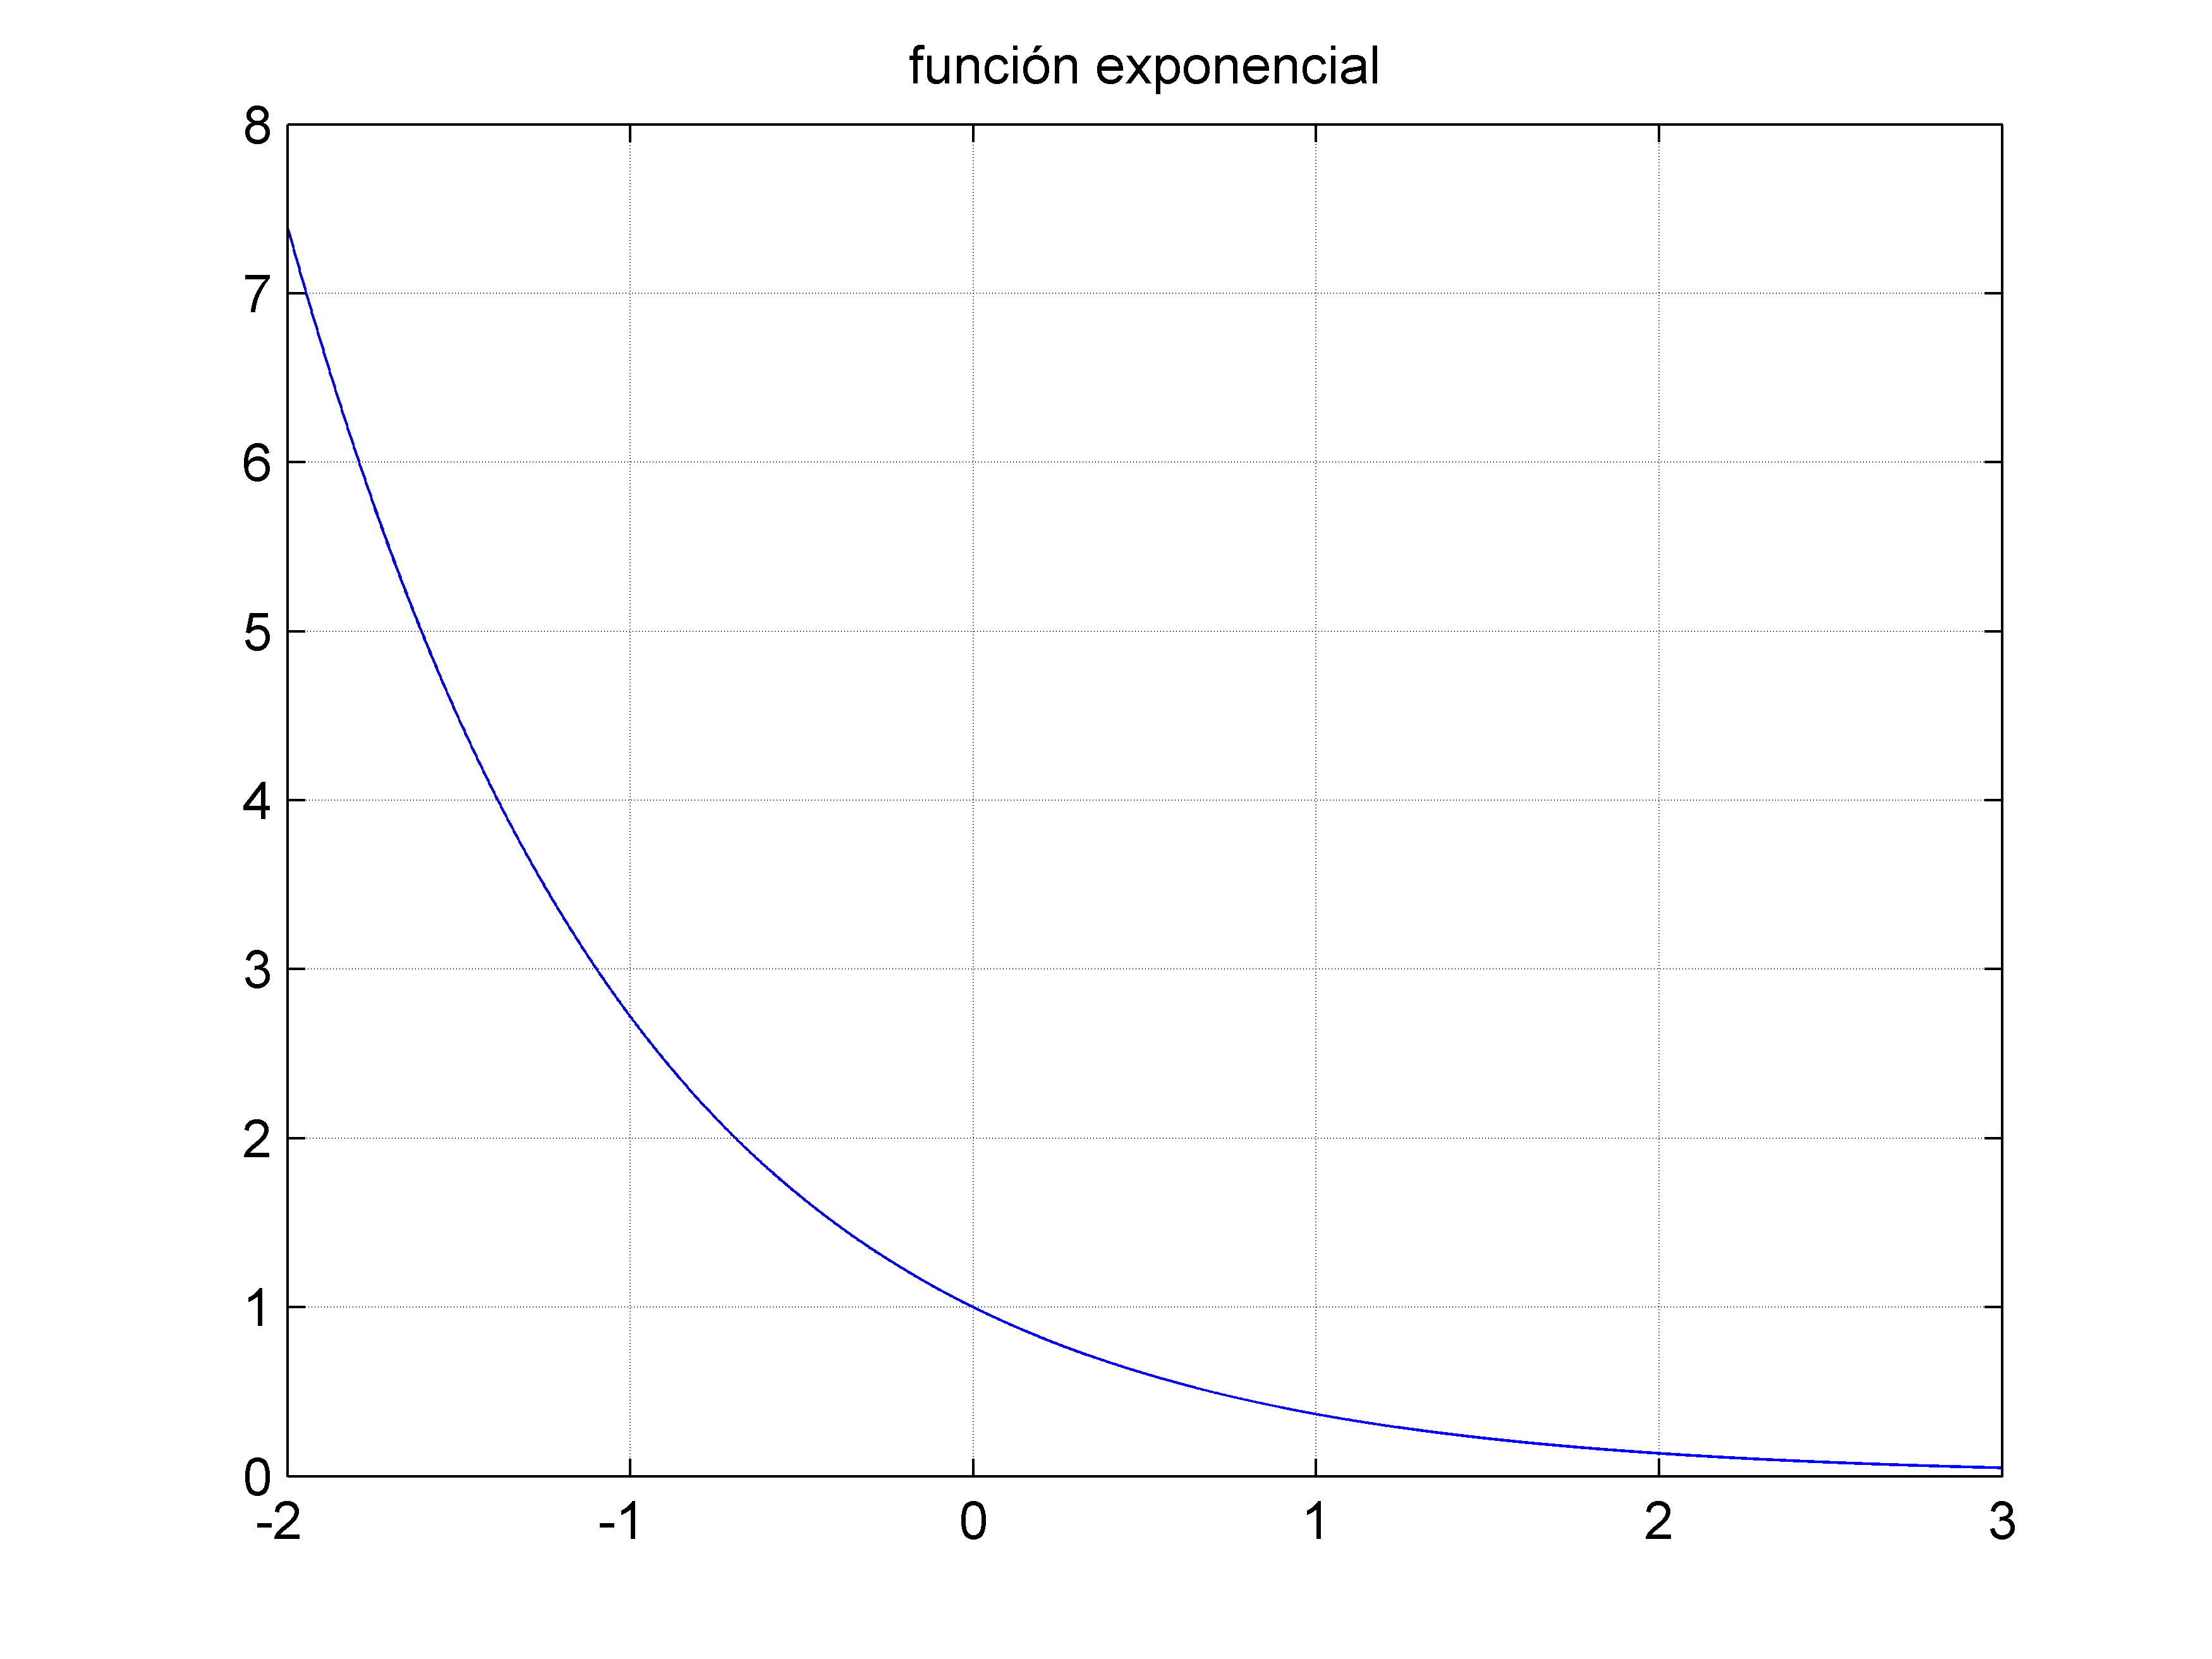
\includegraphics[width=300pt]{./Imagenes/linspace.png}
\end{center} 

Existe otra forma de representar $f$ en un solo paso:
\begin{lstlisting}[language=Matlab]
>> fplot('exp(-x)',[-2,3])
\end{lstlisting}



\item \textbf{Catenaria}: La función que describe esta curva es  $f(x)=cosh(x)$ en el intervalo [-5,5]. Su gráfica se obtiene directamente con la siguiente secuencia de comandos. Primero dividimos el intervalo [-5:5] en pequeños intervalos de 0.1 de longitud. Luego evaluamos $f$ en cada punto \textbf{x} de la división. Finalmente generamos el gráfico.

\begin{lstlisting}[language=Matlab]
>> x=-5:0.1:5;
>> y=cosh(x); 
>> plot(x,y)
\end{lstlisting}
\begin{center}
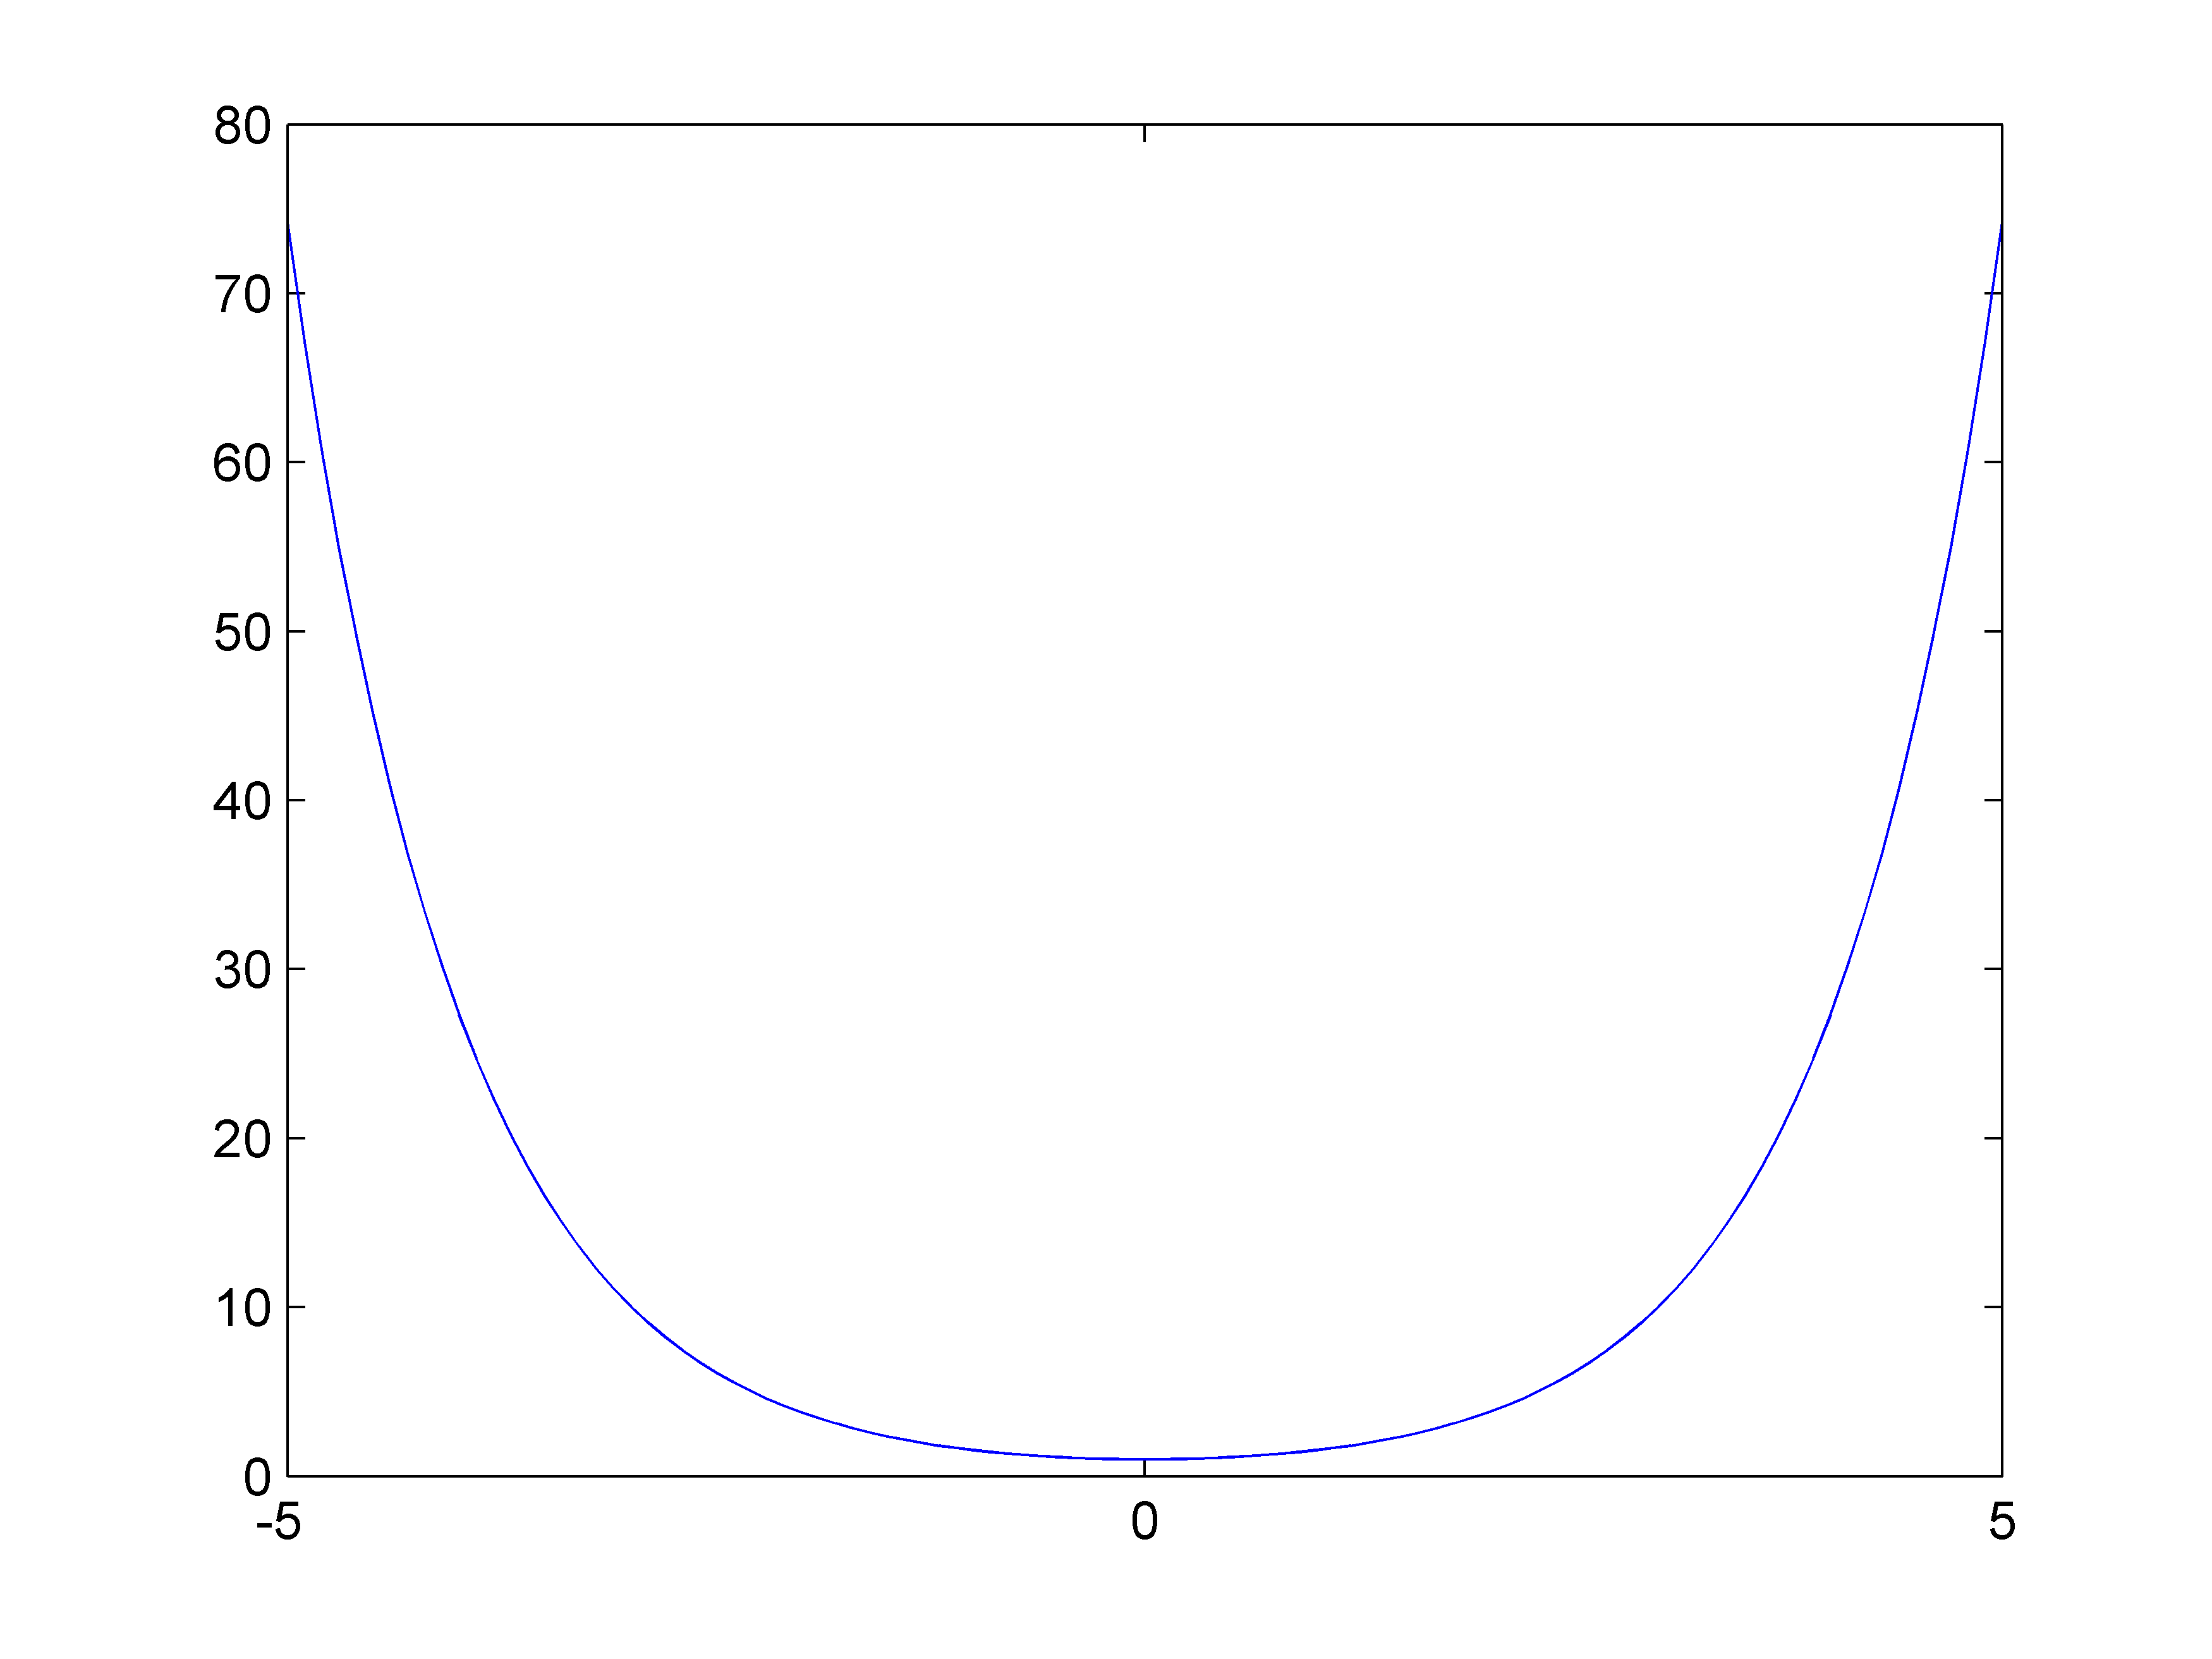
\includegraphics[width=300pt]{./Imagenes/catenaria.png}
\end{center} 


\item Funciones seccionadas usando comandos lógicos. Consideremos la función:

$$
f(n) = \left \{ \begin{matrix} x^{2} & x < 0
\\ 2 & 0 \leqslant x < 1
\\ -x+3 & 1 \leqslant x \end{matrix}\right. 
$$

Para generar el gráfico primero dividimos el intervalo [-2,3] en 3000 partes y luego evaluamos $f$ usando índice lógico:

\begin{lstlisting}[language=Matlab]
>> x=linspace(-2,3,3000);  
>> y=(x.^2).*(x<0)+2.*((0<=x)&(x<1))+(-x+3).*(1<=x); 
>> plot(x,y)
\end{lstlisting}
\begin{center}
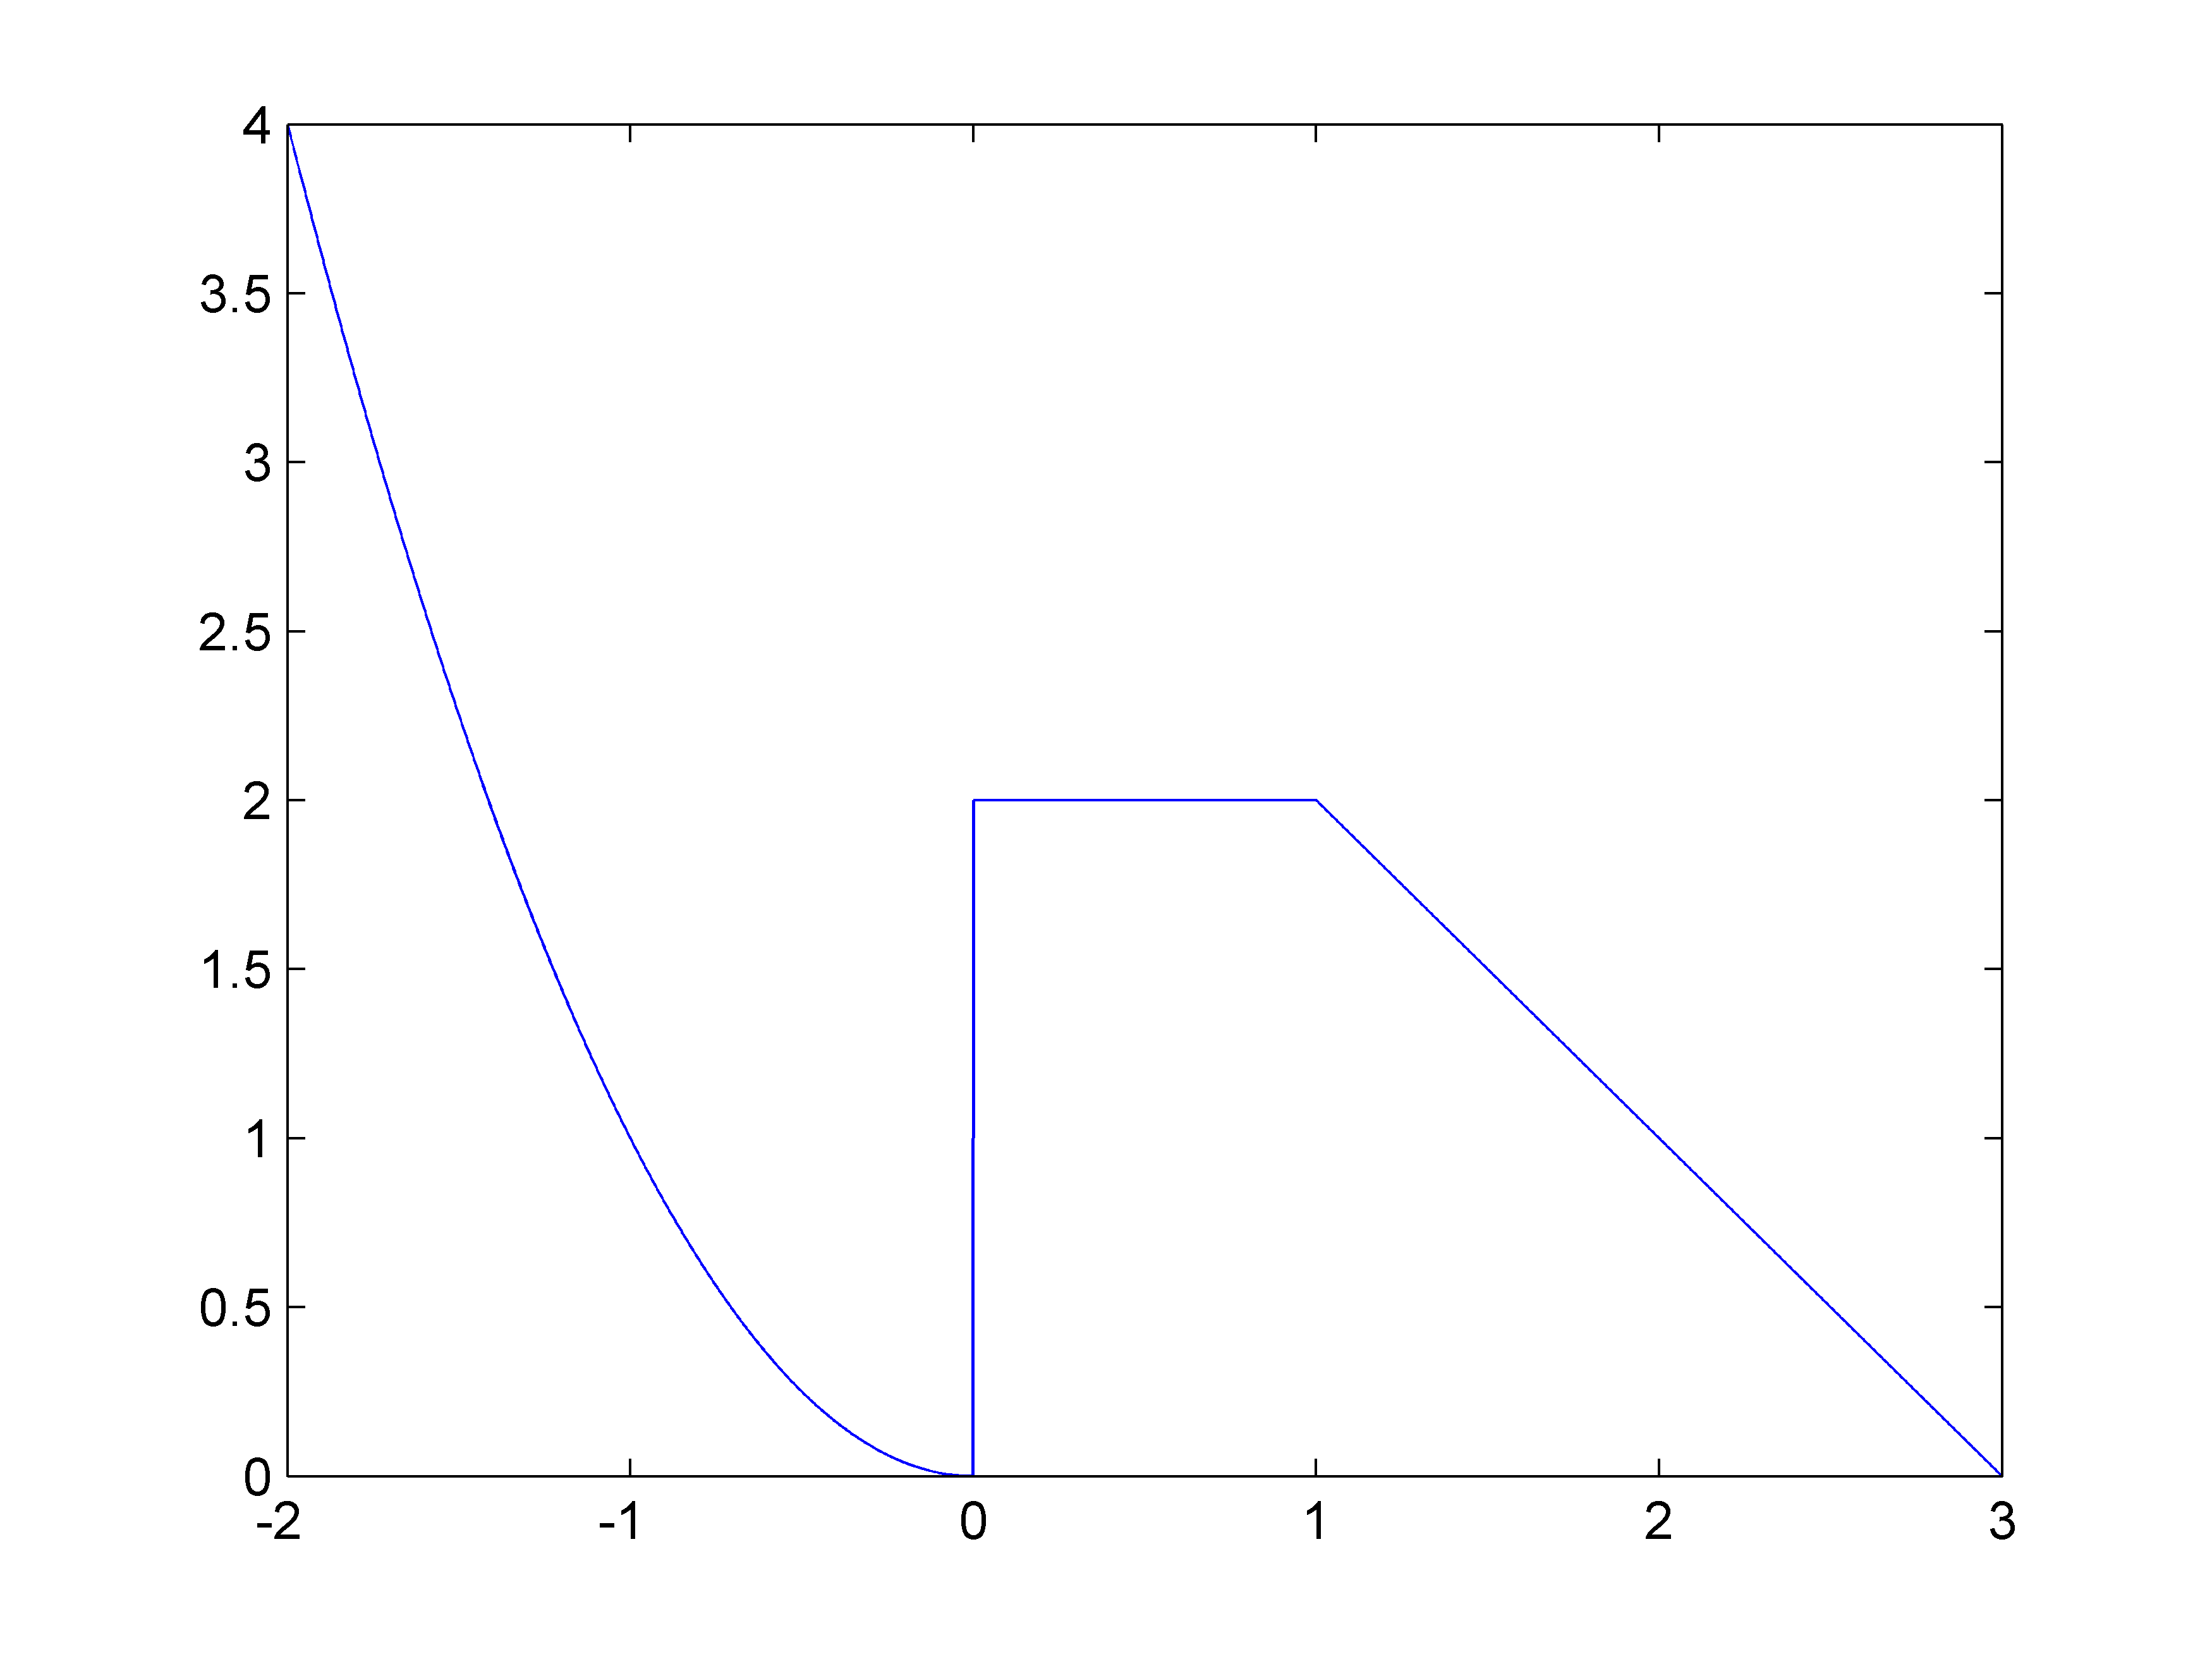
\includegraphics[width=300pt]{./Imagenes/variasf.png}
\end{center} 

\end{enumerate}

\section{Curvas en coordenadas paramétricas}
 
Sea $F(x,y)=0$ con \textbf{x} e \textbf{y} reales, la ecuación cartesiana de una curva C. Si tanto \textbf{x} como \textbf{y} son funciones de una tercera variable \textbf{t}, $t \in I=[a,b]$ , entonces la curva queda representada por

$$
C : \left \{ \begin{matrix} x = x(t)
\\ y = y(t)' \end{matrix}\right. 
$$

denominadas ecuaciones paramétricas de \textbf{C} y \textbf{t} el parámetro. Para cada valor de \textbf{t}, las ecuaciones paramétricas determinan valores correspondientes de \textbf{x} y de 
\textbf{y}, siendo \textbf{(x;y)} un punto de la curva.

\begin{enumerate}

\item Sea la curva con ecuaciones paramétricas:
$$
C : \left \{ \begin{matrix} x(t) = 4cos(t) - cos(4t) & t \in [0,2\pi]
\\ y(t) = 4sen(t) - sen(4t) \end{matrix}\right. 
$$
\begin{lstlisting}[language=Matlab]
>> t=0:0.1:2*pi; 
>> x=4*cos(t)-cos(4*t);  
>> y=4*sin(t)-sin(4*t);  
>> plot(x,y)
\end{lstlisting}
\begin{center}
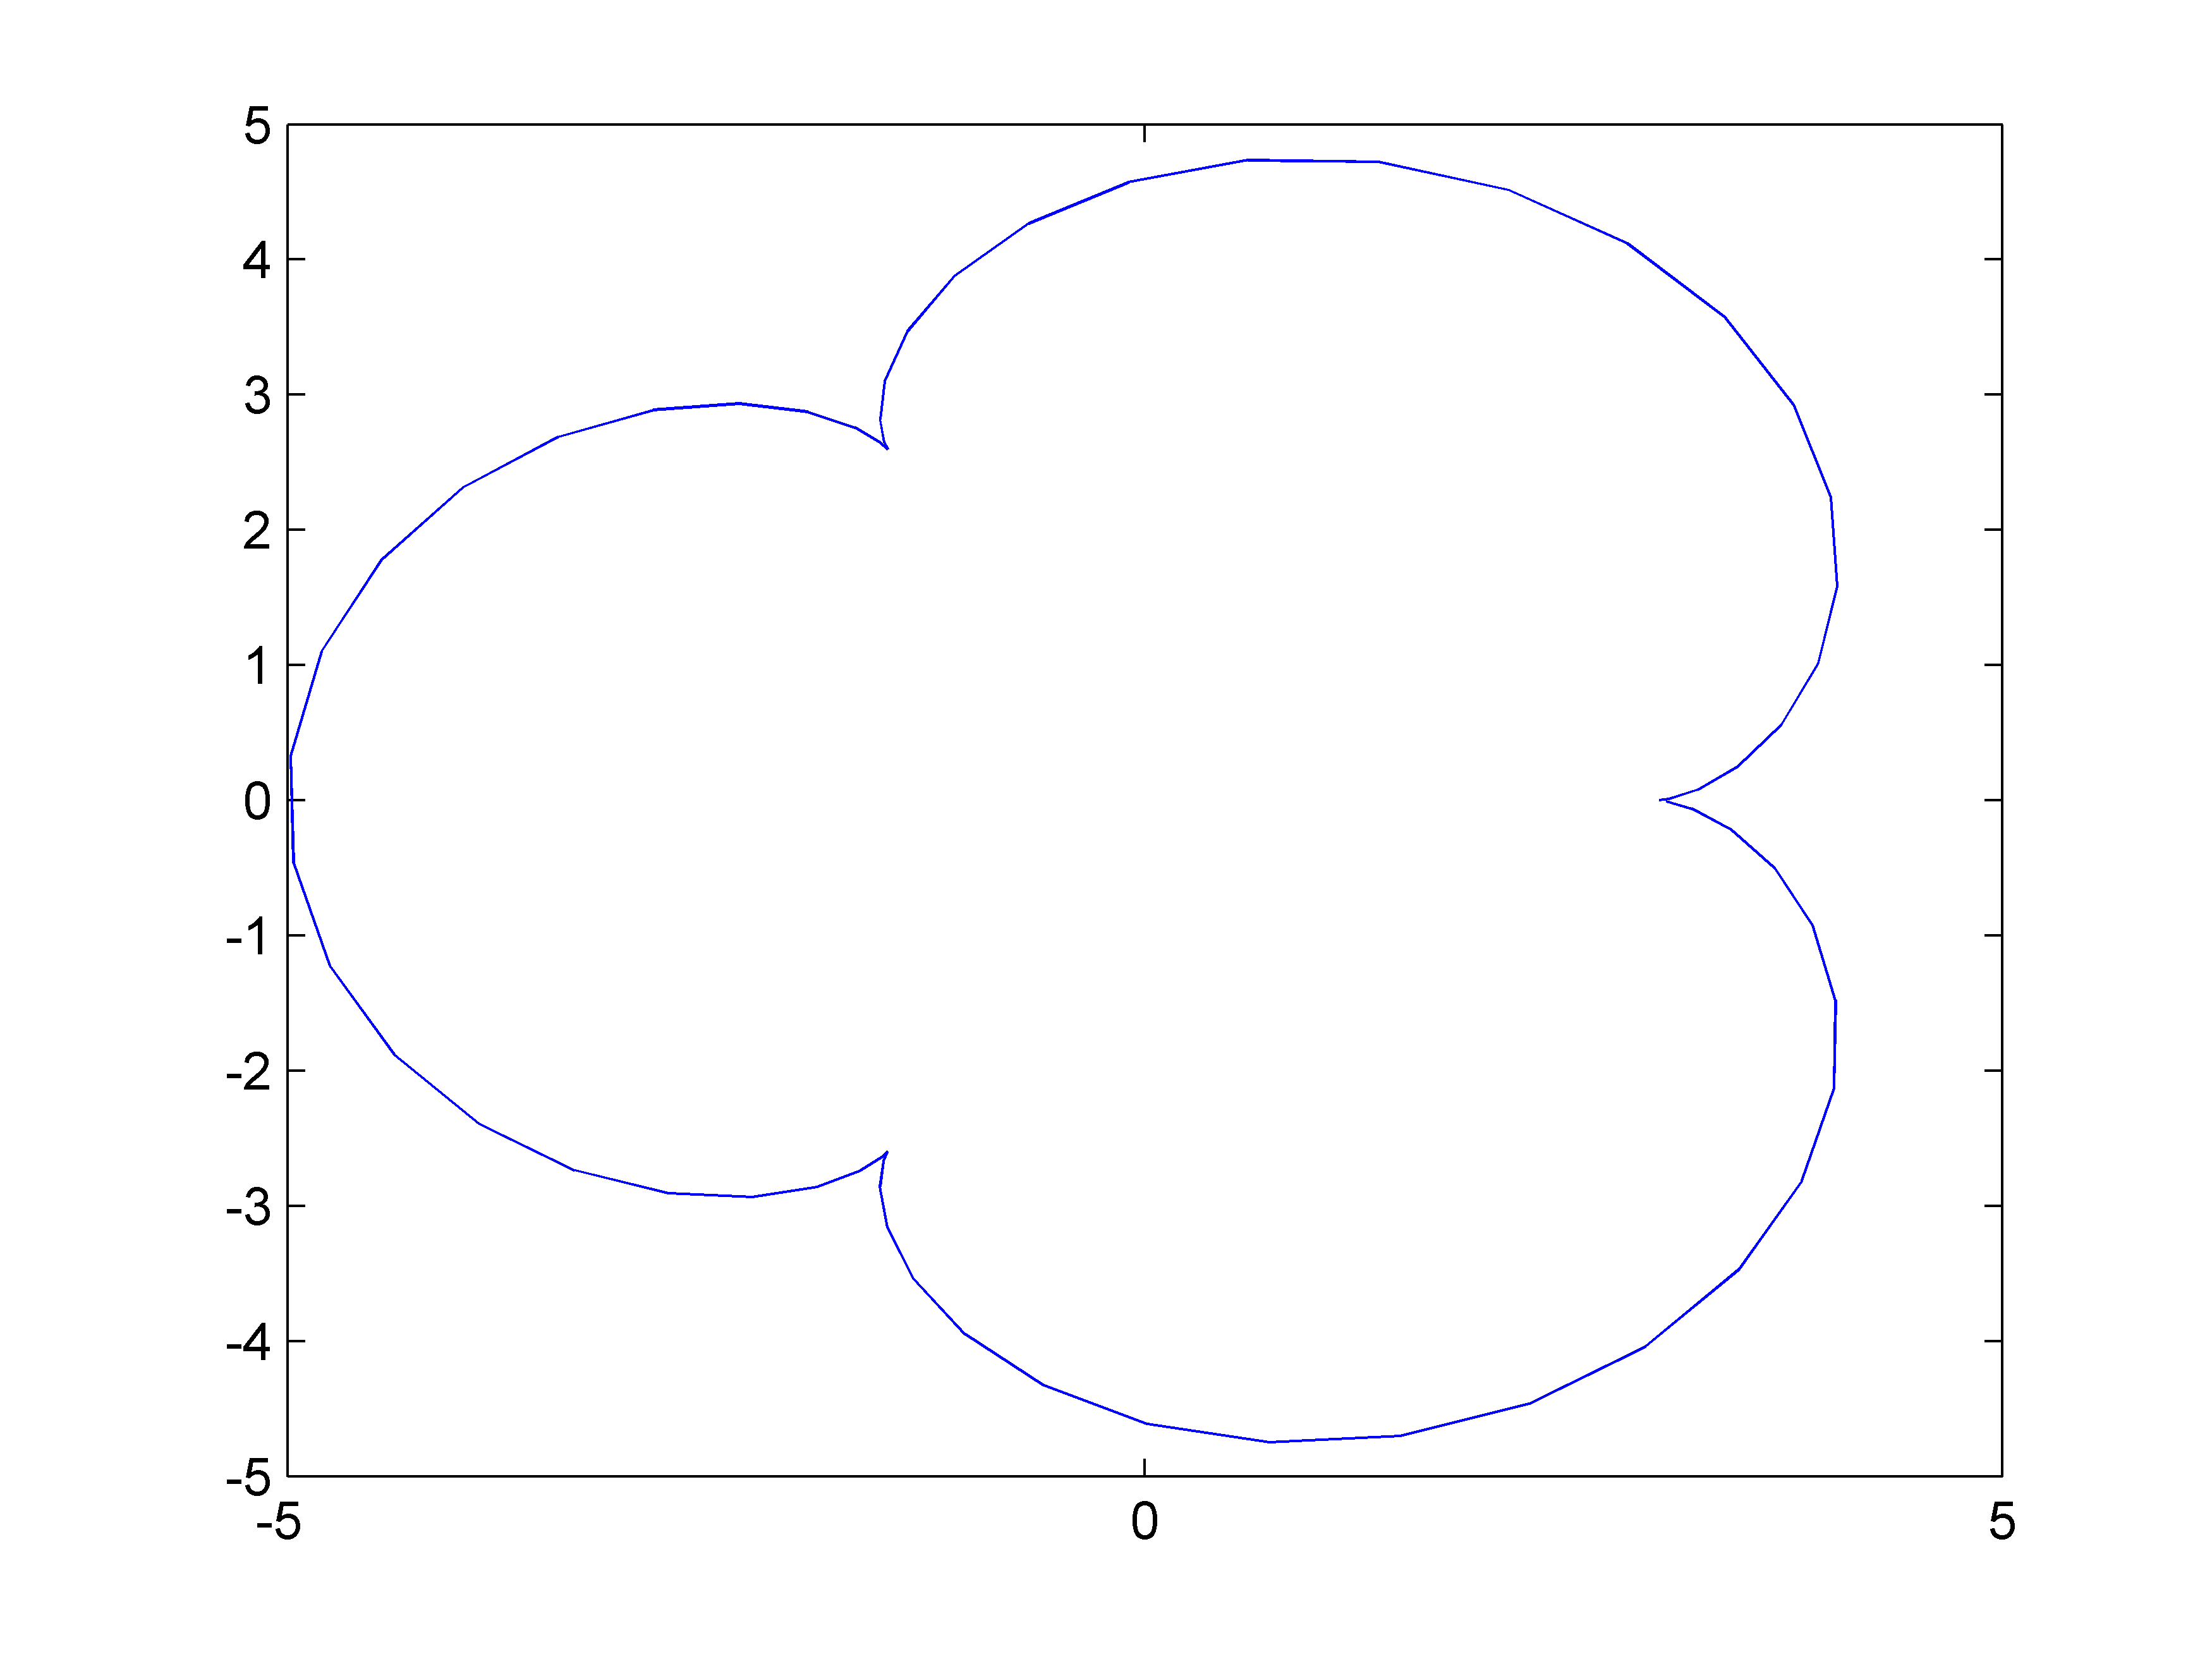
\includegraphics[width=300pt]{./Imagenes/param1.png}
\end{center}

\item Sea C la semicircunferencia unitaria con ecuaciones paramétricas:
$$
C : \left \{ \begin{matrix} x(t) = cos(t) & t \in [0,\pi]
\\ y(t) = sen(t) \end{matrix}\right. 
$$
\begin{lstlisting}[language=Matlab]
>> t=linspace(0,pi,30); 
>> plot(cos(t),sin(t))
\end{lstlisting}
\begin{center}
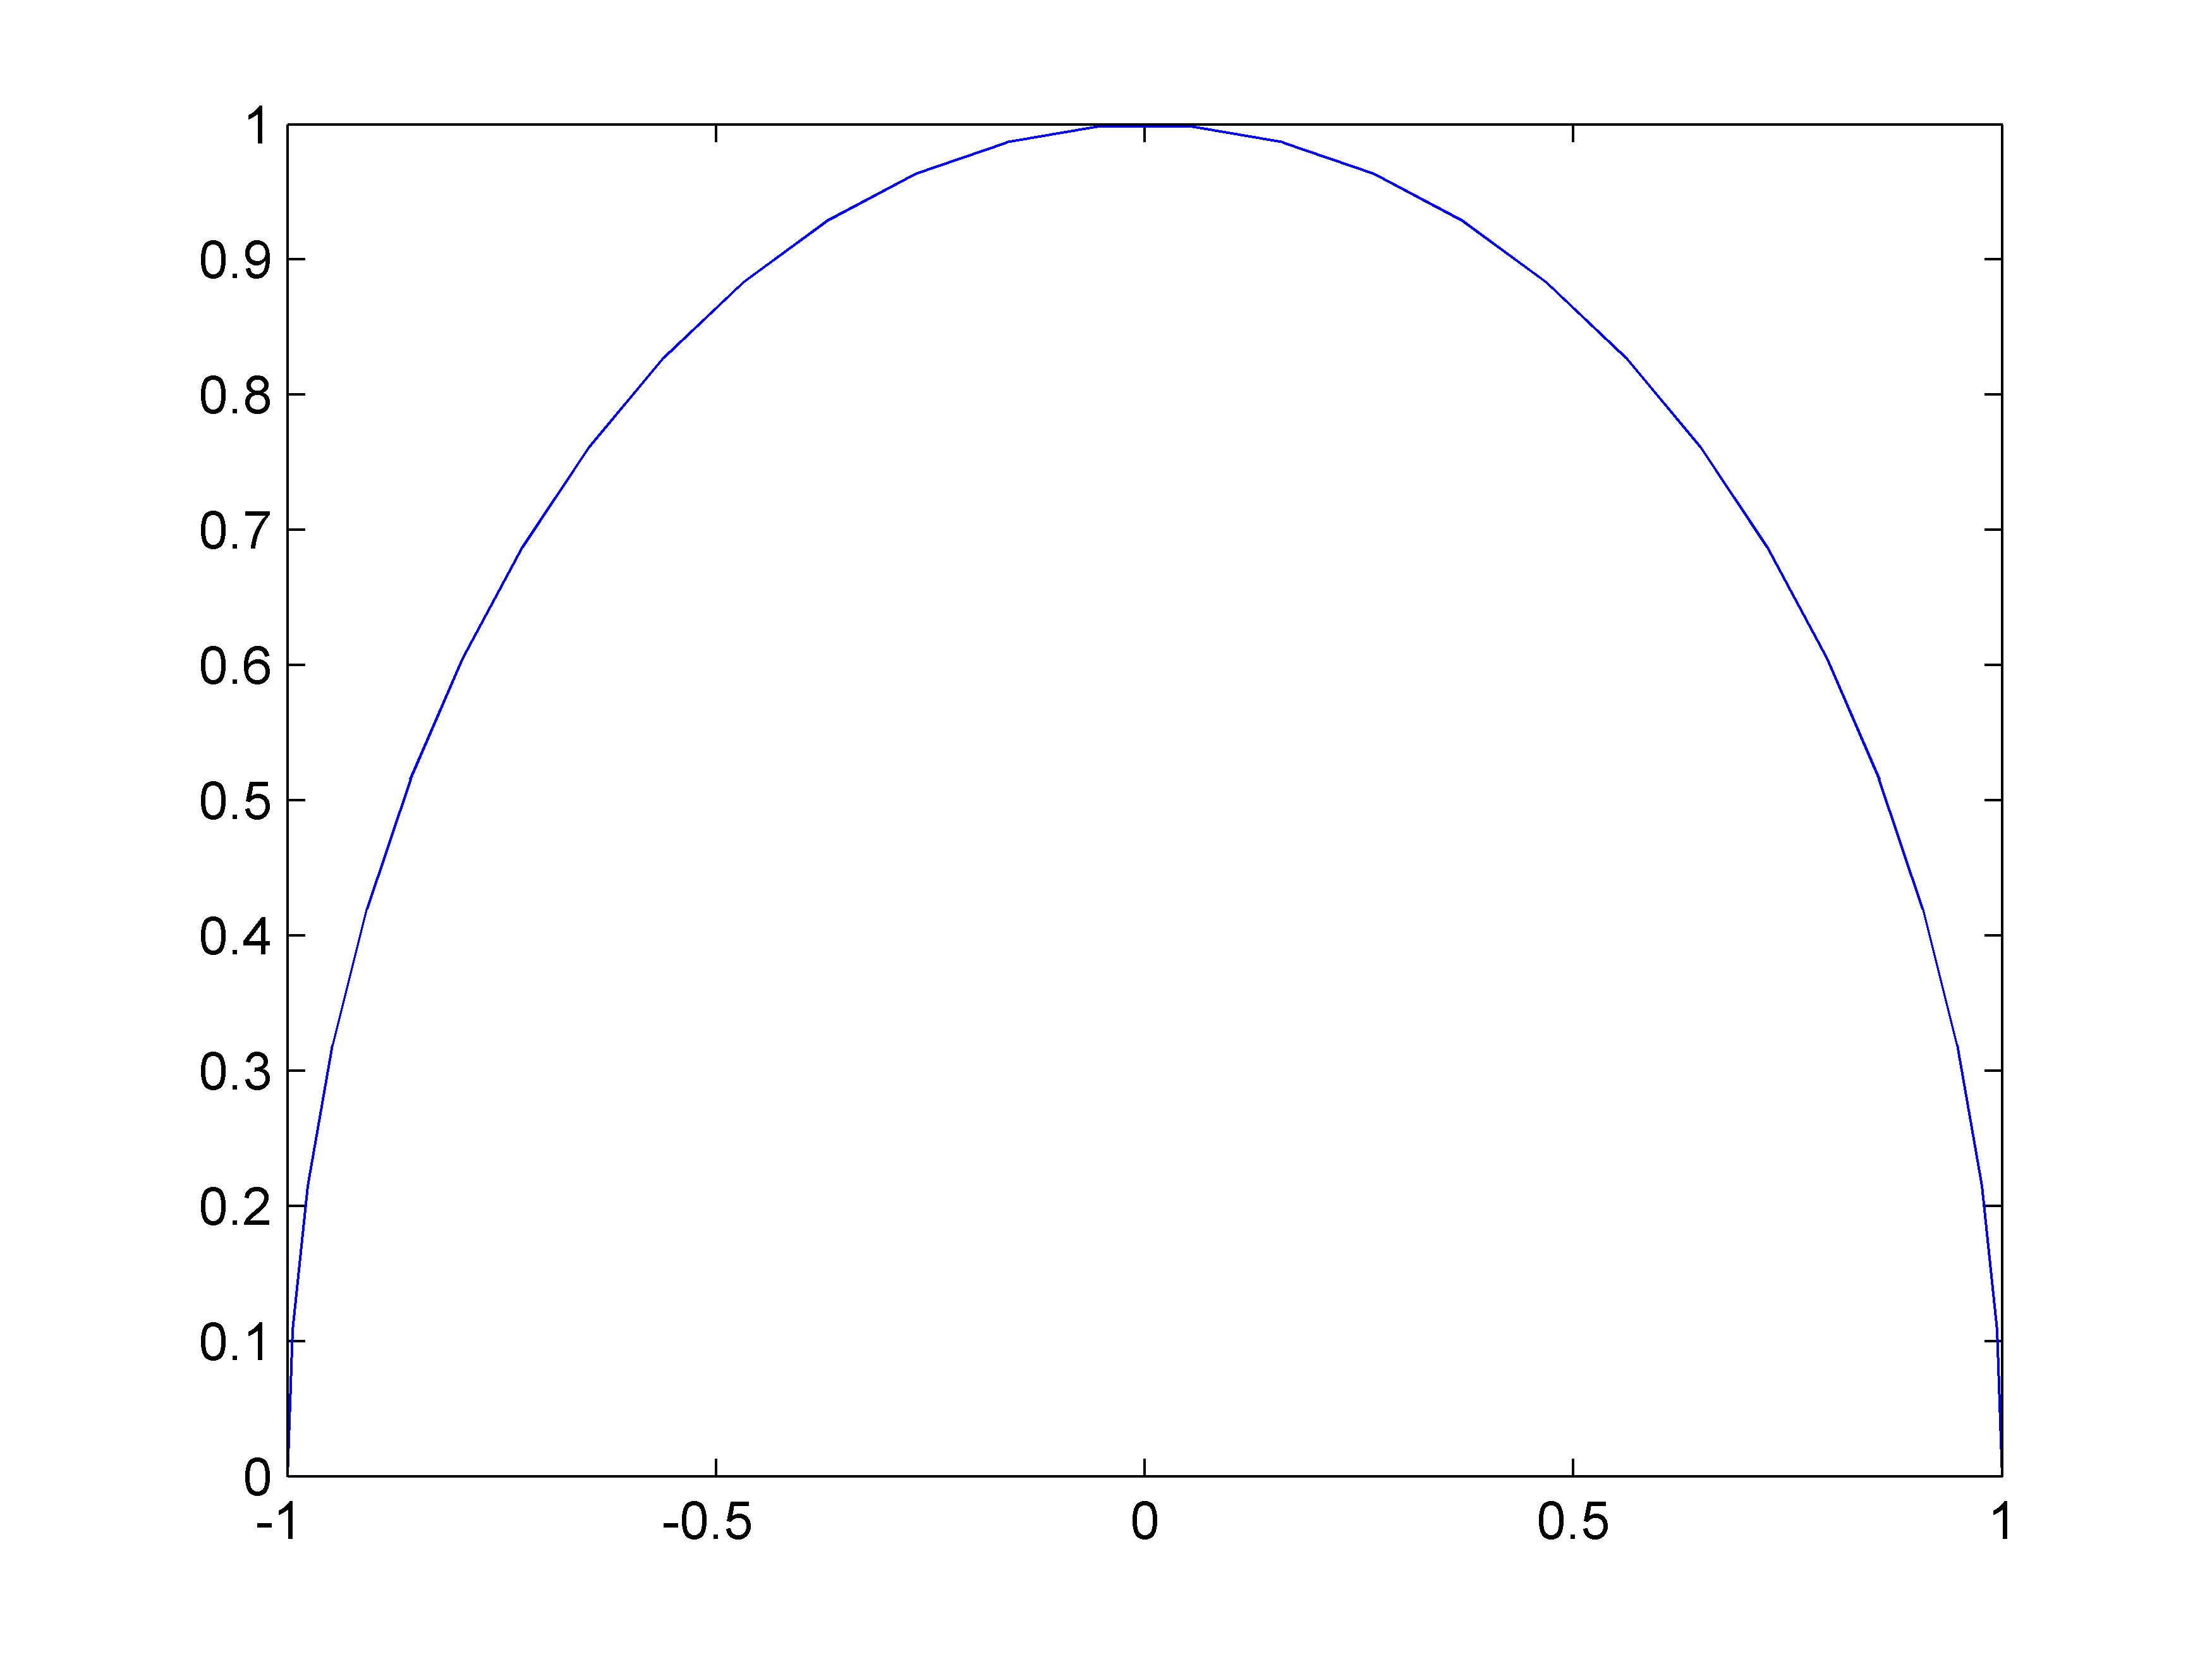
\includegraphics[width=300pt]{./Imagenes/param2.png}
\end{center} 


\item Vectores tangentes a la semicircunferencia anterior en 10 puntos de la curva. A la semicircunferencia anterior le adicionamos los vectores tangentes de la siguiente forma:
\begin{lstlisting}[language=Matlab]
>> t=linspace(0,pi,30); 
>> plot(cos(t),sin(t));
>> hold on  
>> t=linspace(0,pi,10); 
>> quiver(cos(t),sin(t),-sin(t),cos(t)
\end{lstlisting}
\begin{center}
\includegraphics[width=300pt]{./Imagenes/param3.png}
\end{center} 
\end{enumerate}

\section{Curvas en coordenadas polares}

Las coordenadas polares de un punto \textbf{P} las denotaremos por $(r,\theta)$, donde $r$ representa el radio vector y $\theta$ el ángulo polar. Ejemplos:

\begin{enumerate}

\item \textbf{Cardioide}: Ecuación $ r = 1+cos(\theta) donde 0 \leqslant \theta \leqslant 2\pi$. Directamente en la ventana de comandos escribimos:

\begin{lstlisting}[language=Matlab]
>> teta=linspace(0,2*pi,60);
>> r=1+cos(teta);
>> polar(teta,r)
\end{lstlisting}
\begin{center}
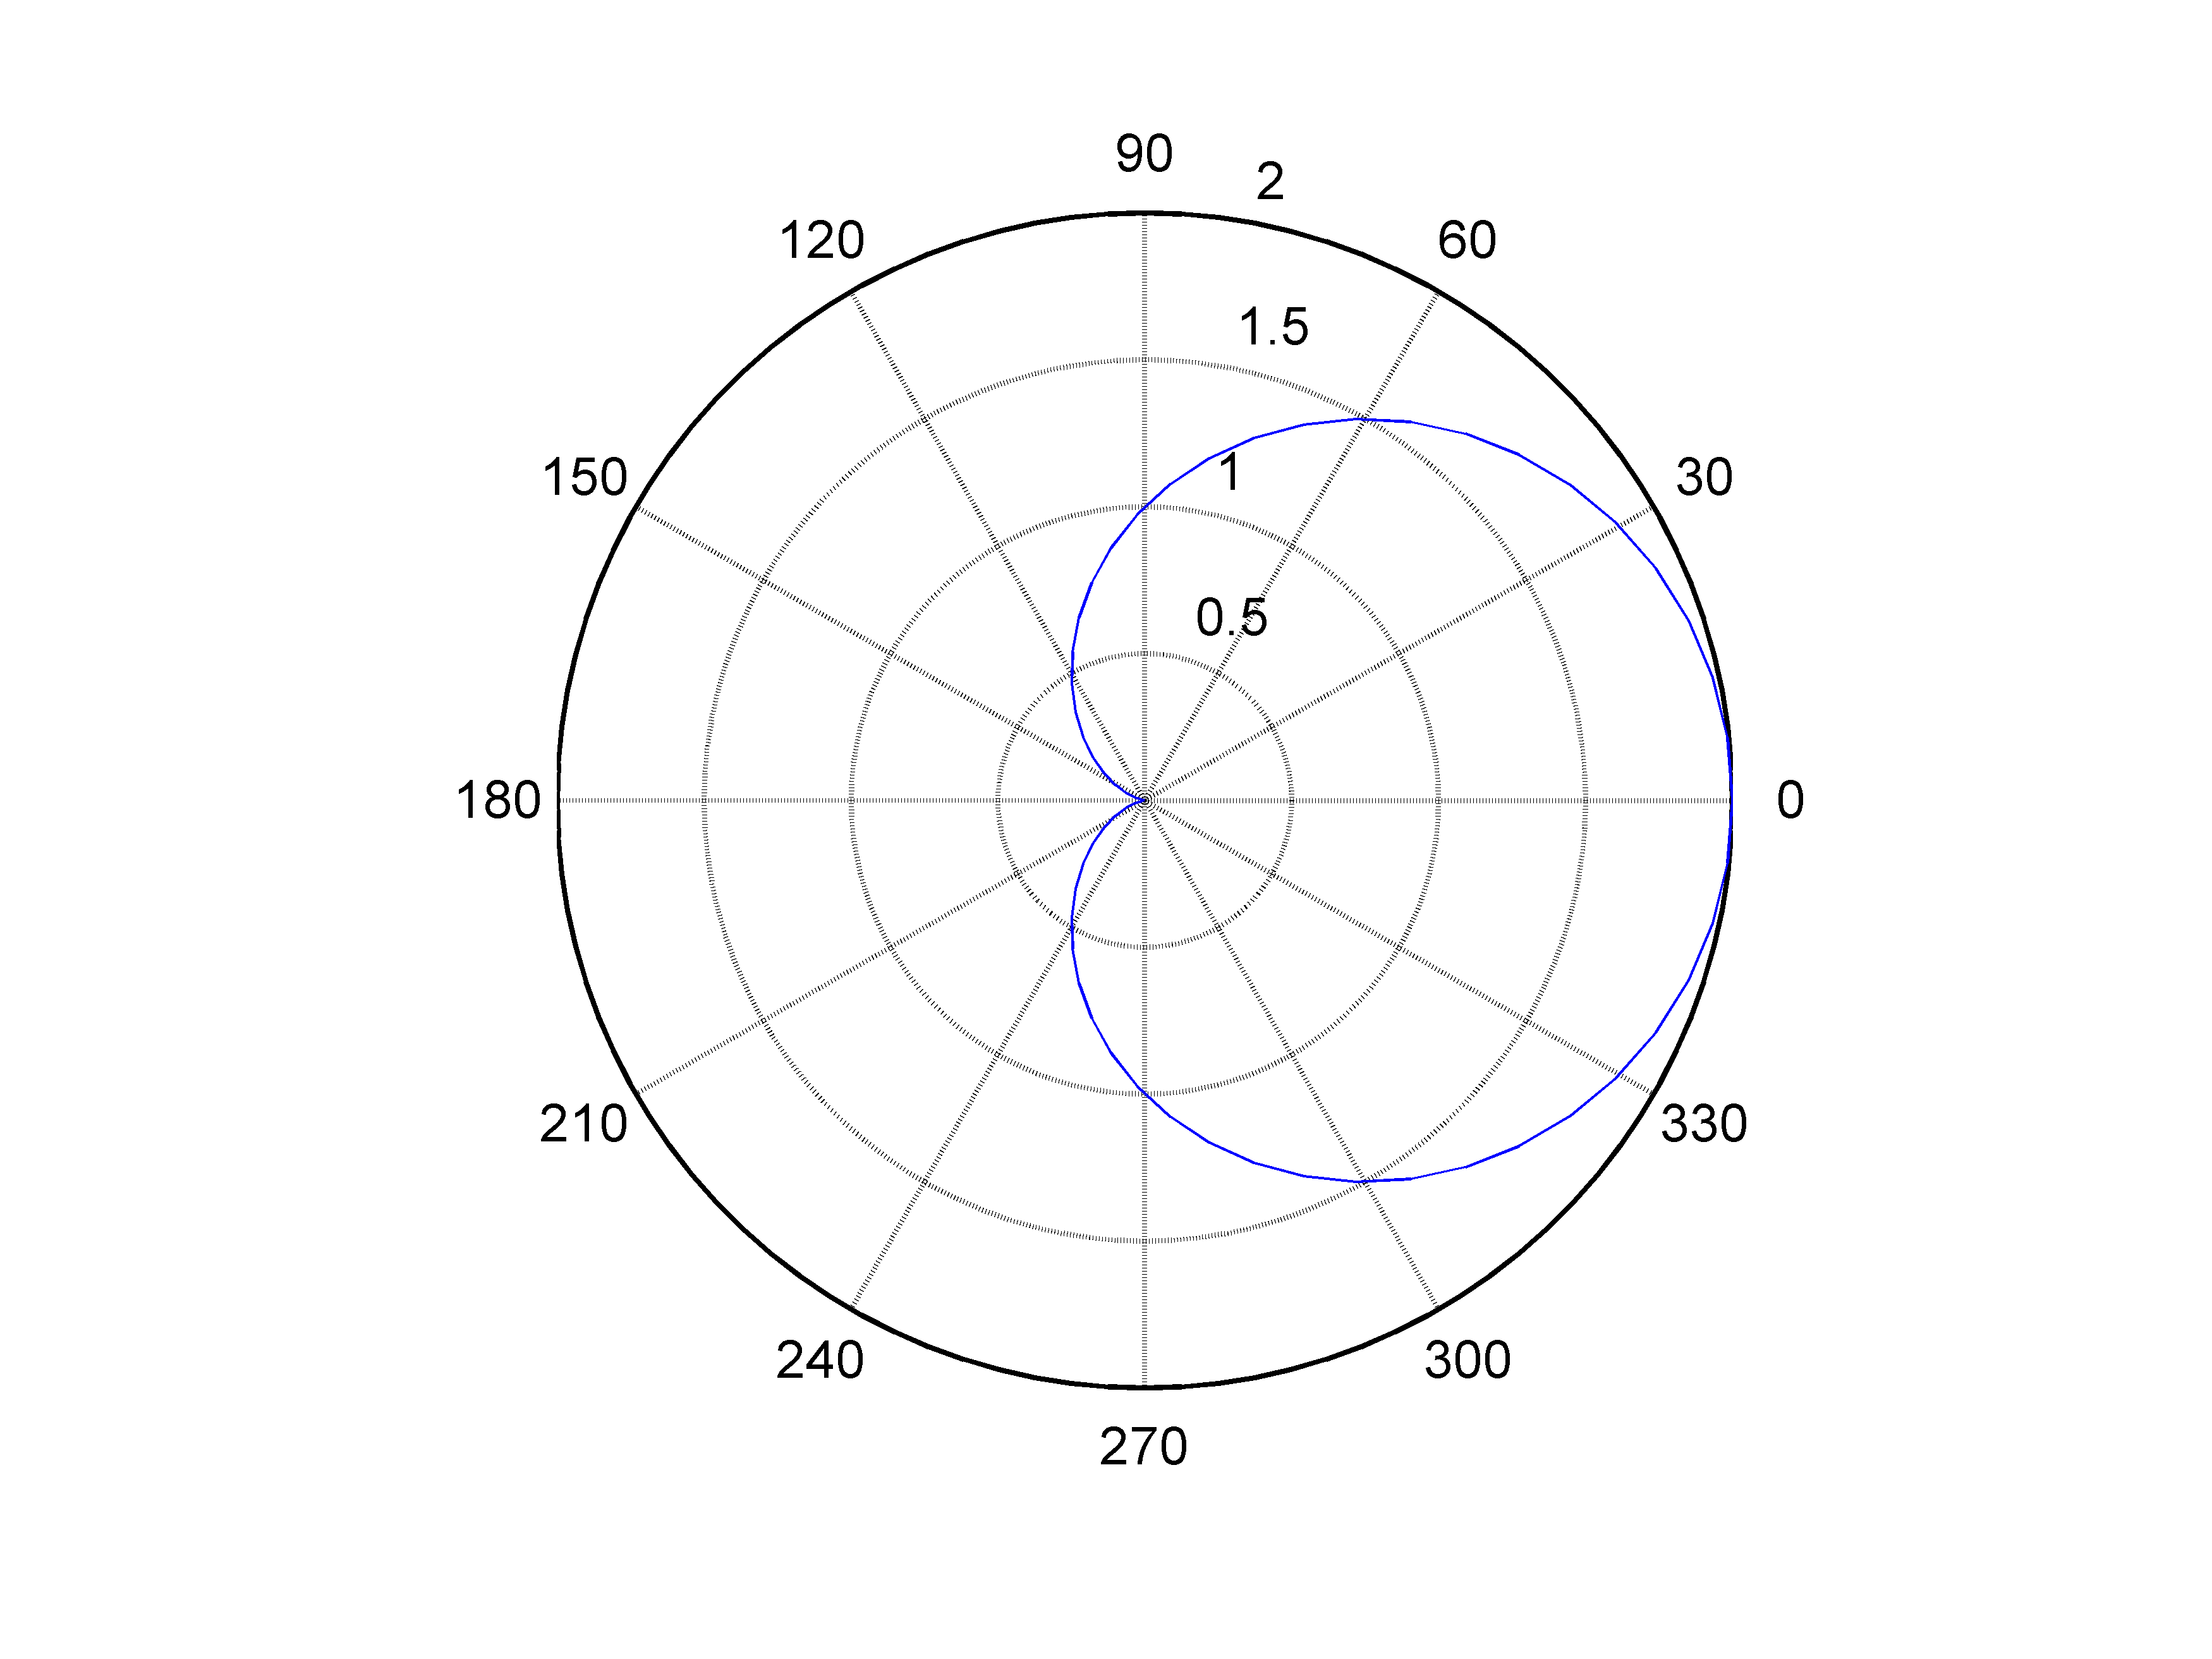
\includegraphics[width=300pt]{./Imagenes/polar1.png}
\end{center} 
 

\item 2. \textbf{Lemniscata de Bernoulli}: de ecuación $r^{2} = 4cos(2\theta), 0 \leqslant \theta \leq 2\pi$. 
La grafica se obtiene mediante los siguientes comandos:

\begin{lstlisting}[language=Matlab]
>> theta=linspace(0,2*pi,300); 
>> r=sqrt(4*cos(2*theta)); 
>> polar(theta,r)
\end{lstlisting}
\begin{center}
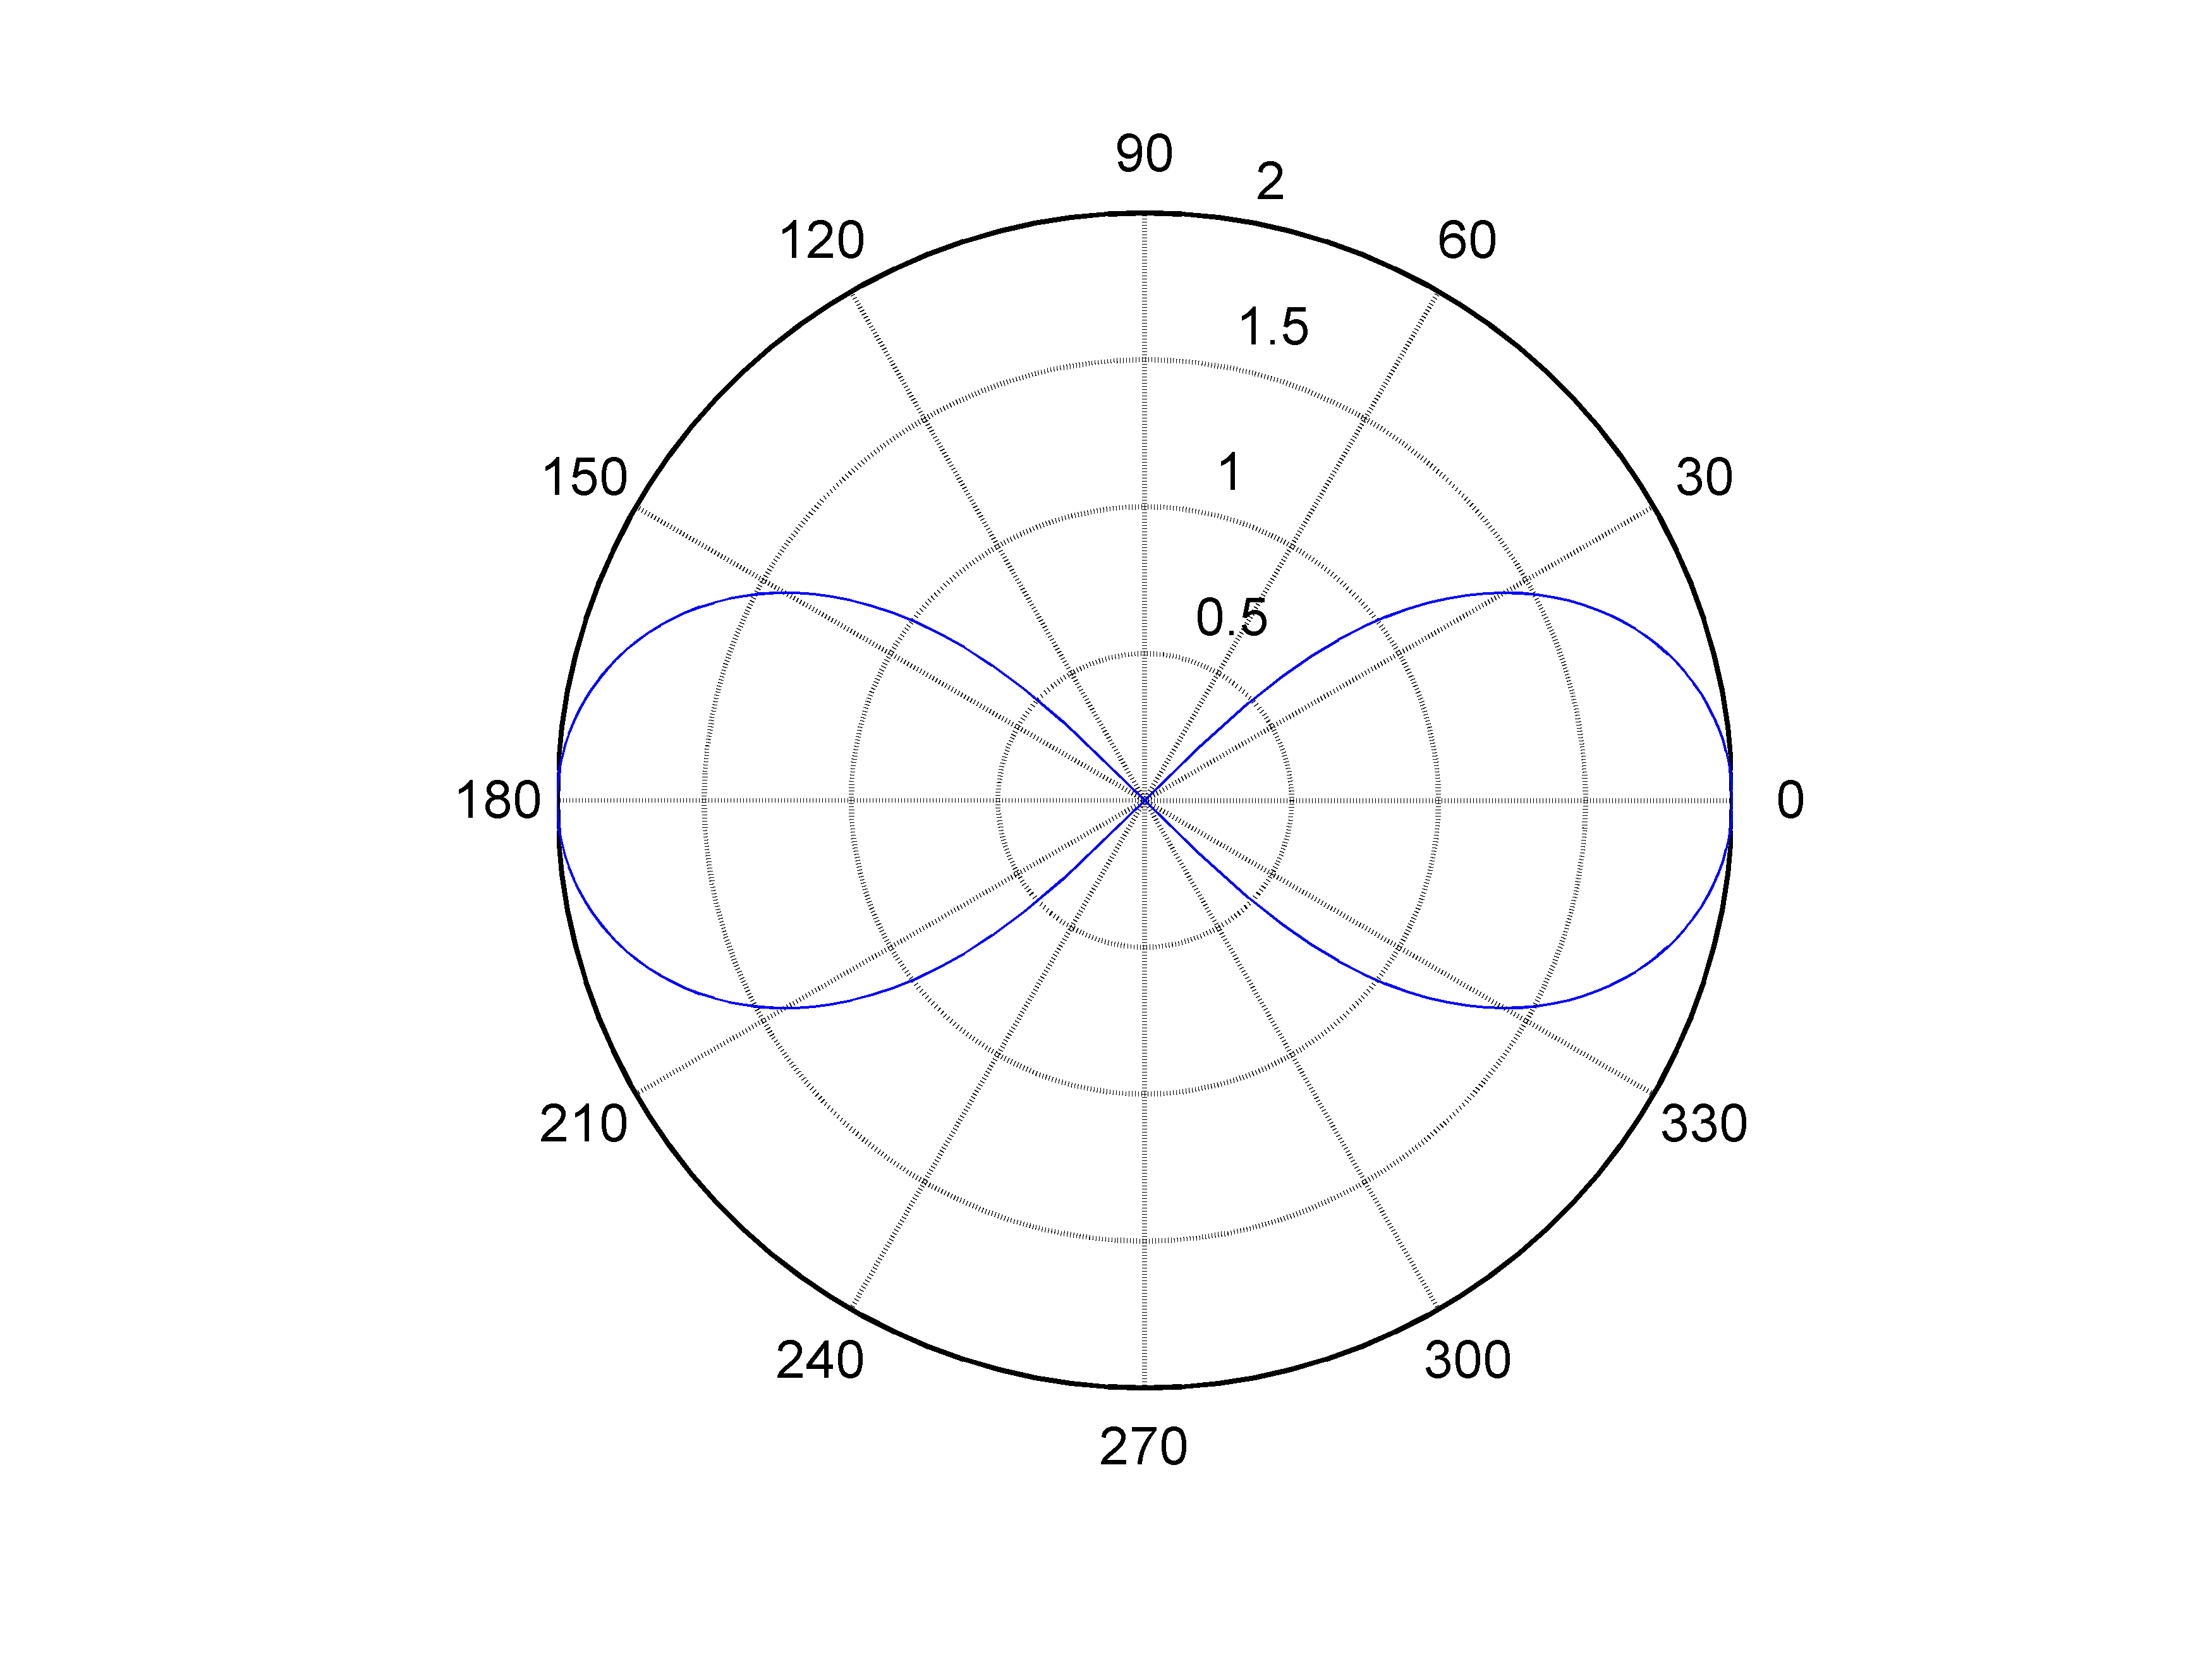
\includegraphics[width=300pt]{./Imagenes/polar2.png}
\end{center} 

\end{enumerate}
\chapter{Campos vectoriales}

Los comandos usados para representar campos vectoriales son \textbf{quiver} y \textbf{quiver3}, que son respectivamente para 2D y 3D. Básicamente, a cada punto se le asigna un vector y se lo representa. Veamos un ejemplo:

\begin{lstlisting}[language=Matlab]
>> [X,Y] = meshgrid(-2:.15:2,-2:.15:2);
>> Z = X.*exp(-X.^2-Y.^2);
>> [px,py] = gradient(Z,.15,.15);
>> contour(X,Y,Z), hold on, quiver(X,Y,px,py), colorbar
>> hold off
\end{lstlisting}

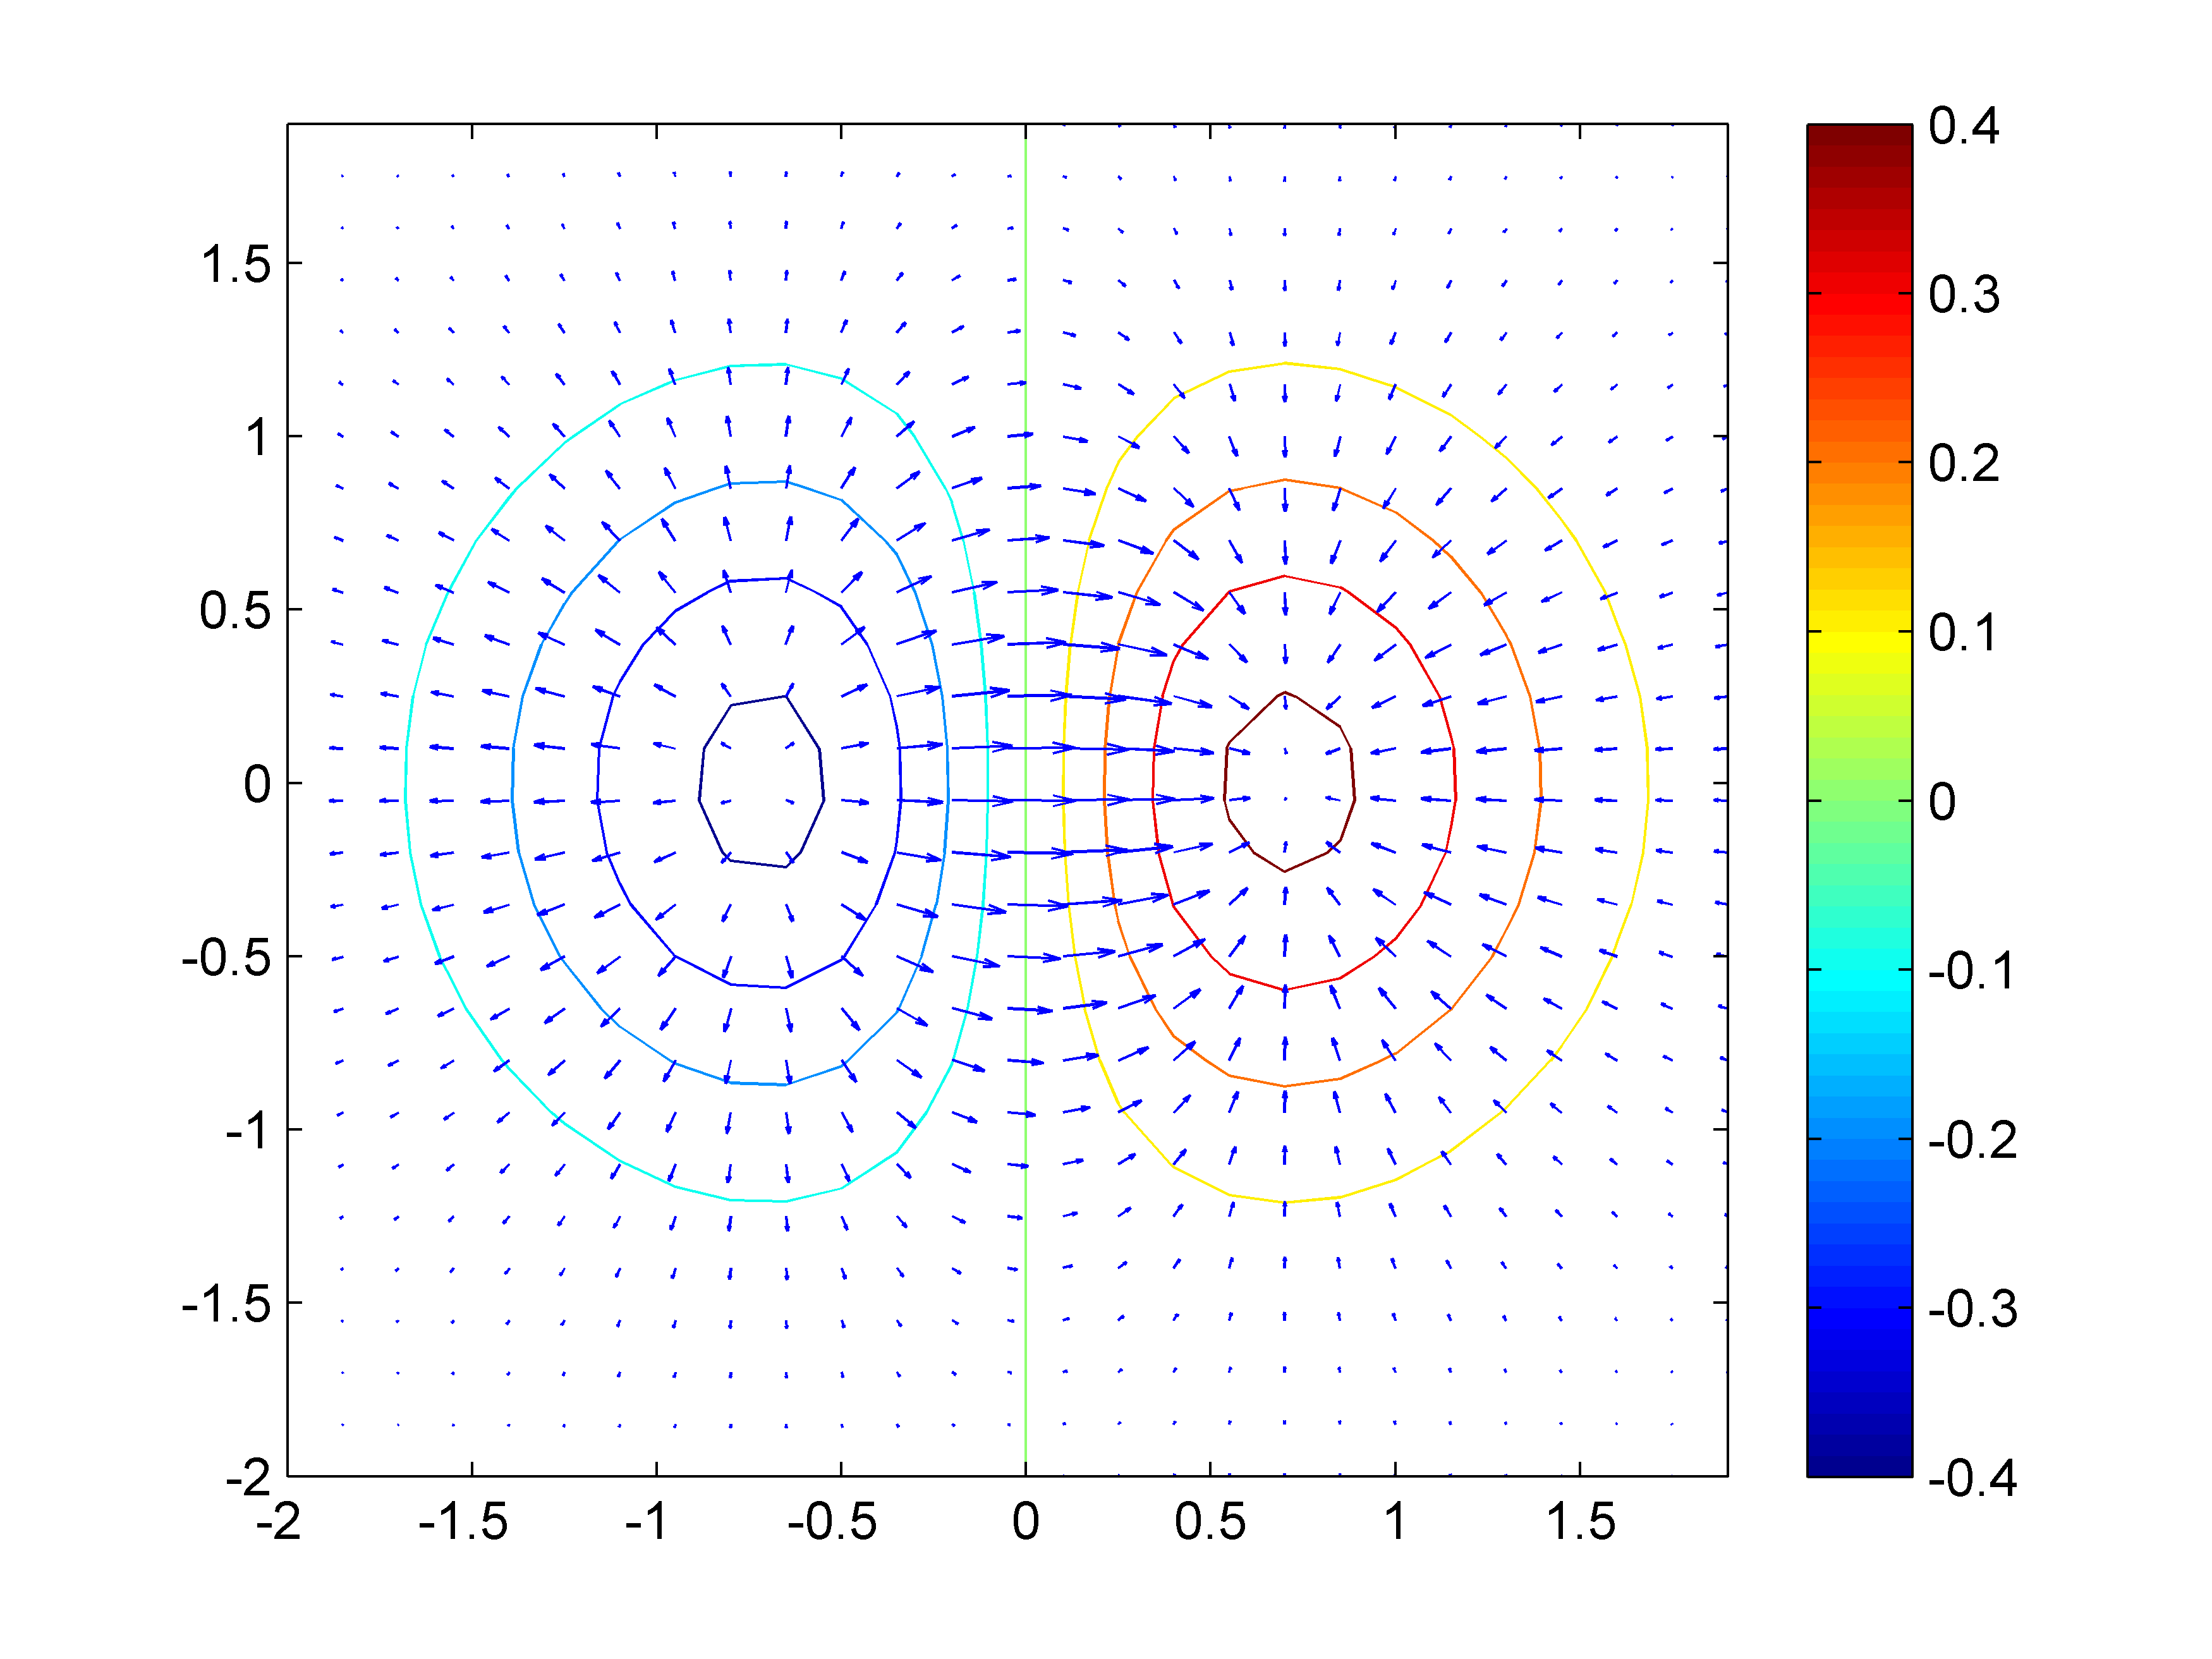
\includegraphics[width=400pt]{./Imagenes/cvector1.png}

Otro ejemplo podemos verlo con los campos vectoriales gradientes. Para ellos conviene utilizar la orden $[px,py]=gradient(f,hx,hy)$, que calcula una aproximación por diferencias al gradiente de f, utilizando $hx$, $hy$ como los desplazamientos en las direcciones de abscisas y ordenadas respectivamente, según las formulas:
\begin{center}
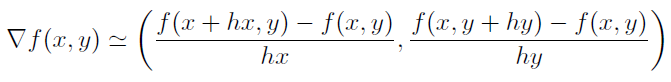
\includegraphics[width=300pt]{./Imagenes/grad.png}
\end{center}

Vamos a ver otro ejemplo. Para representar un campo vectorial, primero definimos las funciones componentes del campo, luego las restricciones para las variables que definen F, construir las matrices X e Y, finalmente con \textbf{quiver} dibujar el campo.

\begin{lstlisting}[language=Matlab]
>> u=inline('0*x+1','x','y'); 
>> v=inline('x+y.^2','x','y'); 
>> x=linspace(-2,3,11); 
>> y=linspace(-1,2,11); 
>> [X,Y]=meshgrid(x,y); 
>> U=u(X,Y);V=v(X,Y); 
>> quiver(X,Y,U,V) 
>> axis image 
\end{lstlisting}

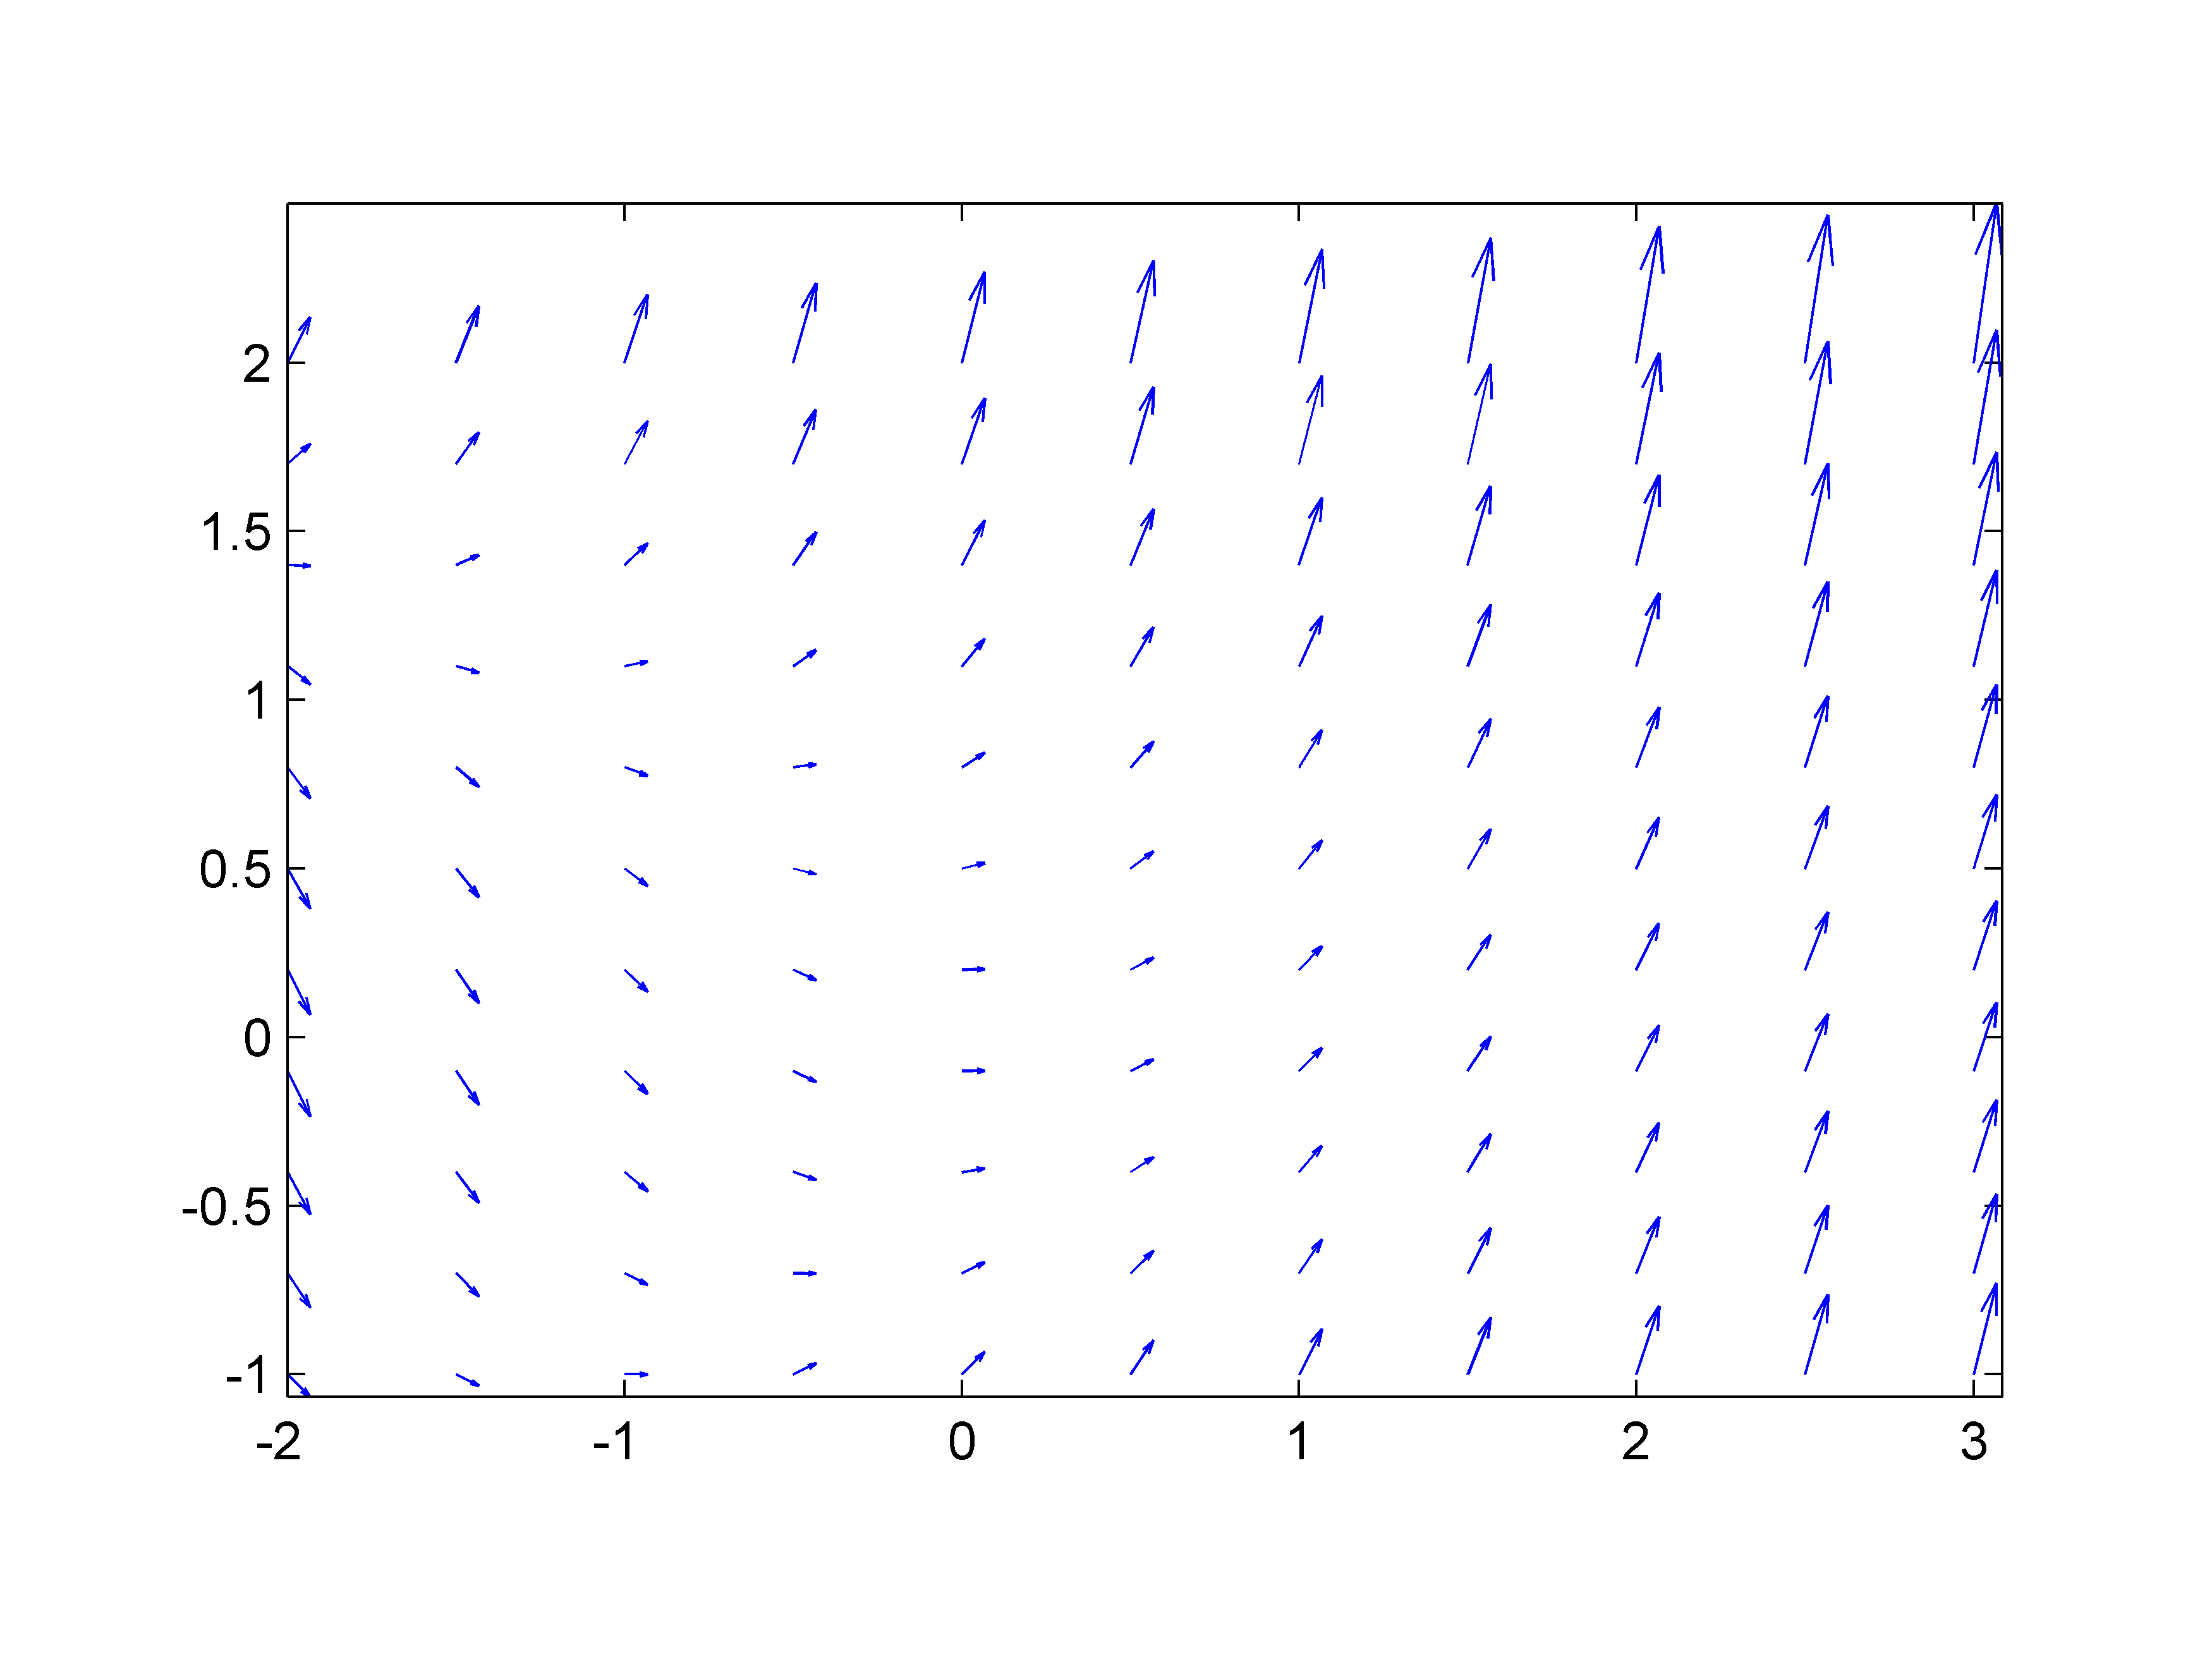
\includegraphics[width=400pt]{./Imagenes/vectorial1.png}
\chapter{Gráficos en 3D}

Con \textbf{MATLAB} Se pueden realizar curvas en el espacio y superficies 3D. Un ejemplo de curvas en el espacio son las curvas de nivel, las cuales en realidad son representaciones bi-dimensionales que tras su posterior interpretación nos conducen al entorno espacial.

Algunos tipos de gráficos 3D que se pueden realizar con \textbf{MATLAB}:
\begin{center}
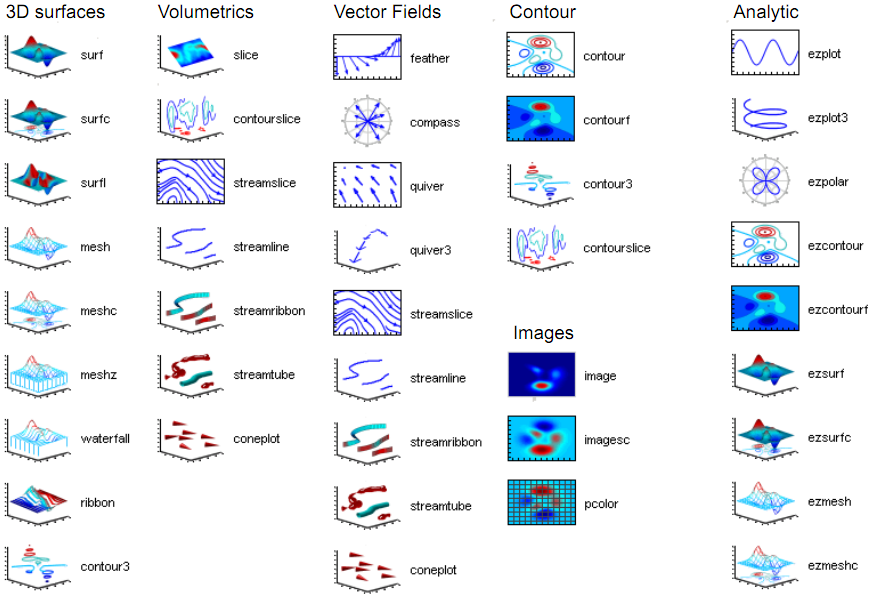
\includegraphics[width=450pt]{./Imagenes/graficos3d.png}
\end{center}

\section{Curvas en el espacio}

Existe una conexión muy estrecha entre las funciones vectoriales continuas de una variable con 
las curvas.

Una función vectorial \textbf{r} definida sobre un intervalo $I=[a,b]$, es una correspondencia entre los puntos de $I$ con los vectores del espacio, mediante $r(t)=(x(t),y(t),z(t)); t \in I$.

La función vectorial \textbf{r} es continua en \textbf{t=c} si y solo si sus funciones componentes \textbf{x,y,z} son continuas en \textbf{t=c}.

Dado un punto \textbf{P(x;y;z)} en el espacio, el vector $r(t)=x_{i}+y_{j}+z_{k}$ es el vector posición del punto \textbf{P}. A cada punto le corresponde un único vector posición y viceversa. 

\section{El comando plot3}

Este comando se utiliza para representar curvas en el espacio. Su funcionamiento y manejo es similar al del comando \textbf{plot}. La sintaxis del comando es:

\begin{lstlisting}[language=Matlab]
>> plot3(x,y,z,opciones)
\end{lstlisting}

En el campo opciones, se utilizan las mismas que vimos anteriormente para el comando \textbf{plot}.

El ejemplo que veremos a continuación corresponde a una curva alabeada $(x(t), y(t), z(t)), t \in [t_{0}, t_{f} ]$, con la orden $plot3(x,y,z)$:

\begin{lstlisting}[language=Matlab]
>> t=linspace(0,50,500);
>> x=t.*cos(t); y=t.*sin(t); z=t;
>> plot3(x,y,z)
>> xlabel('x(t)'); ylabel('y(t)'); zlabel('z(t)');
>> grid on; title('Curva con plot3');
\end{lstlisting}
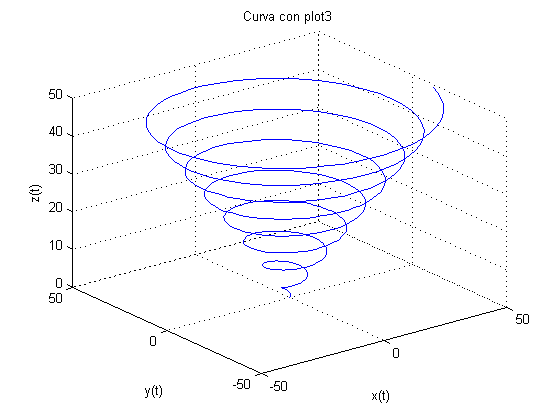
\includegraphics[width=300pt]{./Imagenes/3d1.png}


\section{El comando surf}

El comando \textbf{surf} se utiliza para representar superficies en el espacio. Esencialmente sirve para representar funciones de dos variables en el espacio. La sintaxis de este comando es:

\begin{lstlisting}[language=Matlab]
>> surf(x,y,z)
\end{lstlisting}

donde \textbf{X} e \textbf{Y} especifican una malla en el plano y \textbf{Z} la altura correspondiente. El color que se le da a cada punto esta asignado por defecto según la altura del eje Z.

Lo que debemos hacer ahora es construir una malla. Para esto utilizaremos el comando \textbf{meshgrid}. De esta forma podremos representar una superficie $ z = f(x,y) $ en un dominio rectangular, utilizando puntos de coordenadas $ x = (x_{1},\ldots, x_{n}) $ e $ y = (y_{1},\ldots, y_{n}) $. Con estos puntos podremos generar una malla donde los nuevos puntos sean $ x_{i},y_{j} $. En \textbf{MATLAB} simplemente tenemos que utilizar la orden

\begin{lstlisting}[language=Matlab]
>> [X,Y]=meshgrid(x,y)
\end{lstlisting}

que crea las matrices de \textit{m} x \textit{n} respectivas para X e Y.

\begin{center}
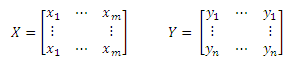
\includegraphics[width=150pt]{./Imagenes/matrices.png}
\end{center}


Es decir, las m filas de X son copias del vector x y las n columnas de Y son copias del vector y. La malla esta formada por los puntos $(X_{(i,j)},Y_{(i,j)})$. Por ejemplo,

\begin{lstlisting}[language=Matlab]
>> x=[0 0.33 0.67 1]; y=[-1 0 1];
>> [X,Y]=meshgrid(x,y)
X =
0 0.3300 0.6700 1.0000
0 0.3300 0.6700 1.0000
0 0.3300 0.6700 1.0000

Y =
-1 -1 -1 -1
 0  0  0  0
 1  1  1  1
\end{lstlisting}

Ahora para representar la superficie $z = f(x, y)$ utilizamos la orden \textbf{surf(X,Y,Z)} donde,

\begin{center}
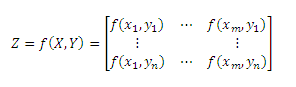
\includegraphics[width=150pt]{./Imagenes/matrices2.png}
\end{center}

A continuación vemos un ejemplo de superficie creada con el comando \textbf{surf}:

\begin{lstlisting}[language=Matlab]
>> x=linspace(-2,2,40);
>> y=linspace(-1,1,20);
>> [X,Y]=meshgrid(x,y);
>> Z=X.^2-Y.^2;
>> surf(X,Y,Z)
\end{lstlisting}
\begin{center}
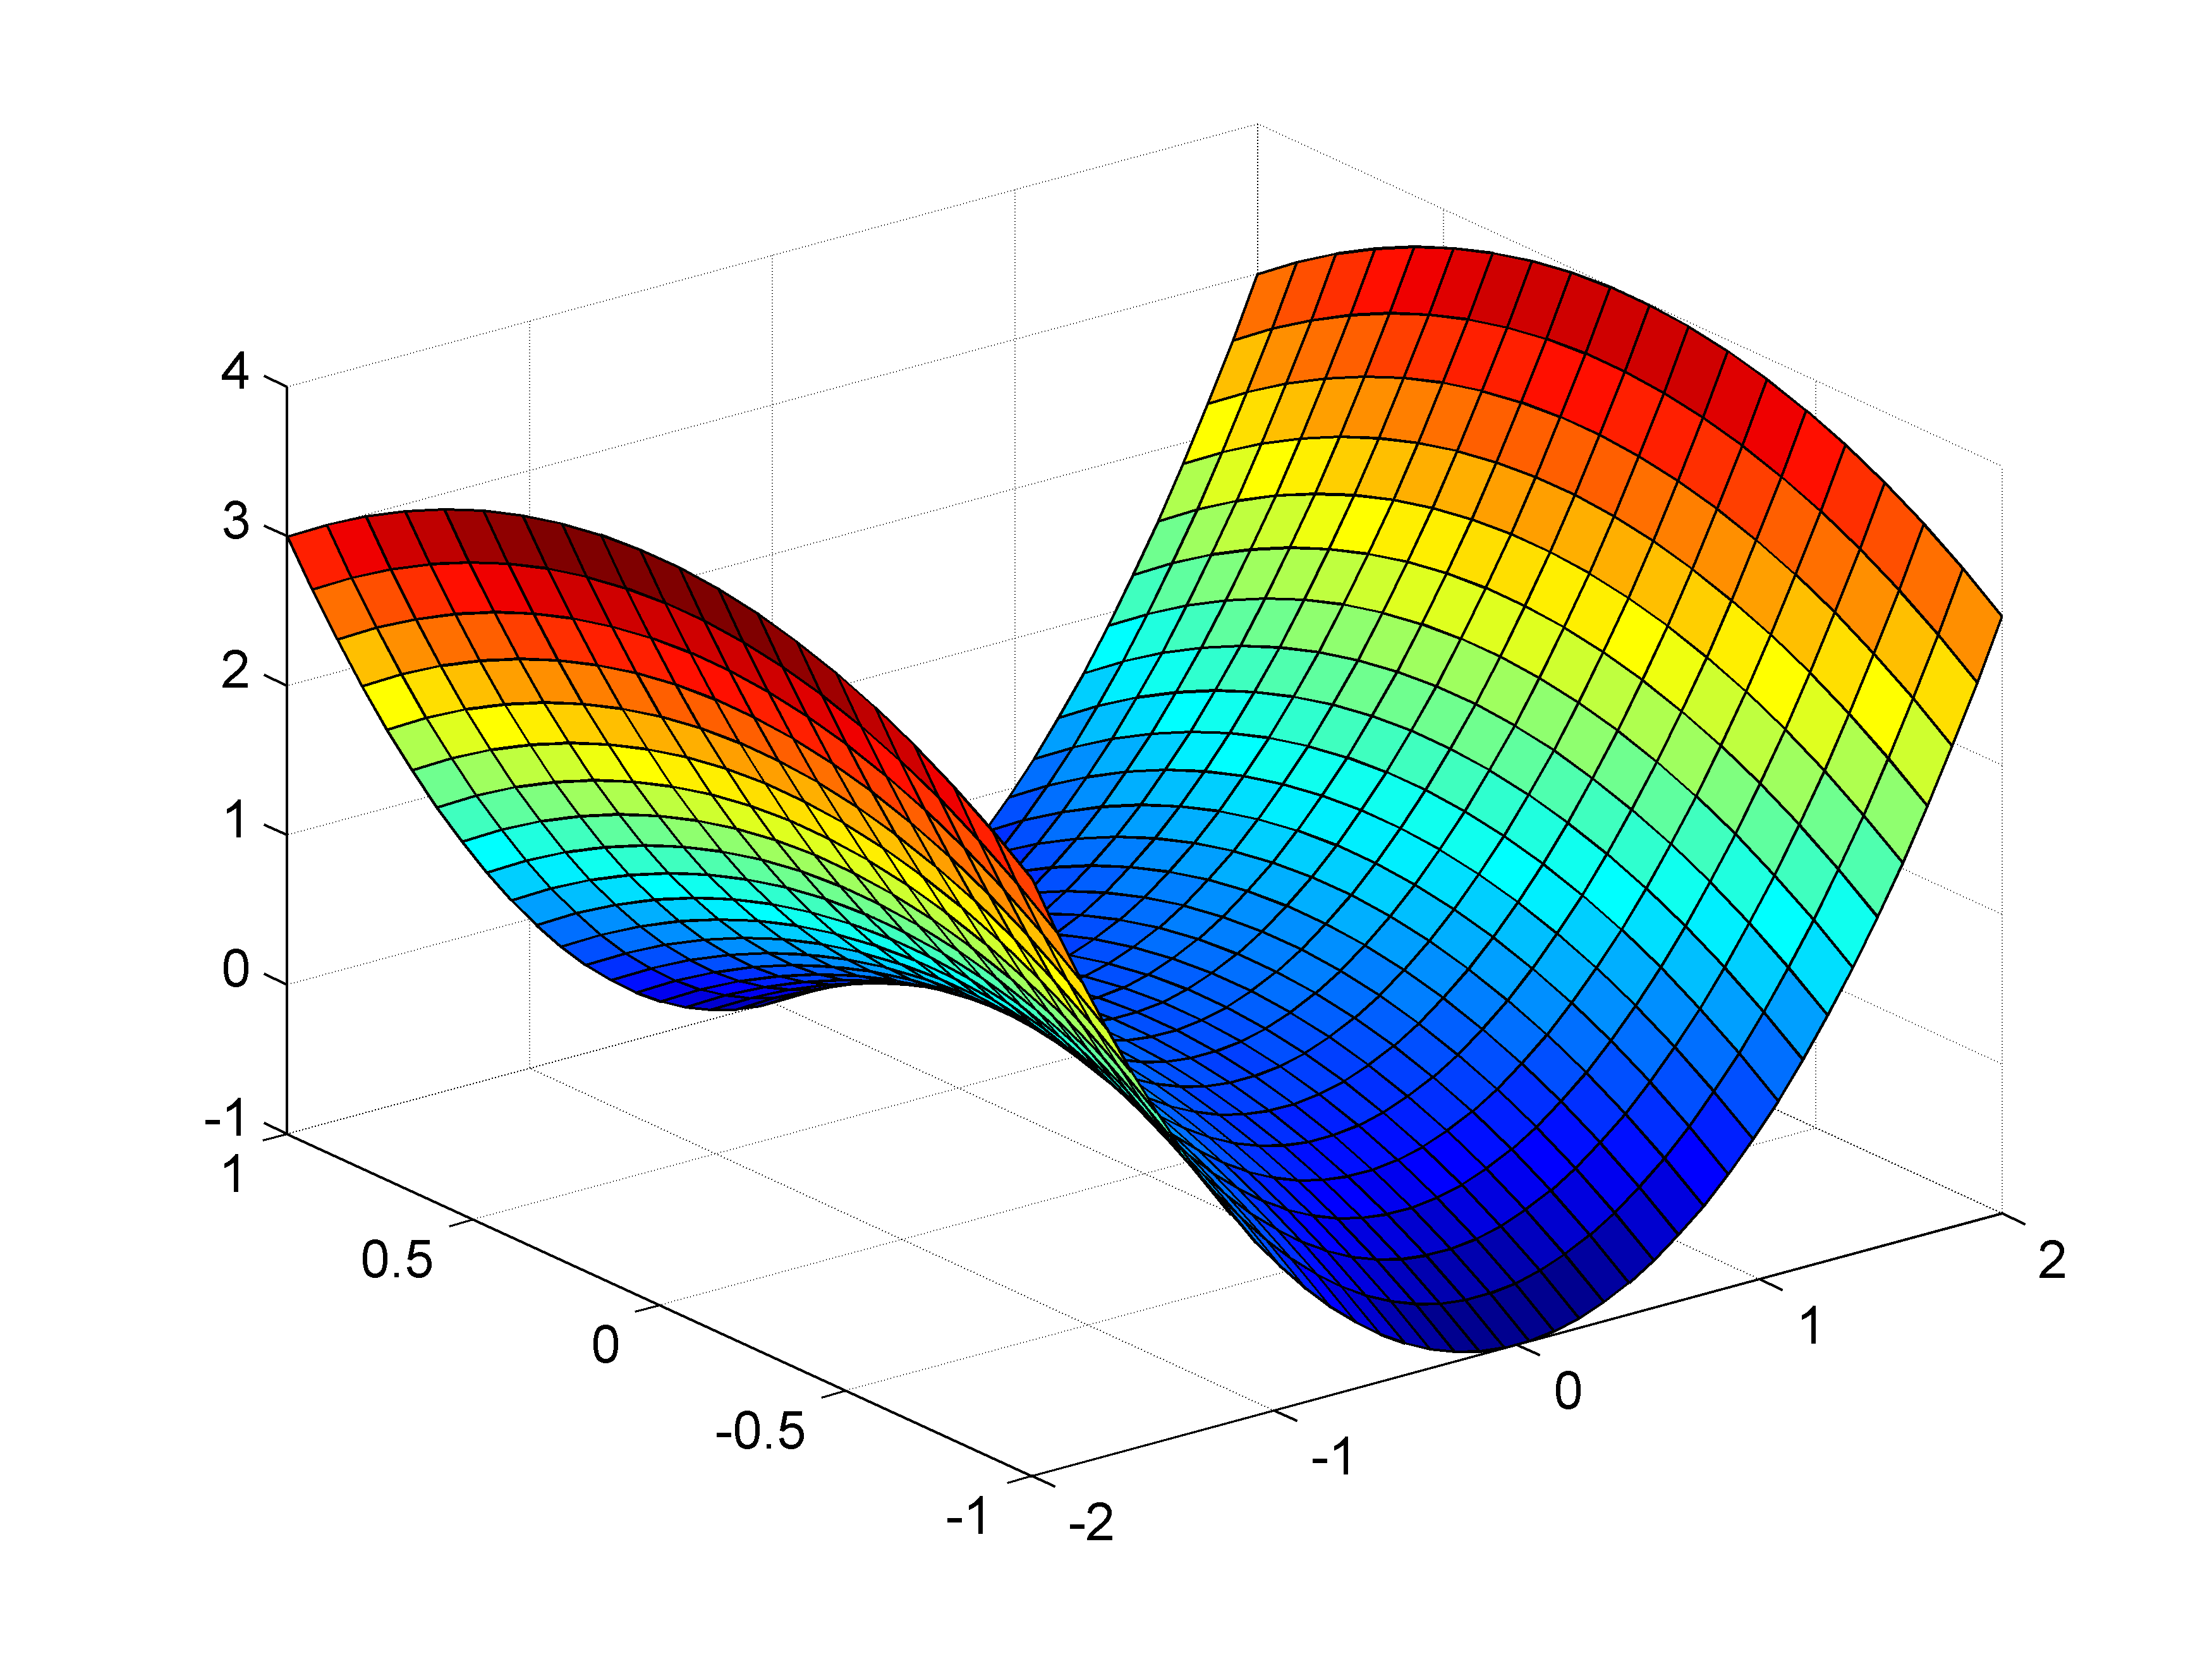
\includegraphics[width=300pt]{./Imagenes/surface1.png}
\end{center}

Se puede también dibujar una superficie y asignarle a esta un color según los valores de un cuarto vector.

\begin{lstlisting}[language=Matlab]
>> x=linspace(-3,3,60);
>> y=linspace(-3,3,60);
>> [X,Y]=meshgrid(x,y);
>> Z=X.^2-Y.^2;
>> T=cos(sqrt(X.^2+Y.^2+Z.^2));
>> surf(X,Y,Z,T), colorbar
\end{lstlisting}
\begin{center}
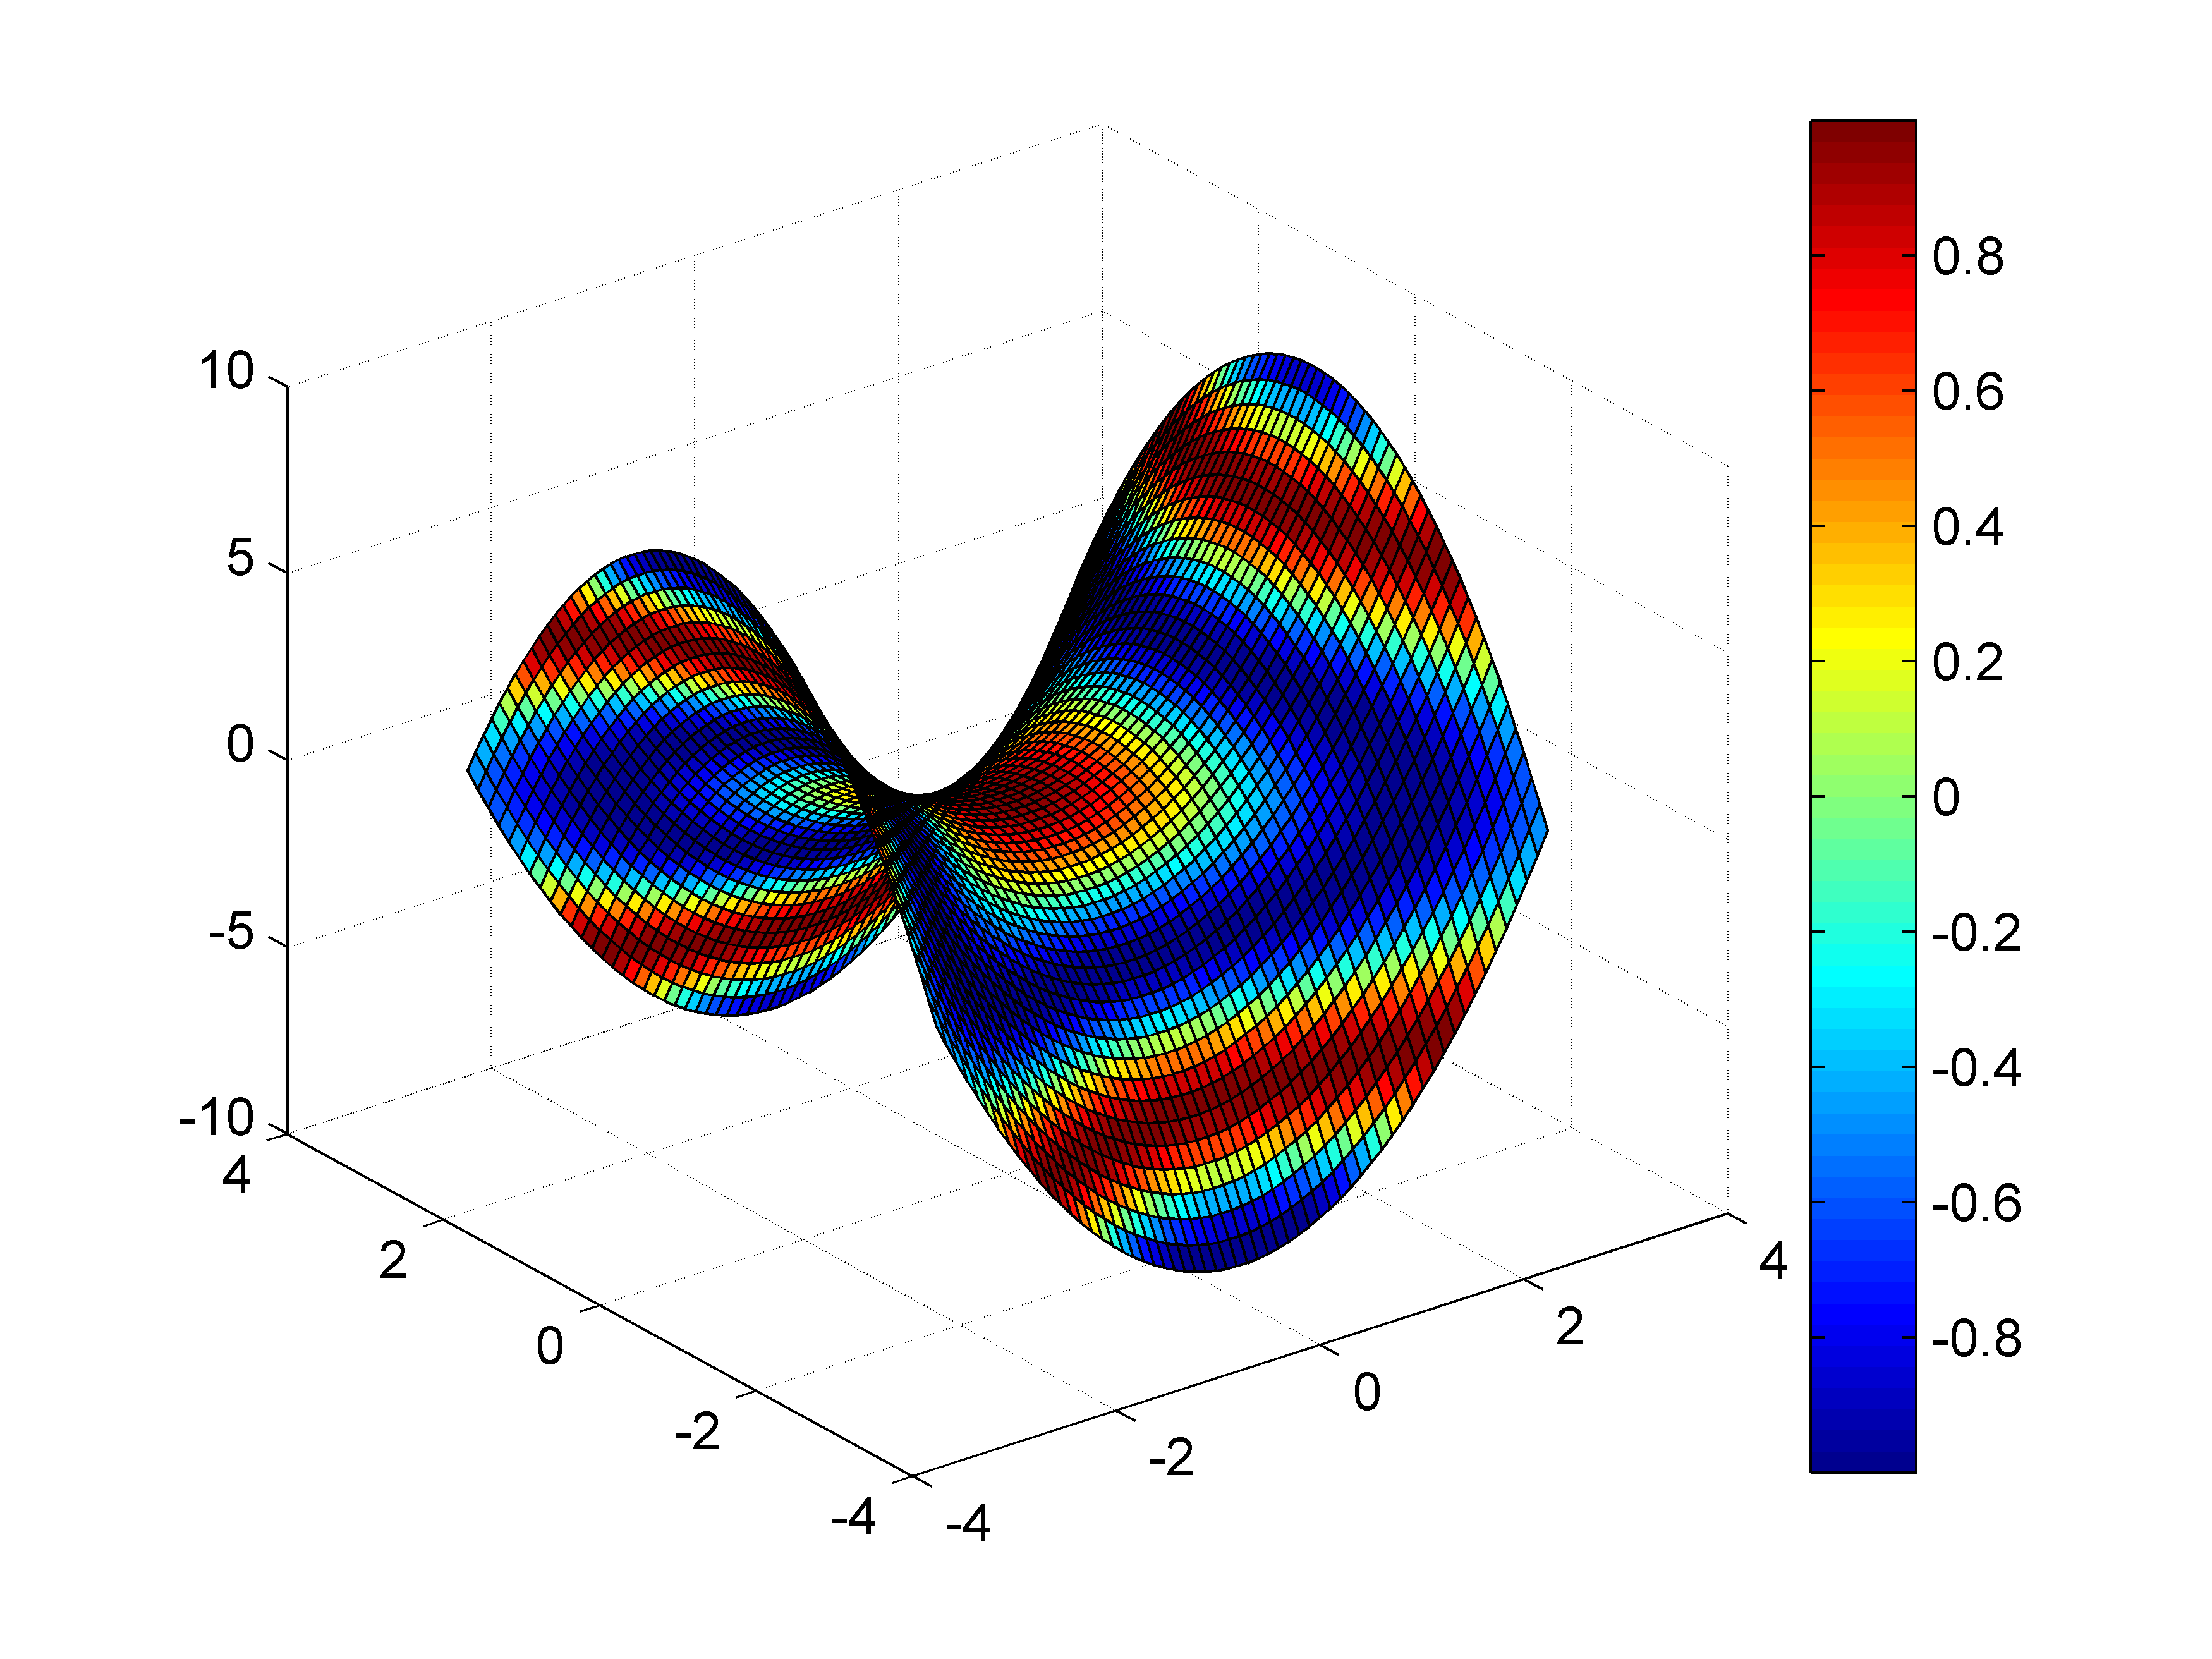
\includegraphics[width=300pt]{./Imagenes/surface2.png}
\end{center}

La orden $surf$ dibuja las superficies con colores sólidos. Se han introducido en la generación de las gráficas algunas especificaciones como:
\begin{lstlisting}[language=Matlab]
>> colormap(C) % Tabla de color usada para los graficos.
>> colorbar % Dibuja una barra de colores
>> shading flat % Quita la red del dibujo
>> shading interp % Varia el color en cada segmento
>> shading faceted % Defecto
\end{lstlisting}

A continuación se muestran algunos ejemplos de las gamas de colores que podemos usar junto al comando $colormap()$:
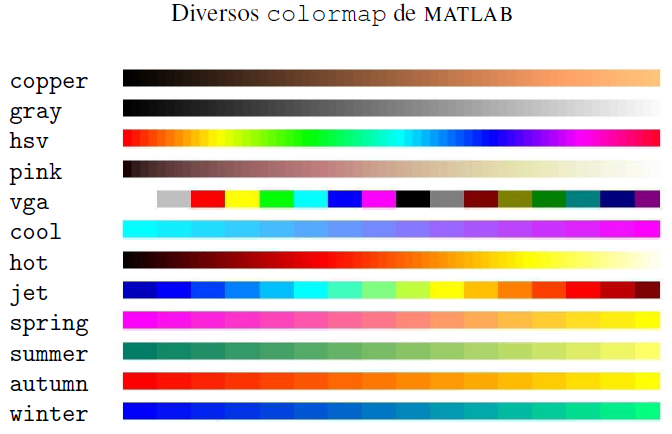
\includegraphics[width=300pt]{./Imagenes/3d4.png}

Ejemplo del uso del comando $surf$ con varias gráficas en una misma ventana:
\begin{lstlisting}[language=Matlab]
>> Z=membrane;
>> subplot(221), surf(Z)
>> subplot(222), surfc(Z)
>> subplot(223), surfc(Z), colorbar
>> subplot(224), surfc(Z), shading flat, colorbar
\end{lstlisting}

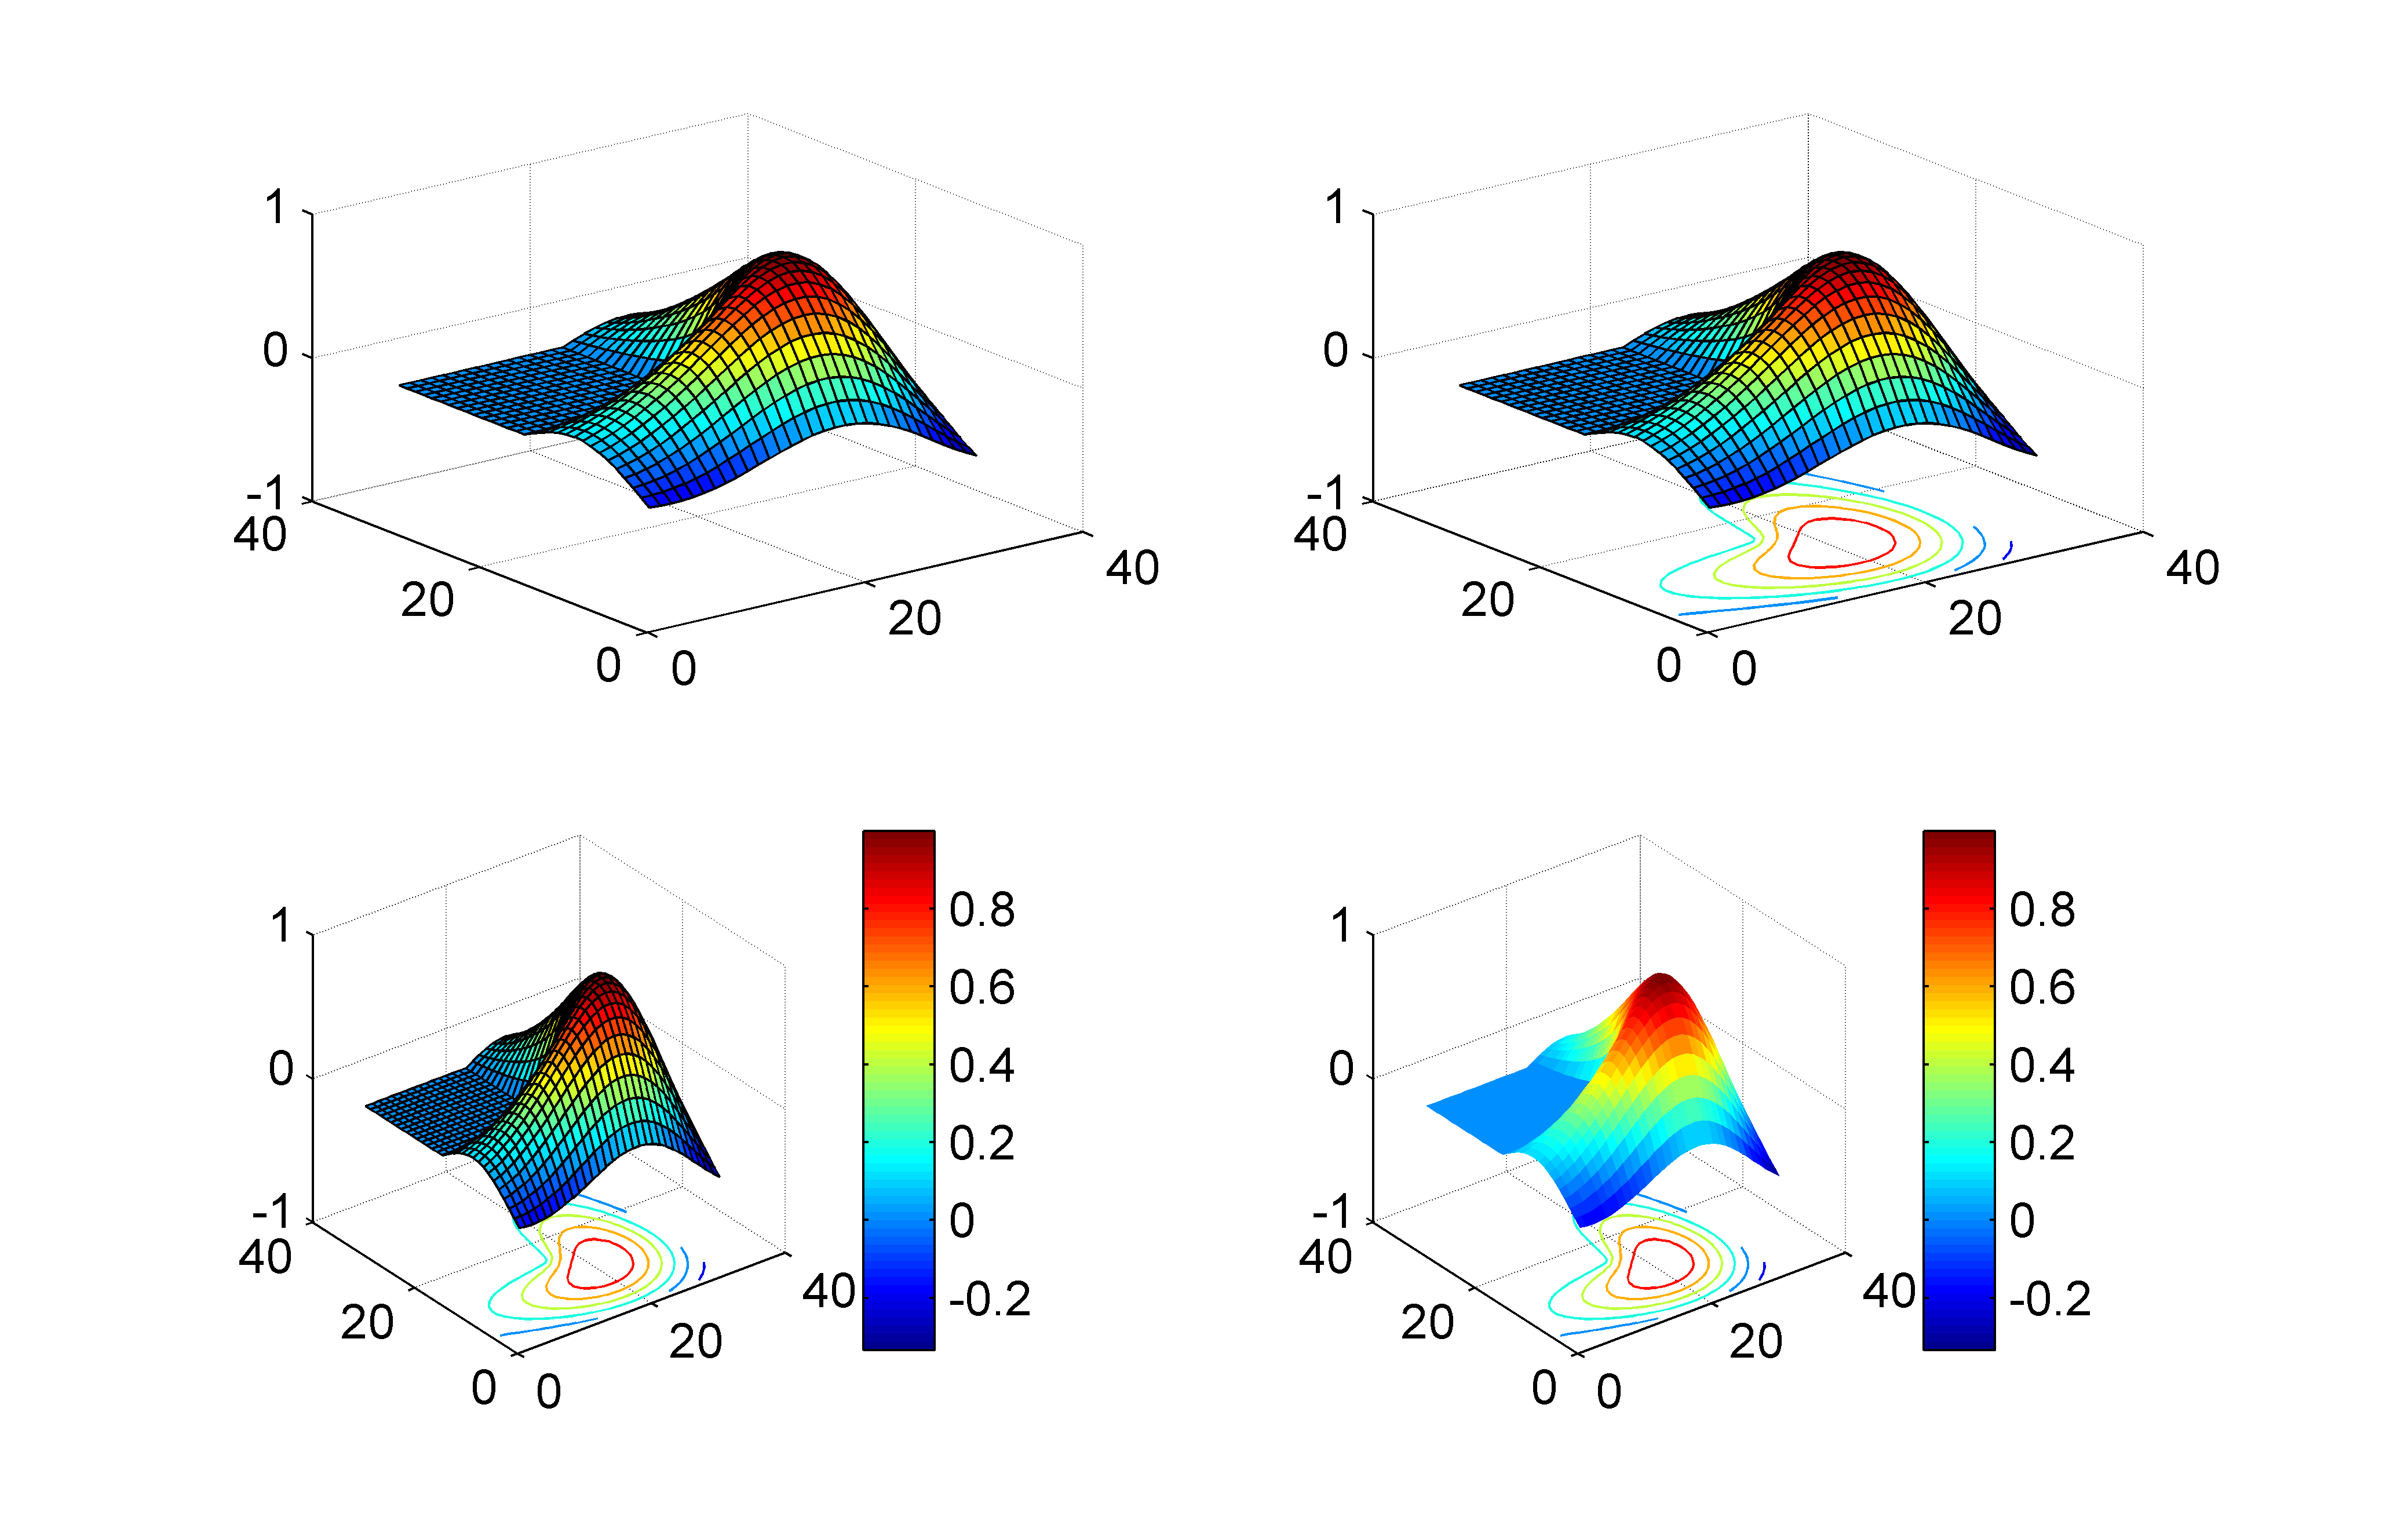
\includegraphics[width=400pt]{./Imagenes/3d5.png}

\section{Comandos de entorno 3D}

Hay 5 comandos importantes que describiremos a continuación. Sirven para manejar el entorno 3D, desde el color hasta el aspecto de la imagen.

\begin{itemize}
\item \textbf{colorbar}: despliega una barra de colores que informa sobre la correspondencia entre el valor numérico y el color utilizado. Por defecto aparece verticalmente a la derecha del dibujo aunque puede moverse posteriormente.
\item \textbf{colormap}: especifica que colores se van a utilizar en el dibujo. Existe un conjunto de formatos predefinidos listados a continuación. Para cambiar el formato de colores basta con utilizar el comando \textbf{colormap('opción')}:
\begin{itemize}
\item \textbf{autumn}
\item \textbf{gray}
\item \textbf{prism}
\item \textbf{bone}
\item \textbf{hot}
\item \textbf{spring}
\item \textbf{colorcube}
\item \textbf{hsv}
\item \textbf{summer}
\item \textbf{cool}
\item \textbf{jet}
\item \textbf{white}
\item \textbf{copper}
\item \textbf{lines}
\item \textbf{winter}
\item \textbf{flag}
\item \textbf{pink}
\item \textbf{default}
\end{itemize}

\item \textbf{daspect}: controla la relación entre los ejes del gráfico. Por ejemplo, mediante la siguiente instrucción se establece que los ejes X, Y y Z sean iguales. 
\begin{lstlisting}[language=Matlab]
>> daspect([1 1 1])
\end{lstlisting}

\item \textbf{pbaspect}: similar al comando anterior, pero este esta relacionado con la caja que enmarca al gráfico.
\item \textbf{view}: especifica desde donde se ve el gráfico. El comando tiene dos parámetros:
\begin{lstlisting}[language=Matlab]
>> view(az,el)
\end{lstlisting}
El primer parámetro es azimuth (angulo de rotación horizontal) y el segundo parámetro es el angulo de elevación vertical. Estos dos parámetros se deben especificar en grados. Por defecto, \textbf{MATLAB} le asigna a los gráficos 3D los valores de az=-37.5 y el=30.
\end{itemize}

\section{Comandos contour y mesh}
Para dibujar una superficie $z = f(x,y)$ en un dominio $D = [x_{0}, x_{f}] * [y_{0}, y_{f}]$, primero hay que definir una malla con el comando $meshgrid$ y luego evaluar $z = f(x, y)$ en dicha malla.
\begin{lstlisting}[language=Matlab]
>> [X,Y]=meshgrid( x0:xpaso:xf, y0:ypaso:yf);
>> Z=f(X,Y);
\end{lstlisting}

Las ordenes de dibujo 3D más usuales son:
\begin{lstlisting}[language=Matlab]
>> contour(X,Y,Z,num) - Genera las curvas de nivel
>> mesh(X,Y,Z) - Dibuja la  Z (ejes cartesianos)
>> meshc(Z) - mesh + contour (ejes matriciales)
>> meshc(X,Y,Z) - mesh + contour (ejes cartesianos)
>> surf(Z) - Dibujo solido (ejes matriciales)
>> surf(X,Y,Z) - Dibujo solido (ejes cartesianos)
\end{lstlisting}

Veamos un ejemplo de dibujo de curvas de nivel con la orden contour:
\begin{lstlisting}[language=Matlab]
>> [X,Y]=meshgrid( -4:0.1:4, -4:0.1:4);
>> Z= sin(X + Y.^2/10) + cos(X.^2-Y) + 0.5;
>> % Dibujo por defecto. (Ejes cartesianos)
>> subplot(221)
>> contour(X,Y,Z)
>> % Dibujar 5 curvas de nivel con relleno.
>> subplot(222)
>> contourf(X,Y,Z,5)
>> % Dibujar valores determinados de las curvas de
>> % nivel y etiquetarlos
>> subplot(223)
>> val = [-1 0 1. 2.];
>> [C,h] = contour(X,Y,Z,val);
>> clabel(C,h,val);
>> % Forma sencilla de dibujar curvas de nivel.
>> subplot(224)
>> ezcontour('sin(x+y^2/10)+cos(x^2-y)+.5',[-4,4,-4,4]);
\end{lstlisting}
\begin{center}
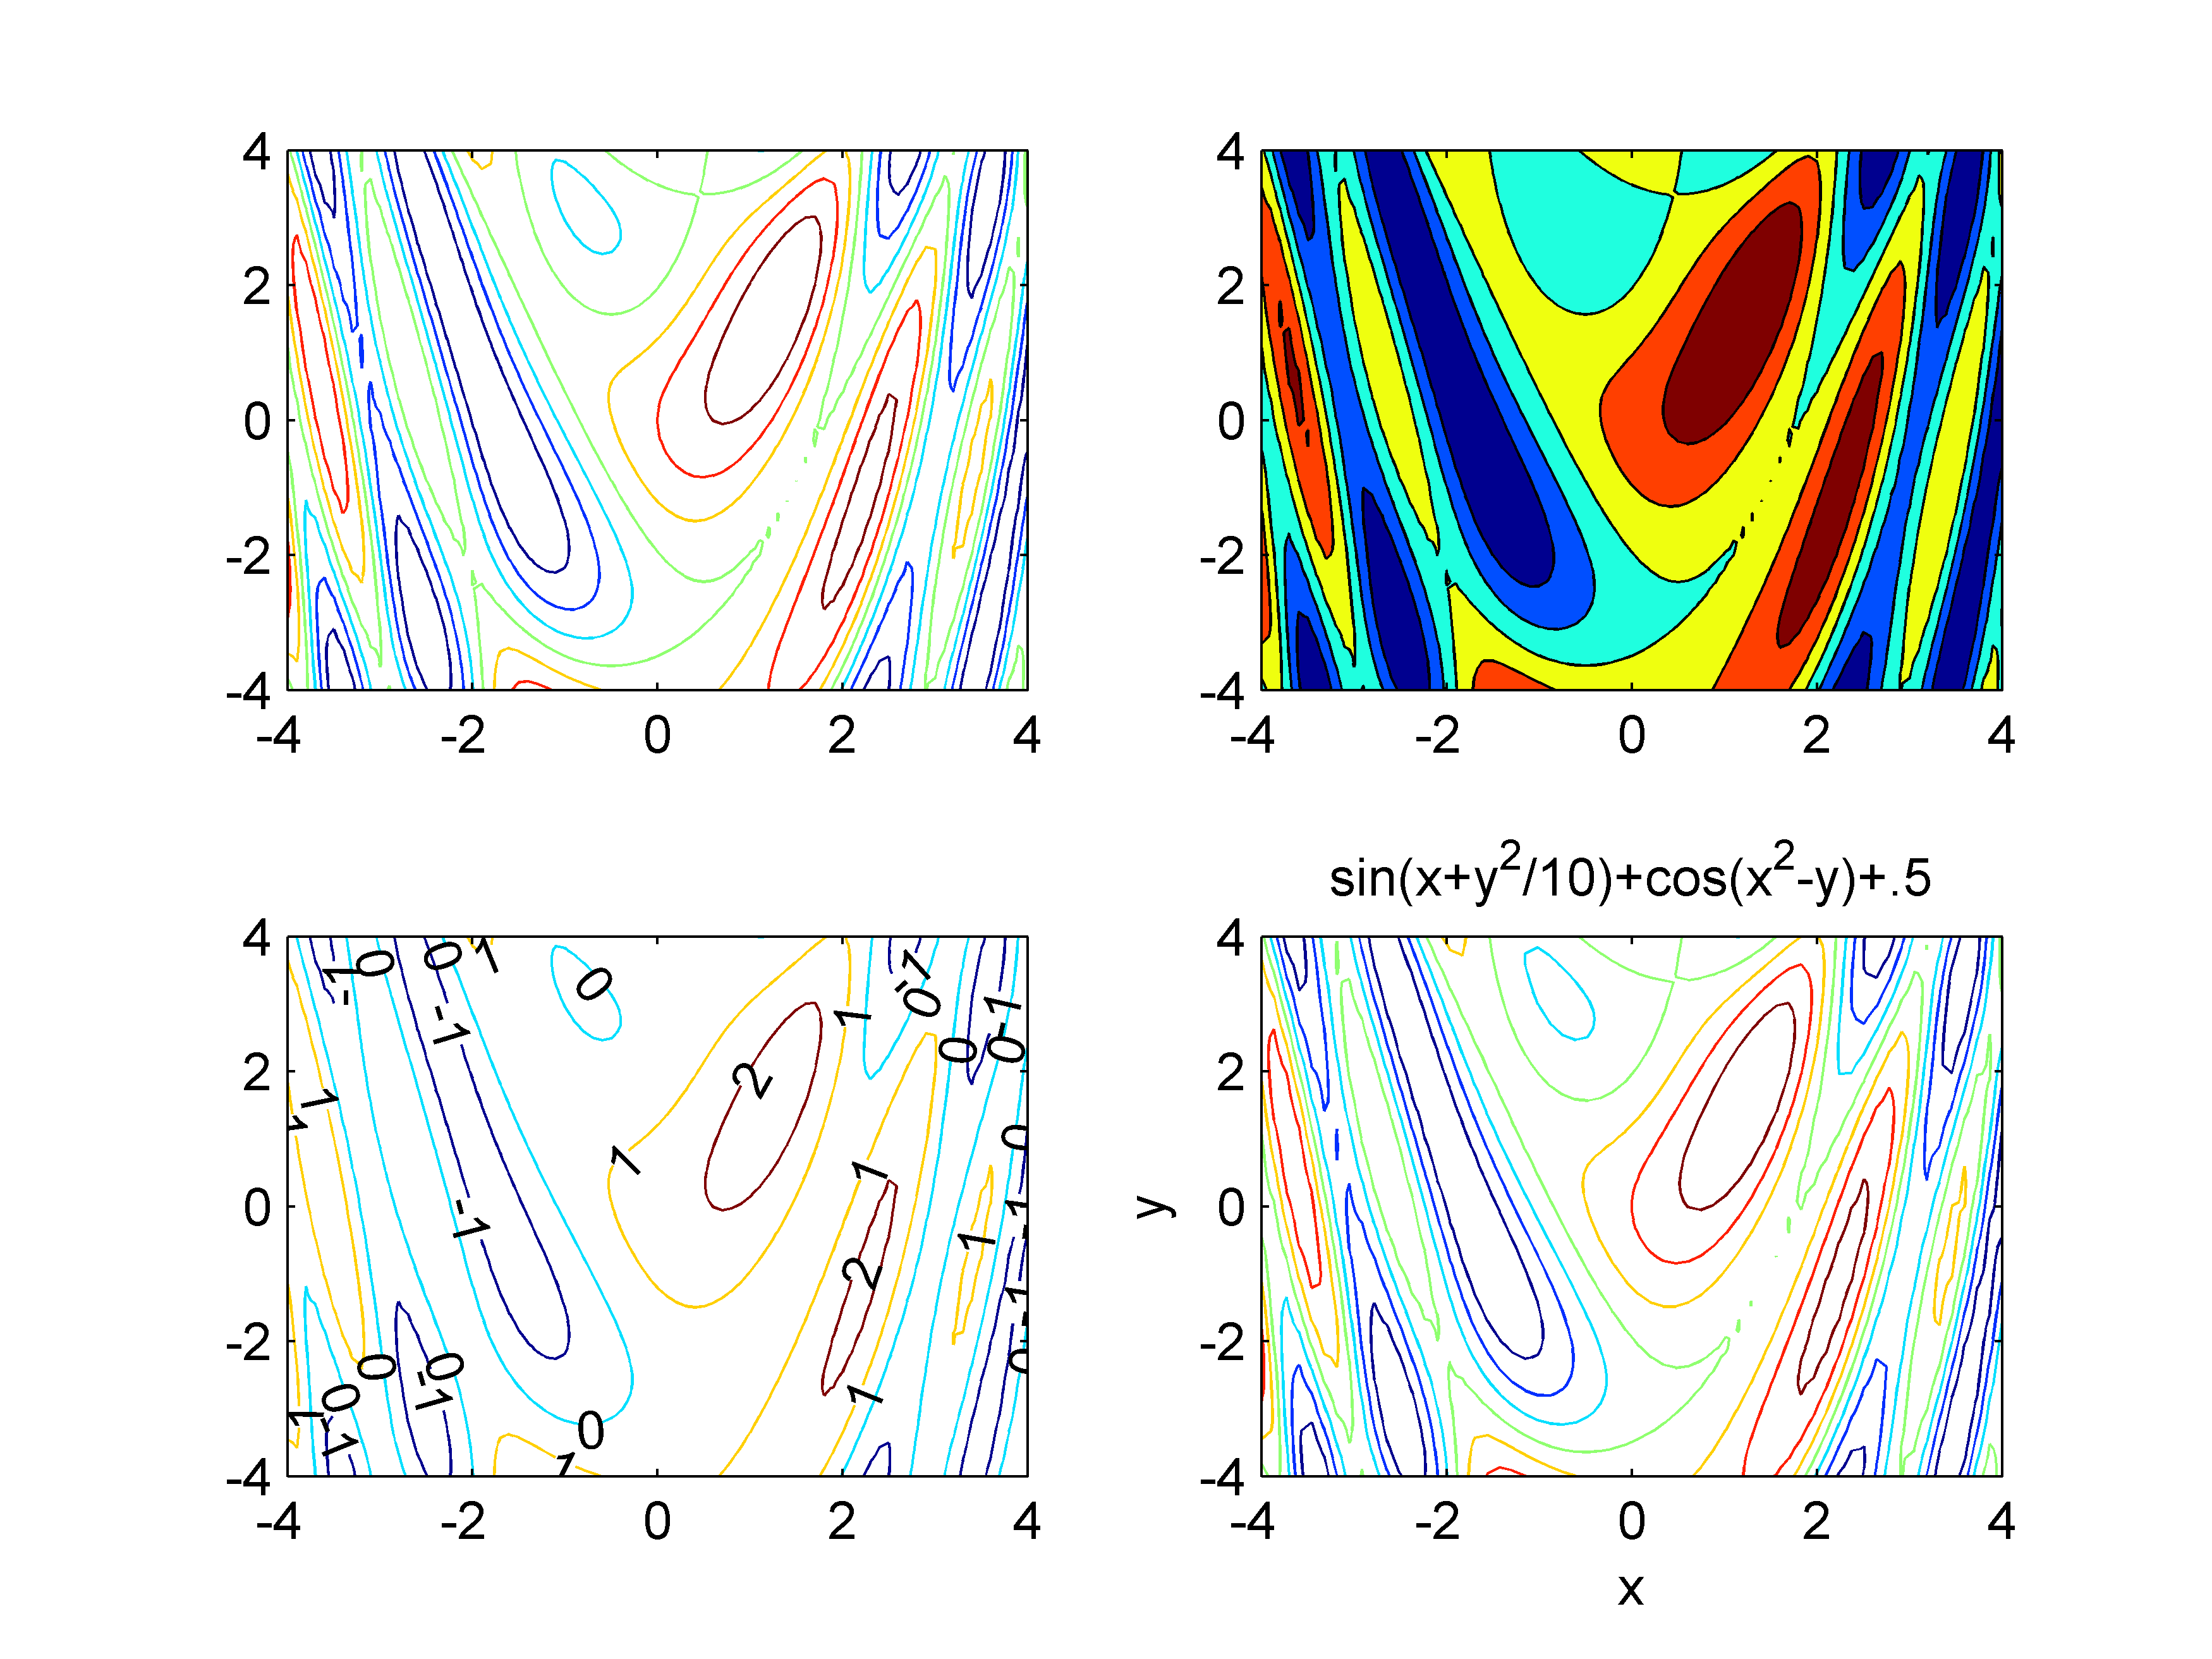
\includegraphics[width=300pt]{./Imagenes/3d2.png}
\end{center}

\subsection{Comando mesh}

La orden $mesh$ dibuja la superficie como si fuera una malla, veamos un ejemplo:
\begin{lstlisting}[language=Matlab]
>> [X,Y]=meshgrid( -4:0.5:4, -4:0.5:4);
>> Z= sin(X).*cos(Y);
>> subplot(221)
>> meshc(X,Y,Z)
>> xlabel('\bf x'); ylabel('\bf y'); zlabel('\bf z');
>> subplot(222)
>> mesh(X,Y,Z)
>> subplot(223)
>> mesh(X,Y,Z) % ejes cartesianos
>> axis([-6 6 -6 6 -4 4]);
>> subplot(224)
>> mesh(Z) % ejes matriciales
\end{lstlisting}
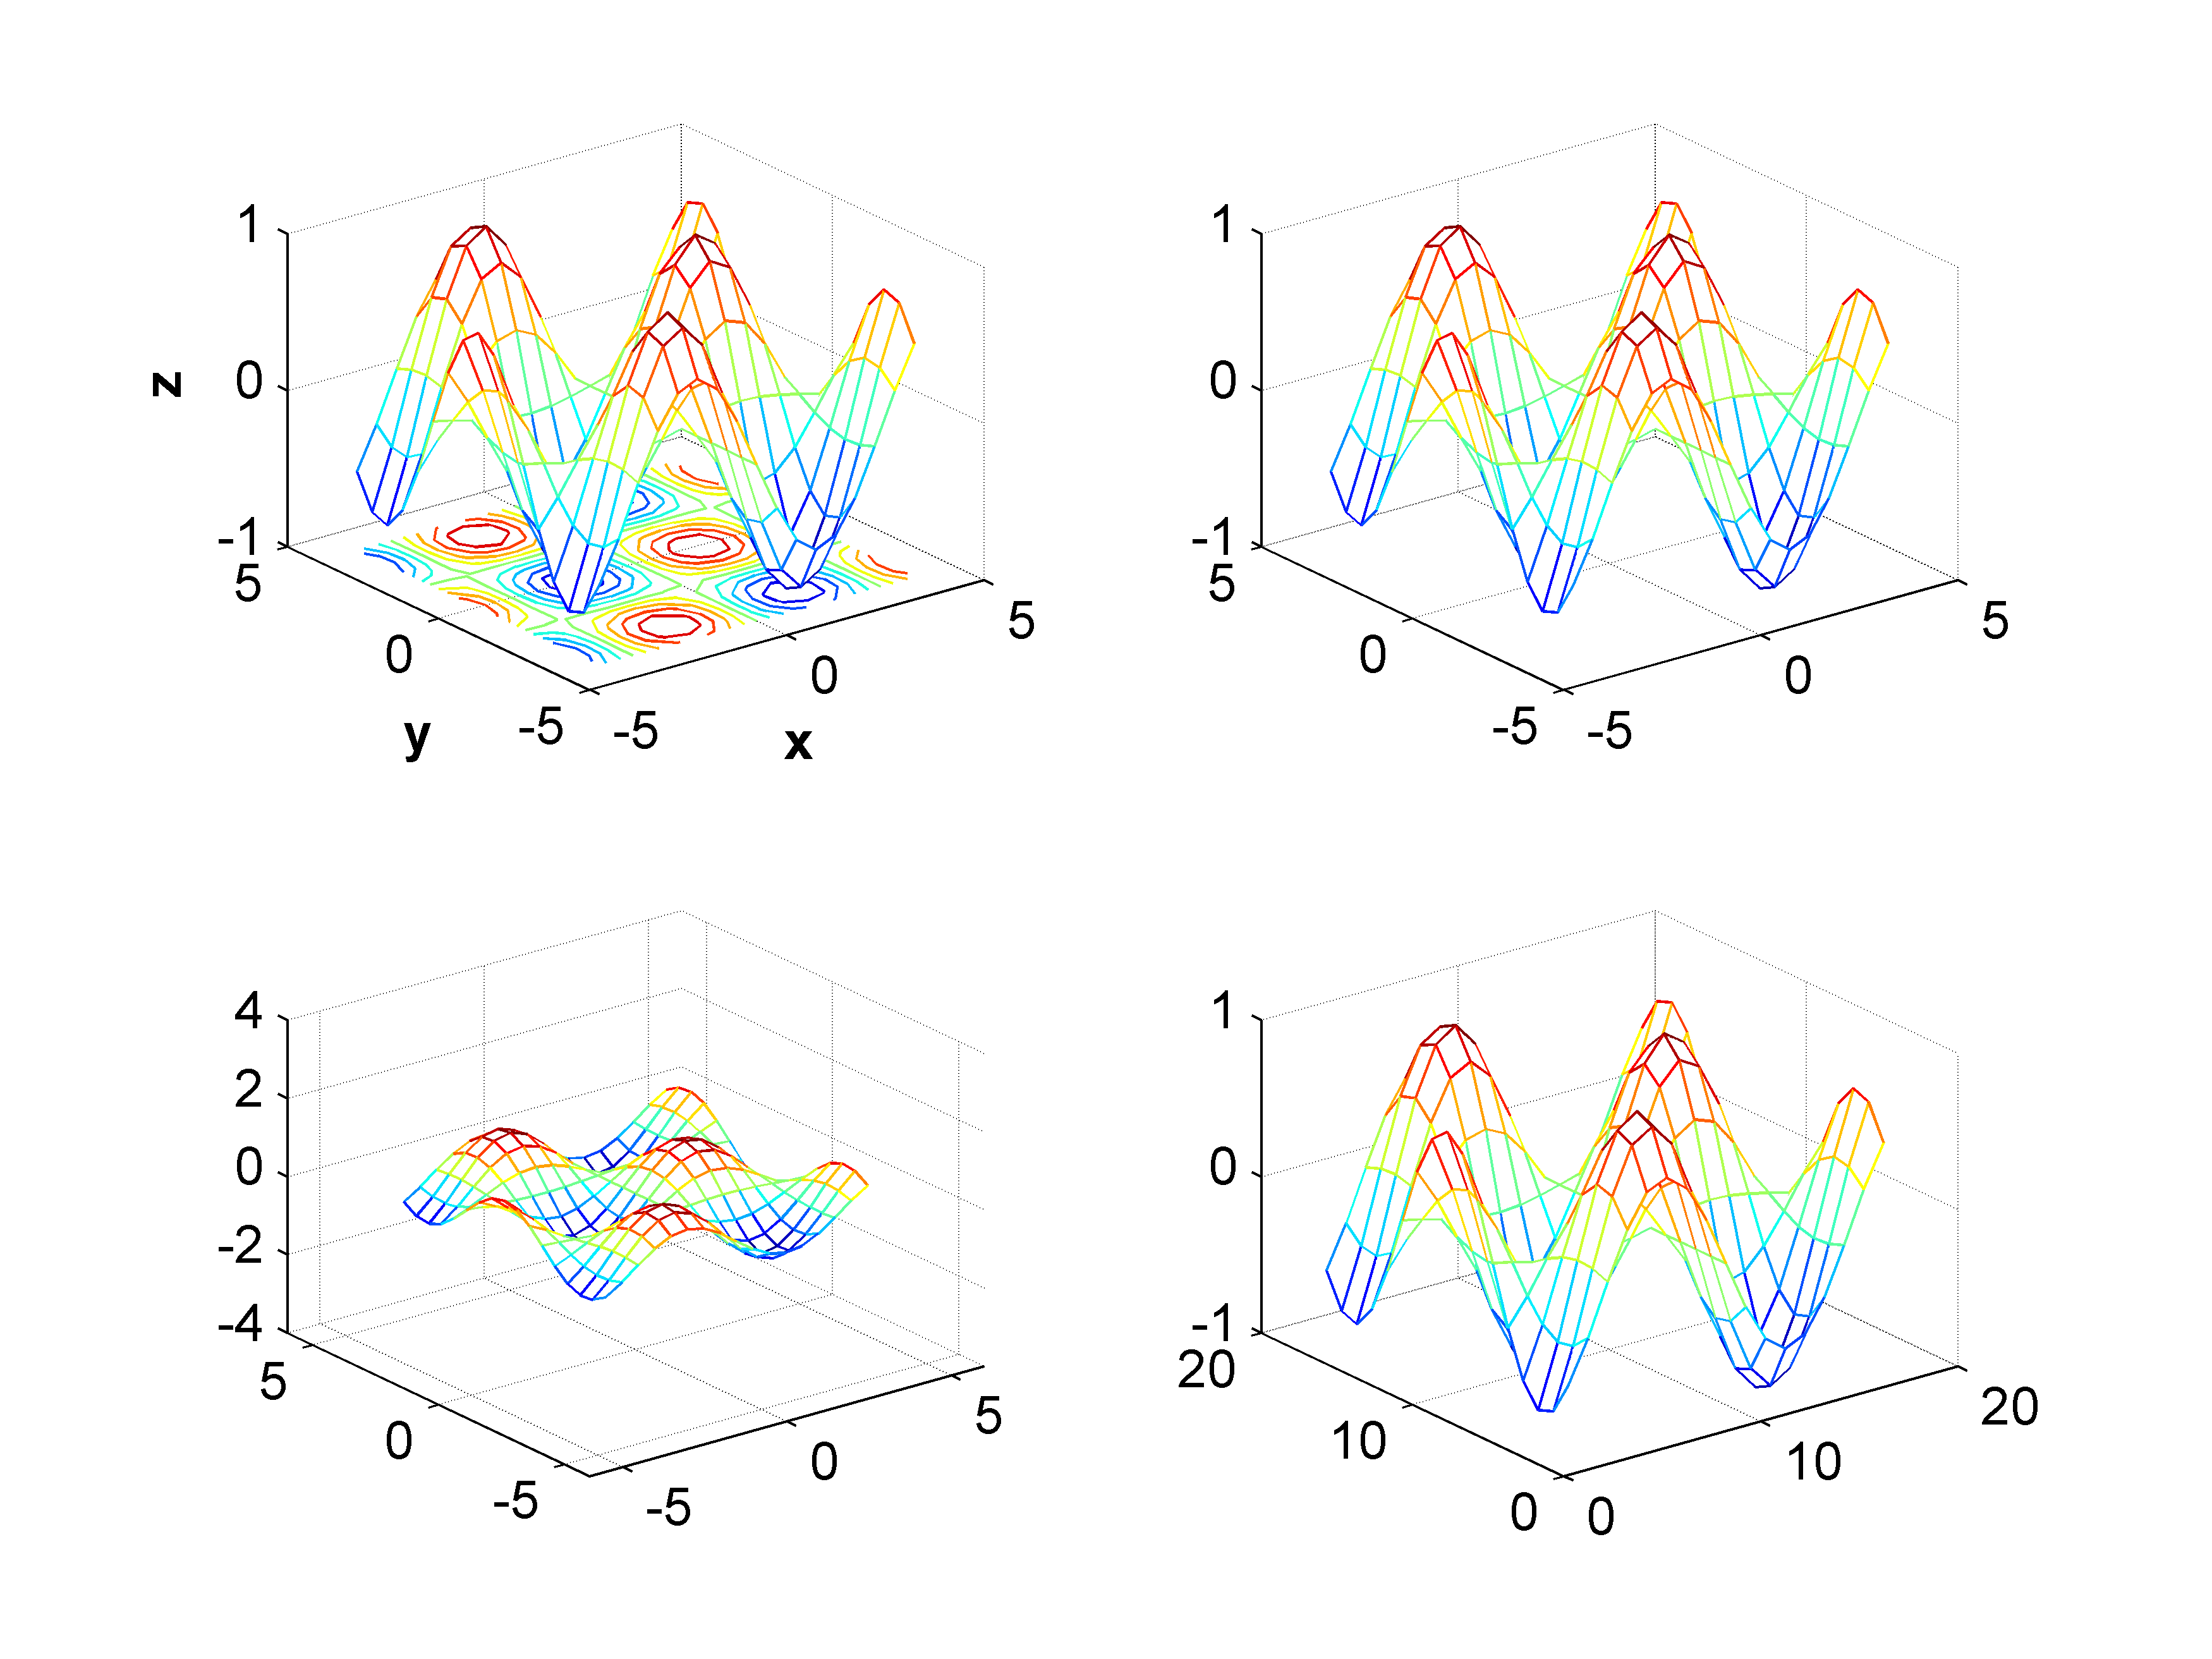
\includegraphics[width=300pt]{./Imagenes/3d3.png}


\section{Complementos}

La sentencia $surf$ puede utilizarse con cuatro parámetros (X,Y,Z,C), donde C representa la escala de color. \textbf{MATLAB} escala C para obtener los colores del actual colormap. Si solo hay tres parámetros, entonces $C=Z$, es decir el color es proporcional a la altura. Esto puede aprovecharse para representar una función $g(x, y, z)$ sobre la superficie definida por $(x, y, z)$.

\paragraph{Ejemplo 1}:
\begin{lstlisting}[language=Matlab]
>> [X,Y]=meshgrid(-3:0.05:3,-3:0.05:3);
>> Z=exp(-X.^2-Y.^2);
>> surf(X,Y,Z, X.^2+Y.^2+Z.^2), shading interp
>> colorbar
\end{lstlisting}
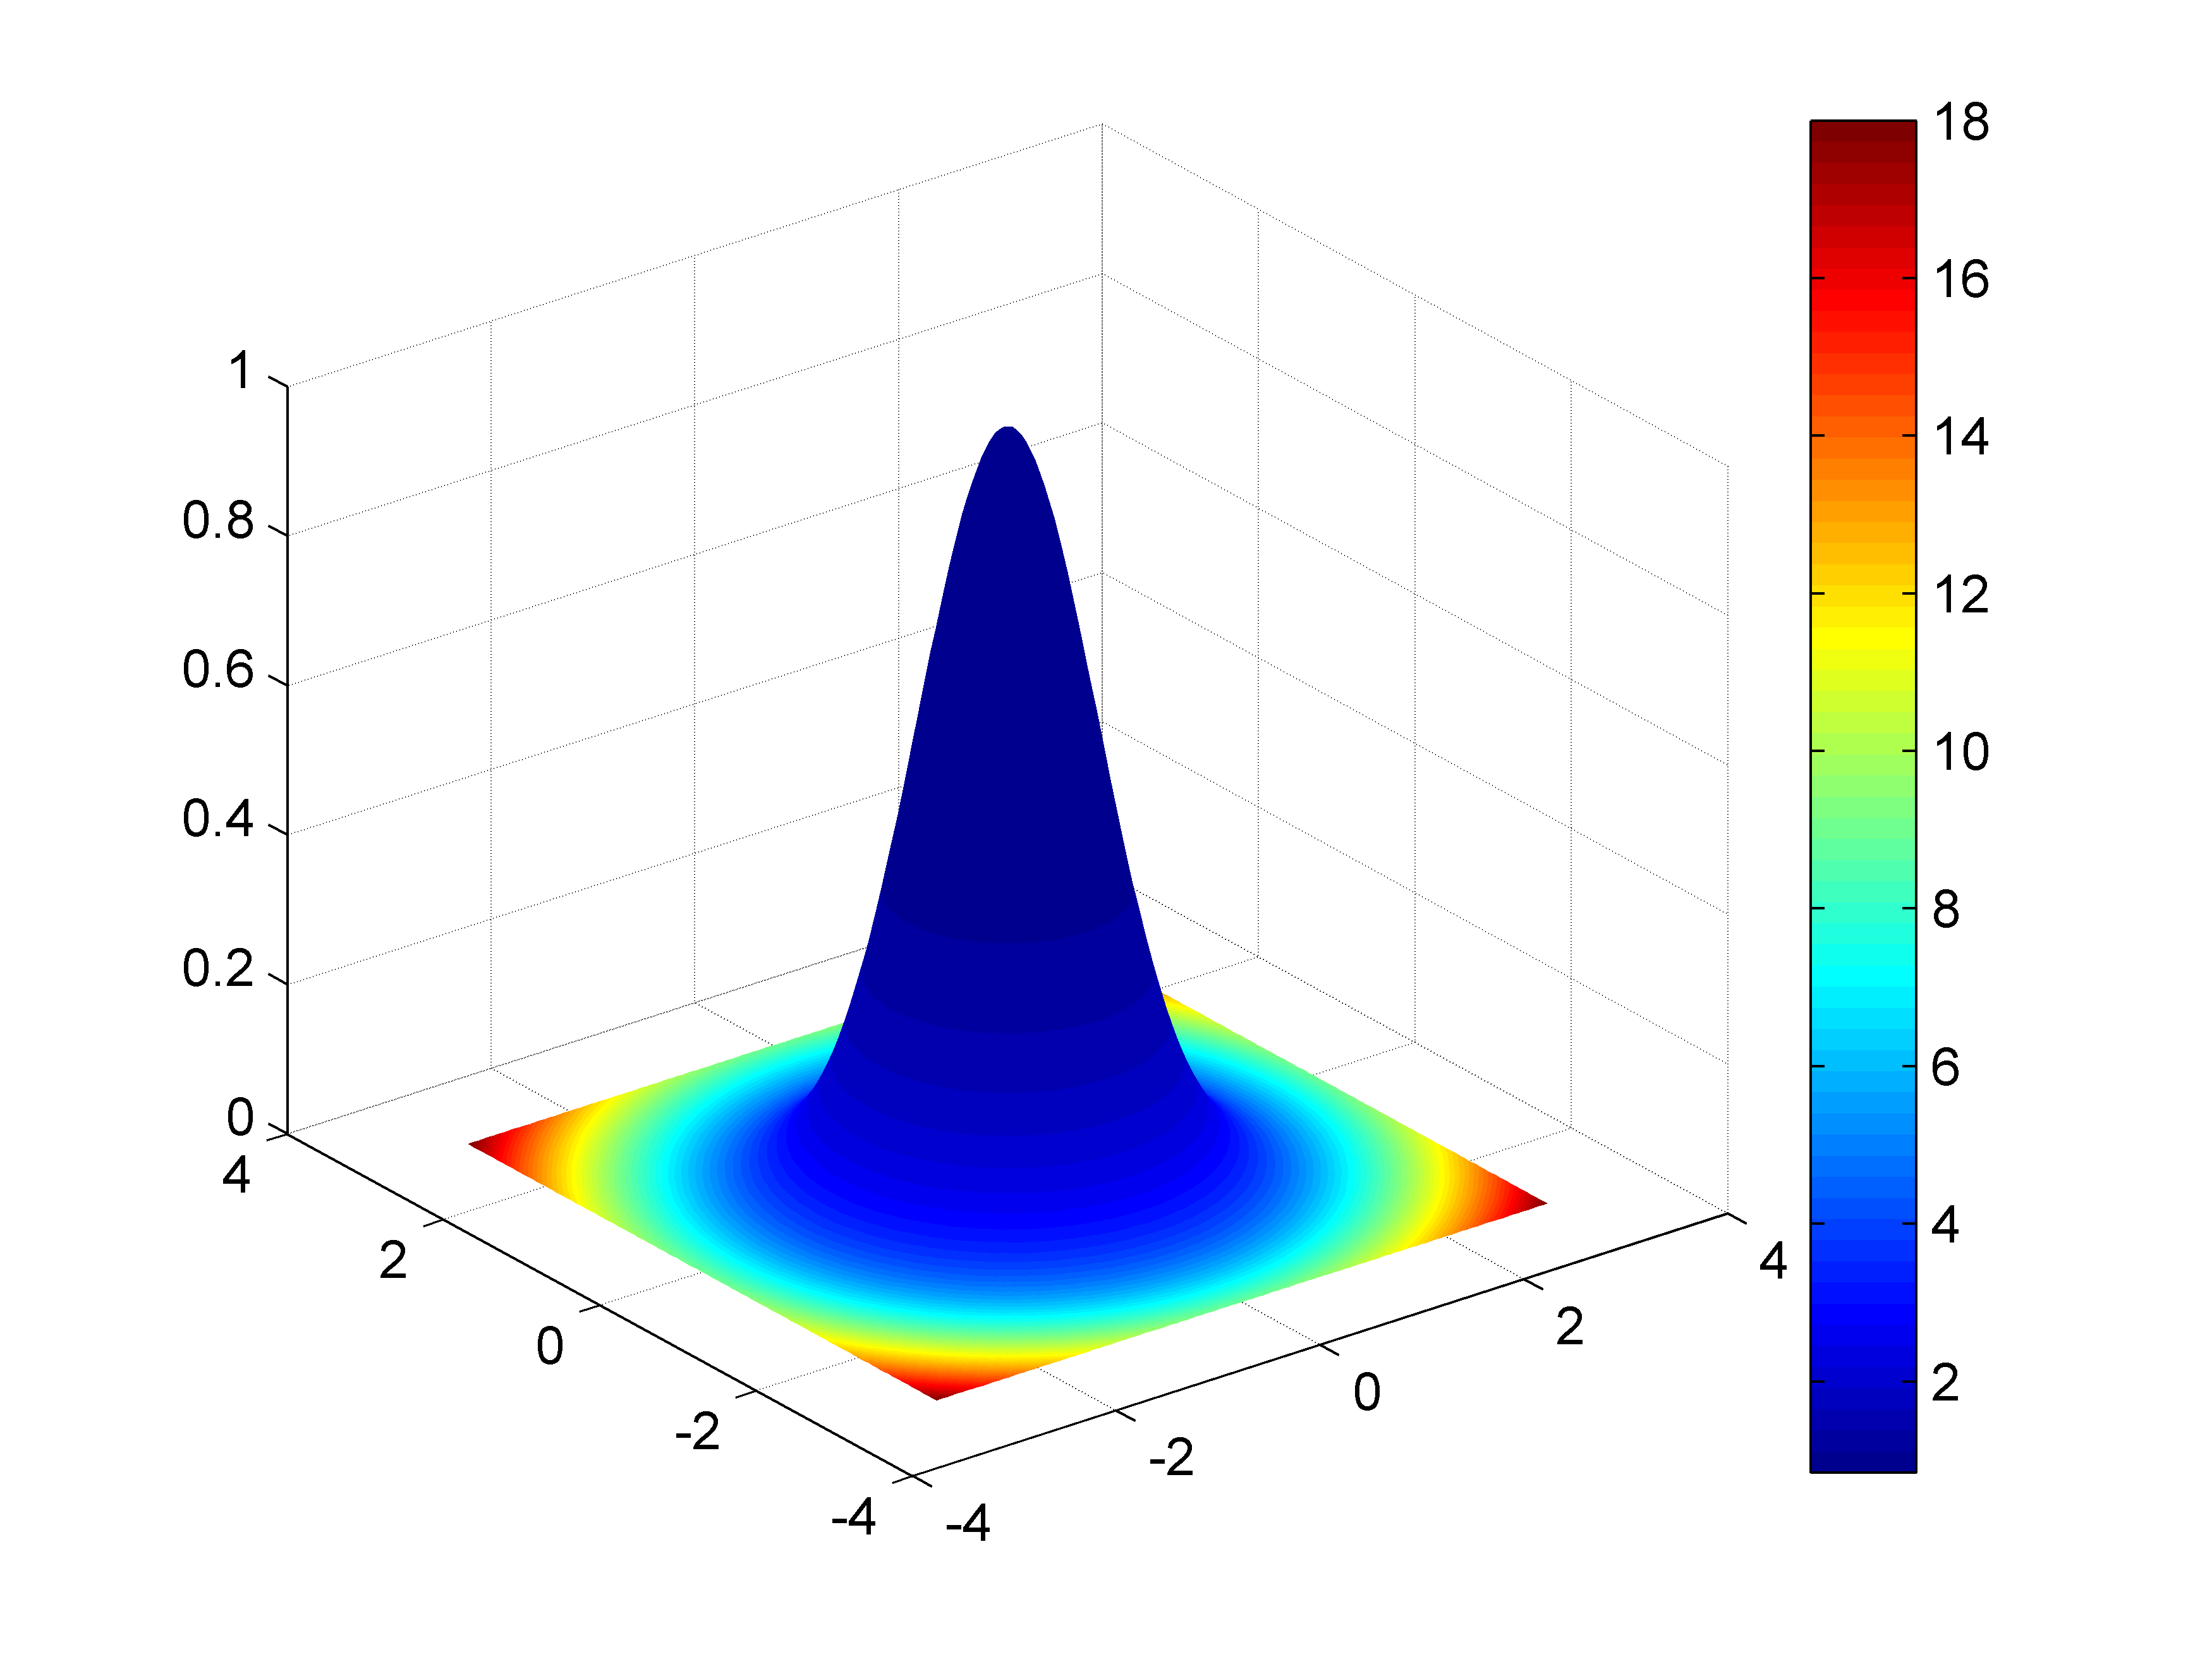
\includegraphics[width=300pt]{./Imagenes/3d6.png}

\paragraph{Ejemplo 2}:
\begin{lstlisting}[language=Matlab]
>> [X,Y]=meshgrid(-3:0.05:3,-3:0.05:3);
>> Z=cos(X).*cos(Y); Z(X.*Y > 2 & X.*Y<3)=NaN;
>> surf(X,Y,Z, X+Y+Z), shading interp
>> colormap('copper'); colorbar
\end{lstlisting}
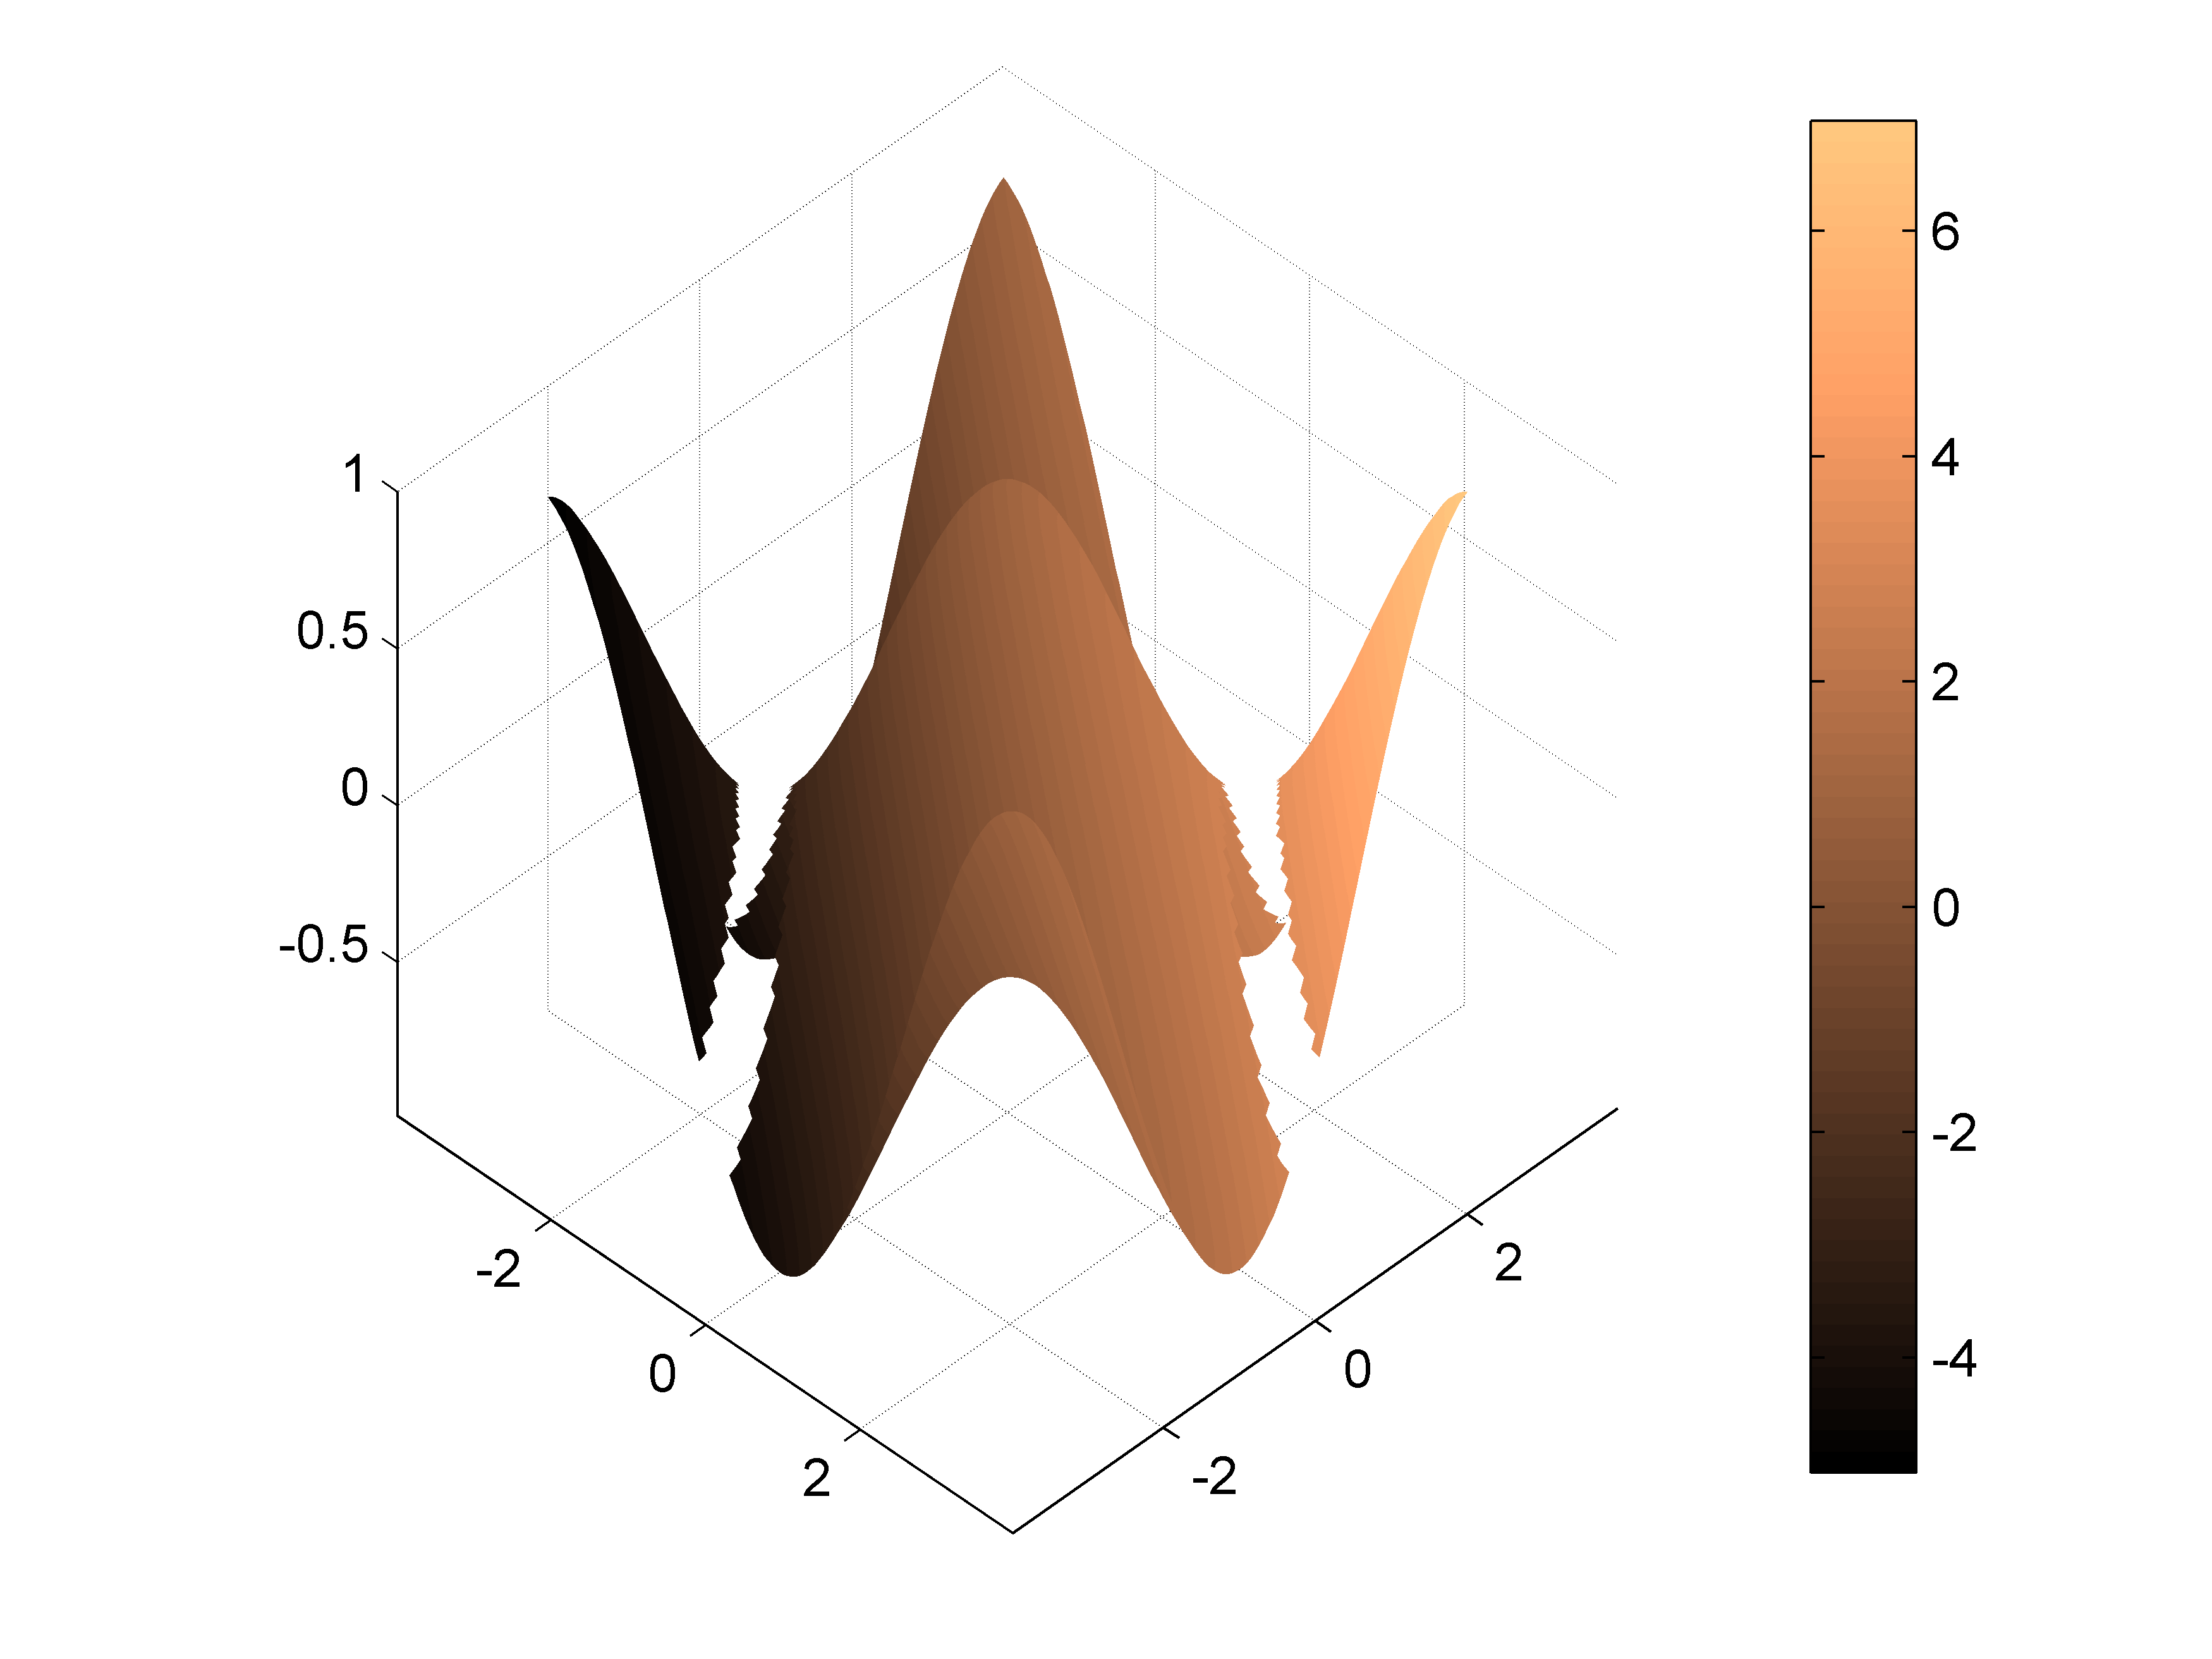
\includegraphics[width=300pt]{./Imagenes/3d7.png}

\paragraph{Ejemplo 3}:
\begin{lstlisting}[language=Matlab]
>> [X,Y]=meshgrid(-3:0.2:3); Z=exp(-X.^2-Y.^2);
>> surf(X,Y,Z, gradient(Z)), shading interp, colorbar
\end{lstlisting}
\includegraphics[width=300pt]{./Imagenes/3d8.png}

\paragraph{Ejemplo 4}:
\begin{lstlisting}[language=Matlab]
>> [X,Y]=meshgrid(-3:0.2:3); Z=exp(-X.^2-Y.^2);
>> surf(X,Y,Z,gradient(Z)), shading interp, alpha(0.6)
\end{lstlisting}
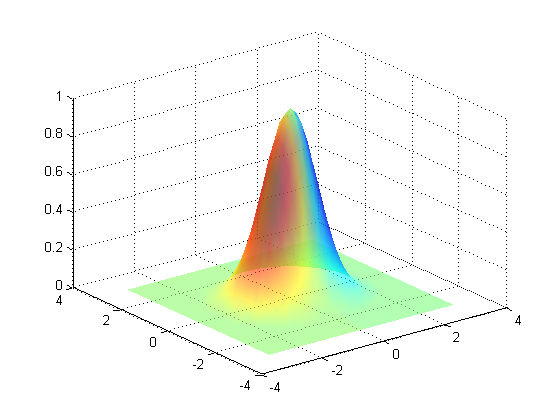
\includegraphics[width=300pt]{./Imagenes/3d9.png}

\section{Curvas de intersección entre dos superficies}

Existen muchos casos donde no se puede visualizar la curva que resulta de la intersección de 
dos superficies. Ejemplos:

\begin{enumerate}
\item La intersección de los cilindros: $z=x^{2}$ , $z=4-y^{2}$ es una curva en el espacio. Vamos a representar las dos superficies y luego su curva intersección. Gráfica de las superficies 

\begin{lstlisting}[language=Matlab]
>> [x,y]=meshgrid(-2:0.1:2); 
>> z=x.^2; mesh(x,y,z) 
>> hold on 
>> z=4-y.^2;
>> mesh(x,y,z)
\end{lstlisting}
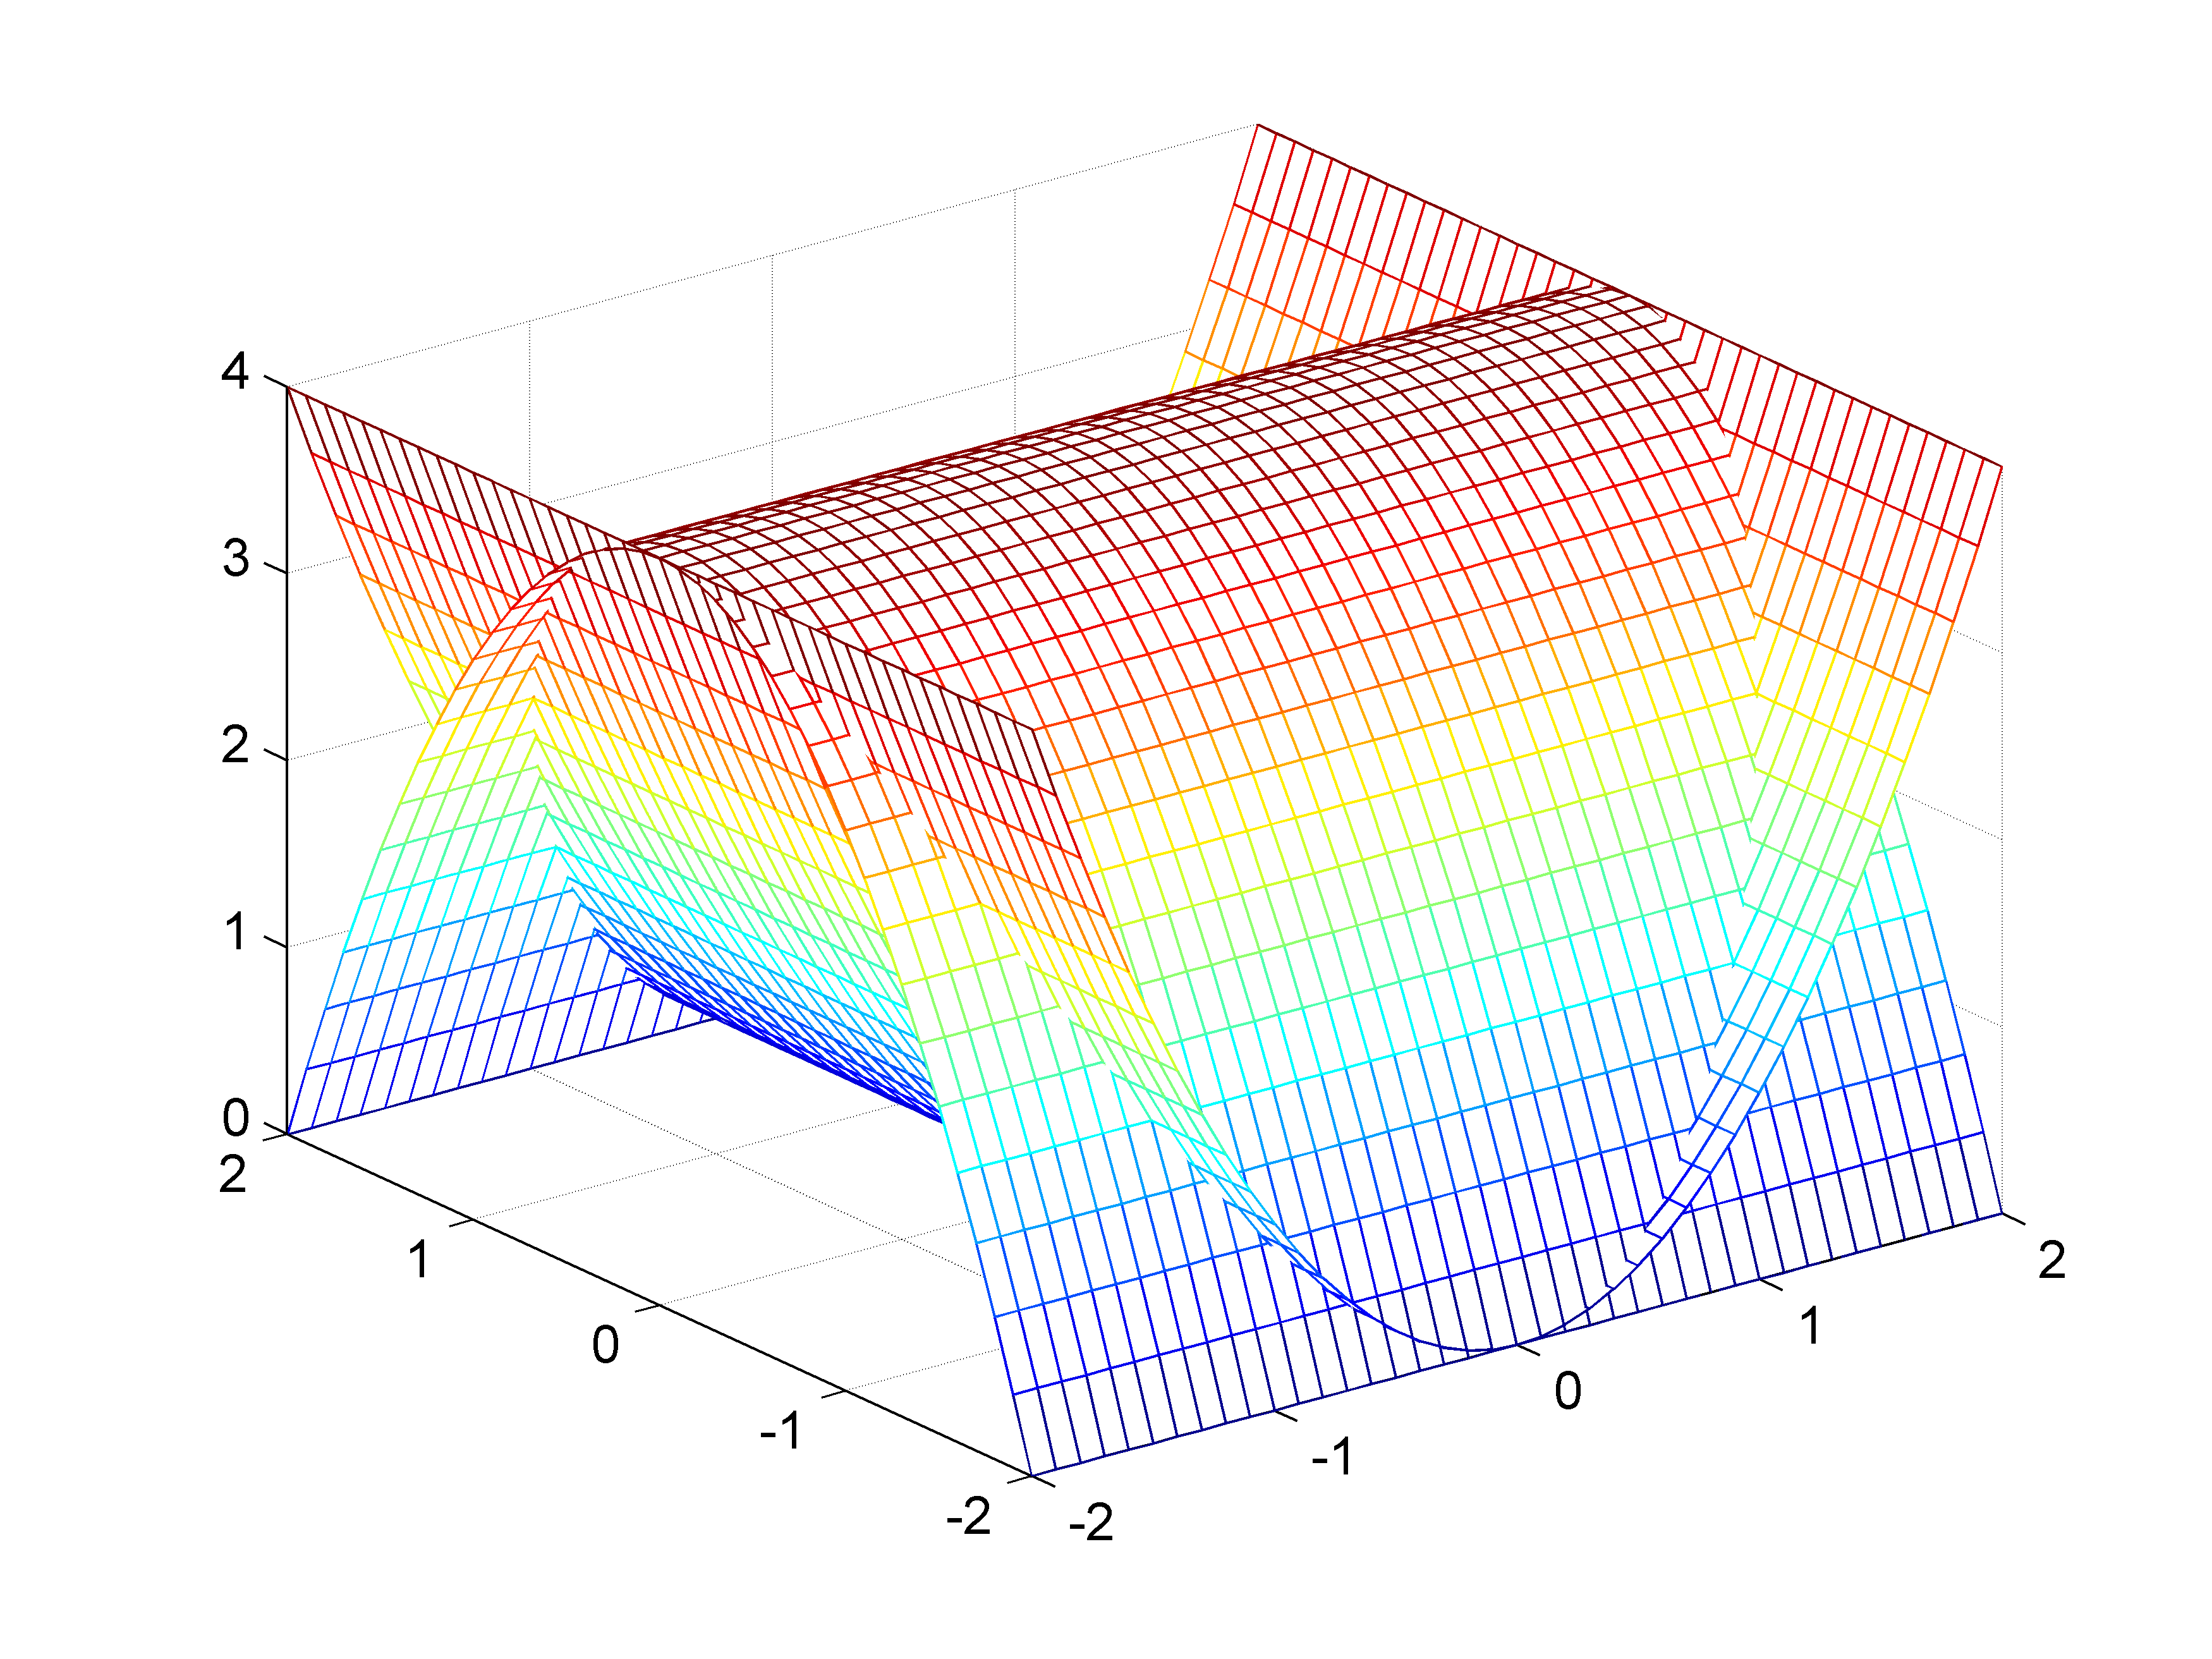
\includegraphics[width=300pt]{./Imagenes/superficies1.png}


Ahora vamos a generar el gráfico de la curva de intersección:
\begin{lstlisting}[language=Matlab]
>> t=0:pi/32:2*pi;
>> u=2*cos(t);
>> v=2*sin(t);
>> w=4*(cos(t)).^2;
>> plot3(u,v,w,'r')
\end{lstlisting}
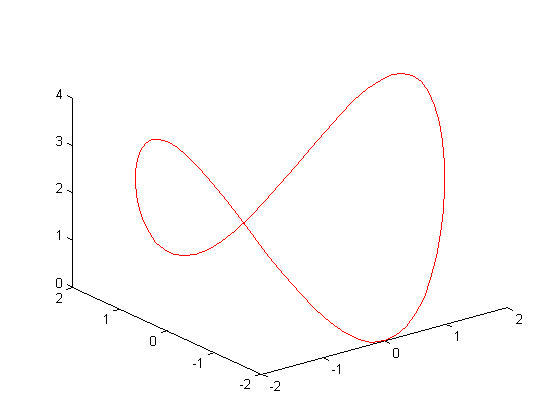
\includegraphics[width=300pt]{./Imagenes/superficies2.png}

Para obtener la proyección de esta curva al plano XY, reemplazar w: 
\begin{lstlisting}[language=Matlab]
>> t=0:pi/32:2*pi;
>> u=2*cos(t);
>> v=2*sin(t);
>> w=0*ones(1,65);
>> plot3(u,v,w,'r')
\end{lstlisting}

\item Las dos superficies $S_{1} : z=x^{2}+y^{2}$, $S_{2} : z=2+y$ determinan una curva. Halle las ecuaciones paramétricas de dicha curva y luego representar. Proyectando la curva al plano XY, esto es, igualando las ecuaciones se obtiene $x^{2} + (y-1/2)^{2} = \dfrac{9}{4}$

Ecuaciones paramétricas de la curva:
$$ x(t) = (3/2)cos(t) $$
$$ y(t) = (3/2)sin t+(1/2) $$
Si reemplazamos $y(t)$ en $z(t)$, se tiene $z(t)=\dfrac{5}{2}+(\dfrac{3}{2})sin(t) $

\begin{lstlisting}[language=Matlab]
>> [x,y]=meshgrid(-2:0.1:2);
>> z=x.^2+y.^2;
>> mesh(x,y,z)
>> hold on
>> z=2+y;
>> mesh(x,y,z)
>> t=0:pi/32:2*pi;
>> u=1.5*cos(t);
>> v=1.5*sin(t)+0.5;
>> w=2.5*ones(1,65)+1.5*sin(t);
>> plot3(u,v,w,'r')
\end{lstlisting}
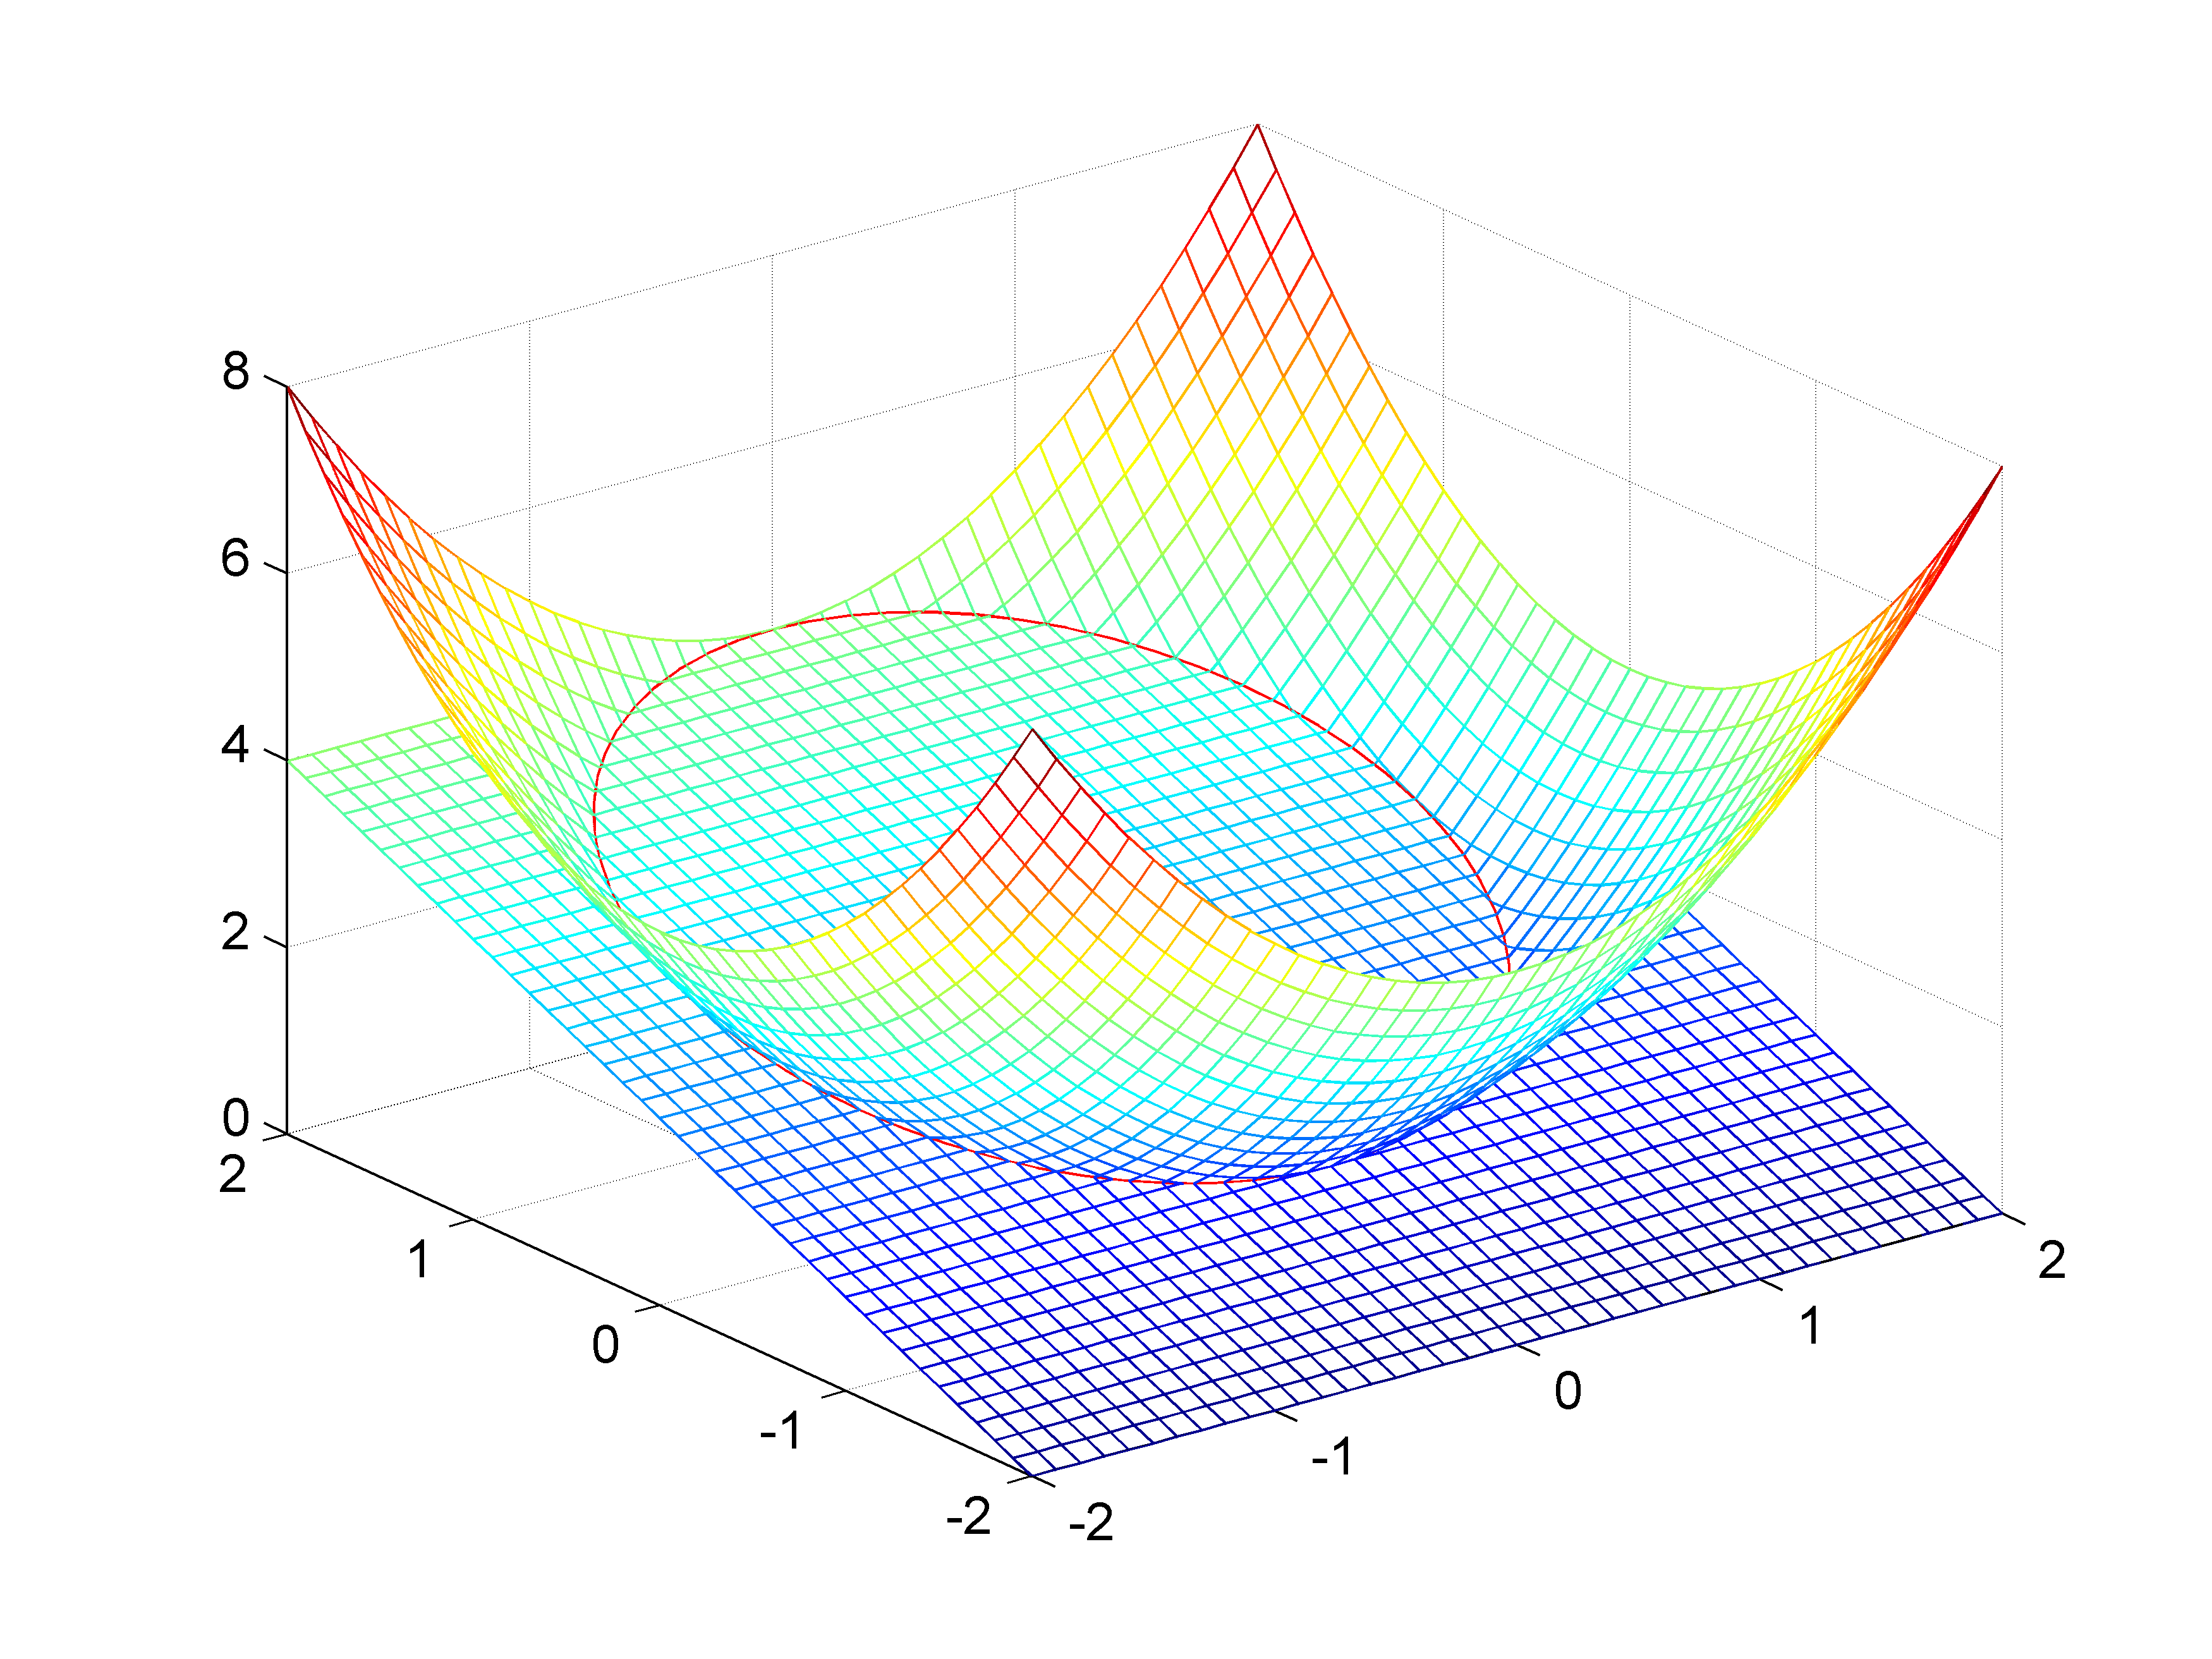
\includegraphics[width=300pt]{./Imagenes/superficies4.png}

\end{enumerate} 

\section{Curvas de nivel}

Sea $S$ una superficie representada por $z=f(x;y)$. La importancia de las curvas de nivel estriba en que trazando un número adecuado de ellas, podemos obtener una buena descripción de la superficie. A continuación se expone un ejemplo de como hallar las curvas de nivel:

\begin{enumerate}
\item Las curvas de nivel de la superficie $S: z = f(x,y) = 4^{2} + y^{2}$ son familias de elipses concentricas en el origen de coordenadas con semiejes  $\sqrt{k}/2$ y  $\sqrt{k}$, con $k>0$. 

$$ 4x^{2}+y^{2} = k \Rightarrow \dfrac{x^{2}}{\frac{k}{4}} + \dfrac{y^{2}}{k} = 1 $$

Gráfica de la superficie y algunas curvas de nivel:
\begin{lstlisting}[language=Matlab]
>> [x,y]=meshgrid(-2:.1:2); 
>> z=4*x.^2+y.^2; 
>> contour(x,y,z,10)
>> contour3(x,y,z,10) 
>> meshc(x,y,z)
\end{lstlisting}
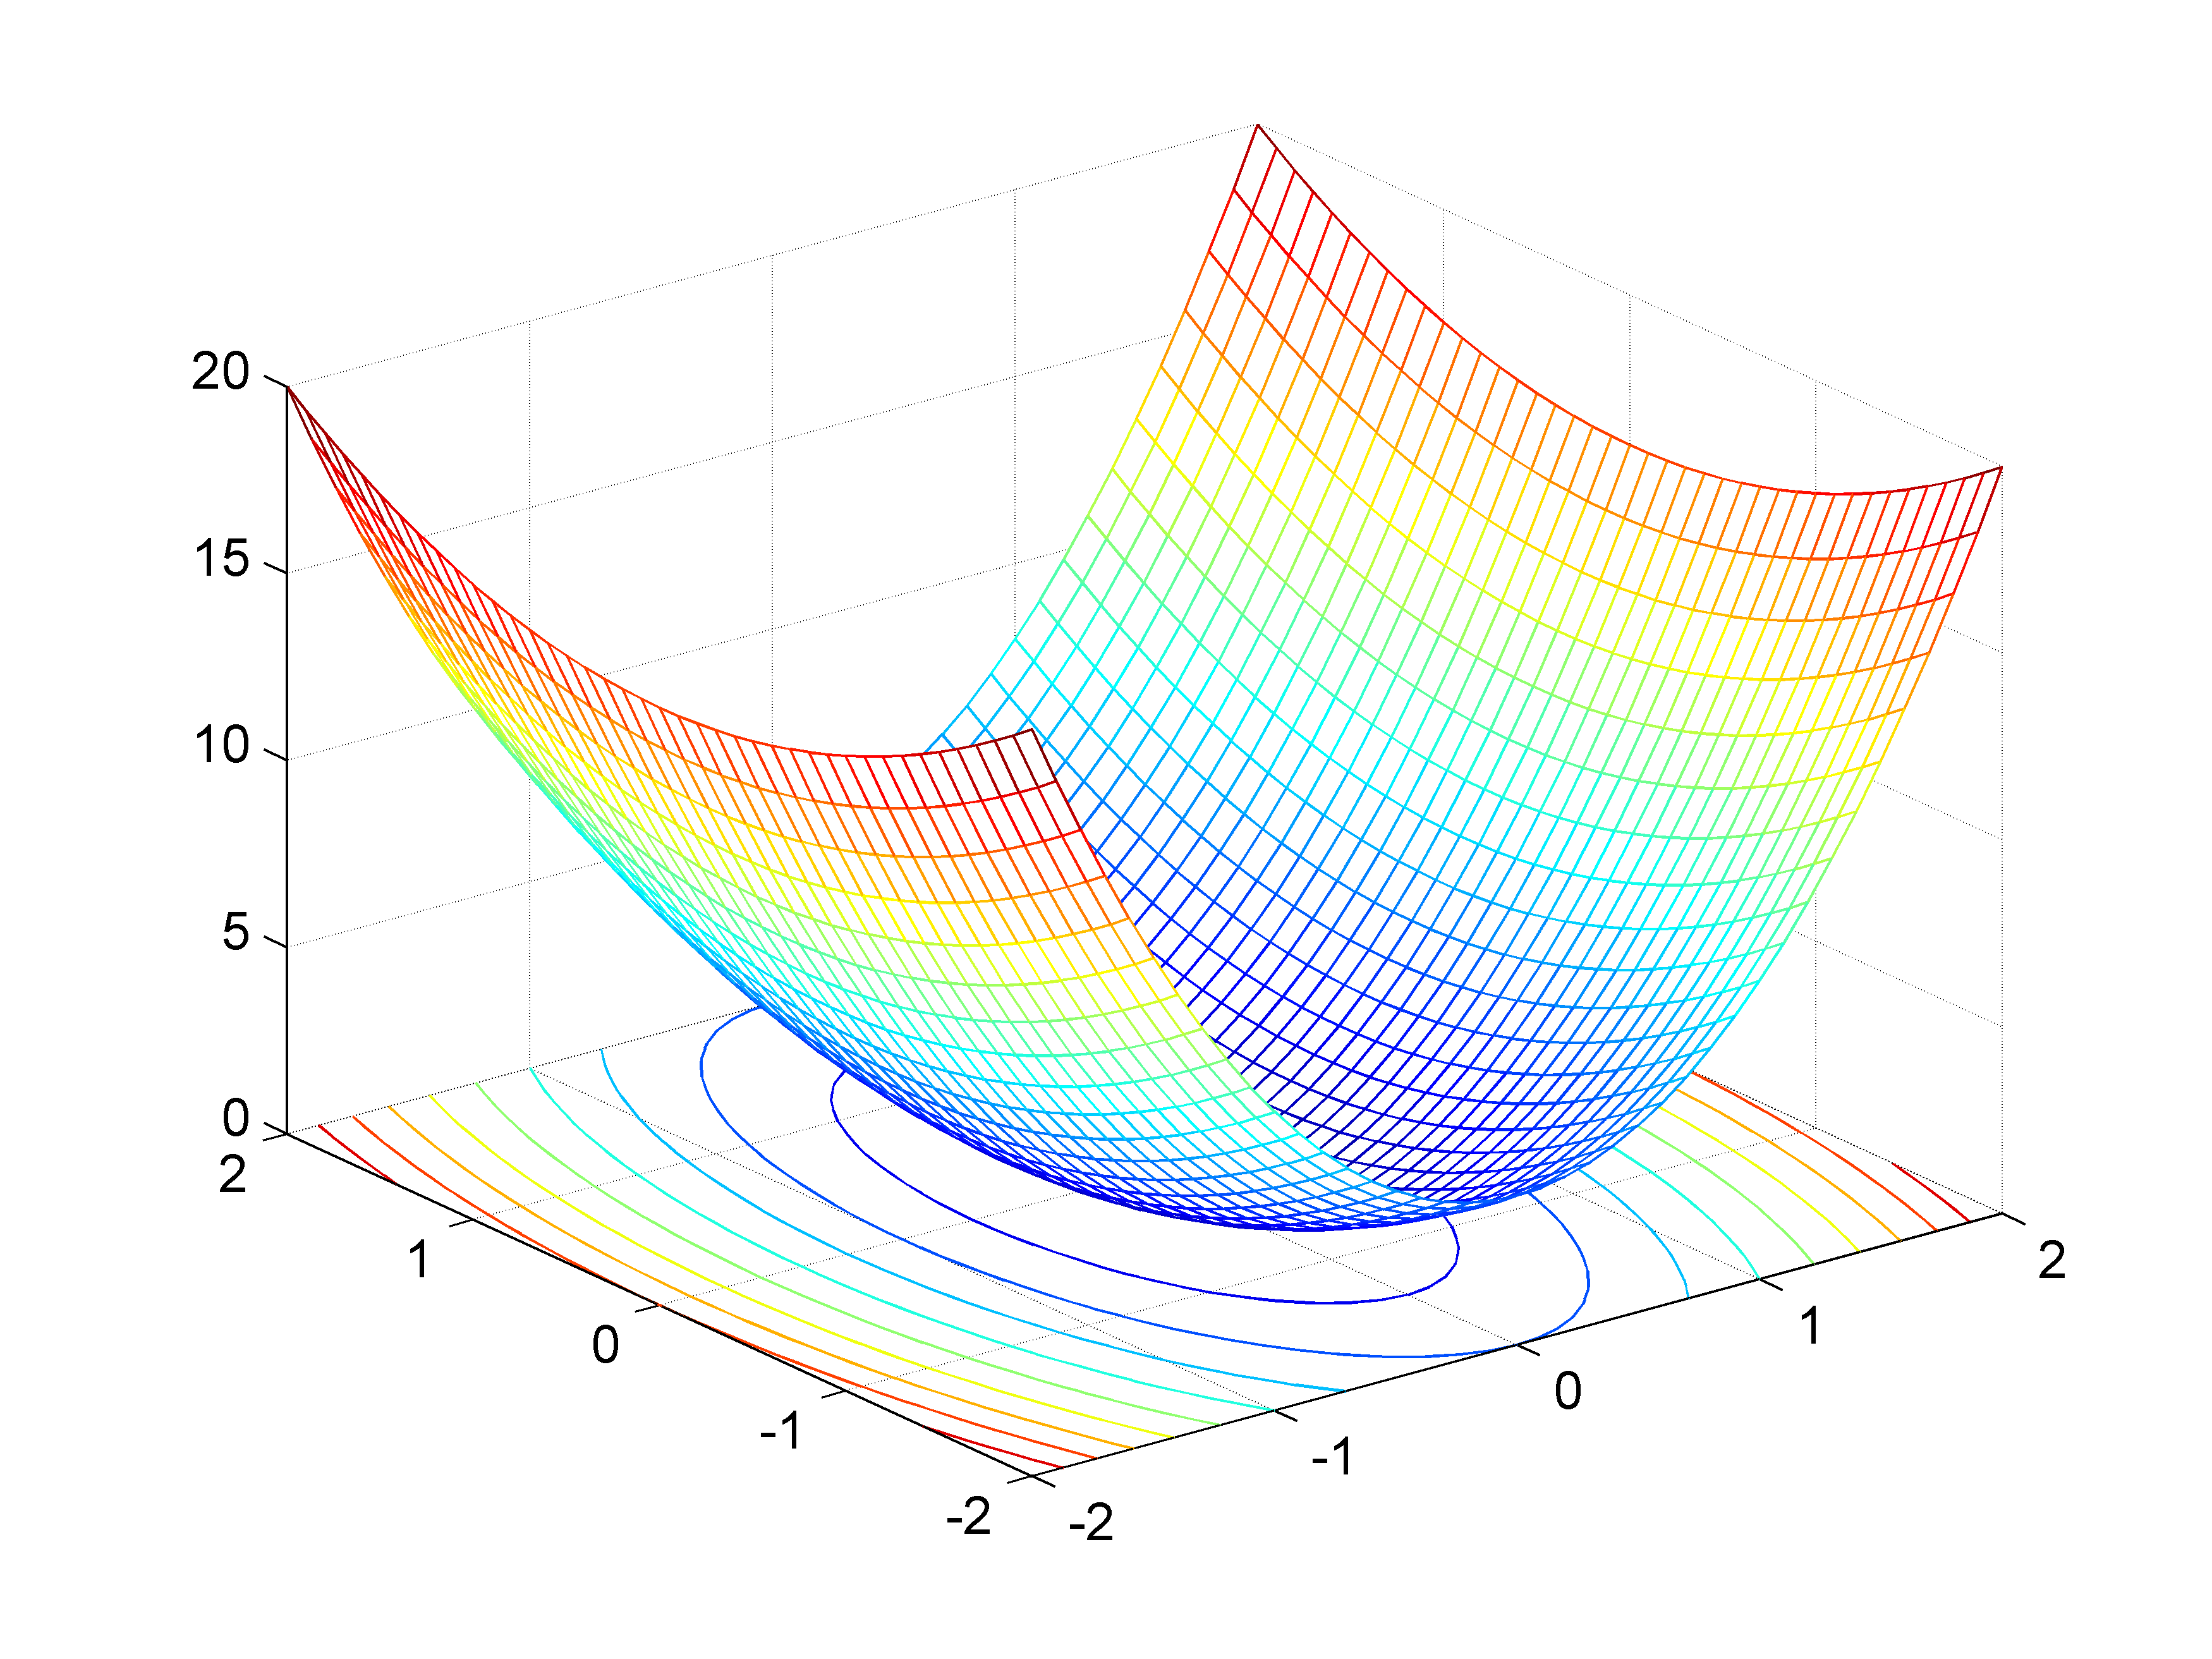
\includegraphics[width=300pt]{./Imagenes/curvanivel1.png}

La superficie y las curvas de nivel están generadas con \textbf{meshc}.
\end{enumerate} 

\section{Superficies de revolución}

Una superficie de revolución es la engendrada por la rotación de una curva plana en torno de 
una recta fija contenida en el plano de la curva. La curva plana se llama \textit{generatriz}, y la recta fija \textit{eje de revolución} o, simplemente eje de la superficie. Cualquier posición de la generatriz se llama \textit{meridiano}, y cada circunferencia descrita por un punto de la generatriz se llama \textit{paralelo} de la superficie.

Para determinar la ecuación de una superficie de revolución, no se pierde generalidad si se toma la generatriz en uno de los planos coordenados y como eje de revolución a uno de los ejes 
coordenados contenidos en ese plano.

Sea G la curva generatriz contenida en el semiplano superior YZ, $G : z = f(y) \geqslant 0 $ y el eje de revolución el eje Z. Sea $P(x;y;z)$, un punto cualquiera de la superficie. El paralelo que pasa por P corta a G en un punto del plano YZ, digamos $Q(0;y^{'};z^{'})$, y su centro $A(0;0;z^{'})$ está sobre el eje de revolución, el eje Z.

Por ser radios del mismo paralelo,$\mid AP \mid$ = $\mid AQ \mid$ entonces
$ z^{'}= \pm \sqrt{x^{2} + y^{2}}$. Además, P y Q están en el mismo plano, entonces $z^{'}=z$. Como $Q \in G : z^{'}=f(y^{'})$.

Reemplazando $y^{'}$, $z^{'}$, en $z^{'} = f(y^{'})$ se obtiene la ecuación de la superficie de revolución $z = f(\sqrt{x^{2} + y^{2}})$.

Representaremos a las superficies de revolución como si fueran superficies paramétricas, 
considerando a \textbf{x} e \textbf{y} como parámetros.

\textbf{Ejemplo}: Sea la curva $C : z = y^{2}$ en el plano YZ. Si el eje de rotación es el eje Z, hallamos la ecuación de la superficie de revolución que genera C.

\textbf{Solución}: En el plano $z=z_{0}$ se encuentra un paralelo, cuyo centro es $A(0;0;z_{0})$. El punto $Q(0;y_{0};z_{0})$ es un punto que resulta de la intersección de C con el plano $z=z_{0}$. Si $P(x;y;z)$ es un punto arbitrario de la superficie que se encuentra en el paralelo entonces $\mid AP \mid$ = $\mid AQ \mid$ y esto implica que $\mid y_{0} \mid = \sqrt{x^{2} + y^{2}}$. Como $Q \in G : z_{0} = y_{0}^{2}$, entonces la ecuación de la superficie es $ S : z = x^{2}+y^{2}$.

\subsection{Superficies de revolución definidas en MATLAB}

Se pueden representar directamente ciertas superficies de revolución conocidas como esferas, 
cilindros, elipsoides, etc.

\subsubsection{Esfera}

Su gráfica se obtiene con el comando \textbf{sphere(n)}, donde \textbf{n} es el número de puntos en los que queda dividido tanto el ecuador de la esfera como el meridiano principal. A raíz de esa división se representa la esfera con \textbf{n} paralelos y \textbf{n} meridianos. Con \textbf{sphere(20)} se obtiene la esfera con 20 paralelas y 20 meridianos.

\begin{lstlisting}[language=Matlab]
>> sphere(20)
\end{lstlisting}
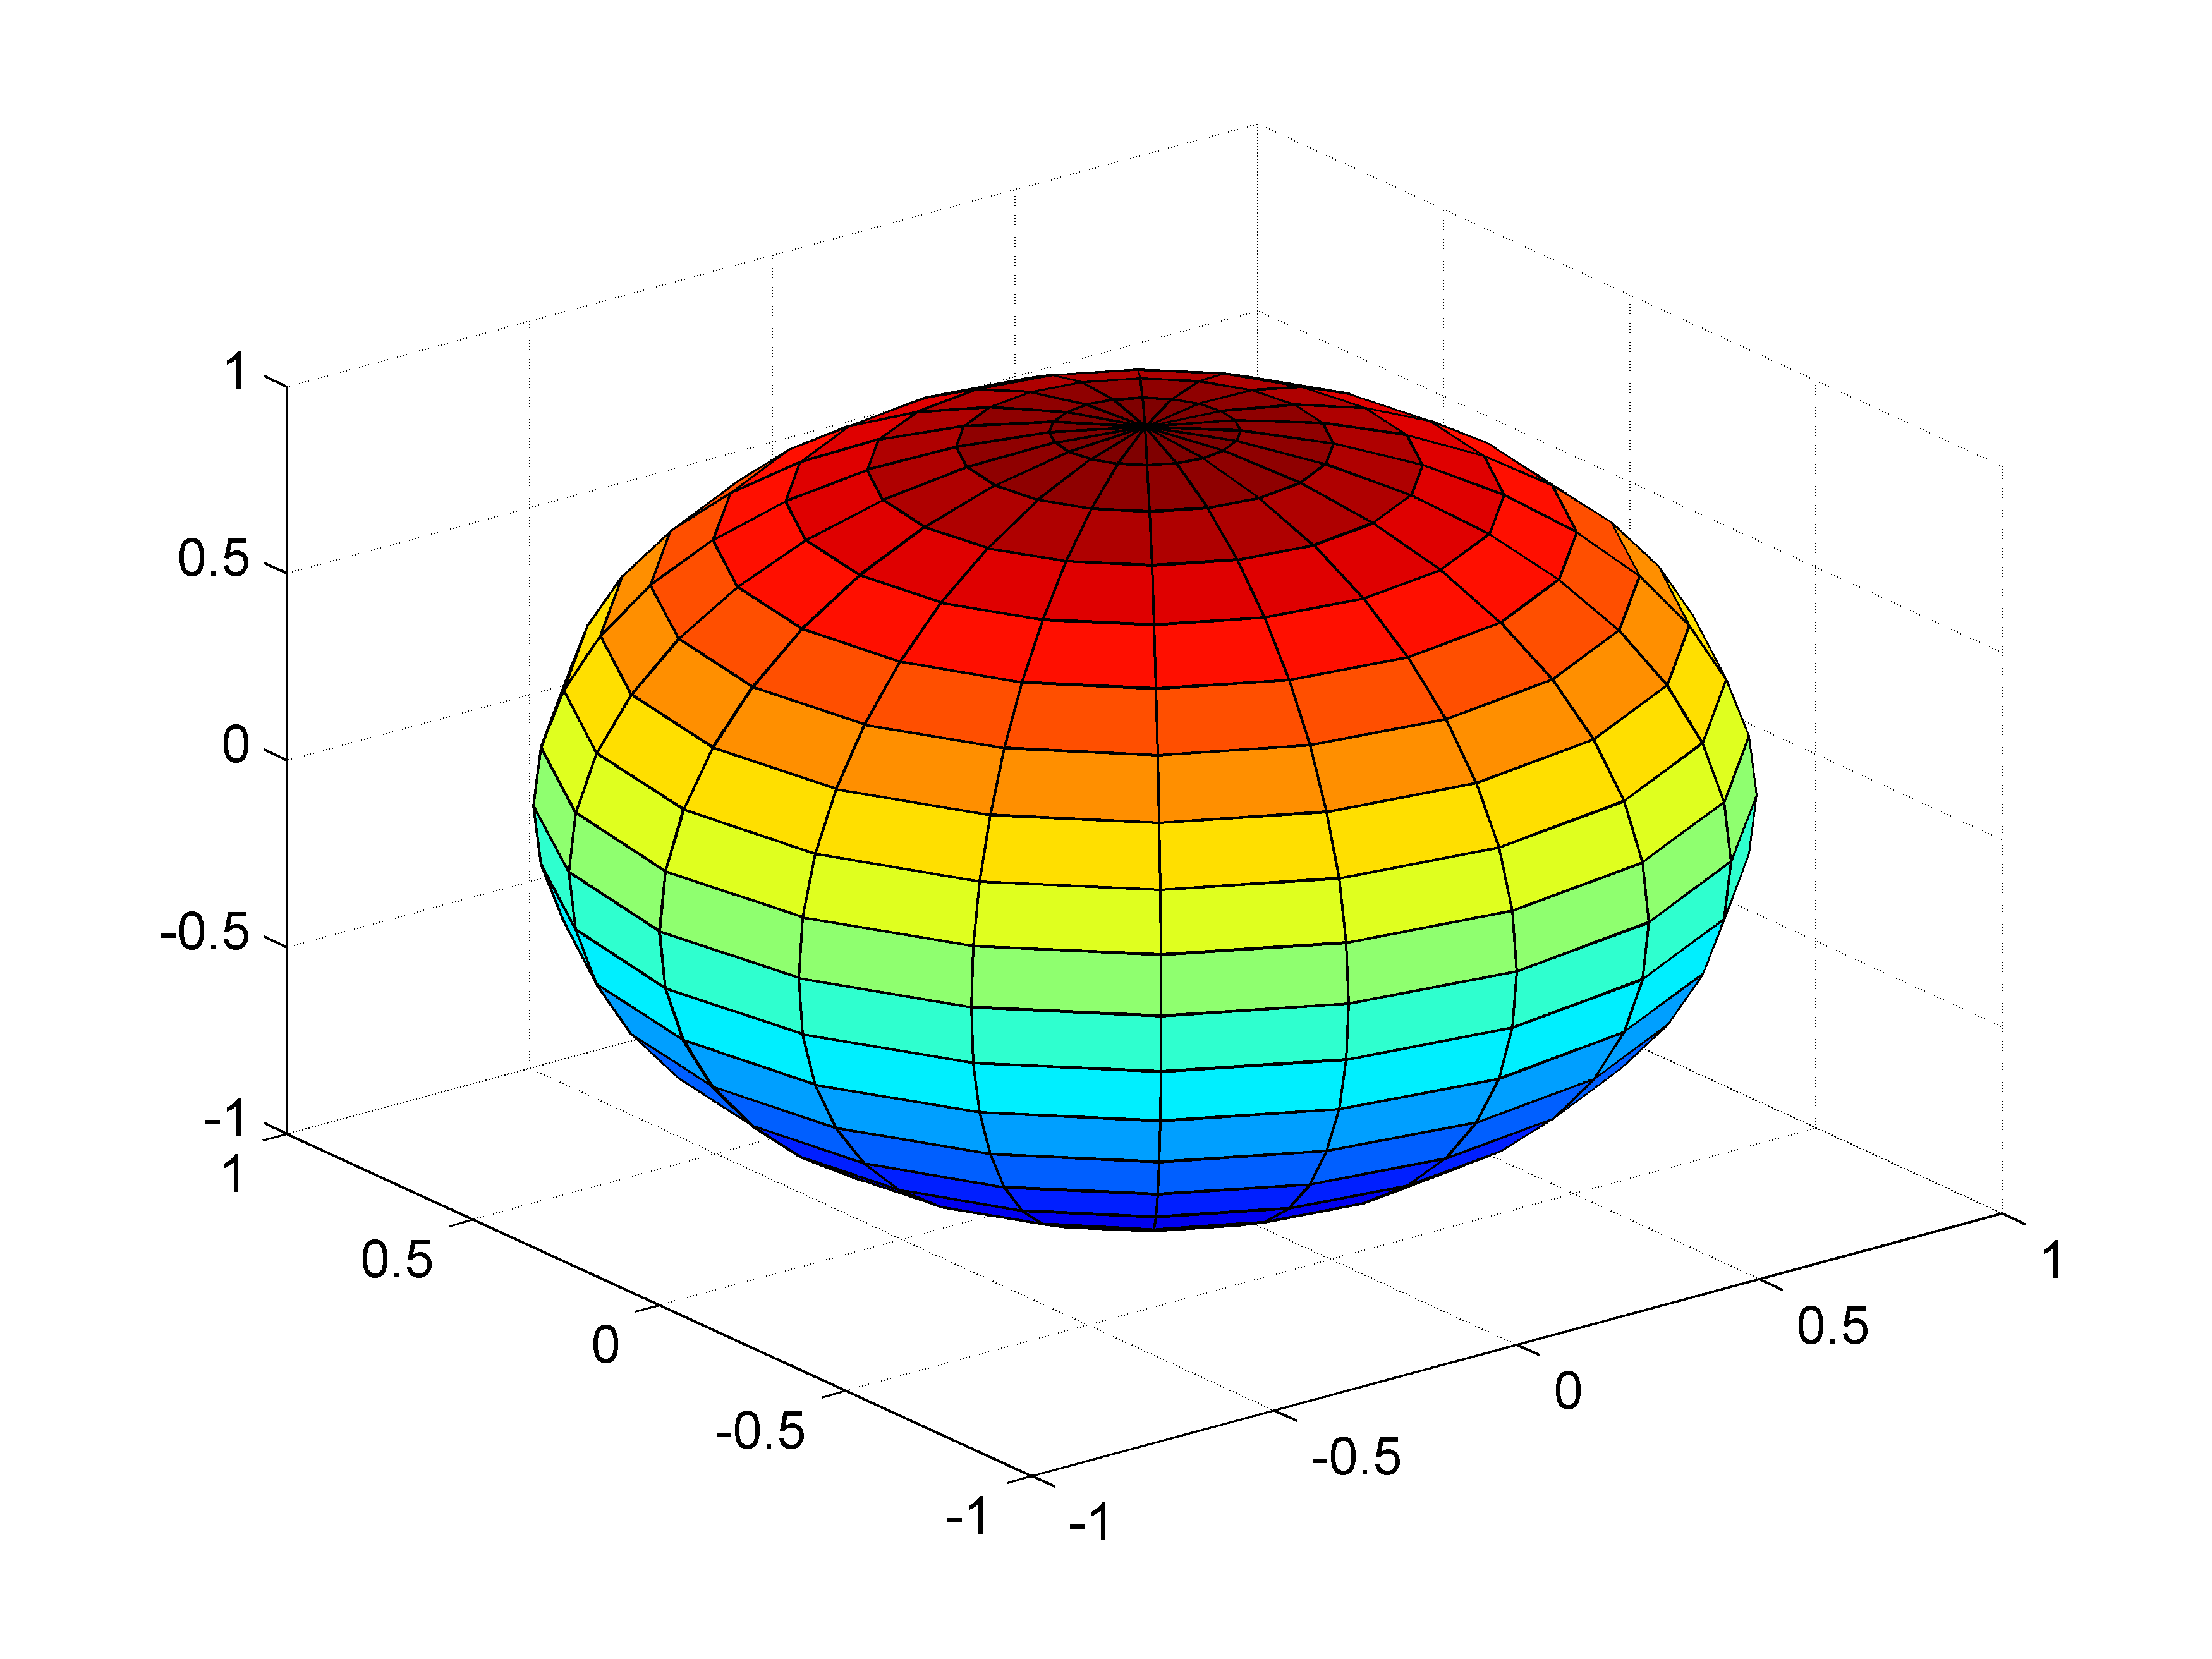
\includegraphics[width=200pt]{./Imagenes/esfera1.png}

Vectores normales a una esfera:
\begin{lstlisting}[language=Matlab]
>> [x,y,z]=sphere(20); 
>> surfnorm(x,y,z)
\end{lstlisting}
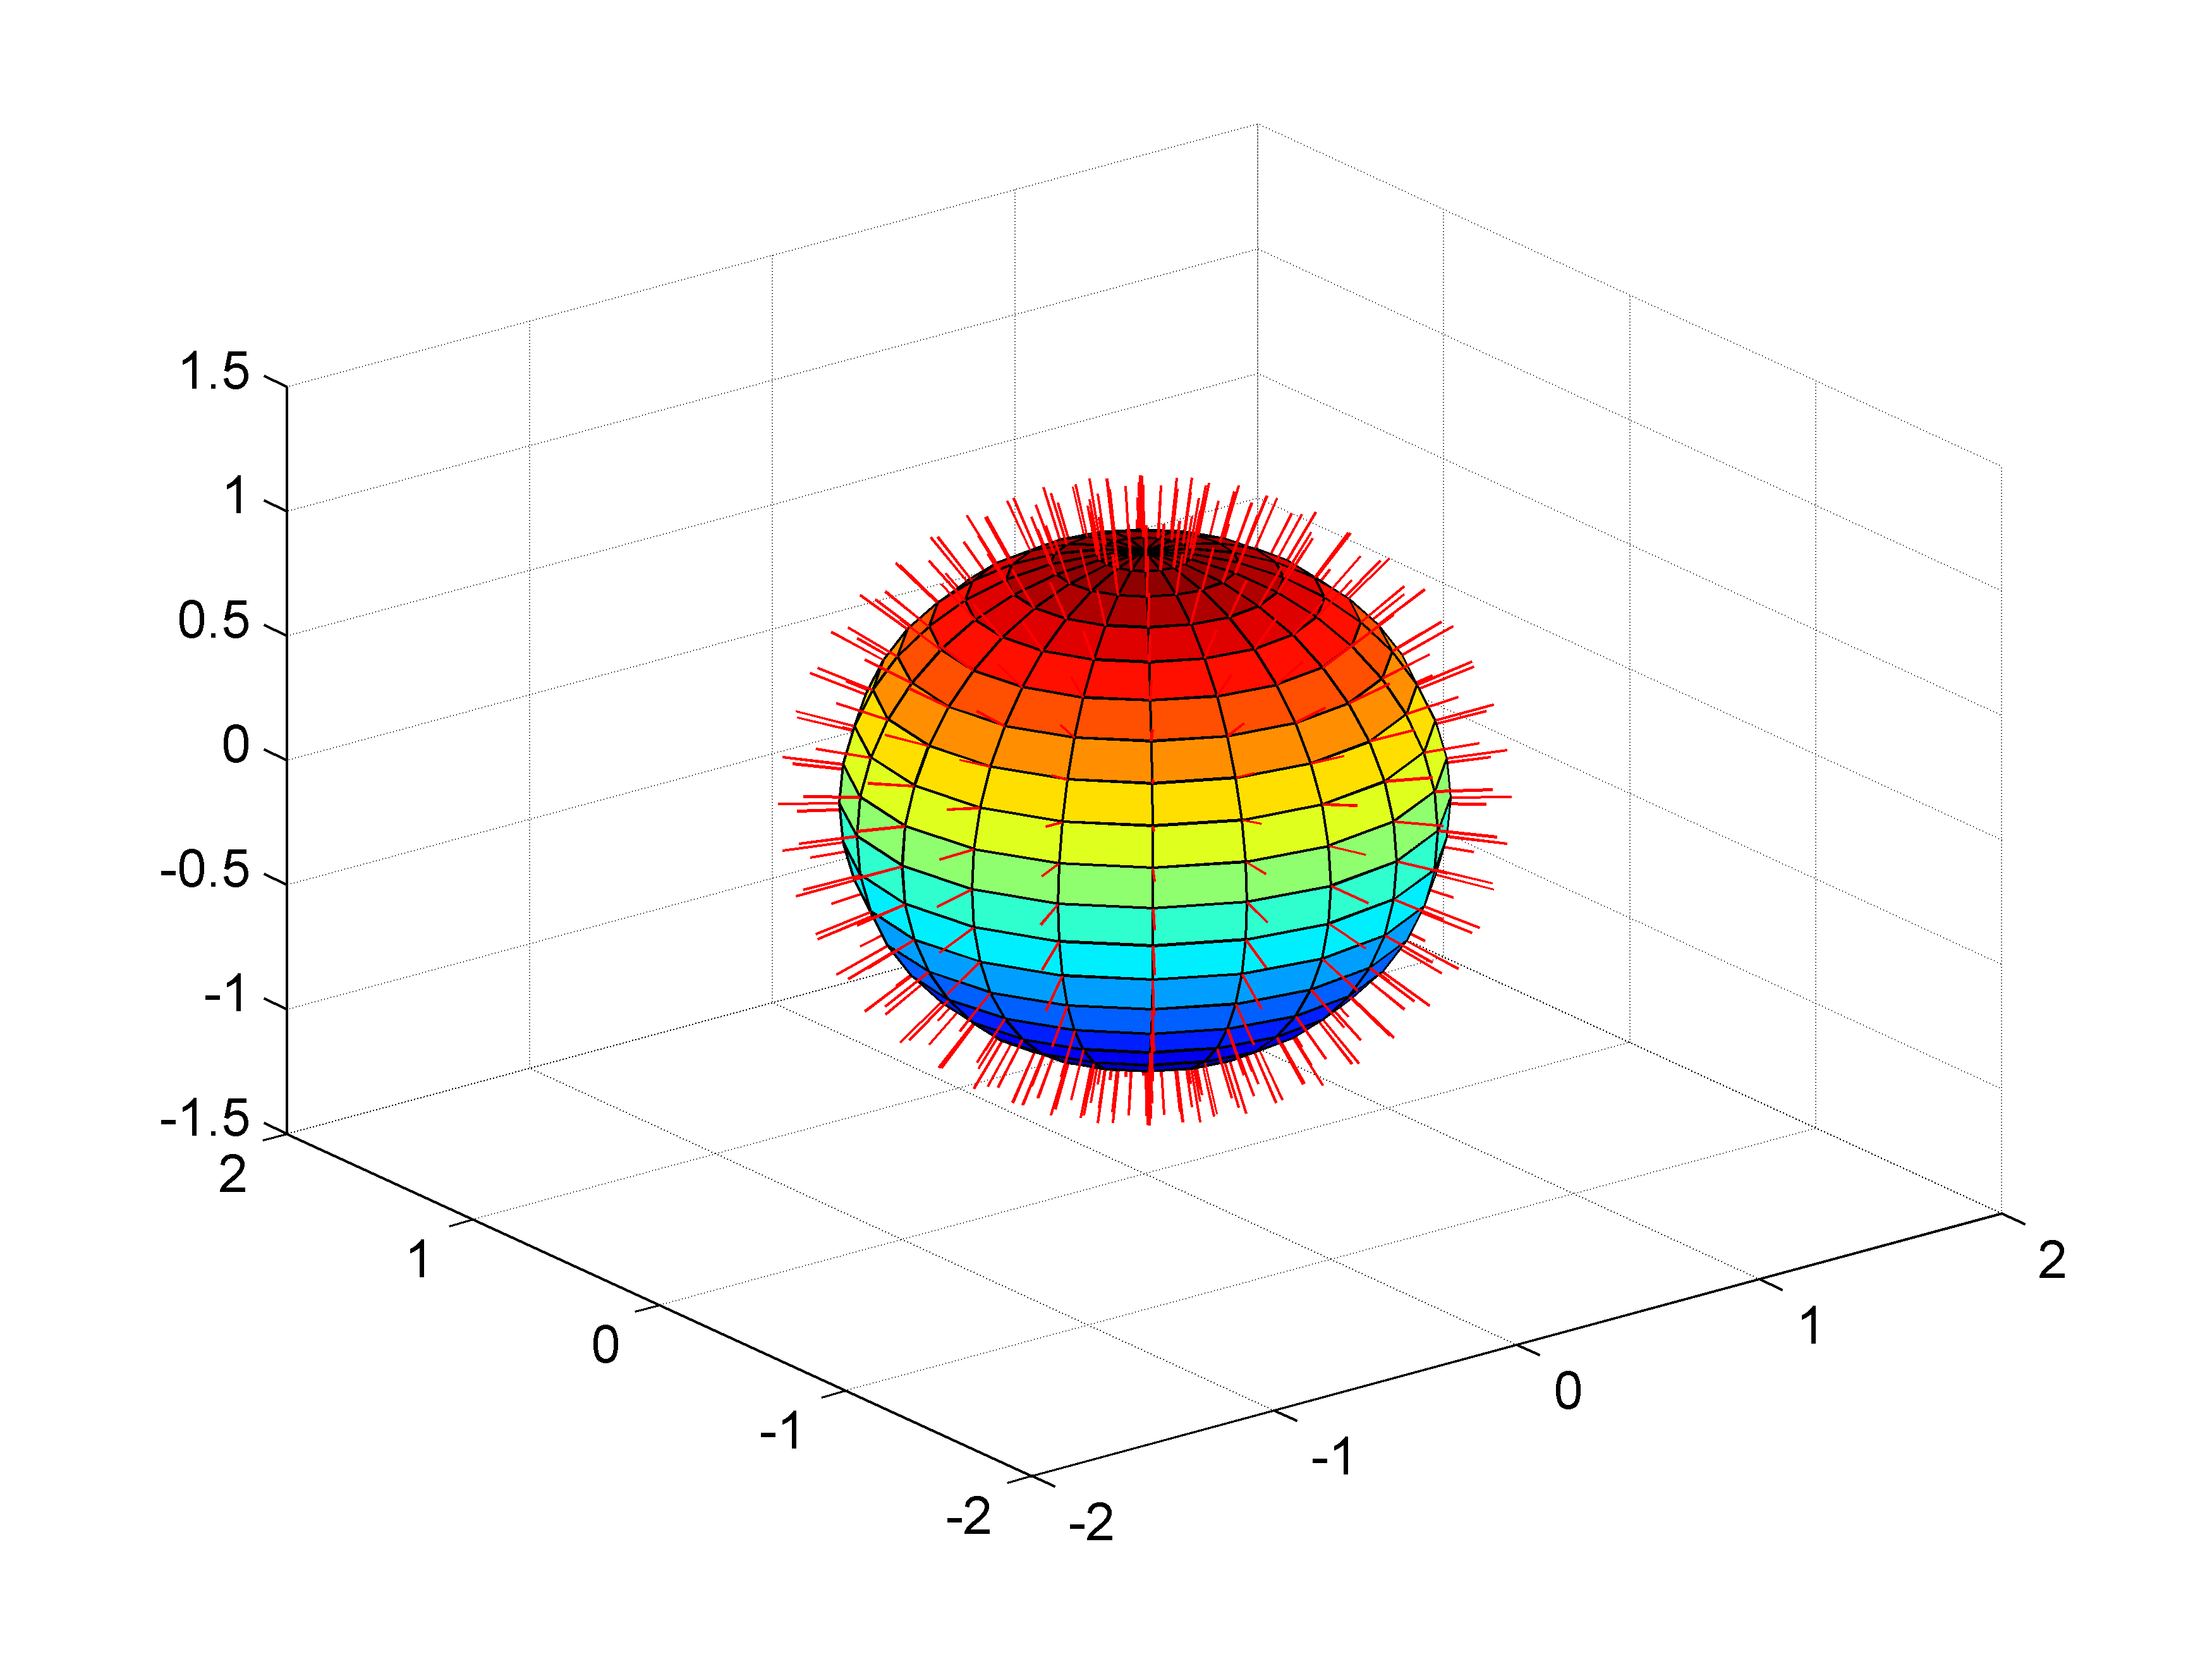
\includegraphics[width=300pt]{./Imagenes/esfera2.png}

\subsubsection{Cilindro}

Se representa mediante el comando \textbf{cylinder}. Este comando \textbf{cylinder(R, n)} genera automáticamente un cilindro de revolución de radio R y n segmentos generatrices. En este caso, la circunferencia de la base del cilindro es dividido en n puntos, por donde pasan dichas generatrices paralelas al eje del cilindro.
\begin{lstlisting}[language=Matlab]
>> cylinder(10,90)
\end{lstlisting}
\includegraphics[width=300pt]{./Imagenes/cilindro.png}


\section{Superficies paramétricas}

Una superficie $S$ puede ser representada por una función vectorial $r(u,v) = (x, y, z)$, donde $(u,v) \in D$ en el plano. Las funciones x, y, z dependen de los parámetros u y v. A las ecuaciones:
$$x=x(u,v)$$
$$y=y(u,v)$$
$$z=z(u,v)$$
se denomina ecuaciones paramétricas de $S$.

\textbf{Definición}: Un subconjunto $S$ de $\Re^{3}$ se denomina una superficie regular si para cada p en S existe una vecindad $ V \subset \Re^{3} $ de p, un abierto $ U \subset \Re^{2} $ y una bisección $\varphi : U \longrightarrow V \cap S$ con algunas propiedades que no vamos a ver en este curso. Vamos a ver un ejemplo de como representar una superficie según sus ecuaciones paramétricas.

\begin{enumerate}

\item Superficie de revolución con perfil la curva definida por $r= \sqrt{t}$ , $t \in [0,2]$
\begin{lstlisting}[language=Matlab]
>> t=linspace(0,2,20); 
>> r=sqrt(t); 
>> cylinder(r) 
>> xlabel('t');ylabel('r(t)');zlabel('z(t,r)')
\end{lstlisting}
\includegraphics[width=300pt]{./Imagenes/supfparam1.png}


\item Superficie de revolución de perfil $2 + cos(t)$
\begin{lstlisting}[language=Matlab]
>> t = 0:pi/10:2*pi; 
>> [X,Y,Z] = cylinder(2+cos(t)); 
>> surf(X,Y,Z) 
>> axis square 
>> xlabel('x');ylabel('y');zlabel('z')
\end{lstlisting}
\includegraphics[width=300pt]{./Imagenes/supfparam2.png}

\item Cilindro como superficie de revolución
\begin{lstlisting}[language=Matlab]
>> r=(0:0.1:2*pi)'; 
>> t=-pi:0.1:2*pi; 
>> X=cos(r)*sin(t); 
>> Y=sin(r)*sin(t); 
>> Z=ones(1,size(r))'*t; 
>> surf(X,Y,Z) 
>> axis square
\end{lstlisting}
\includegraphics[width=300pt]{./Imagenes/cilindsupf.png}

\item Toroide: Considere en $\Re^{3}$ la circunferencia $C={(x,y,z):(y-2)^{2}+z^{2}=1, x=0}$. 
Al rotar C alrededor del eje Z se obtiene el toro. Una parametrización para esta superficie está dada por $\varphi(u,v) = (cos u(2+cos v),sin u(2+cos v),sin v), 0 \leq u \leq 2\pi ,0 \lq v \leq 2\pi$. 
La gráfica del toro se obtiene con la secuencia de comandos. 

\begin{lstlisting}[language=Matlab]
>> u=linspace(0,2*pi,41); v=u; 
>> [U,V]=meshgrid(u,v); 
>> X=cos(U).*(2+cos(V)); 
>> Y=sin(U).*(2+cos(V)); 
>> Z=sin(V); 
>> surf(X,Y,Z) 
>> axis([-3 3 -3 3 -1 1])
\end{lstlisting}
\includegraphics[width=300pt]{./Imagenes/toroide.png}


\item Superficie "Tobogán", variación a la del toro. 

\begin{lstlisting}[language=Matlab]
>> u=(0:pi/8:4*pi)'; 
>> v=0:pi/16:2*pi;
>> X=cos(u)*(2+sin(v)); 
>> Y=sin(u)*(2+sin(v)); 
>> Z=u*ones(size(v))+ones(size(u))*cos(v); 
>> mesh(X,Y,Z)%surfl(X,Y,Z)%surf(X,Y,Z) 
>> axis([-4 4 -4 4 0 10]) 
\end{lstlisting}
\includegraphics[width=300pt]{./Imagenes/tobogan.png}


\item El unicornio
\begin{lstlisting}[language=Matlab]
>> u=linspace(0,6*pi,60);
>> v=linspace(0,2*pi,60);17
>> [u,v]=meshgrid(u,v);
>> x=2*(1-exp(u/(6*pi))).*cos(u).*cos(v/2).^2;
>> y=2*(-1+exp(u/(6*pi))).*sin(u).*cos(v/2).^2;
>> z=1-exp(u/(3*pi))-sin(v)+exp(u/(6*pi)).*sin(v);
>> mesh(x,y,z)
\end{lstlisting}
\includegraphics[width=300pt]{./Imagenes/unicornio.png}


\item La Cinta de Möbius. Es una superficie que se puede construir a partir de una tira de papel de forma rectangular ABCD. Torciendo la tira, una sola vez, de manera que se haga 
coincidir el vértice A con el vértice C y el vértice B con el vértice D obteniendo la 
superficie mencionada.

Se genera con la siguiente función vectorial 
$$r(u,v) = [\dfrac{v}{2}*sin(\frac{u}{2}),(1 + \dfrac{v}{2}*cos(\frac{u}{2}))*sin(u),(1 + \dfrac{v}{2}*cos(\frac{u}{2}))*cos(u)]$$ donde $0 \leq u \leq 2\pi ,-1 \lq v \leq 1$

\begin{lstlisting}[language=Matlab]
>> u=linspace(0,2*pi,30);
>> v=linspace(-1,1,15);
>> [u,v]=meshgrid(u,v);
>> z=(1+v/2.*cos(u/2)).*cos(u);
>> y=(1+v/2.*cos(u/2)).*sin(u);
>> x=v/2.*sin(u/2);
>> surf(x,y,z)
\end{lstlisting}
\includegraphics[width=300pt]{./Imagenes/cinta.png}

\end{enumerate}
\chapter{Creación de animaciones}

Para preparar pequeñas películas o movies se pueden utilizar las funciones $movie$, $moviein$ y $getframe$. Una película se compone de varias imágenes, denominadas frames. La función \textbf{getframe}  devuelve un vector columna con la información necesaria para reproducir la imagen que se acaba de representar en la figura o ventana gráfica activa, por ejemplo con la función plot. El tamaño de este vector columna depende del tamaño de la ventana, pero no de la complejidad del dibujo. La función \textbf{moviein(n)} reserva memoria para almacenar \textbf{n} frames. La siguiente lista de comandos crearía una película de 17 imágenes o frames, que se almacenarán como las columnas de la matriz M:

\begin{lstlisting}[language=Matlab]
>> M = moviein(170);
>> x=[-2*pi:0.1:2*pi]';
>> for j=1:170
>> y=sin(x+j*pi/8);
>> plot(x,y);
>> M(:,j) = getframe;
>> end 
\end{lstlisting}

Una vez creada la película se puede representar el número de veces que se desee con el comando \textbf{movie}. Por ejemplo, para representar 10 veces la película anterior, a 15 imágenes por segundo,habría que ejecutar el comando siguiente (los dos últimos parámetros son opcionales): 

\begin{lstlisting}[language=Matlab]
movie(M,10,15)
\end{lstlisting}

Los comandos \textbf{moviein}, \textbf{getframe} y \textbf{movie} tienen posibilidades adicionales para las que puede consultarse el Help correspondiente. Hay que señalar que en \textbf{MATLAB} no es lo mismo un movie que una animación. Una animación es simplemente una ventana gráfica que va cambiando como consecuencia de los comandos que se van ejecutando. Un movie es una \textit{animación grabada o almacenada en memoria previamente}.

Las películas pueden generarse de dos maneras: guardando fotogramas en el disco (normalmente utilizando print) y luego utilizar un programa externo para crear la película o mediante los comandos \textbf{getframe}, \textbf{movie}, de forma tal de que \textbf{MATLAB} genere un archivo de video.
\begin{lstlisting}[language=Matlab]
>> for k = 1:16 
>>    plot(fft(eye(k+16))) 
>>    axis equal 
>>    M(k) = getframe; 
>> end 
>> movie(M,1); %play the movie 
>> movie2avi(M,'mi_peli','fps',1); 
\end{lstlisting}
\chapter{Programación en Matlab}

Como ya hemos visto, Matlab es un programa diseñado especialmente para tratar datos matemáticos. Entre otras aplicaciones permite la programación, esto es, la creación de una serie de instrucciones que se ejecutaran cuando se las invoque. El código se guarda en archivos .M, que son interpretados cada vez que se ejecutan.

\section{Ejecución de archivos .m}

Solo hay que poner su nombre, sin la extension, en el Command Windows. Por ejemplo, si tenemos un archivo previamente creado que se ha guardado como ejemplo.m.\\

Edit es un editor donde podemos escribir instrucciones que no se ejecutan hasta que sean invocadas en la ventana principal.

Para crear un archivo .M nuevo basta con hacer clic sobre la representación de una hoja en blanco, que sirve para crear un nuevo archivo .m.\\

Una vez escrito el programa, se guarda con el nombre deseado (siempre y cuando no sea una “function”, ya que entonces hay que guardarlo con el mismo nombre) y la extension. Algunos comandos muy utilizados en archivos .M son:

\begin{itemize}
\item ECHO OFF - ECHO ON: muestran o ocultan respectivamente los comandos.
\item PAUSE: la ejecución del programa se detiene hasta dar a una tecla.
\item INPUT: permite que con el teclado metamos el valor de una variable, el formato en el que se usa se indica mas adelante en un ejemplo.
\item DISP: muestra el contenido de 1 variable sin mostrar su nombre o el texto introducido según la forma de utilizarlo. Los distintos formatos se muestran a continuación en un ejemplo.
\item RETURN: para el programa.
\end{itemize}

\section{Condiciones simples}

El diagrama muestra el formato de una condición simple:\\

\begin{center}
\includegraphics[width=200pt]{./Imagenes/condicionsimple.png}
\end{center}

A continuación, un código de ejemplo. La primera linea indica que si (y solo si) se cumple la condición dada, se va a realizar la sentencia 1. La tercera linea indica que si no se cumple la condición se realiza la sentencia 2. El end que aparece en la cuarta linea se utiliza para finalizar la bifurcación.

\begin{lstlisting}[language=Matlab]
if condicion
    sentencia 1
else sentencia 2
end
\end{lstlisting}

\paragraph{Ejemplo 1}

Crear un programa en el que se introduzcan dos números por el teclado y que nos diga cual es el mayor.

\begin{lstlisting}[language=Matlab]
a = input('Ingrese un numero')
b = input('Ingrese otro numero')
if a > b
    disp ('El primer numero es mayor que el segundo')
else 
    disp ('El segundo numero es mayor que el primero')
end
\end{lstlisting}

\section{Condiciones múltiples}

La sntaxis es de la siguiente forma:\\
\begin{lstlisting}[language=Matlab]
if condicion 1
    sentencia 1
elseif condicion 2
    sentencia 2
elseif condicion 3
    sentencia 3
end
\end{lstlisting}

\paragraph{Ejemplo 1}

Crear un programa tal que un usuario introduzca un numero del 0-9 y un segundo usuario tenga que acertarlo.\\
\begin{lstlisting}[language=Matlab]
a = input('Ingrese un numero entre 0 y 9:')
if n>9 | n<0
    disp('Ingrese un numero correcto')
    return
end
clc
b = input('Intenta adivinar:')
if g==n
    disp('Correcto!')
else
    disp('Incorrecto')
end
\end{lstlisting}

\paragraph{Ejemplo 2}

Crear un programa tal que un usuario introduzca un numero por teclado, que diga si es entero y luego si es par o impar.\\
\begin{lstlisting}[language=Matlab]
a = input('Ingrese un numero:')
y = abs(a)
if a==y
    disp('El numero es entero')
    entero = abs(a)
    if entero == a
        disp('Es par')
    else
        disp('Es impar')
    end
else
    disp('El numero no es entero')
end
\end{lstlisting}

\begin{lstlisting}[language=Matlab]

\end{lstlisting}


\section{Códigos de ejemplo}

\subsection{Manipulación de matrices}

\begin{lstlisting}[language=Matlab]
% Ejercicio 3. Manipulacion de matrices

format compact
echo on

% A) Almacena en memoria principal la siguiente matriz, en una variable que
% se llame M1:
M1 = [1 2 3; -3 -4 4; 3 7 2]

% B) Calcula la traspuesta de M1 y guardala en M2
M2 = M1'

% C) Calcula el producto elemento a elemento de M1 y M2
M1.*M2

% D) Calcula la suma de M1 y M2
M1+M2

% E) Calcula la division elemento a elemento de M1 y M2
M1./M2

% F) Calcula el producto matricial de M1 y M2 y guardalo en prodM1M2
prodM1M2 = M1 * M2

% G) Calcula el producto matricial de M2 y M1 y guardalo en prodM2M1
prodM2M1 = M2 * M1
% H) Calcula la division matricial de M1 y M2
M1/M2

% I) Cambia el valor del elemento central de M1 a 9
M1(2,2) = 9

% J) Guarda en una matriz llamada esquinasM1 de tamano 2x2 los elementos de
% las esquinas de M1
esquinasM1 = M1([1 end], [1 end])

% K) Guarda en un vector fila v los elementos de la diagonal principal de
% M1
v = [M1(1,1) M1(2,2) M1(3,3)]

% L) Guarda en un vector columna w los elementos de la diagonal secundaria
% de M2
w = [M2(1,3) M2(2,2) M2(3,1)]

% M) Calcula el producto escalar de v y w
v*w'
dot(v,w)

% N) Calcula el producto vectorial de v y w
[v(2)*w(3)-v(3)*w(2) v(3)*w(1)-v(1)*w(3) v(1)*w(2)-v(2)*w(1)]
cross(v,w)

% O) Guarda en fila1 los elementos de la primera fila de la matriz M1
fila1 = M1(1,:)

% P) Guarda en columna1 los elementos de la primera columna de la matriz M1
columna1 = M1(:,1)

% Q) convierte fila1 en un vector columna y columna1 e un vector fila.
fila1 = fila1'
columna1 = columna1'

% R) Genera un vector llamado angulos que tenga los angulos mutiplos de 30
% entre 30 y 360
angulos = 30:30:360

% S) Anade el elemento 0 en la primera posicion a angulos
angulos = [0 angulos]

% T) Extrae de ese vector los elementos con indice par (es decir, el
% segundo, el cuarto, el sexto, etc) y guardalos en angulosPar
angulosPar = angulos(2:2:end)

% U) Extrae de ese vector los elementos con indice impar (es decir, el
% primero, el tercero, el quinto, etc) y guardalos en angulosImpar
angulosImpar = angulos(1:2:end)

% V) Concatena a angulosPar el vector angulosImpar
angulosPar = [angulosPar angulosImpar]

echo off
format loose
\end{lstlisting}




\subsection{Matrices multidimensionales}
\begin{lstlisting}[language=Matlab]
% Ejercicio 4. Matrices multidimensionales

format compact
echo on

% En una urbanizacion hay 4 bloques de pisos, de 6 plantas cada uno. En
% cada una de las plantas hay 5 pisos, con un numero diferentes de
% habitaciones cada uno. Todas las puertas numero 1 y 2 son pisos de dos
% habitaciones, las puertas 3 y 4 son pisos de tres habitaciones y las
% puertas 5, tiene cuatro habitaciones. Se pide:

% Necesitamos crear una matriz que contendra el numero de habitaciones de
% cada apartamento. Como hay que distinguir entre bloque (1 a 4), planta (1
% a 6) y puerta (1 a 5), necesitaremos tres dimensiones.
plantas = 6
puertas = 5
bloques = 4
urb = zeros(plantas, puertas, bloques);
urb(:, [1 2], :) = 2;       % Todas las puertas 1 y 2 tienen 2 habitaciones
urb(:, [3 4], :) = 3;       % Todas las puertas 3 y 4 tienen 3 habitaciones
urb(:, 5, :) = 4            % Todas las puertas 5     tienen 4 habitaciones

% Imprimir bloque por bloque el numero de habitaciones de cada piso.
urb(:,:,1)
urb(:,:,2)
urb(:,:,3)
urb(:,:,4)

% Imprimir el numero de habitaciones de todos los pisos de la planta 4 del
% bloque 2.
urb(4, :, 2)

% Imprimir el numero de habitaciones del piso 3 de la planta 2 del bloque
% 3.
urb(2, 3, 3)

% Calcular e imprimir el numero total de habitaciones de cada bloque.
sum(sum(urb))

% Calcular e imprimir el numero total de habitaciones de la urbanizacion.
sum(sum(sum(urb)))

echo off
format loose
\end{lstlisting}



\subsection{Distancia}
\begin{lstlisting}[language=Matlab]
% Ejercicio 5. Distancia

format compact
echo on

% Define dos vectores de tres elementos (x, y, z), que representan las
% coordenadas 3D de dos puntos en el espacio.
a = [1 3 5]
b = [4 1 0]

% Calcula la distancia que hay entre ambos puntos.
d = sqrt(sum((a-b).^2))

echo off
format loose
\end{lstlisting}


\subsection{Vectores}

\begin{lstlisting}[language=Matlab]
% Ejercicio 6. Diferencias

format compact
echo on

% Crea el vector V con los valores 3, 4, 9, 5, 2, 1, 5, 3, 9, 8, 4, 6, 2, 1, 6, 5.
V = [3 4 9 5 2 1 5 3 9 8 4 6 2 1 6 5]

% Calcula un nuevo vector D con las diferencias entre los elementos
% consecutivos, de forma que Di=V(i+1)?V(i)
% El resultado ha de ser 1, 5, -4, -3, -1, 4, -2, 6, -1, -4, 2, -4, -1, 5, -1.
D = V(2:end)-V(1:end-1)

echo off
format loose
\end{lstlisting}



\subsection{Operaciones en Matlab}
\begin{lstlisting}[language=Matlab]
% Ejercicio 7. Operaciones en Matlab

format compact
echo on

% Apartado A

% Sean los vectores a=[2 4 3 3] y b=[5 2 3 4].
a=[2 4 3 3]
b=[5 2 3 4]

% Calcula todas las relaciones entre sus elementos (igualdad, mayor o
% igual, mayor...)
a==b
a>b
a<b
a>=b
a<=b
a~=b

% Apartado B

% Con dos de los vectores cualesquiera que te dieron como resultado alguna
% de las operaciones anteriores, aplica los operadores AND, OR y NOT.
a>=b & a<=b
a>b | a<b
~(a==b)

% Apartado C

% Genera un vector entre 0 y 2*pi con un salto de pi/8. Calcula e imprime
% todas las magnitudes trigonometricas disponibles en Matlab.
g = 0:pi/8:2*pi
sin(g)
cos(g)
tan(g)

% Apartado D
% Calcula el maximo y la posicion que ocupa dicho elemento del vector b del
% apartado A.
b
[maximo posicion] = max(b)

% Apartado E

% Sea x=5.678.
x=5.678

% Calcula todos los posibles redondeos de x disponibles en Matlab.
round(x)    % redondeo hacia el entero mas proximo
fix(x)      % redondea hacia el entero mas proximo a 0
floor(x)    % valor entero mas proximo hacia -infinito
ceil(x)     % valor entero mas proximo hacia +infinito

% Apartado F

% Sea el vector c=[5 3 2 7 4 11 25 -4 1]
c=[5 3 2 7 4 11 25 -4 1]

% Calcula el menor y el mayor de los elementos del vector.
minc = min(c)
maxc = max(c)

% Guarda en COrden el vector ordenado de c.
COrden = sort(c)

% Apartado G

% Genera una matriz de ceros de tamano 50x50.
m = zeros(50,50)

% Coloca unos en las posiciones (3,4), (32,25) y (49,49).
m(3,4) = 1;
m(32,25) = 1;
m(49,49) = 1

% Busca a continuacion en esta matriz todos los elementos distintos de cero.
find(m)

% Convierte esta matriz en una matriz dispersa.
m = sparse(m)

% Apartado H

% Almacena en memoria principal la siguiente matriz, en una variable que se
% llame M1
M1 = [1 2 3; -3 -4 4; 3 7 2]

% Apartado I

% Calcua el determinante de la matriz y calcula la matriz inversa
% guardandola en M1inv.
det(M1)
M1inv = M1^-1

% Apartado J

% A continuacion, guarda en el fichero result.txt la matriz M1inv en
% formato ascii.
save 'M1inv.dat' M1inv -ascii

% Apartado K

% Lee este fichero y guarda el contenido en la matriz M1inv2.
load 'M1inv.dat' M1inv2 -ascii

% Apartado L

% Haz diferentes pruebas de lectura y escritura de matrices en ficheros
% binarios.
save M1inv M1inv
clear M1inv
load 'M1inv.mat'
% etc...

echo off
format loose
\end{lstlisting}


\subsection{Tabla de conversión de temperaturas}
\begin{lstlisting}[language=Matlab]
% Ejercicio 8. Tabla de conversion de temperaturas

format compact
echo on

% Construye una tabla de cuatro columnas. La primera contendra temperaturas
% Celsius desde 0 hasta 100, de medio en medio grado, a segunda contendra
% la temperatura Fahrenheit, la siguiente sera Kelvin y, por ultimo, Reamur.

% Temperaturas en C
C = 0:0.5:100

% Temperaturas en F
F = 9/5 * C + 32

% Temperaturas en K
K = C + 273.15

% Temperaturas en R
R = 8/10 * C

% Composicion en forma de tabla de cuatro columnas
Tabla = [C' F' K' R']

echo off
format loose
\end{lstlisting}


\subsection{Ecuación de una recta en el plano}
\begin{lstlisting}[language=Matlab]
% Ejercicio 9. Ecuacion de una recta en el plano

format compact
echo on

% Escribe dos vectores que representan dos puntos en el plano
v1 = [10 3]
v2 = [7 -2]

% Calcula el vector de coeficientes (a, b, c) de la ecuacion general de la
% recta que los une.
coef = [v2(2)-v1(2)  v1(1)-v2(1)  v1(2)*v1(2)-v2(2)*v1(1)]

echo off
format loose
\end{lstlisting}


\subsection{Sumatoria}
\begin{lstlisting}[language=Matlab]
% Ejercicio 10. Sumatoria

format compact
echo on

% Escribe una expresion que calcule la suma de todos los numeros naturales
% hasta n.

% Para este caso, sea n = 100
n = 100
sum(1:n)

% Los listillos, como Gauss, pensaran que al anterior metodo es demasiado
% burdo, asi que podemos usar el metodo que el propio Gauss empleo cuando
% su profesor quiso mantener a los alumnos entretenidos hadiendo sumas
% durante un buen rato:
(1+n)/2 * n

echo off
format loose
\end{lstlisting}


\subsection{Factorial}
\begin{lstlisting}[language=Matlab]
% Ejercicio 11. Factorial

format compact
echo on

% Escribe una expresion que calcule el factorial de n.

% Para este caso, sea n = 10
n = 10
prod(1:n)

% Matlab dispone de la funcion factorial, que podemos usar en este caso:
factorial(n)

echo off
format loose
\end{lstlisting}


\subsection{Detección de palíndromos}
\begin{lstlisting}[language=Matlab]
% Ejercicio 12. Deteccion de palindromos

format compact
echo on

% Utilizaremos la siguiente secuencia de caracteres
sec='dabalearrozalazorraelabad'

% Podemos comparar la cadena con la misma cadena invertida
% La cadena invertida es:
inv = sec(length(sec):-1:1)

% Comprobamos si la cadena es igual a la cadena invertida
all(sec==inv)

echo off
format loose
\end{lstlisting}


\subsection{DNI}
\begin{lstlisting}[language=Matlab]
% Ejercicio 13. DNI

format compact
echo on

% Almacenamos las letras en una cadena para seleccionarlas con facilidad
letras = 'TRWAGMYFPDXBNJZSQVHLCKE';

% Determinamos el numero de DNI del que vamos a calcular la letra de
% control
DNI = 12345678;

% Calculamos la letra
% El resto de la division por 23 se calcula mendiante la funcion MOD
% Este resto toma valores de 0 a 22, mientras que las posiciones de las
% letras en la cadena van de 1 a 23. Por ello, sumamos 1 al resto obtenido.
letra = letras(mod(DNI, 23)+1)

echo off
format loose
\end{lstlisting}


\subsection{Área y perímetro de polígonos}
\begin{lstlisting}[language=Matlab]
% Ejercicio 14. area y Perimetro de poligonos

format compact
echo on

% Definimos las coordenadas de los vertices de un poligono arbitrario
% El primer y ultimo vertice tienen el mismo valor para simplificar el
% calculo
x=[0 1 2 1 0];
y=[0 0 1 1 0];

% Definimos cuatro variables auxiliares para evitar su calculo reptidas
% veces
x1 = x(1:end-1);    % Todos los valores de x excepto el ultimo
x2 = x(2:end);      % todos los valores de x excepto el primero
y1 = y(1:end-1);    % Todos los valores de y excepto el ultimo
y2 = y(2:end);      % todos los valores de y excepto el primero

% Calculo del perimetro:
% La matriz de distancias en x entre cada par de puntos consecutivos viene
% dada por x1-x2
% La matriz de distancias en y entre cada par de puntos consecutivos viene
% dada por y1-y2
% La matriz de distancias entre cada par de puntos consecutivos viene dada
% por sqrt((x1-x2).^2 + (y1-y2).^2)
% El perimetro es la suma de dichas distancias
perim = sum(sqrt((x1-x2).^2 + (y1-y2).^2))

% Calculo del area:
% Aplicando la formula del enunciado se obtiene:
area = sum(x1.*y2 - x2.*y1) / 2

% No obstante, esa expresion es equivalente a
% (sum(x1.*y2) - sum(x2.*y1)) / 2
% y cada uno de los anteriores sumatorios se trata en realidad de un
% producto escalar. Tal como vimos en un ejercicio anterior, el producto
% escalar de dos vectores se puede calcular mediante el producto matricial
% de un vector fila por un vector columna.
% La expresion, por lo tanto, queda asi:
area = (x1*y2' - x2*y1') / 2

echo off
format loose
\end{lstlisting}


\subsection{Chargaff}
\begin{lstlisting}[language=Matlab]
% Ejercicio 15. Chargaff

echo on
format compact

% Utilizamos la siguiente secuencia de ADN como ejemplo
adn = 'AGCTGGTACCTGACCGGTACGATTGAC';

% Contamos la cantidad de cada una de las bases
nA = sum(adn=='A')
nT = sum(adn=='T')
nG = sum(adn=='G')
nC = sum(adn=='C')

% Calculamos los coeficientes de Chargaff
a = (nA-nT)/(nA+nT)
c = (nC-nG)/(nC+nG)


echo off
format loose
\end{lstlisting}




\subsection{Derivación de polinomios}
\begin{lstlisting}[language=Matlab]
% Ejercicio 16. Derivacion de polinomios

format compact
echo on

% Definimos un polinomio mediante un vector que contiene sus coeficientes
% ordendos de mayor a menor grado
pol = [3 4 1 -2 5 -1 4 2]

% Creamos una variable auxiliar que contiene los grados de mayor a menor
% hasta uno
gra = length(pol)-1:-1:1

% Calculamos la derivada
der = pol(1:end-1) .* gra

echo off
format loose
\end{lstlisting}



\subsection{Solución de sistemas de ecuaciones lineales}
\begin{lstlisting}[language=Matlab]
% Ejercicio 17. Solucion de sistemas de ecuaciones lineales

format compact
echo on

% Un sistema de ecuaciones lineales puede representarse mediante una
% expresion matricial AX=B
% Multiplicando la inversa de A por la izquierda resulta X = A^-1 x B, por
% lo que es posible relolver sistemas de ecuaciones lineales mediante la ultima expresion.
% Define la matriz A y el vector B que representan el sistema lineal
A = [1 -2 4 3; 2 5 -2 3; 5 8 0 -3; 4 0 -1 5]
B = [1; -2; 3; 0]

% Calcula la solucion X.
X = A^-1 * B

echo off
format loose
\end{lstlisting}



\subsection{Los mercados}
\begin{lstlisting}[language=Matlab]
% Ejercicio 18. La bolsa

format compact
echo on

% Disponemos de un vector de numeros que representan el valor
% del IBEX35 al cierre de cada sesion diaria, durante una cierta
% cantidad de dias. IBEX35 = [1345 1326 1261 ...]
% El primer elemento corresponde al dia 1, el segundo al dia 2,
% y asi sucesivamente.

ibex = [11693 11903 11849 11180 11139 11554 11350 11180 ...
        11136 11412 10799 10911 10661 10631 11557 11328 ...
        11176 11112 11438 11387 10945 10987]

% Nos interesa calcular:
% 1. Cual es el maximo incremento producido entre un dia y el siguiente
% 2. Que dia se ha producido dicho incremento
% 3. Que dias se ha producido un descenso
% 4. Que dias se ha producido un descenso superior al 5%
% 5. Que dias se han producido maximos (valor mayor que el dia anterior

% 1. Cual es el maximo incremento producido entre un dia y el siguiente

% Supongamos que la variable que contiene los valores se llama ibex.
% El valor del IBEX 35 en todos los dias menos el primero es
ibex(2:end)

% Y el valor en los dias primero a penultimo
ibex(1:end-1)

% El vector de diferencias entre cada dia y el anterior es la diferencia
% entre ambos vectores. Podemos crear la variable var para guardar dicho
% vector de diferencias, y que las sucesivas expresiones queden mas claras:
var = ibex(2:end) - ibex(1:end-1)

% La anterior expresion nos da la variacion de cada dia con respecto al
% anterior. Obviamente, no tenemos el dato para el primer dia.
% Como queremos saber el maximo incremento, utilizamos la funcion max:
max(var)

% Solucion:
var = ibex(2:end) - ibex(1:end-1)
max(var)

% 2. Que dia se ha producido dicho incremento

% Se trata de buscar el maximo recien hallado dentro del vector de
% variaciones diarias. Podemos comparar el vector de variaciones con
% el valor (escalar) del maximo ya encontrado:
var == max(var)

% Asi obtenemos un vector de valores logicos, con 1 (verdadero) en
% aquellas posiciones en las que se produce la coincidencia. Para conocer
% la posicion de la(s) coincidencia(s) usaremos la funcion find:
find(var == max(var))

% Pero como la primera posicion de var corresponde al dia 2, tenemos que
% sumar 1 a la posicion encontrada para que el resultado sea el dia correcto.

% Solucion:
find(var == max(var)) + 1

% 3. Que dias se ha producido un descenso

% La condicion de descenso es
var < 0

% Esa expresion genera un vector logico con unos en las posiciones
% donde var es menor que 0. Siguiendo el mismo razonamiento del anterior
% apartado, encontramos los dias mediante la funcion find y sumando 1.

% Solucion:
find(var < 0) + 1

% 4. Que dias se ha producido un descenso superior al 5%

% La variacion relativa (tanto por 1) se calcula dividiendo la variacion
% habida entre cada dos dias entre el valor absoluto:
rel = var ./ ibex(1:end-1)

% Queremos encontrar en que dias la variacion relativa es menor que -0,05
% (descenso superior al 5%):
find(rel < -0.05)

% Y le anadimos 1 para referirnos a los dias correctos.

% Solucion:
rel = var ./ibex(1:end-1)
find(rel < -0.05) + 1

% 5. Que dias se han producido maximos (valor mayor que el dia anterior
% y que el siguiente)

% Este calculo solo se puede hacer sobre los valores 2 a penultimo,
% es decir, sobre
ibex(2:end-1)

% La condicion de que uno de esos dias tenga un valor mayor que el anterior es
ibex(2:end-1) > ibex(1:end-2)

% y la condicion de que un dia tenga un valor mayor que el siguiente es
ibex(2:end-1) > ibex(3:end)

% Las dos condiciones simultaneamente:
ibex(2:end-1) > ibex(1:end-2) & ibex(2:end-1) > ibex(3:end)

% Lo mismo que en otros apartados, el vector resultante comienza en el
% segundo dia, luego sumamos 1 al resultado para obtener el numero de dia correcto.

% Solucion:
find(ibex(2:end-1) > ibex(1:end-2) & ibex(2:end-1) > ibex(3:end)) + 1

echo off
format loose
\end{lstlisting}



\section{Legibilidad}

Frecuentemente el usuario de MATLAB escribe archivo M que le resultan de utilidad. Pasado un tiempo sin usar un archivo es posible que uno olvide que tarea realiza exactamente. En tal caso es necesario mirar el contenido del archivo y repasar su contenido. Es en este punto cuando se agradece (o se echa en falta) una buena practica de programación que haga que el código sea legible.\\

Los siguientes consejos ayudar sin duda al usuario de MATLAB a conseguir programas legibles.
\begin{itemize}
\item Elegir nombres de variables indicativos de lo que representan.
\item No usar una misma variable para representar mas que una cosa.
\item Incluir comentarios en el código para ayudar a seguir la secuencia del programa.
\item Dividir el código en trozos, de forma tal que sea posible abarcar cada trozo de un vistazo en una ventana mediana. La división no ha de ser arbitraria, sino que los trozos deben tener cada uno cometidos claros. Normalmente los diagramas de flujo desarrollados con anterioridad a la codificación indican como realizar esta división.
\end{itemize}
\chapter{Aplicaciones del Symbolic Toolbox}

En este parte de libro se analizaran diversas aplicaciones que son posibles gracias a un paquete de calculo simbólico.

\section{Derivadas e integrales}

El paquete Symbolic Toolbox de \textbf{MATLAB} permite realizar las operaciones de derivación e integración simbólicas.

\subsection{Derivadas}
El comando \textbf{diff()} de \textbf{MATLAB} permite calcular derivadas, totales y parciales, de una expresión algebraica, función de una o varias variables y parámetros, respecto de una de ellas (o de ellos). Supongamos que nos dan una expresión $f(x)$, por ejemplo el polinomio:
$$f(x) = a_{3}x^3 + a_{2}x^2 + a_{1}x + a_{0}$$


y deseamos hallar sus derivadas respecto de x. Podemos hallar $\frac{df(x)}{dx}$ de dos formas:

\begin{lstlisting}[language=Matlab]
>> syms a0 a1 a2 a3 x
>> f=a3*x^3+a2*x^2+a1*x+a0
 
f =
 
a3*x^3 + a2*x^2 + a1*x + a0
 
>> fx=diff(f)
 
fx =
 
3*a3*x^2 + 2*a2*x + a1

\end{lstlisting}

Ya que \textbf{MATLAB} asume por defecto que la variable independiente es x, o bien especificando la variable respecto a la que queremos derivar,

\begin{lstlisting}[language=Matlab]
>>  fx=diff(f,x)
 
fx =
 
3*a3*x^2 + 2*a2*x + a1

\end{lstlisting}


\subsubsection{Derivada segunda} 
La derivada segunda, $\dfrac{d^{2}f(x)}{dx^{2}}$ la obtenemos poniendo:
\begin{lstlisting}[language=Matlab]
>> f2x=diff(f,x,2)
 
f2x =
 
2*a2 + 6*a3*x

\end{lstlisting}


\subsubsection{Derivadas sucesivas}
En este caso vamos a obtener la tercera y cuarta derivada de la función que utilizamos anteriormente:
\begin{lstlisting}[language=Matlab]
>> f3x=diff(f,x,3)
 
f3x =
 
6*a3
 
>> f4x=diff(f,x,4)
 
f4x =
 
0

\end{lstlisting}

\subsection{Integrales}
El comando \textbf{int()} de \textbf{MATLAB} permite resolver integrales, tanto indefinidas como definidas. Sea la funcion $f(x)=x^{2}$. Para hallar la integral $\int f(x)dx$, indefinida, basta con poner:

\begin{lstlisting}[language=Matlab]
>> syms a b x
>> f=x^2
 
f =
 
x^2
 
>> int(f)
 
ans =
 
x^3/3
 
\end{lstlisting}

\subsection{Integral definida}
Para obtener la integral definida debemos agregar al comando los limites de integración de la siguiente forma:

\begin{lstlisting}[language=Matlab]
>> int(f,a,b)
 
ans =
 
b^3/3 - a^3/3
 
>> int(f,1,2)
 
ans =
 
7/3

\end{lstlisting}

\end{document}